\documentclass[a4paper]{report}

\usepackage{tools/reqman}
\reqmanoutdir{build}  % must match $gendir in latexmkrc
\usepackage{titlesec}
% Sequence diagrams: pgf-umlsd, from the TeX distribution (texlive-pictures).
% It has no operand separators for combined fragments, so `sdalt' wraps its
% sdblock and draws them: \sdpart{[guard]} ends one operand and starts the
% next, and at the end of the block a dashed line crosses the whole frame
% at each such point, with the operand's guard beneath it. Each separator
% belongs to the block it was declared in, so a block that encloses another
% never redraws the inner block's separators.
\usepackage[underline=false]{pgf-umlsd}
\newcounter{sdpart}
\newenvironment{sdalt}[2]{%
  \begin{sdblock}{#1}{#2}%
  \expandafter\xdef\csname sdaltfirst\theblocklevel\endcsname{\the\numexpr\value{sdpart}+1\relax}%
}{%
  \xdef\sdaltfirst{\csname sdaltfirst\theblocklevel\endcsname}%
  \xdef\sdaltlast{\thesdpart}%
  \xdef\sdaltlevel{\theblocklevel}%
  \end{sdblock}%
  \ifnum\sdaltfirst>\sdaltlast\relax\else
    \foreach \sdi in {\sdaltfirst,...,\sdaltlast}{%
      \ifnum\csname sdpartlevel\sdi\endcsname=\sdaltlevel\relax
        \draw[dashed] (nw |- sdpart\sdi) -- (se |- sdpart\sdi);
        \node[anchor=north west, font=\small, xshift=6pt, fill=white, inner sep=1pt] at (nw |- sdpart\sdi)
          {\csname sdpartlabel\sdi\endcsname};
      \fi
    }%
  \fi
}
\newcommand{\sdpart}[1]{%
  \stepcounter{sdpart}%
  \stepcounter{seqlevel}%
  \coordinate (sdpart\thesdpart) at (0,-\theseqlevel*\unitfactor-0.4*\unitfactor);%
  \expandafter\gdef\csname sdpartlabel\thesdpart\endcsname{#1}%
  \expandafter\xdef\csname sdpartlevel\thesdpart\endcsname{\theblocklevel}%
  \stepcounter{seqlevel}%
}
\usepackage{float}
 % Necessary for subfigures; supports \ContinuedFloat
\usepackage{subcaption}

\renewcommand{\familydefault}{\sfdefault}

% Convenience: link to a file (and line) in the Pingora source at the v0.9.0 tag.
% #1 = repo-relative path, #2 = line number, #3 = link text.
\newcommand{\pgsrc}[3]{\href{https://github.com/cloudflare/pingora/blob/0.9.0/#1\#L#2}{#3}}

\titleformat{\chapter}[hang]{\Large\bfseries}{\thechapter.}{0.5em}{}
\titlespacing*{\chapter}{0pt}{1.5ex}{1ex}

\title{A Durable Cache for Pingora\textsuperscript{\textregistered}%
  \thanks{\emph{Cloudflare} and \emph{Pingora} are trademarks or registered
    trademarks of Cloudflare, Inc. The Pingora framework is open-source
    software, \textcopyright{} Cloudflare, Inc., released under the Apache
    License, Version 2.0. This document is an independent requirements
    specification; it is not affiliated with, endorsed by, or sponsored by
    Cloudflare, Inc. \emph{Object Management Group}, \emph{SysML} and
    \emph{Systems Modeling Language} are either registered trademarks or
    trademarks of Object Management Group, Inc. in the United States and/or
    other countries. All other trademarks are the property of their respective
    owners.}\\[0.4em]\large Requirements Specification}
\author{Luis Malheiro}
\date{2026\\[1.5em]{\footnotesize\textcopyright{} 2026 Luis Malheiro. Licensed under
  \href{https://creativecommons.org/licenses/by/4.0/}{CC~BY~4.0}.}}

\begin{document}

% Declare all type prefixes used in this document.
% Any prefix not listed here will be flagged in the traceability report.
% The optional [terminal] flag marks a type that ends the refinement chain
% (test cases, implementations): its artifacts are never listed as
% unaccounted for lacking coverage obligations. A terminal artifact may still
% declare some, and they are checked like any other -- every TC here
% declares \reqcover{satisfy}{IMP} for the code that implements it.
% Coverage obligations themselves name both the relationship and the type at
% the demand site, e.g. \reqcover{verify}{TC}.
%
%| Subtype                  | Keyword                    | Purpose                                               |
%|--------------------------|----------------------------|-------------------------------------------------------|
%| Base requirement         | `requirement`              | Any textual statement of needed capability or constraint |
%| Functional requirement   | `functionalRequirement`    | Describes a function the system must perform          |
%| Interface requirement    | `interfaceRequirement`     | Specifies interactions between system entities        |
%| Performance requirement  | `performanceRequirement`   | Quantified measure of effectiveness or efficiency     |
%| Physical/Structural req. | `structuralRequirement`    | Physical characteristic or constraint on the system   |
%| Design constraint        | `designConstraint`         | Limitation on design freedom (e.g. "must use COTS")   |
%| Use case                 | `useCase`                  | Behavioural scenario expressing a stakeholder goal    |
%| Stakeholder requirement  | `stakeholderRequirement`   | Need or expectation expressed by a stakeholder        |
%
%| Stereotype        | Line Style        | Arrowhead        | Direction                   |
%|-------------------|-------------------|------------------|-----------------------------|
%| `«deriveReqt»`    | Dashed            | Open (empty)     | Derived → Source            |
%| `«satisfy»`       | Solid             | Open (empty)     | Element → Requirement       |
%| `«verify»`        | Solid             | Open (empty)     | Test case → Requirement     |
%| `«refine»`        | Dashed            | Open (empty)     | Element → Requirement       |
%| `«trace»`         | Dashed            | Open (empty)     | Any → Any                   |
%| `«copy»`          | Dashed            | Open (empty)     | Copy → Master               |
%
% The prefixes are ordered by their typical position in the flow of refinement
% (see "The Refinement Model" section in the Introduction chapter): high-level
% requirements first, then their refinements, then the architecture/design
% decisions, then concrete designs, then test cases.
\reqmantype{HLR}{stakeholderRequirement}{High-Level Requirement: a stakeholder need or expectation, stated without commitment to a solution.}
\reqmantype{UC}{useCase}{Use Case: a behavioural scenario elaborating a stakeholder goal.}
\reqmantype{REQ}{requirement}{Base Requirement: a solution-neutral statement of capability or constraint --- here, chiefly the derived constraints a foundational decision generates.}
\reqmantype{FRE}{functionalRequirement}{Functional Requirement: a solution-neutral statement of a verifiable function the backend must perform --- the explicitly functional counterpart to the unbranded Base Requirement (REQ).}
\reqmantype{ADR}{designConstraint}{Architecture Decision Record: a choice among alternatives, closing design freedom; argued by context, alternatives, and consequences --- ranging from the foundational, solution-shaping decision for a domain down to a single focused mechanism.}
\reqmantype{SDS}{structuralRequirement}{Structural Design: the static aspect of a design --- the shape realising the decisions above it (layouts, modules, deployment); it specifies rather than decides.}
\reqmantype{FDS}{functionalRequirement}{Functional Design: the dynamic aspect of a design --- the behaviour realising the decisions above it (flows, sequence diagrams); it specifies rather than decides.}
\reqmantype{TC}{verify}{Test Case: verifies that a requirement, decision, or design holds.}[terminal]
\reqmantype{IMP}{requirement}{Implementation: source code satisfying a requirement or design.}[terminal]

% Show test-case nodes (sysml reqtype "verify") with a readable stereotype.
\reqmanlabel{verify}{test case}


\pagenumbering{roman}
\maketitle
\tableofcontents
\pagenumbering{arabic}

\chapter{Introduction}
% =====================================================================
% Introduction.
%
% The Pingora framework this backend integrates with, why this document
% exists, the artifact types and the relationships between them, and the
% flow-of-refinement organisation the rest of the chapters follow.
% =====================================================================

\section{The Pingora Framework}

Pingora is an open-source Rust framework, developed and open-sourced by
Cloudflare, for building fast, reliable, and programmable networked
systems.\footnote{\href{https://github.com/cloudflare/pingora}{cloudflare/pingora on GitHub}}\textsuperscript{,}\footnote{\href{https://blog.cloudflare.com/pingora-open-source/}{Cloudflare blog: ``Open sourcing Pingora''}}%
\textsuperscript{,}\footnote{\href{https://developers.cloudflare.com/changelog/post/2026-05-04-pingora-powers-cache/}{Cloudflare changelog, 4~May 2026}}
It was created as a modern, memory-safe alternative to C/C++-based proxies and has been
battle-tested in production at Cloudflare, where it serves more than
40~million Internet requests per second. Pingora is built entirely in Rust on
top of an asynchronous runtime, and provides the building blocks for HTTP/1
and HTTP/2 proxies, gRPC and WebSocket proxying, load balancing, graceful
reloads, and rich observability.

The framework is organised as a collection of crates, each addressing a
distinct concern. The most relevant to this specification are:

\begin{itemize}
    \item \texttt{pingora-core} --- transport protocols and the core traits
          that define server and service behaviour.
    \item \texttt{pingora-proxy} --- the HTTP proxy state machine and the
          \texttt{ProxyHttp} extension points used to customise proxy logic.
    \item \texttt{pingora-cache} --- the HTTP caching layer, including the
          storage backend abstraction that this work targets.
\end{itemize}

\section{Purpose of This Document}

This document specifies the requirements for a \emph{file-system-backed}
implementation of the \texttt{pingora-cache} \texttt{Storage} trait. By
persisting cached objects on disk rather than solely in memory, the cache can
retain entries across process restarts and scale well beyond the limits of
main memory, while remaining a drop-in backend behind the existing
\texttt{HttpCache} state machine. The driving goals are:

\begin{itemize}
    \item \textbf{Persistent storage} --- use the file system as a durable
          medium for cached HTTP objects so that the cache survives restarts
          and grows beyond RAM capacity.
    \item \textbf{Standards compliance} --- preserve the RFC~9111 and HTTP
          caching semantics already enforced by \texttt{pingora-cache}, so
          persistence does not compromise correctness.
    \item \textbf{Efficient use of space} --- store and reclaim cached objects
          economically, supporting eviction and avoiding unnecessary disk
          overhead.
\end{itemize}

\section{The Refinement Model}

\subsection*{Artifacts and Relationships}\label{sec:artifacts}

The artifact types and the relationships between artifacts take inspiration
from \sysml, the Object Management Group's Systems Modeling
Language,%
\footnote{\href{https://www.omg.org/}{\omg}}%
\footnote{\href{https://www.omg.org/sysml/}{\sysml}}%
\footnote{P.~Roques,\href{https://re-magazine.ireb.org/articles/modeling-requirements-with-sysml}{``Modeling
Requirements with \sysml''}, \emph{Requirements Engineering Magazine}, IREB,
April~2015, section ``Requirement Relationships''.}%
without aiming to follow it
strictly.

Every artifact has a type, given by the prefix of its ID, and every type carries
a \emph{stereotype}: a label written between guillemets, such as
<<stakeholder requirement>> or <<design constraint>>, that names the type's
category. Table~\ref{tab:sysml-requirement-stereotypes} lists every artifact
type with its prefix and stereotype. Two types
can share a stereotype --- functional designs (\textsf{FDS}) and functional
requirements (\textsf{FRE}) are both <<functional requirement>> --- so it is the
prefix that tells an artifact's kind. The diagrams draw each artifact as a card
headed by its stereotype, and each relationship as an arrow labelled with the
relationship's name, pointing from the artifact that depends to the one it
depends on.

\includereqstereotypes

Each relationship has one job in this model:
\begin{itemize}
  \item \emph{Satisfies} (<<satisfy>>): a decision or a design satisfies the
    requirements it answers.
  \item \emph{Derives} (<<deriveReqt>>): a requirement derives from the
    artifact it comes from. Usually that is a broader requirement it breaks
    down, as a functional requirement breaks down a stakeholder need. It can
    also be a decision: choosing a mechanism creates constraints of its own
    that no stakeholder asked for, and those derive from the decision that
    created them (for example, choosing a plain file system,
    \reqref{ADR-PERSISTENCE.MECHANISM-01}, is what makes the number of entries
    in one directory matter, so \reqref{REQ-EFFICIENCY.DIRSCALE-01} derives
    from that decision). A requirement can have both kinds of parent.
  \item \emph{Refines} (<<refine>>): a decision or a design refines the broader one it works
    out in more detail. A design normally refines the decision it carries out.
    It may instead refine another design, when it builds on terms that design
    defines and no decision of its own lies between the two (for example, the
    design that logs and counts metadata that outgrew its record,
    \reqref{FDS-OBSERVABILITY.HEADROOM-01}, refines the design that defines when
    that happens, \reqref{FDS-STORAGE.METAUPDATE-01}). The link to the decision is not
    lost: the other design refines its own decision in turn.
  \item \emph{Verifies} (<<verify>>): a test case verifies the requirement,
    decision, or design it checks.
  \item \emph{Traces} (<<trace>>): records any other dependency that none of the
    above fits.
  \item \emph{Conflicts with} (<<conflicts with>>): marks
    two artifacts that cannot both be met as stated; the artifact that declares
    the conflict also states how it is to be resolved.
\end{itemize}
Tied together this way, the artifacts form a chain that can be read forwards
(goal to test) or traced
backwards (test to goal); the Traceability Analysis chapter renders it
explicitly. Table~\ref{tab:sysml-relationship-types} summarises the
relationships and the direction of their arrows.

% A float rather than a page-breaking xltabular: the table is short, and
% splitting it strands its last rows on the next page. [tb], like the
% generated stereotype table, so neither is set alone on a float page.
\begin{table}[tb]
\centering\small\renewcommand{\arraystretch}{1.3}%
\caption{Relationships between artifacts}\label{tab:sysml-relationship-types}
\begin{tabularx}{\linewidth}{|l|>{\raggedright\arraybackslash}p{0.3\linewidth}|X|}
\hline
\textbf{Relationship} & \textbf{Arrow (from $\rightarrow$ to)} & \textbf{Meaning} \\
\hline
\textit{<<satisfy>>} & Decision, design, or implementation $\rightarrow$ requirement & Fulfils the requirement \\
\hline
\textit{<<deriveReqt>>} & Derived requirement $\rightarrow$ its source & Follows from the source --- a broader requirement it breaks down, or a decision whose choice created it \\
\hline
\textit{<<refine>>} & Detailed artifact $\rightarrow$ broader artifact & Works the broader artifact out in more detail \\
\hline
\textit{<<verify>>} & Test case $\rightarrow$ artifact & Checks that the artifact holds \\
\hline
\textit{<<trace>>} & Any $\rightarrow$ any & A dependency no more specific relationship describes \\
\hline
\textit{<<conflicts with>>} & Either way & The two cannot both be met as stated; the declaring artifact states how the conflict is to be resolved \\
\hline
\end{tabularx}
\end{table}

\subsection*{Flow of Refinement}

Rather than grouping its contents by artifact type --- all requirements in one
chapter, all architecture decisions in another --- this document is organised to
follow the \emph{flow of refinement}: the order in which the artifacts are
discovered as a need is progressively elaborated from an abstract goal down to a
verifiable design. Each chapter is one stage in that flow, and any stage may
contain artifacts of \emph{any} type; what a chapter groups is a \emph{degree of
refinement}, not a kind of artifact. The stages are preceded by a \emph{System
Context} chapter that documents, non-normatively, the \texttt{pingora-cache}
behaviour the artifacts cite as their basis.

The stages, and the artifact types that typically appear in each, are:
\begin{enumerate}
  \item \textbf{High-Level Requirements} (\textsf{HLR}, and use cases
        \textsf{UC}) --- the stakeholder needs the cache must meet, stated without
        commitment to a solution.
  \item \textbf{High-Level Refinement} --- the first elaboration of those needs:
        the foundational architecture decision that shapes the whole solution
        (an \textsf{ADR}, \emph{Architecture Decision Record}, at its broadest
        scope). A decision, here or later, \emph{generates} requirements of its
        own --- stated as base requirements (\textsf{REQ}) when left unbranded,
        or as functional requirements (\textsf{FRE}) when they state, in
        verifiable terms, \emph{what} the backend must do; either kind may
        instead derive directly from the stakeholder need itself. The later,
        more detailed decisions must satisfy whichever of these the earlier
        ones generated.
  \item \textbf{Detailed Refinement} --- the decisions that follow from the
        high-level one: further architecture decisions (\textsf{ADR}) at a
        narrower scope, down to a single mechanism.
  \item \textbf{Structural and Functional Design} --- concrete designs realising
        those decisions: structural designs (\textsf{SDS}, e.g.\ the on-disk
        layout) and functional designs (\textsf{FDS}, e.g.\ sequence diagrams).
  \item \textbf{Test Case Specifications} (\textsf{TC}) --- the checks that verify
        the requirements and designs of the preceding stages.
\end{enumerate}
Table~\ref{tab:sysml-requirement-stereotypes} in Section~\ref{sec:artifacts}
lists the artifact types in this same order.

The stages order the artifacts; two further axes tell them apart. The first is
\emph{altitude}: an \textsf{ADR} can sit anywhere from the foundational choice
of storage medium down to a single mechanism.
The second is \emph{kind}: a \emph{requirement} (\textsf{HLR}, \textsf{REQ},
\textsf{FRE}) states a need without choosing a solution; a \emph{decision}
(\textsf{ADR}) argues a choice among alternatives
--- recorded as context, alternatives, and consequences --- and closes design
freedom; a \emph{design} specifies the chosen result --- \textsf{SDS} its
static shape, \textsf{FDS} its dynamic behaviour --- and no longer decides
anything; and a \emph{test case} (\textsf{TC}) verifies that what was
required, decided, or designed actually holds.

Two tests keep the kinds apart in practice. The \emph{deletion test}: if
removing an artifact would force a trade-off to be argued again, it is a
decision; if the trade-off would stay settled but the implementer would lose
the blueprint, it is a design. The \emph{change-trigger test}: a decision is
reopened when its forces change --- a new constraint, a new alternative, a
shifted trade-off --- while a design is revised when the decision stands but
its realisation needs adjustment.

\subsection*{Domains}\label{sec:domains}

Every ID also names a \emph{domain}: the subject its artifact belongs to,
written between the type prefix and the first dot.
\reqref{HLR-PERSISTENCE.DURABLE-01} belongs to \textsf{PERSISTENCE}, and
\reqref{FDS-STORAGE.PUBLISH-01} to \textsf{STORAGE}. A domain cuts across the
stages: it holds the requirements of one concern together with the
decisions, designs and test cases that answer them, wherever in the document
they appear.

Figure~\ref{fig:domain-overview} shows the domains, how many artifacts of
each type each one holds, and how they depend on one another. An arrow counts
the relationships from the artifacts of one domain to those of another, by
kind, in the colours the diagrams give each relationship; \emph{trace} is
left out. Each domain is placed by the stage of refinement its artifacts
belong to, on average and test cases aside, so the domains of requirements
stand above those of the decisions and designs that answer them; an arrow
points down only where a domain of an earlier stage depends on one of a
later stage. Every artifact closes with a link to its domain in this figure;
its own diagram and its list of relationships lead on to its neighbours.

\begin{figure}[htbp]
  \centering
  \makebox[\textwidth][c]{\reqoverviewdiagram}
  \caption{Domain overview}\label{fig:domain-overview}
\end{figure}


\chapter{System Context}
% =====================================================================
% System Context.
%
% The pingora-cache environment this backend must fit into, documented
% non-normatively: the Storage abstraction and the components HttpCache
% coordinates around it. The requirements chapters cite this material as
% their basis.
% =====================================================================

This chapter documents the environment the specified backend must fit into: the
\texttt{pingora-cache} caching layer of Pingora v0.9.0 --- its \texttt{Storage}
abstraction and the components that \texttt{HttpCache} coordinates around it.
The requirements chapters cite this material as the \emph{basis} of their
artifacts; nothing in it is normative on its own.

\section{HTTP Caching in \texttt{pingora-cache}}

The \texttt{pingora-cache} crate provides a standards-aware HTTP caching layer
for proxies built on Pingora.\footnote{\href{https://github.com/cloudflare/pingora/tree/0.9.0/pingora-cache}{cloudflare/pingora: the \texttt{pingora-cache} crate (v0.9.0)}}
Its central component, \texttt{HttpCache}, is the state machine that drives
the caching lifecycle, advancing a request through the phases tracked by
\texttt{CachePhase} (cache key, miss, stale, expired, hit, revalidated, and so on).
Although it does not claim full RFC~9111 conformance, the crate applies HTTP
caching semantics defined by RFC~9111 (\emph{HTTP Caching}) and RFC~9110
(\emph{HTTP Semantics}) --- parsing \texttt{Cache-Control} directives,
computing freshness, and performing conditional revalidation --- so that cache
behaviour follows the HTTP standards rather than being ad hoc.

Crucially for this specification, \texttt{pingora-cache} decouples the caching
\emph{policy} from the caching \emph{storage} through the \texttt{Storage}
trait. \texttt{Storage} is a backend-agnostic interface: an implementation is
responsible for reading cached objects (returning a \texttt{HitHandler}), for
writing new ones (returning a \texttt{MissHandler}), and for removing them ---
either deleting an object outright (\texttt{purge}) or, since v0.9.0, keeping it
but marking it stale so it revalidates against the origin rather than being
refetched (\texttt{expire}) --- keyed by \texttt{CacheKey}. Cached responses are identified by a \texttt{CacheKey} that,
together with \texttt{VarianceBuilder}, supports multiple variants of the same
URL (e.g.\ content negotiated by \texttt{Vary}). Around this core the crate
adds a cache lock to prevent cache stampedes, an eviction module for capacity
management, and a predictor for cacheability decisions.

The crate ships with \texttt{MemCache}, a hash-map-based, in-memory
implementation of \texttt{Storage}. While convenient, an in-memory store does
not survive process restarts and is bounded by available RAM, which makes it
unsuitable as the system of record for a large, long-lived cache.

\section{How \texttt{HttpCache} Coordinates the \texttt{CacheLock}, \texttt{Storage}, and the \texttt{EvictionManager}}

Four components cooperate on every cached request, and their division of labour
underpins the requirements that follow. \texttt{HttpCache} is the
\emph{orchestrator} --- the per-request state machine that decides what to do at
each \texttt{CachePhase}. The \texttt{Storage} backend, the subject of this
document, is a largely passive \emph{object store} that reads and writes cached
representations on demand. The \texttt{EvictionManager} is the \emph{capacity
policy}: an in-memory index of which objects exist, their sizes, and their
recency, from which it selects victims when space must be reclaimed. The
\texttt{CacheLock} is the \emph{concurrency coordinator}: an in-memory
table of in-flight cache keys that serialises the work of populating or
revalidating any one object, so a burst of simultaneous requests for the same
uncached URL does not become a stampede of identical upstream fetches and
\texttt{Storage} writes.\footnote{Source references in this section are to Pingora
  v0.9.0. The lock lives in
  \pgsrc{pingora-cache/src/lock.rs}{61}{\texttt{pingora-cache/src/lock.rs}}: a
  per-key \texttt{CacheLock} table with
  \pgsrc{pingora-cache/src/lock.rs}{110}{\texttt{lock}} /
  \pgsrc{pingora-cache/src/lock.rs}{148}{\texttt{release}} operations and a
  \pgsrc{pingora-cache/src/lock.rs}{176}{\texttt{LockStatus}} returned to waiters.}

These collaborators are handed to \texttt{HttpCache} when the proxy configures
it --- the \texttt{enable} call set up in the proxy's \texttt{ProxyHttp} hooks takes the
\texttt{Storage} backend (the only mandatory collaborator) together with the
\texttt{EvictionManager}, the cacheability predictor, and the \texttt{CacheLock}, each
\emph{optional}\footnote{\pgsrc{pingora-cache/src/lib.rs}{571}{\texttt{HttpCache::enable}}
  takes all four collaborators; only the \texttt{Storage} backend is mandatory --- the
  eviction manager, the predictor, and the cache lock are each an \texttt{Option}.} --- and from
then on each is invoked through \texttt{HttpCache} rather than by the backend. The
three are \emph{siblings}: \texttt{Storage}, the \texttt{EvictionManager}, and the
\texttt{CacheLock} never call one another directly.
It is the proxy that drives \texttt{HttpCache} through these phases --- calling
\texttt{cache\_lookup}, \texttt{cache\_miss}, \texttt{set\_miss\_handler},
\texttt{finish\_miss\_handler}, and (for waiters) \texttt{cache\_lock\_wait} in a
lookup loop --- while \texttt{HttpCache} in turn acquires and releases the lock and
calls \texttt{Storage} and the \texttt{EvictionManager}. So the lock's
\emph{wait-and-retry} (block on a lock another request holds, then retry the lookup)
is the proxy's loop, not \texttt{HttpCache}'s own.\footnote{The proxy's cache loop
  lives in
  \pgsrc{pingora-proxy/src/proxy_cache.rs}{35}{\texttt{HttpProxy::proxy\_cache}}: it
  calls \pgsrc{pingora-proxy/src/proxy_cache.rs}{88}{\texttt{cache\_lookup}},
  \pgsrc{pingora-proxy/src/proxy_cache.rs}{177}{\texttt{cache\_lock\_wait}} and
  retries; the body-write path calls
  \pgsrc{pingora-proxy/src/proxy_cache.rs}{689}{\texttt{set\_miss\_handler}} and
  \pgsrc{pingora-proxy/src/proxy_cache.rs}{576}{\texttt{finish\_miss\_handler}}.}
(Figures~\ref{fig:cache-wiring}, \ref{fig:cache-miss-seq}
and~\ref{fig:cache-lock-seq}).

\begin{figure}[H]
  \centering
  \begin{adjustbox}{max width=\textwidth}
  \begin{tikzpicture}[
      font=\small,
      box/.style={draw, rounded corners, align=center, inner sep=5pt},
      call/.style={-{Latex[length=2mm]}, draw},
    ]
    \node[box, fill=green!10, minimum width=54mm] (proxy)   at (0,3.4)   {Proxy application (\texttt{ProxyHttp})\\[1pt]{\scriptsize configures the cache per request}};
    \node[box, fill=green!18, minimum width=60mm] (cache)   at (0,1.6)   {\texttt{HttpCache}\\[1pt]{\scriptsize cache state machine --- the orchestrator}};
    \node[box, fill=orange!12, minimum width=40mm] (lock)   at (-5.7,-1.9) {\texttt{CacheLock}\\[1pt]{\scriptsize stampede coordinator}\\{\scriptsize (in-memory, per process)}};
    \node[box, fill=blue!8,   minimum width=40mm] (storage) at (0,-1.9)    {\texttt{Storage}\\[1pt]{\scriptsize object backend (this work)}};
    \node[box, fill=blue!8,   minimum width=40mm] (evict)   at ( 5.7,-1.9) {\texttt{EvictionManager}\\[1pt]{\scriptsize capacity policy}};

    \draw[call] (proxy) -- node[midway, right, font=\scriptsize]{configures \& drives} (cache);
    \draw[call] (cache.south) -- node[pos=0.62, above left, font=\scriptsize, align=center]{\texttt{lock}, \texttt{release}\\ (wait on read permit)} (lock.north);
    \draw[call] (cache.south) -- node[pos=0.5, right=1pt, font=\scriptsize, align=left]{\texttt{lookup}, \texttt{get\_miss\_handler}\\ \texttt{update\_meta}, \texttt{purge}, \texttt{expire}} (storage.north);
    \draw[call] (cache.south) -- node[pos=0.62, above right, font=\scriptsize, align=center]{\texttt{admit}, \texttt{access}\\ \texttt{remove}} (evict.north);
    \draw[dashed, gray] ([yshift=-3mm]lock.south) -- node[midway, below, font=\scriptsize, fill=white]{\itshape siblings --- no direct calls} ([yshift=-3mm]evict.south);
  \end{tikzpicture}
  \end{adjustbox}
  \caption{The proxy configures and drives \texttt{HttpCache}, which in turn drives the \texttt{CacheLock}, the \texttt{Storage} backend, and the \texttt{EvictionManager} --- handed to it, already constructed, by the proxy's \texttt{enable} call; the three are siblings and never call one another directly.}\label{fig:cache-wiring}
\end{figure}

The interactions follow the cache lifecycle:
\begin{itemize}
  \item \textbf{Hit.} \texttt{HttpCache} asks \texttt{Storage} to \texttt{lookup}
    the key;\footnote{\pgsrc{pingora-cache/src/lib.rs}{1508}{\texttt{HttpCache::cache\_lookup}}
    calls \texttt{storage.lookup(key, \&span.handle())} directly; the lock is only taken
    when \pgsrc{pingora-cache/src/lib.rs}{1536}{the result is \texttt{None}} ---
    a hit never reaches that branch.} on a hit it receives a \texttt{HitHandler} to stream the stored body
    and records the touch against the eviction manager
    (\texttt{access})\footnote{\pgsrc{pingora-cache/src/lib.rs}{880}{\texttt{eviction.access(\&cache\_key,
    size, meta.0.internal.fresh\_until)}} runs inside
    \pgsrc{pingora-cache/src/lib.rs}{834}{\texttt{HttpCache::cache\_found}} ---
    the separate call the proxy makes once it decides the lookup is a genuine,
    non-stale hit --- and only when
    \pgsrc{pingora-cache/src/lib.rs}{876}{\texttt{hit\_handler.should\_count\_access()}}.} so that
    recency ordering stays current. A hit does not engage the lock
    (Figure~\ref{fig:cache-hit-seq}).
  \item \textbf{Miss (under the lock).} A \texttt{lookup} that finds nothing acquires
    the \texttt{CacheLock} for the
    key.\footnote{\pgsrc{pingora-cache/src/lib.rs}{1539}{\texttt{HttpCache::cache\_lookup}}
      takes the lock when storage returns nothing; the stale/treated-as-miss path
      does so in \pgsrc{pingora-cache/src/lib.rs}{862}{\texttt{cache\_found}}.}
    Exactly one request receives the write permit
    and becomes the \emph{leader} and fetches upstream; a concurrent request for the
    same key does \emph{not} re-fetch. A streaming-capable backend's \texttt{lookup} ---
    such as the stock \texttt{MemCache}'s --- prefers a
    \emph{partial} read, so once the leader's write is open a concurrent request gets a
    streaming reader and serves the body \emph{as the leader writes it}; only a request
    that looks up \emph{before} the write target exists takes a read lock and waits ---
    and then only until the leader opens the
    write.\footnote{\pgsrc{pingora-cache/src/memory.rs}{313}{\texttt{MemCache::lookup}}
      ``always prefer[s] partial read'', returning a reader that streams the in-progress
      write; a partial read does not count an eviction \texttt{access}
      (\pgsrc{pingora-cache/src/memory.rs}{211}{\texttt{should\_count\_access}}).} The
    leader calls \texttt{get\_miss\_handler} on \texttt{Storage} and writes the upstream
    response through it. The lock is released \emph{as soon as the object is readable} --- after
    the write finishes, or, for a backend that supports streaming partial writes, as
    early as right after the miss handler opens, so followers can stream the partial
    body while it is still being
    written.\footnote{Non-streaming backends release in
      \pgsrc{pingora-cache/src/lib.rs}{1102}{\texttt{finish\_miss\_handler}} once the
      body is written; streaming backends release right after opening the miss
      handler (\pgsrc{pingora-cache/src/lib.rs}{1019}{\texttt{lib.rs} L896}).}
    Crucially the \texttt{EvictionManager} is
    updated \emph{after} the lock is released and outside it: \texttt{admit} records the
    new entry and returns the victims to evict, which \texttt{HttpCache} then
    \texttt{purge}s from \texttt{Storage} asynchronously
    (Figure~\ref{fig:cache-miss-seq}).\footnote{In
      \pgsrc{pingora-cache/src/lib.rs}{1073}{\texttt{finish\_miss\_handler}} the order
      is \texttt{finish} $\rightarrow$ \texttt{release} $\rightarrow$ \texttt{admit}
      $\rightarrow$ spawn \texttt{purge}; eviction runs after, and outside, the lock.
      A store that created a new object \texttt{admit}s it; one that only appended to
      an object already admitted --- a streaming partial write completing ---
      \pgsrc{pingora-cache/src/lib.rs}{1121}{\texttt{increment\_weight}}s it instead
      (the two arms of \pgsrc{pingora-cache/src/storage.rs}{346}{\texttt{MissFinishType}}).}
    What the manager is told is not the bare cache key but a
    \texttt{CacheEntryKey}\footnote{\pgsrc{pingora-cache/src/eviction/mod.rs}{53}{\texttt{enum CacheEntryKey}}
      is either \texttt{KeyOnly(CompactCacheKey)} or an \texttt{Identified} pair of
      that key and a storage-defined \texttt{CacheEntryId}; \texttt{HttpCache} builds
      it from \pgsrc{pingora-cache/src/storage.rs}{393}{\texttt{HandleMiss::entry\_id}},
      which defaults to \texttt{None}.} --- the cache key, optionally paired with an
    identifier the backend assigns to the particular stored generation --- so that a
    backend retaining several generations of one key can have eviction account for
    the exact one. A backend that publishes a single object per key, as the backend
    specified by this document does (\reqref{ADR-COMPAT.ENTRYID-01}), returns no
    identifier and the entry key is the cache key alone.
    Releasing the lock wakes the waiters with a
    status\footnote{\pgsrc{pingora-cache/src/lib.rs}{1097}{\texttt{finish\_miss\_handler}}
      chooses \texttt{LockStatus::Done} or \texttt{LockStatus::TransientError} according
      to whether \texttt{finish()} succeeded.}: normally \emph{done}, so each re-runs \texttt{lookup} and now hits
    (Figure~\ref{fig:cache-lock-seq}); if the leader failed, or held the lock past its
    age limit, the waiters recompete and one becomes the new leader; if the asset
    proved uncacheable --- or a waiter's own wait timed out --- the affected waiters
    fetch independently with caching disabled.\footnote{The waiter's next move is chosen from the
      \pgsrc{pingora-cache/src/lock.rs}{420}{\texttt{LockWaitOutcome}} its wait
      returned, by
      \pgsrc{pingora-proxy/src/proxy_cache.rs}{951}{\texttt{handle\_lock\_wait\_outcome}}:
      \texttt{Done} re-looks up; \texttt{TransientError}/\texttt{Dangling} elect a new
      writer; \texttt{AgeTimeout} lets waiters recompete for the write permit;
      \texttt{GiveUp}, \texttt{WaitTimeout} and \texttt{Abandoned} --- the last
      carrying the reason a fill this waiter cannot use was abandoned --- fetch
      independently with caching disabled. The retry loop around that choice is
      bounded: a waiter that has re-looked up more than
      \pgsrc{pingora-cache/src/lib.rs}{1630}{\texttt{cache\_lock\_max\_retries}} times
      gives up and goes to the origin
      (\pgsrc{pingora-proxy/src/proxy_cache.rs}{1004}{\texttt{cache\_lock\_retry\_limit\_exceeded}}).} In the normal case the upstream fetch and the \texttt{Storage} write
    thus happen once, not once per waiter (a timed-out or given-up waiter fetches for
    itself, bypassing the cache).
  \item \textbf{Purge.} An explicit purge --- e.g.\ a purge request the proxy
    accepts --- removes the object. The proxy chooses between two actions: a
    \emph{delete}, which makes the next lookup a miss, and an \emph{expire}, which
    keeps the object stored but marks it stale so it revalidates against the origin
    and reuses the stored body on a \texttt{304}.\footnote{\pgsrc{pingora-proxy/src/proxy_trait.rs}{732}{\texttt{ProxyHttp::purge\_action}}
      returns \pgsrc{pingora-cache/src/storage.rs}{41}{\texttt{PurgeAction}}, defaulting
      to \texttt{Delete}; \pgsrc{pingora-proxy/src/proxy_purge.rs}{78}{\texttt{proxy\_purge}}
      dispatches to \texttt{HttpCache::purge} or \texttt{HttpCache::expire}
      accordingly.} \texttt{HttpCache} asks \texttt{Storage} to \texttt{purge} the
    key, marked as an \emph{invalidation} to distinguish it from the purges that
    capacity eviction issues, or to \texttt{expire} it. The backend answers with a
    \texttt{PurgeOutcome} rather than a bare boolean, and only the
    \texttt{Purged} outcome --- the entry is gone --- also \texttt{remove}s the
    entry from the eviction manager; an \texttt{Expired} entry is still stored, so
    the manager keeps tracking it, and \texttt{NotFound} changes nothing.\footnote{\pgsrc{pingora-cache/src/storage.rs}{128}{\texttt{PurgeOutcome}}
      is \texttt{NotFound}, \texttt{Purged(Option<CacheEntryId>)} or \texttt{Expired};
      \pgsrc{pingora-cache/src/lib.rs}{1894}{\texttt{purge\_impl}} calls
      \texttt{eviction.remove} only on \texttt{Purged}.} The two purge kinds also
    address the backend differently: an invalidation names the logical key
    (\texttt{PurgeTarget::Active}), leaving a backend that retains several
    generations free to pick one, while an eviction victim names the exact entry
    the manager admitted (\texttt{PurgeTarget::Exact}).\footnote{\pgsrc{pingora-cache/src/storage.rs}{51}{\texttt{PurgeTarget}};
      \pgsrc{pingora-cache/src/lib.rs}{1883}{\texttt{purge\_impl}} targets
      \texttt{Active}, while \pgsrc{pingora-cache/src/lib.rs}{1130}{the eviction loop}
      targets \texttt{Exact}.} A
    purge engages no cache lock: it is keyed directly off the cache key, with
    no lookup and no lock (Figure~\ref{fig:purge-seq}).\footnote{\pgsrc{pingora-proxy/src/proxy_purge.rs}{67}{\texttt{HttpProxy::proxy\_purge}}
      answers a purge request by calling
      \pgsrc{pingora-cache/src/lib.rs}{1813}{\texttt{HttpCache::purge}}, whose
      \pgsrc{pingora-cache/src/lib.rs}{1876}{\texttt{purge\_impl}} passes the
      backend
      \pgsrc{pingora-cache/src/lib.rs}{1887}{\texttt{PurgeType::Invalidation}}
      (eviction victims instead get
      \pgsrc{pingora-cache/src/lib.rs}{1132}{\texttt{PurgeType::Eviction}}) and,
      only when the backend reports an asset removed, calls
      \pgsrc{pingora-cache/src/lib.rs}{1896}{\texttt{eviction.remove}}.}
  \item \textbf{Revalidation.} A stale entry is revalidated under the lock in
    the same way as a miss, so a single leader revalidates upstream while
    followers wait. On a \texttt{304 (Not Modified)} the proxy merges the
    response into the stored header and \texttt{HttpCache} issues
    \texttt{update\_meta} to \texttt{Storage} --- the metadata is replaced,
    with the original admission time preserved, while the stored body stays
    untouched --- and then releases the lock whether or not the update
    succeeded. A metadata update involves no eviction bookkeeping: the object's
    identity and body are
    unchanged.\footnote{On an upstream \texttt{304},
      \pgsrc{pingora-proxy/src/proxy_cache.rs}{774}{\texttt{HttpProxy::revalidate\_or\_stale}}
      merges the response into the cached header
      (\pgsrc{pingora-proxy/src/proxy_cache.rs}{808}{\texttt{revalidate\_merge\_header}})
      and calls
      \pgsrc{pingora-proxy/src/proxy_cache.rs}{825}{\texttt{revalidate\_cache\_meta}};
      \pgsrc{pingora-cache/src/lib.rs}{1187}{\texttt{HttpCache::revalidate\_cache\_meta}}
      preserves the original admission time --- both the \texttt{created} timestamp and
      the \texttt{provenance} the stale entry carried
      (\pgsrc{pingora-cache/src/lib.rs}{1201}{L1201}) --- calls
      \pgsrc{pingora-cache/src/lib.rs}{1218}{\texttt{update\_meta}}, and
      releases the lock regardless of the result
      (\pgsrc{pingora-cache/src/lib.rs}{1230}{L1230}); it makes no eviction
      call. The stale path takes the lock in
      \pgsrc{pingora-cache/src/lib.rs}{862}{\texttt{cache\_found}}.}
\end{itemize}

\begin{figure}[H]
  \centering
  \begin{adjustbox}{max width=0.75\textwidth}
  \begin{sequencediagram}
    \newinst[0.0]{HttpProxy}{HttpProxy}
    \newinst[4.7]{HttpCache}{HttpCache}
    \newinst[2.5]{Storage}{Storage}
    \newinst[0.5]{EvictionManager}{EvictionManager}
    \begin{call}{HttpProxy}{cache\_lookup()}{HttpCache}{(CacheMeta, HitHandler)}
      \begin{call}{HttpCache}{lookup(key)}{Storage}{(CacheMeta, HitHandler)}
      \end{call}
    \end{call}
    \begin{call}{HttpProxy}{cache\_found(meta, hit\_handler, Fresh)}{HttpCache}{}
      \begin{call}{HttpCache}{access(key, size, fresh\_until)}{EvictionManager}{}
      \end{call}
    \end{call}
    \begin{call}{HttpProxy}{read body via HitHandler}{Storage}{}
    \end{call}
  \end{sequencediagram}
  \end{adjustbox}
  \caption{A plain hit: no lock, no writer to race. \texttt{cache\_lookup}
  finds the object already published and returns it to \texttt{HttpProxy},
  which calls \texttt{cache\_found} to accept the hit --- recording the
  touch against the \texttt{EvictionManager} so recency ordering stays
  current --- before reading the body straight from \texttt{Storage}, the
  same direct-read pattern Figure~\ref{fig:cache-lock-seq}'s concurrent
  follower uses once its own wait resolves.}\label{fig:cache-hit-seq}
\end{figure}

\begin{figure}[H]
  \centering
  % max totalheight keeps the diagram plus its long caption on one page
  \begin{adjustbox}{max width=\textwidth, max totalheight=0.64\textheight}
  \begin{sequencediagram}
    \newinst[0.0]{HttpProxy}{HttpProxy}
    \newinst[2.7]{HttpCache}{HttpCache}
    \newinst[2.0]{CacheLock}{CacheLock}
    \newinst[0.5]{Storage}{Storage}
    \newinst[0.5]{EvictionManager}{EvictionManager}
    \begin{call}{HttpProxy}{cache\_lookup()}{HttpCache}{}
      \begin{call}{HttpCache}{lookup(key)}{Storage}{miss}
      \end{call}
      \begin{call}{HttpCache}{lock(key)}{CacheLock}{leader (write permit)}
      \end{call}
    \end{call}
    \begin{call}{HttpProxy}{cache\_miss()}{HttpCache}{}
    \end{call}
    \postlevel
    \begin{callself}{HttpProxy}{fetch upstream response}{}
    \end{callself}
    \begin{call}{HttpProxy}{set\_miss\_handler()}{HttpCache}{}
      \begin{call}{HttpCache}{get\_miss\_handler(key)}{Storage}{MissHandler}
      \end{call}
      \begin{sdalt}{opt}{[streaming partial write]}
        \begin{call}{HttpCache}{release(key)}{CacheLock}{}
        \end{call}
      \end{sdalt}
    \end{call}
    \begin{call}{HttpProxy}{miss\_handler: write body}{HttpCache}{}
      \begin{call}{HttpCache}{write body (eof on last chunk)}{Storage}{}
      \end{call}
    \end{call}
    \begin{call}{HttpProxy}{finish\_miss\_handler()}{HttpCache}{}
      \begin{call}{HttpCache}{finish()}{Storage}{size}
      \end{call}
      \begin{sdalt}{opt}{[lock still held]}
        \begin{call}{HttpCache}{release(key)}{CacheLock}{}
        \end{call}
      \end{sdalt}
      \begin{sdalt}{alt}{[Created]}
        \begin{call}{HttpCache}{admit(entry key, size, fresh\_until)}{EvictionManager}{victims}
        \end{call}
      \sdpart{[Appended]}
        \begin{call}{HttpCache}{increment\_weight(entry key, size, max)}{EvictionManager}{victims}
        \end{call}
      \end{sdalt}
      \begin{sdalt}{loop}{[for each victim (async)]}
        \begin{call}{HttpCache}{purge(Exact(victim), Eviction)}{Storage}{}
        \end{call}
      \end{sdalt}
    \end{call}
  \end{sequencediagram}
  \end{adjustbox}
  \caption{A cache miss, driven by \texttt{HttpProxy} and mediated by \texttt{HttpCache}, which alone hands out access
  to the backends (the body bytes actually flow through the \texttt{MissHandler} object the proxy obtains from
  \texttt{HttpCache} --- shown here as calls through \texttt{HttpCache} for simplicity). \texttt{cache\_lookup} reads
  \texttt{Storage} and takes the \texttt{CacheLock}; here the request wins the write permit and becomes the
  \emph{leader}. After fetching upstream, \texttt{set\_miss\_handler}/\texttt{finish\_miss\_handler} write the body
  through \texttt{Storage} and release the lock as soon as the object is readable; eviction then runs \emph{after} and
  outside the lock --- a store that created the object \texttt{admit}s it, one that only appended to an object already
  admitted \texttt{increment\_weight}s it, and either returns the victims, \texttt{purge}d asynchronously and named
  as exact entries rather than as logical keys. The two \emph{opt} fragments
  are two ends of the same choice: a backend supporting streaming partial writes --- as the backend specified by this
  document does, \reqref{FRE-COMPAT.STREAMFLAG-01} --- releases the lock early, right after \texttt{get\_miss\_handler},
  letting followers stream the body as it is written, and \texttt{finish\_miss\_handler} then finds the lock already
  released and skips its own \texttt{release}.}\label{fig:cache-miss-seq}
\end{figure}

\begin{figure}[H]
  \centering
  \begin{adjustbox}{max width=\textwidth}
  \begin{sequencediagram}
    \newinst[0.0]{HttpProxy}{HttpProxy}
    \newinst[2.3]{HttpCache}{HttpCache}
    \newinst[0.6]{CacheLock}{CacheLock}
    \newinst[0.6]{Storage}{Storage}
    \begin{call}{HttpProxy}{cache\_lookup()}{HttpCache}{HitHandler / locked}
      \begin{call}{HttpCache}{lookup(key)}{Storage}{}
      \end{call}
    \end{call}
    \begin{sdalt}{alt}{[write open]}
      \begin{call}{HttpProxy}{read body via HitHandler --- streams as the leader writes}{Storage}{}
      \end{call}
    \sdpart{[no write yet]}
      \begin{call}{HttpProxy}{cache\_lock\_wait()}{HttpCache}{}
        \begin{call}{HttpCache}{wait()}{CacheLock}{done}
        \end{call}
      \end{call}
      \begin{call}{HttpProxy}{cache\_lookup() (retry)}{HttpCache}{HitHandler}
        \begin{call}{HttpCache}{lookup(key)}{Storage}{}
        \end{call}
      \end{call}
      \begin{call}{HttpProxy}{read body via HitHandler}{Storage}{}
      \end{call}
    \end{sdalt}
  \end{sequencediagram}
  \end{adjustbox}
  \caption{A concurrent request (\emph{follower}). \texttt{Storage}'s \texttt{lookup} prefers a partial read, so the outcome depends
  on whether the leader's write is already open. \textbf{If it is}, \texttt{cache\_lookup} returns a \texttt{HitHandler} at once and
  the follower streams the body \emph{as the leader writes it} --- no lock, no wait. \textbf{If not}, the request instead holds a read
  lock and blocks in \texttt{cache\_lock\_wait}, but only until the leader \emph{opens} the write (in streaming mode the lock is released
  right after \texttt{get\_miss\_handler}, not when the body is done); it then retries \texttt{cache\_lookup}, gets its \texttt{HitHandler},
  and streams the same way. The backend specified by this document is of that streaming kind (\reqref{FRE-COMPAT.STREAMFLAG-01}, \reqref{FRE-COMPAT.STREAMING-01}):
  it registers the leader's write when the miss handler opens and notifies partial readers of each chunk appended to the per-writer
  temporary; the atomic rename that publishes the canonical, durable name still happens only once the object is complete
  (\reqref{FDS-STORAGE.PUBLISH-01}). (Only a non-streaming backend, having no partial read, would hold its followers for
  the complete object.) Either way the upstream fetch and the \texttt{Storage} write happen once, on the leader
  (Figure~\ref{fig:cache-miss-seq}).}\label{fig:cache-lock-seq}
\end{figure}

\begin{figure}[H]
  \centering
  \begin{adjustbox}{max width=0.75\textwidth}
  \begin{sequencediagram}
    \newinst[0.0]{HttpProxy}{HttpProxy}
    \newinst[1.5]{HttpCache}{HttpCache}
    \newinst[4.1]{Storage}{Storage}
    \newinst[0.5]{EvictionManager}{EvictionManager}
    \begin{call}{HttpProxy}{purge() / expire()}{HttpCache}{}
      \begin{sdalt}{alt}{[Delete]}
        \begin{call}{HttpCache}{purge(Active(key), Invalidation)}{Storage}{PurgeOutcome}
        \end{call}
      \sdpart{[Expire]}
        \begin{call}{HttpCache}{expire(Active(key))}{Storage}{PurgeOutcome}
        \end{call}
      \end{sdalt}
      \begin{sdalt}{opt}{[Purged]}
        \begin{call}{HttpCache}{remove(entry key)}{EvictionManager}{}
        \end{call}
      \end{sdalt}
    \end{call}
  \end{sequencediagram}
  \end{adjustbox}
  \caption{A purge, driven directly off the cache key: no lookup, no
  \texttt{CacheLock}. The proxy's \texttt{purge\_action} hook chooses between
  deleting the object and expiring it --- two different \texttt{Storage} calls,
  \texttt{purge} and \texttt{expire}, both naming the logical key as a
  \texttt{PurgeTarget::Active}. \texttt{purge} is additionally told which kind of
  purge this is (\texttt{Invalidation}, distinct from the \texttt{Eviction} kind
  capacity-driven purges use, which instead name the exact entry as a
  \texttt{PurgeTarget::Exact}). The backend reports a \texttt{PurgeOutcome}, and
  only \texttt{Purged} --- the entry is gone --- makes \texttt{HttpCache} drop it
  from the \texttt{EvictionManager}'s own bookkeeping; an \texttt{Expired} entry
  is still stored and stays tracked.}\label{fig:purge-seq}
\end{figure}

This structure --- \texttt{HttpCache} owning the eviction calls while the backend
merely serves object reads, writes, and purges --- is why persistence is not a
pure \texttt{Storage} concern. Because the eviction manager's in-memory index does
not survive a restart, a persistent backend must arrange for that index to be
rebuilt, and (as the framework, not the backend, owns the eviction calls) it
cannot do so in isolation. The \texttt{CacheLock} is in-memory and per-process in
the same way: it bounds same-key write concurrency \emph{within} a process, but two
processes sharing the cache during a hot upgrade hold independent locks, so the
backend must still tolerate concurrent same-key writes from a peer. The
requirements chapters return to both points.


\chapter{High-Level Requirements}
\begin{requirement}{HLR-SCOPE.V1-01}[draft][stakeholderRequirement]{First Functional Version}

  \localreqdiagram*{hlr05}{\reqid}{\reqdesc}

  WHEN two or more alternatives each satisfy the requirements an architecture
  decision must meet, the decision shall adopt the alternative that requires
  this project to build the fewest mechanisms of its own --- counted as
  components, public interfaces, background tasks, and on-disk structures
  built rather than adopted --- even at the cost of peak space or I/O
  efficiency.

  This specification targets a \emph{first functional version}: proven
  components doing the heavy lifting are preferred to bespoke ones. The
  requirement is verified by inspection --- each architecture decision
  record's \emph{Alternatives considered} section states what an alternative
  rejected on these grounds would have required the project to build. A later
  version of this specification may replace this requirement.

  \reqdiaglink{global}{\textit{View complete diagram.}}

  \reqcover{satisfy}{ADR}
\end{requirement}

\begin{requirement}{HLR-PERSISTENCE.DURABLE-01}[draft][stakeholderRequirement]{Durable Persistence}

  \localreqdiagram*{hlr01}{\reqid}{\reqdesc}

  WHEN the cache process exits --- in an orderly way or by crashing --- the
  cache shall serve, from the process that starts next, every cached HTTP
  object whose storage had completed before the exit.

  A process exit leaves the host's own state intact; what the cache owes
  after the host itself crashes or loses power is stated separately in
  \reqref{HLR-PERSISTENCE.CRASHSAFE-01}, and the size of the cache it can
  hold in \reqref{HLR-PERSISTENCE.CAPACITY-01}.

  \reqdiaglink{global}{\textit{View complete diagram.}}

  \reqexpect{satisfy}{ADR-PERSISTENCE.MECHANISM-01}{Establish the storage
  substrate and mechanism that persists cached objects across an exit of the
  cache process.}
  \reqcover{verify}{TC}
\end{requirement}

\begin{requirement}{HLR-PERSISTENCE.CAPACITY-01}[draft][stakeholderRequirement]{Capacity beyond RAM}

  \localreqdiagram*{hlr06}{\reqid}{\reqdesc}

  The cache shall hold a set of cached HTTP objects whose total size exceeds
  the RAM installed on its host.

  \reqdiaglink{global}{\textit{View complete diagram.}}

  \reqexpect{satisfy}{ADR-PERSISTENCE.MECHANISM-01}{Choose a storage
  substrate whose capacity is bounded by persistent storage rather than by
  process RAM.}
  \reqcover{verify}{TC}
\end{requirement}

\begin{requirement}{HLR-PERSISTENCE.CRASHSAFE-01}[draft][stakeholderRequirement]{Host-crash safety}

  \localreqdiagram*{hlr07}{\reqid}{\reqdesc}

  IF the cache's host crashes or loses power, THEN the cache, once running
  again, shall serve no object whose content differs from what was stored
  and no object whose purge it had acknowledged before the crash.

  Cached objects can be fetched again from their origin, so losing some of
  them in a host crash --- each then simply a cache miss --- is acceptable;
  serving wrong or purged content is not.

  This assumes a storage stack that honours flush requests --- what it
  acknowledges as flushed is on stable storage --- and that returns the data
  written to it or an error. Detecting data corrupted at rest, or lost by a
  device that acknowledges flushes it has not made, is the storage layer's
  responsibility, not the cache's.

  \reqdiaglink{global}{\textit{View complete diagram.}}

  \reqexpect{satisfy}{ADR-PERSISTENCE.DURABILITY-01}{Decide which writes are
  synchronised to stable storage, and what integrity check detects the rest,
  so that a host crash can lose objects but never make the cache serve
  corrupted or purged content.}
  \reqcover{verify}{TC}
\end{requirement}

\begin{requirement}{HLR-EFFICIENCY.SPACE-01}[draft][stakeholderRequirement]{Space Efficiency}

  \localreqdiagram*{hlr02}{\reqid}{\reqdesc}

  The cache shall hold the objects it caches in operation with an on-disk
  space overhead of no more than 25\,\% of those objects' own metadata and
  body bytes.

  The overhead is the storage the cache's directory tree occupies on disk ---
  allocated blocks, not file lengths --- minus the metadata and body bytes of
  the objects it holds, so it counts record headers, reserved headroom,
  block rounding, per-file and per-directory costs, and leftover files alike.
  It is measured over what the deployment actually caches, because overhead
  depends strongly on object sizes: a 500-byte object in a 4~KiB block carries
  roughly 700\,\% overhead, a 1~MiB object well under 1\,\%. The first
  functional version knowingly does not meet this requirement for workloads
  dominated by small objects: \reqref{ADR-EFFICIENCY.COMPACTION-01} defers the
  machinery that would, and declares the conflict.

  \reqdiaglink{global}{\textit{View complete diagram.}}

  \reqcover{deriveReqt}{REQ}
  \reqcover{verify}{TC}
\end{requirement}

\begin{requirement}{HLR-PERFORMANCE.LOOKUP-01}[draft][stakeholderRequirement]{Lookup latency flat with size}

  \localreqdiagram*{hlr08}{\reqid}{\reqdesc}

  WHILE the cache holds up to $10^7$ cached HTTP objects, the cache shall
  keep its 99th-percentile lookup latency no more than 25\,\% above the
  99th-percentile lookup latency it has while holding $10^4$ objects, on the
  same host under the same conditions.

  \emph{Lookup latency} is the time from the start of a cache lookup until
  the cache knows whether the request is a hit --- with the stored response
  head in hand --- or a miss; delivering the body is not part of it. ``The
  same conditions'' means the same storage device and file system, the same
  page-cache state, and the same mix of hits and misses over uniformly chosen
  keys. The bound is relative rather than absolute because absolute lookup
  latency depends mostly on the host's storage device and memory, which the
  deployment chooses; what the cache itself owes is that growing towards its
  capacity does not make every request slower. $10^7$ objects is a size a
  test host can hold; derived design targets may reach further.

  \reqdiaglink{global}{\textit{View complete diagram.}}

  \reqcover{deriveReqt}{REQ}
  \reqcover{verify}{TC}
\end{requirement}

\begin{requirement}{HLR-COMPAT.PINGORA-01}[draft][stakeholderRequirement]{Compatible with Pingora}

  \localreqdiagram*{hlr03}{\reqid}{\reqdesc}

  The cache shall integrate with the \texttt{pingora-cache} 0.9 release line
  --- version 0.9.0 and its patch releases --- through only the extension
  points those releases expose publicly, without modification of the Pingora
  source.

  The \texttt{Storage} backend is the primary integration point, but
  preserving cache semantics across restarts may require additional,
  separately-configured components --- for example eviction-state coordination
  (\reqref{FRE-COMPAT.EVICTION-01}) --- which meet this requirement as long as
  they, too, use only public extension points. Verification is by inspection
  of the deliverable's dependency manifest (Pingora crates constrained to
  0.9.x, none patched or vendored) and of the interfaces it uses. A patch
  release of the 0.9 line is taken as it comes; adopting a later minor
  release is a revision of this requirement, not an implicit obligation.
  What the persisted cache owes across any Pingora change is stated in
  \reqref{FRE-COMPAT.FORMATUPGRADE-01}. This version is such a revision: it
  moves the target from 0.8.1 to the 0.9 line, whose \texttt{Storage} and
  \texttt{EvictionManager} surfaces differ in ways the requirements below name
  explicitly.

  \reqdiaglink{global}{\textit{View complete diagram.}}

  \reqcover{deriveReqt}{FRE}
\end{requirement}

\begin{requirement}{HLR-COMPLIANCE.RFC-01}[draft][stakeholderRequirement]{No added RFC 9111/9110 deviation}

  \localreqdiagrams*{hlr04}{\reqid}{4}{\reqdesc}

  The cache's observable HTTP caching behaviour shall match that of the same
  proxy configured with the stock \texttt{MemCache} backend of
  \texttt{pingora-cache}, in every respect governed by RFC~9111 (\emph{HTTP Caching}) and
  RFC~9110 (\emph{HTTP Semantics}).

  \texttt{pingora-cache} applies these semantics --- freshness calculation,
  conditional revalidation, \texttt{Cache-Control} handling --- without
  claiming full conformance. This requirement therefore asks the backend to
  add no deviation of its own, not to remove the framework's. Behaviour
  observed across a process restart, which \texttt{MemCache} cannot exhibit,
  is compared against the behaviour \texttt{MemCache} shows within a single
  process run.

  \reqdiaglink{global}{\textit{View complete diagram.}}

  \reqcover{deriveReqt}{FRE}
  \reqcover{verify}{TC}
\end{requirement}


% Use cases elaborating the stakeholder goals (placeholder -- none authored yet).
% Placeholder: no use cases have been authored yet for this specification.
%
% When adding one, follow the reqman pattern:
%
%   \begin{requirement}{UC-<AREA>-01}[draft][useCase]{Title}
%     \textbf{Primary actor:} ... \\
%     \textbf{Precondition:} ... \\
%     \textbf{Postcondition:} ...
%     \textbf{Main flow:} \begin{enumerate} ... \end{enumerate}
%     \refine{HLR-...}
%   \end{requirement}
%
% and, if helpful, a use-case diagram drawn in plain TikZ.


\chapter{High-Level Refinement}
% =====================================================================
% Stage 2 -- High-Level Refinement.
% =====================================================================

\begin{requirement}{FRE-COMPAT.UNSIZED-01}[draft][functionalRequirement]{Bodies of unknown length}

  \localreqdiagram*{rfrunsized01}{\reqid}{\reqdesc}

  \texttt{pingora-cache} hands the backend a response body as it arrives from
  the upstream: the miss handler obtained from \texttt{get\_miss\_handler}
  receives the body chunk by chunk, and the end of the body is signalled only
  with the final chunk. Nothing in the \texttt{Storage} contract declares the
  body's total size when the store opens --- a chunked upstream response
  carries no \texttt{Content-Length} to declare.

  WHEN a store begins without the body's total length being declared, the
  backend shall persist the complete body while holding in process memory no
  more of that body than the chunk its current \texttt{write\_body} call is
  writing, independent of the body's length.

  The bound rules out buffering a whole body before writing it, and any
  per-store buffer besides: the operating system's page cache already
  batches writes to the device, so a buffer in the backend would save only
  system calls, at the cost of memory per concurrent store. The chunk being
  written is allowed because \texttt{pingora-cache} has already allocated
  it when the backend receives it, and its size depends on the
  upstream protocol --- HTTP/1 bodies
  are read through a 64~KiB buffer,\footnote{\pgsrc{pingora-core/src/protocols/http/v1/body.rs}{31}{\texttt{BODY\_BUFFER\_SIZE}}
  is \texttt{1024 * 64}.} while an HTTP/2 data frame can be larger.

  \textit{Basis: \texttt{Storage::get\_miss\_handler} and the
  \texttt{MissHandler} chunked write path.}\footnote{\pgsrc{pingora-cache/src/storage.rs}{176}{\texttt{Storage::get\_miss\_handler}}
  returns a \pgsrc{pingora-cache/src/storage.rs}{399}{\texttt{MissHandler}},
  whose \pgsrc{pingora-cache/src/storage.rs}{357}{\texttt{HandleMiss::write\_body(data,~eof)}}
  is called once per chunk, with \texttt{eof} set only on the final call.}

  \reqdiaglink{overview}{\textit{View the domain overview.}}

  \reqcover{verify}{TC}

  \deriveReqt{HLR-COMPAT.PINGORA-01}
\end{requirement}

\begin{requirement}{FRE-COMPAT.CONCURRENT-01}[draft][functionalRequirement]{Concurrent same-key writes}

  \localreqdiagram*{rfrconcurrent01}{\reqid}{\reqdesc}

  \texttt{pingora-cache} permits several writes of the same key to be in
  flight at once. The \texttt{CacheLock} that serialises miss handling is an
  optional collaborator, and even when configured its age timeout deliberately
  lets a new writer start while a previous one may still be writing; during a
  hot upgrade, a peer process holds its own, independent lock table
  (\reqref{FRE-COMPAT.HOTUPGRADE-01}), so same-key writes can also race
  across processes.

  While several writes of the same key are in flight at once, the backend
  shall keep each in isolation --- no writer's bytes ever interleaved with
  another's --- and shall make each write \emph{durably published} ---
  visible by name to a scan, a restart, or a peer process --- as a complete
  object or not at all. This is the general form of the atomicity guarantee
  whose replacement-specific case is detailed in
  \reqref{FRE-COMPLIANCE.REPLACE-01}; a lookup within the writing process
  may additionally be served a partial hit of an in-flight write, as
  governed by \reqref{FRE-COMPAT.STREAMING-01}.
  When those writes complete, the backend shall converge on a single winner;
  the atomic-replacement semantics of that convergence are also owned by
  \reqref{FRE-COMPLIANCE.REPLACE-01}.

  \textit{Basis: \texttt{HttpCache}'s optional cache lock and its age
  timeout;}\footnote{Once a lock ages out or is abandoned,
  \pgsrc{pingora-cache/src/lock.rs}{110}{\texttt{CacheLock::lock}} stops
  treating it as an in-progress write and hands out a fresh write permit
  instead of making the caller wait --- the mechanism behind the age timeout
  described above.} \textit{the stock \texttt{MemCache}'s per-writer keying
  of in-flight
  writes.}\footnote{\pgsrc{pingora-cache/src/memory.rs}{364}{\texttt{MemCache::get\_miss\_handler}}
  assigns each new write its own incrementing id and inserts it into the
  per-key map alongside any other writes already in flight.}

  \reqdiaglink{overview}{\textit{View the domain overview.}}

  \reqcover{verify}{TC}

  \deriveReqt{HLR-COMPAT.PINGORA-01}
  \trace{FRE-COMPLIANCE.REPLACE-01}
  \trace{FRE-COMPAT.HOTUPGRADE-01}
  \trace{FRE-COMPAT.STREAMING-01}
\end{requirement}

\begin{requirement}{FRE-COMPAT.EVICTION-01}[draft][functionalRequirement]{Eviction state consistency}

  \localreqdiagram*{rfrcompat01}{\reqid}{\reqdesc}

  \texttt{pingora-cache} manages capacity through an eviction manager (the
  \texttt{EvictionManager} trait, e.g.\ its \texttt{simple\_lru} and \texttt{lru}
  implementations) that holds, in memory, the set of cached items, their on-disk
  sizes, and the recency/freshness ordering used to choose eviction victims. The
  eviction manager is a component \emph{distinct} from the \texttt{Storage}
  backend, and it is the framework --- not the backend --- that drives it: both
  objects are handed to \texttt{HttpCache} (e.g.\ through the cache's
  \texttt{enable} configuration set up in the proxy), after which
  \texttt{HttpCache} records admissions and accesses against the manager as objects
  are written and read, and purges the victims it returns through the backend's
  removal path. The two are configured independently and the backend never calls
  the manager itself.

  Because this backend persists cached objects across process restarts
  (\reqref{HLR-PERSISTENCE.DURABLE-01}) while the
  eviction manager's in-memory state does not survive on its own, a naive restart
  leaves capacity accounting and eviction decisions out of step with the objects
  actually persisted: objects the manager no longer knows about are never counted
  against the size budget and never evicted. The discrepancy exists \emph{only at
  restart} --- in steady state \texttt{HttpCache} keeps a single manager in step ---
  so the requirement is to close that startup gap.

  A direct consequence of the framework owning the runtime \texttt{admit},
  \texttt{access}, and purge calls is that \emph{a \texttt{Storage}
  implementation cannot, on its own, keep the eviction manager synchronised}:
  its own contribution is to persist objects durably and to expose enumeration
  of the persisted entries (key, size, freshness), but bringing the manager
  back in step with that persisted set after a restart requires cooperation
  beyond what the \texttt{Storage} trait itself can provide. Meeting this requirement therefore demands more than a
  pure drop-in \texttt{Storage} backend --- a compatibility consideration for
  \reqref{HLR-COMPAT.PINGORA-01}. This requirement thus derives from both
  parents: \reqref{HLR-PERSISTENCE.DURABLE-01} creates the gap by making
  objects outlive the manager's memory, and \reqref{HLR-COMPAT.PINGORA-01}
  fixes the framework-owned eviction contract the gap must be closed within.

  WHEN the backend reports its restart procedure complete, the eviction
  manager's view of admitted objects shall be consistent with the durably
  published objects: every durably published object represented once ---
  keyed by its \texttt{CompactCacheKey}, with its record size and stored
  freshness deadline --- no entry remaining for an object that is no longer
  present, and the manager's reported \texttt{total\_items} and
  \texttt{total\_size} equal to the count and aggregate record size of those
  objects.

  An object's \emph{record size} is the full length of the file that stores
  it, metadata and body together. The backend reports that same size both
  when a store completes and when the restart procedure admits the object, so
  the two admission paths agree and \texttt{total\_size} measures the disk
  the cache occupies. Two things are deliberately left open. Before the
  restart procedure completes --- serving may already have begun ---
  capacity accounting may be inaccurate. And the recency order the manager
  used to choose victims before the restart need not survive it: afterwards,
  victims may be chosen in a different order.

  \textit{Basis: \texttt{HttpCache} drives the eviction manager on the hit
  and miss paths;}\footnote{\pgsrc{pingora-cache/src/lib.rs}{880}{\texttt{eviction.access(...)}}
  is called on a hit and
  \pgsrc{pingora-cache/src/lib.rs}{1118}{\texttt{eviction.admit(...)}} on a
  completed miss.} \textit{the \texttt{EvictionManager} trait's
  \texttt{admit}/\texttt{access}
  contract;}\footnote{\pgsrc{pingora-cache/src/eviction/mod.rs}{230}{\texttt{trait EvictionManager}}
  declares \pgsrc{pingora-cache/src/eviction/mod.rs}{252}{\texttt{admit}} and
  \pgsrc{pingora-cache/src/eviction/mod.rs}{289}{\texttt{access}}.} \textit{item
  identity via
  \texttt{CacheEntryKey};}\footnote{\pgsrc{pingora-cache/src/eviction/mod.rs}{53}{\texttt{enum CacheEntryKey}}
  wraps a \pgsrc{pingora-cache/src/key.rs}{153}{\texttt{struct CompactCacheKey}},
  optionally paired with a storage-defined \texttt{CacheEntryId}. A backend that
  publishes a single object per key supplies no identifier
  (\reqref{ADR-COMPAT.ENTRYID-01}), so the entry key is \texttt{KeyOnly} and
  carries the cache key alone.}
  \textit{the manager's aggregate
  accounting.}\footnote{\pgsrc{pingora-cache/src/eviction/mod.rs}{232}{\texttt{total\_size}}
  and \pgsrc{pingora-cache/src/eviction/mod.rs}{234}{\texttt{total\_items}}
  report the manager's tracked byte size and item count.}

  \reqdiaglink{overview}{\textit{View the domain overview.}}

  \reqcover{verify}{TC}
  \reqcover{satisfy}{ADR} % An architecture decision selecting the reconstruction strategy

  \deriveReqt{HLR-COMPAT.PINGORA-01}
  \deriveReqt{HLR-PERSISTENCE.DURABLE-01}
\end{requirement}

\begin{requirement}{FRE-COMPAT.HOTUPGRADE-01}[draft][functionalRequirement]{Hot-upgrade cache consistency}

  \localreqdiagram*{rfrhotupgrade01}{\reqid}{\reqdesc}

  Pingora supports \emph{hot} (graceful, zero-downtime) upgrades: a new
  (\emph{incoming}) executable takes over the listening sockets from the
  running (\emph{outgoing}) one, which drains its already-accepted
  in-flight requests before exiting, so for a bounded window two processes
  run concurrently. Because this backend persists objects durably
  (\reqref{HLR-PERSISTENCE.DURABLE-01}), the persisted state outlives any
  single process --- so both executables, configured for the same
  upstreams, access the very same cache during that window, a concern that
  would not arise if state were confined to one process's memory. Only
  objects already durably published are shared between the two processes
  --- in-flight activity such as streaming partial hits
  (\reqref{FRE-COMPAT.STREAMING-01}) is not yet part of the cache, and is
  outside this requirement's scope.

  While two processes share the same durable cache during a hot upgrade,
  the backend in each shall keep the shared cache consistent:
  \begin{itemize}
    \item \textbf{Outgoing process.} WHEN the outgoing process receives
      the Pingora upgrade signal, its backend shall make no further durable
      change to the shared cache: a store that completes afterwards shall
      not be durably published, and a purge or metadata update requested
      afterwards shall fail with an error rather than be reported as
      applied. It shall keep serving reads of objects already durably
      published, by either process, so that its remaining requests
      complete.
    \item \textbf{Incoming process.} Its backend is subject to the ordinary
      concurrent-writer and eviction-consistency guarantees this backend
      already provides for a single running instance
      (\reqref{FRE-COMPAT.CONCURRENT-01}, \reqref{FRE-COMPAT.EVICTION-01})
      as though it were the sole writer --- hot upgrade grants no exception
      to those --- and none of its storage operations, the restart-time
      reclaim scan included, shall make an object unreadable through a file
      descriptor the outgoing process already holds open.
  \end{itemize}

  A purge refused by the draining process surfaces as a failed purge
  request, which its client can retry against the incoming process; reporting
  it as applied would break the purge-acknowledgement guarantee
  (\reqref{FRE-COMPLIANCE.PURGEDURABLE-01}). How the outgoing process's backend
  learns that the signal has arrived is left to the design: the server
  announces the transition to its own code through an execution-phase
  broadcast.\footnote{\pgsrc{pingora-core/src/server/mod.rs}{235}{\texttt{Server::watch\_execution\_phase}}
  subscribes to the phase broadcast, which announces
  \texttt{ExecutionPhase::GracefulUpgradeTransferringFds} when the upgrade
  signal (\texttt{SIGQUIT}) arrives
  (\pgsrc{pingora-core/src/server/mod.rs}{279}{L279}); both processes then
  accept connections for \texttt{CLOSE\_TIMEOUT}
  (\pgsrc{pingora-core/src/server/mod.rs}{66}{5~s}) before the old one stops
  listening and drains.}

  This requirement derives from both parents: \reqref{HLR-COMPAT.PINGORA-01}
  brings the Pingora hot-upgrade model, with its window of two processes, and
  \reqref{HLR-PERSISTENCE.DURABLE-01} makes the cache state they share
  outlive either process.

  \textit{Basis: Pingora graceful (zero-downtime) upgrade
  (\reqref{HLR-COMPAT.PINGORA-01}).}

  \reqdiaglink{overview}{\textit{View the domain overview.}}

  \reqcover{verify}{TC}
  \reqexpect{satisfy}{FDS-EVICTION.STARTUP-01}{Realise the reconstruction
  procedure so the incoming process's eviction view is rebuilt from durably
  published objects only, keeping the shared cache consistent across the
  hot-upgrade window.}
  \reqexpect{satisfy}{FDS-COMPAT.READONLY-01}{Specify how the outgoing process's
  backend learns that the upgrade signal arrived, what it suppresses from
  then on (publication, purge, metadata update) and how it reports refusals,
  and how the incoming process's reconstruction is ordered relative to the
  outgoing process's last publications.}

  \deriveReqt{HLR-COMPAT.PINGORA-01}
  \deriveReqt{HLR-PERSISTENCE.DURABLE-01}
  \trace{FRE-COMPAT.CONCURRENT-01}
  \trace{FRE-COMPAT.EVICTION-01}
  \trace{FRE-COMPAT.STREAMING-01}
  \trace{FRE-COMPLIANCE.PURGEDURABLE-01}
\end{requirement}

\begin{requirement}{FRE-COMPAT.STREAMFLAG-01}[draft][functionalRequirement]{Advertise streaming writes}

  \localreqdiagram*{rfrstreamflag01}{\reqid}{\reqdesc}

  The backend shall report \texttt{true} from its implementation of the
  \texttt{Storage} trait's \texttt{support\_streaming\_partial\_write}
  method.

  The stampede protection in \texttt{pingora-cache} assumes a backend that can serve
  an object \emph{while it is still being written}: when \texttt{Storage}
  advertises \texttt{support\_streaming\_partial\_write}, \texttt{HttpCache}
  releases the cache lock as soon as the leader's miss handler opens --- right
  after \texttt{get\_miss\_handler} rather than at
  \texttt{finish\_miss\_handler} --- and every concurrent request for the key
  is then expected to be served by a \emph{partial} read of the in-flight
  object. A backend without partial reads instead holds every follower, under
  the lock, for the leader's whole body; for a large or slow upstream response
  that turns stampede protection into a head-of-line delay of the full
  download for every concurrent client. Advertising the flag is what lets
  followers reach the partial hits of \reqref{FRE-COMPAT.STREAMING-01} at all,
  so the flag is only truthful together with that requirement,
  \reqref{FRE-COMPAT.STREAMDELIVERY-01}, and \reqref{FRE-COMPAT.STREAMEND-01}.

  \textit{Basis: the \texttt{Storage} trait's
  \texttt{support\_streaming\_partial\_write}
  flag;}\footnote{\pgsrc{pingora-cache/src/storage.rs}{245}{\texttt{Storage::support\_streaming\_partial\_write}}
  defaults to \texttt{false}; a backend opts in by overriding it.}
  \textit{\texttt{HttpCache} releasing the cache lock right after the miss
  handler opens, instead of waiting for the store to
  finish.}\footnote{\pgsrc{pingora-cache/src/lib.rs}{997}{\texttt{HttpCache::set\_miss\_handler}}
  releases the lock immediately once
  \texttt{support\_streaming\_partial\_write()} is true, rather than at
  \texttt{finish\_miss\_handler}.}

  \reqdiaglink{overview}{\textit{View the domain overview.}}

  \reqcover{verify}{TC}
  \reqcover{satisfy}{FDS}

  \deriveReqt{HLR-COMPAT.PINGORA-01}
  \trace{FRE-COMPAT.STREAMING-01}
\end{requirement}

\begin{requirement}{FRE-COMPAT.STREAMING-01}[draft][functionalRequirement]{Partial hits on lookup}

  \localreqdiagram*{rfrstreaming01}{\reqid}{\reqdesc}

  WHILE one or more stores of a key that no invalidating purge has ended
  (\reqref{FRE-COMPLIANCE.PURGE-01}) are in flight --- each from the opening
  of its miss handler until it completes or aborts --- the backend shall
  answer a \texttt{lookup} of that key with a \emph{partial hit} of the most
  recently opened of those stores: that store's object metadata together with a
  \texttt{HitHandler} that streams the body bytes the store writes.

  The partial hit takes precedence over any published object of the same key,
  exactly as the stock \texttt{MemCache} prefers a partial read on lookup.
  \texttt{pingora-cache} permits several stores of one key to be in flight at
  once; resolving to the most recently opened one gives a follower the
  freshest response the cache is fetching. What the partial hit's reader
  delivers, and when, is stated in \reqref{FRE-COMPAT.STREAMDELIVERY-01} and
  \reqref{FRE-COMPAT.STREAMEND-01}; what it owes when the store aborts, in
  \reqref{FRE-COMPLIANCE.PARTIALABORT-01}.

  \textit{Basis: the stock \texttt{MemCache}'s unconditional preference for a
  partial read on
  lookup.}\footnote{\pgsrc{pingora-cache/src/memory.rs}{313}{\texttt{MemCache::lookup}}
  always prefers an in-flight write over a complete cached entry; per its own
  comment it has no preference among multiple in-flight writers, so the
  most-recently-opened tie-break above is this backend's own addition, not
  inherited framework behavior.}

  \reqdiaglink{overview}{\textit{View the domain overview.}}

  \reqcover{verify}{TC}
  \reqexpect{satisfy}{FDS-STORAGE.PARTIAL-01}{Specify the in-flight write
  registry, the lookup order (in-flight write before the published record),
  and the most-recently-opened tie-break.}

  \deriveReqt{HLR-COMPAT.PINGORA-01}
\end{requirement}

\begin{requirement}{FRE-COMPAT.STREAMDELIVERY-01}[draft][performanceRequirement]{Partial-hit chunk delivery}

  \localreqdiagram*{rfrstreamdelivery01}{\reqid}{\reqdesc}

  WHILE a partial hit's reader is attached to an in-flight store, the reader
  shall deliver the body bytes that store had already written, followed by
  the chunks the store subsequently appends, with at least 99\,\% of those
  appended chunks delivered within 10~ms of their \texttt{write\_body} call
  returning.

  A chunk is delivered when the reader's \texttt{read\_body} call returns it;
  the bound applies on a host that is not CPU-saturated. The follower thus
  streams the body as the leader writes it, without waiting for the store to
  finish. The bound is a percentile rather than a worst case so that a single
  scheduling delay does not violate it, while still excluding designs that
  poll the file or batch notifications, whose delays are typically an order
  of magnitude longer.

  \reqdiaglink{overview}{\textit{View the domain overview.}}

  \reqcover{verify}{TC}
  \reqexpect{satisfy}{FDS-STORAGE.PARTIAL-01}{Specify how a reader learns of
  each appended chunk so that it can deliver the chunk within the latency
  bound.}

  \deriveReqt{HLR-COMPAT.PINGORA-01}
  \trace{FRE-COMPAT.STREAMING-01}
\end{requirement}

\begin{requirement}{FRE-COMPAT.STREAMEND-01}[draft][functionalRequirement]{Partial-hit completion}

  \localreqdiagram*{rfrstreamend01}{\reqid}{\reqdesc}

  WHEN the in-flight store a partial hit's reader is attached to completes,
  the reader shall deliver the store's remaining body bytes and then end the
  body normally, whether or not the object has meanwhile been durably
  published.

  Completion is followed by the object's durable publication, which may
  happen while a follower is still reading, so a follower's normal end cannot
  rely on the in-flight store still existing when it gets there. When the store instead
  aborts --- an upstream failure or a cancellation --- the effect on an
  attached reader is governed by
  \reqref{FRE-COMPLIANCE.PARTIALABORT-01}.

  \reqdiaglink{overview}{\textit{View the domain overview.}}

  \reqcover{verify}{TC}
  \reqexpect{satisfy}{FDS-STORAGE.PARTIAL-01}{Specify how each reader
  delivers the remainder and ends normally on completion, and why its
  reader stays valid across the object's durable publication.}

  \deriveReqt{HLR-COMPAT.PINGORA-01}
  \trace{FRE-COMPAT.STREAMING-01}
  \trace{FRE-COMPLIANCE.PARTIALABORT-01}
\end{requirement}

\begin{requirement}{FRE-COMPAT.FORMATUPGRADE-01}[draft][functionalRequirement]{Records across Pingora changes}

  \localreqdiagram*{rfrformatupgrade01}{\reqid}{\reqdesc}

  The metadata the backend persists is the serialisation, by
  \texttt{pingora-cache} itself, of each object's
  \texttt{CacheMeta},\footnote{\pgsrc{pingora-cache/src/meta.rs}{890}{\texttt{CacheMeta::serialize}}
  yields the internal-metadata and header byte segments the backend stores.}
  and that encoding is not the backend's to control. Its internal-metadata
  segment carries a version the framework decodes across its own
  releases,\footnote{\pgsrc{pingora-cache/src/meta.rs}{166}{\texttt{internal\_meta::deserialize}}
  decodes versions 0--2 and rejects any other
  (\pgsrc{pingora-cache/src/meta.rs}{190}{L190}).} and its header segment is
  compressed with a dictionary each process loads at
  startup.\footnote{\pgsrc{pingora-cache/src/meta.rs}{965}{\texttt{HEADER\_SERDE}}
  is built from the dictionary set through
  \pgsrc{pingora-cache/src/meta.rs}{989}{\texttt{set\_compression\_dict\_path}}
  or \pgsrc{pingora-cache/src/meta.rs}{1008}{\texttt{set\_compression\_dict\_content}},
  if any.} Because persisted records outlive the process that wrote them
  (\reqref{HLR-PERSISTENCE.DURABLE-01}), a cache directory written by a
  process built against one \texttt{pingora-cache} release may be opened by a
  process built against another --- most visibly across a hot upgrade that
  also changes the Pingora version (\reqref{FRE-COMPAT.HOTUPGRADE-01}). This requirement derives from both
  parents: \reqref{HLR-COMPAT.PINGORA-01} fixes the framework whose encoding
  may change, and \reqref{HLR-PERSISTENCE.DURABLE-01} makes records survive
  such a change.

  WHEN the backend reads a record written by a process that used a different
  \texttt{pingora-cache} release, the backend shall either return the object
  exactly as that record stored it or report a miss for it, and shall never
  return incorrectly decoded metadata.

  The header compression dictionary is outside this requirement.
  \texttt{pingora-cache} offers no way to learn which dictionary a process
  loaded, nor which one a stored header segment was compressed with, so the
  backend cannot tell a record written under another dictionary from one
  written under its own. Every process sharing a cache directory is
  therefore expected to load the same dictionary, and a deployment that
  changes it deletes the cache directory or gives the new process a new one.
  This is a deployment constraint the deliverable documents, like the
  requirement that processes sharing a directory run on one host
  (\reqref{ADR-STORAGE.WRITERID-01}).

  The backend meets this without tying its records to any Pingora release.
  Each record carries the backend's \emph{own} format version
  (\reqref{SDS-LAYOUT.OBJECTFILE-01}), which the backend changes whenever
  records written before would no longer be read back exactly: a change to
  its own layout, or a \texttt{pingora-cache} release whose encoding of the
  metadata differs. A record of another version is reported as a miss. A
  \texttt{pingora-cache} release that leaves the encoding alone therefore
  keeps the cache warm; one that changes it starts the cache cold once.

  Whether a release changed the encoding is a decision the backend's
  maintainers make, not an inference from a version number. The Pingora
  release numbering cannot settle it: 0.9.0 extended \texttt{InternalMetaV2} with new
  fields while keeping its version byte at 2, compatibly, so 0.8.1's metadata
  would have decoded under 0.9.0, yet a release could as well change the
  encoding under an unchanged version byte.
  \reqref{TC-COMPAT.FORMATUPGRADE-01} holds the encoding the current format
  relies on as fixed bytes, and fails when the release in use reads or
  writes them differently, so no release is adopted without that decision.
  The guarantee is therefore verified for every release that test has run
  against. A release an integrator resolves beyond those is assumed, not
  verified, to keep the encoding, as a patch release of the 0.9 line
  should.

  \reqdiaglink{overview}{\textit{View the domain overview.}}

  \reqcover{satisfy}{SDS}
  \reqcover{verify}{TC}

  \deriveReqt{HLR-COMPAT.PINGORA-01}
  \deriveReqt{HLR-PERSISTENCE.DURABLE-01}
  \trace{FRE-COMPAT.HOTUPGRADE-01}
\end{requirement}

\begin{requirement}{FRE-COMPAT.WRITEFAIL-01}[draft][functionalRequirement]{Write failures fail the store}

  \localreqdiagram*{rfrwritefail01}{\reqid}{\reqdesc}

  IF writing a store's data to persistent storage fails --- for example
  because the file system is full --- THEN the backend shall return an error
  from the \texttt{write\_body} or \texttt{finish} call during which the
  failure occurred.

  The \texttt{HandleMiss} contract gives each call a \texttt{Result} for
  exactly this purpose.\footnote{\pgsrc{pingora-cache/src/storage.rs}{357}{\texttt{HandleMiss::write\_body}}
  returns \texttt{Result<()>}.} A store that has failed this way is
  incomplete, so what lookups may then observe of it is governed by
  \reqref{FRE-COMPLIANCE.INCOMPLETE-01}, and the storage it consumed by
  \reqref{FRE-COMPAT.ABORTSPACE-01}.

  \reqdiaglink{overview}{\textit{View the domain overview.}}

  \reqexpect{satisfy}{FDS-STORAGE.PUBLISH-01}{Specify how a failed write or
  sync during a store is detected and surfaced as an error from the call in
  progress, and that the store is then treated as aborted.}
  \reqcover{verify}{TC}

  \deriveReqt{HLR-COMPAT.PINGORA-01}
  \trace{FRE-COMPLIANCE.INCOMPLETE-01}
  \trace{FRE-COMPAT.ABORTSPACE-01}
\end{requirement}

\begin{requirement}{FRE-COMPAT.ABORTSPACE-01}[draft][functionalRequirement]{Aborted stores release space}

  \localreqdiagram*{rfrabortspace01}{\reqid}{\reqdesc}

  WHEN a store ends without being durably published --- aborted by an
  upstream failure, a cancellation, or a write failure --- the backend shall
  remove the store's temporary no later than when its miss handler is
  dropped, and shall free the storage that store consumed without waiting for
  a restart.

  Space held by an unpublished store is not counted by the eviction manager,
  which admits an object only once its store completes, so a store that
  failed without releasing its space would shrink the disk available to the
  cache with every upstream failure until the next restart. Freeing a
  large file's storage can take a long time, so it may complete
  shortly after the drop, away from the thread that dropped the handler; a
  reader still streaming the store keeps the storage until it finishes
  (\reqref{FDS-STORAGE.PARTIAL-01}). The stock
  backend releases an unfinished write the same
  way.\footnote{\pgsrc{pingora-cache/src/memory.rs}{291}{\texttt{Drop for MemMissHandler}}
  removes the handler's in-flight write.} A process crash is different ---
  no handler is dropped --- and its leftovers are reclaimed as
  \reqref{FRE-COMPAT.STARTRECLAIM-01} requires.

  \reqdiaglink{overview}{\textit{View the domain overview.}}

  \reqexpect{satisfy}{FDS-STORAGE.PUBLISH-01}{Specify that an unpublished
  store's per-writer temporary is unlinked when the store ends, including on
  abort and on write failure, and how attached partial-hit readers are
  unaffected by that unlink.}
  \reqcover{verify}{TC}

  \deriveReqt{HLR-EFFICIENCY.SPACE-01}
  \trace{FRE-COMPLIANCE.INCOMPLETE-01}
  \trace{FRE-COMPAT.WRITEFAIL-01}
  \trace{FRE-COMPAT.STARTRECLAIM-01}
\end{requirement}

\begin{requirement}{FRE-COMPAT.STARTRECLAIM-01}[draft][functionalRequirement]{Reclaim leftovers at start}

  \localreqdiagram*{rfrstartreclaim01}{\reqid}{\reqdesc}

  WHEN a process of the backend starts, the backend shall release the storage
  held by unpublished stores whose writing process is no longer running.

  Such a leftover is not reachable through a keyed \texttt{Storage} call
  again: a process crash drops no miss handler, so the release on abort
  (\reqref{FRE-COMPAT.ABORTSPACE-01}) never runs for its stores. Without a
  release at start, each crash would shrink the disk available to the cache
  for good. A store whose writer is still running --- such as a hot-upgrade
  peer's --- is not a leftover, and the incoming process leaves it untouched
  (\reqref{FRE-COMPAT.HOTUPGRADE-01}).

  A \texttt{Vary} variant record whose primary key holds no stored object is
  not a leftover either. It is a published object, which the eviction manager
  counts against the cache's size budget and evicts like any other
  (\reqref{FRE-COMPAT.EVICTION-01}), and a lookup may still reach it: an
  integrator's cache key can carry a variance of its own, and no primary is
  then ever stored.

  \reqdiaglink{overview}{\textit{View the domain overview.}}

  \reqcover{satisfy}{FDS}
  \reqcover{verify}{TC}

  \deriveReqt{HLR-EFFICIENCY.SPACE-01}
  \trace{FRE-COMPLIANCE.INCOMPLETE-01}
  \trace{FRE-COMPAT.ABORTSPACE-01}
\end{requirement}

\begin{requirement}{FRE-COMPAT.EXPIRE-01}[draft][functionalRequirement]{Expire keeps the body}

  \localreqdiagram*{rfrexpire01}{\reqid}{\reqdesc}

  WHEN the framework asks the storage backend to expire a stored object, the
  backend shall leave that object in the stale state.

  An object is in the \emph{stale state} when a later lookup for its key
  returns it, with its stored body readable in full, and reports it as not
  fresh at any instant after the expiry. Deleting the object is
  therefore not the stale state, and neither is leaving it fresh.

  The boundary instant itself is deliberately excluded, because the framework
  owns both halves of that comparison and places it there.
  \texttt{CacheMeta::expire\_at(instant)}, which Pingora documents as marking
  an asset ``stale as of
  \emph{instant}'',\footnote{\pgsrc{pingora-cache/src/meta.rs}{800}{\texttt{CacheMeta::expire\_at}}
  sets \texttt{fresh\_until} to the earlier of its current value and
  \emph{instant}.} lowers the stored freshness deadline to that instant, while
  \texttt{CacheMeta::is\_fresh} compares
  inclusively.\footnote{\pgsrc{pingora-cache/src/meta.rs}{716}{\texttt{CacheMeta::is\_fresh}}
  returns \texttt{fresh\_until >= time}.} An object expired at $t$ is therefore
  reported fresh at exactly $t$ and stale at every instant after it --- a
  distinction below the one-second resolution RFC~9111 works at, and one no
  backend storing the deadline the framework derives can alter.

  Pingora 0.9.0 added this second removal operation beside
  \texttt{purge}.\footnote{\pgsrc{pingora-cache/src/storage.rs}{226}{\texttt{Storage::expire}}.}
  Where a purge deletes the object and costs the next request a full refetch,
  an expiry keeps it and costs only a conditional request the origin can answer
  with a \texttt{304}, after which the retained body is served again. A proxy
  chooses between the two per request.\footnote{\pgsrc{pingora-proxy/src/proxy_trait.rs}{732}{\texttt{ProxyHttp::purge\_action}}.}

  The obligation is about the object's observable state, not about any
  particular field or file the backend rewrites to reach it. Two things it
  deliberately leaves alone. Whether a reader is served the retained body \emph{while} that
  revalidation is in flight is decided by the object's own serve-stale windows,
  which an expiry does not touch. And a store already in flight for the same key
  is not cancelled: if it completes it publishes a fresh object. An
  invalidating purge, by contrast, ends such a store
  (\reqref{FRE-COMPLIANCE.PURGE-01}), since it may carry the content the
  purge removes; an expiry asks only for a revalidation, which a fresh
  object provides.

  The trait supplies a default that deletes the object
  instead,\footnote{\pgsrc{pingora-cache/src/storage.rs}{230}{The default}
  forwards to \texttt{Storage::purge}.} which does keep the object from being
  served as fresh, but by removing it rather than by reaching the stale state,
  so it does not satisfy this requirement. What an expiry of a key holding
  nothing reports follows \reqref{FRE-COMPLIANCE.PURGEABSENT-01}.

  \reqdiaglink{overview}{\textit{View the domain overview.}}

  \reqcover{satisfy}{ADR}
  \reqcover{verify}{TC}

  \deriveReqt{HLR-COMPAT.PINGORA-01}
  \trace{FRE-COMPLIANCE.PURGE-01}
  \trace{FRE-COMPLIANCE.REVALIDATION-01}
\end{requirement}

\begin{requirement}{ADR-PERSISTENCE.MECHANISM-01}[draft][designConstraint]{Plain file system storage}

  \localreqdiagram*{adr1}{\reqid}{\reqdesc}

  \textbf{Context:} The cache must persist HTTP response headers and bodies
  durably (\reqref{HLR-PERSISTENCE.DURABLE-01}), this is a first version
  that favours the simplest adequate design (\reqref{HLR-SCOPE.V1-01}),
  and a body arrives as a stream whose total length is unknown when
  writing begins (\reqref{FRE-COMPAT.UNSIZED-01}). The choice is
  twofold: which storage substrate to build on, and whether to adopt an
  established storage engine or write the storage layer ourselves.

  \textbf{Decision:} Persist cached objects on a plain file system ---
  growable files in directories --- rather than adopting an embeddable
  storage engine or building on a raw block device, a custom preallocated
  arena, or an embedded database. The kernel's file system already does an
  allocator's work: block allocation and free-space management, growing
  files in place, keeping \emph{its own} structures intact across crashes
  (journaling), and giving every process on the host one coherent view of
  the same files. What it deliberately does not give, the backend keeps as
  its own duty:
  \begin{itemize}
    \item \emph{Atomic publication.} A file being written when the process
      dies is not rolled back, so object publication must be made atomic
      and leftovers discarded (\reqref{FRE-COMPLIANCE.INCOMPLETE-01},
      \reqref{FRE-COMPAT.STARTRECLAIM-01},
      \reqref{ADR-STORAGE.ATOMICPUBLISH-01}).
    \item \emph{Crash safety of its own writes.} A write can be reported as
      done while the bytes are still only in the operating system's cache,
      and syncing a file does not persist the directory entry that names
      it, so a host crash can lose or reorder writes. Which writes the
      backend synchronises, and what it detects instead, is its own
      decision (\reqref{ADR-PERSISTENCE.DURABILITY-01}). The eviction
      manager's state is not among them: it is rebuilt from the object
      records themselves at every start (\reqref{ADR-COMPAT.EVICTION-01}).
    \item \emph{Hot-upgrade coordination.} During a hot upgrade two
      processes see the same bytes but are not coordinated by the file
      system; making the outgoing process stop changing the shared cache,
      while leaving its open readers intact, is the backend's own protocol
      (\reqref{FRE-COMPAT.HOTUPGRADE-01}).
  \end{itemize}
  Every alternative below leaves those same coordination duties open ---
  or solves them at the price of a poorer fit for streaming bodies and a
  larger integration surface --- which is why the simplest substrate wins
  for a first version (\reqref{HLR-SCOPE.V1-01}). Appendix~\ref{app:alternatives}
  examines each alternative in detail.

  \textbf{Alternatives considered:}
  \begin{itemize}
    \item \emph{Adopt Apache Traffic Server's object store}: the most
      proven raw-disk HTTP cache, but not an adoptable component --- the
      store is built into Traffic Server's own process model and not
      published as a library,\footnote{The cache implementation lives
      under \texttt{src/iocore/cache}, part of IOCore (the process's core
      I/O and event system), and is built as an internal library linked
      only into the \texttt{traffic\_server} binary --- there is no
      separately packaged cache library.
      \url{https://github.com/apache/trafficserver/tree/10.1.4/src/iocore/cache}}
      so adopting it means carrying the server along.
    \item \emph{Adopt Meta's CacheLib}, an embeddable C++ caching engine:
      proven allocation, admission, and eviction
      machinery,\footnote{\url{https://cachelib.org/docs/Cache_Library_User_Guides/eviction_policy/\#eviction-policy}}
      and a body of unknown length fits as incrementally chained
      per-chunk
      allocations.\footnote{\url{https://cachelib.org/docs/Cache_Library_User_Guides/chained_items/\#chained-allocations}}
      Its eviction machinery need not conflict with
      the one in \texttt{pingora-cache}: the \texttt{EvictionManager}
      \texttt{pingora-cache} drives is
      optional,\footnote{\pgsrc{pingora-cache/src/lib.rs}{571}{\texttt{HttpCache::enable}}
      takes it as an \texttt{Option}; without it, nothing is evicted
      from storage.} so a backend can leave it unset and let CacheLib
      manage capacity on its own (\reqref{FRE-COMPAT.EVICTION-01}).
      Two costs rule it out for a first version instead:
      \begin{itemize}
        \item a C++ dependency, driven from Rust through an FFI boundary;
        \item one active cache instance per
          path,\footnote{\url{https://cachelib.org/docs/Cache_Library_User_Guides/Cache_persistence/\#common-failure-scenarios}}
          where a hot-upgrade window has two processes sharing one store
          (\reqref{FRE-COMPAT.HOTUPGRADE-01}).
      \end{itemize}
    \item \emph{Embedded database as the whole store} (libmdbx/LMDB,
      RocksDB, or pure-Rust engines such as \texttt{redb} and \texttt{fjall}):
      record packing and crash consistency come built in, and the pure-Rust
      engines remove the FFI cost as well, but their unit of storage is the
      record --- a body streaming in with unknown length
      (\reqref{FRE-COMPAT.UNSIZED-01}) must be chunked into records by the
      application --- and streaming partial hits
      (\reqref{FRE-COMPAT.STREAMING-01}) need the same in-memory
      coordination beside the store anyway. Cross-process use during a hot
      upgrade also varies by engine: RocksDB admits no multi-process
      writers,\footnote{\url{https://github.com/facebook/rocksdb/wiki/RocksDB-FAQ\#basic-readwrite}}
      so the incoming process could not write while the outgoing one still
      holds the database open, whereas the LMDB family allows several
      processes, one write transaction at a
      time.\footnote{\url{https://github.com/erthink/libmdbx\#gotchas}}
    \item \emph{Adopt an existing Rust disk cache} such as \texttt{cacache}, a
      key- and content-addressed cache with integrity-checked
      content:\footnote{\href{https://docs.rs/cacache/latest/cacache/}{\texttt{cacache}
      crate documentation}: ``a Rust library for managing local key and
      content address caches''; a streaming \texttt{Writer}'s data is
      committed only by \texttt{commit()}.} proven, no FFI, and streaming
      writes are supported. Rejected for this version: content becomes
      visible only when a write commits, so streaming partial hits still need
      the backend's own in-flight coordination; content addressing separates
      each object's metadata from its body, so a purge or metadata update
      leaves content that some unreferenced-content collection must remove,
      which its documentation does not provide; and a cryptographic integrity
      hash is computed over every body.
    \item \emph{Build on a raw block device or custom arena} (the
      substrate beneath Traffic Server's cache, CacheLib's flash engine,
      and Squid's Rock store): eliminates all per-object file-system overhead,
      and the systems built on it prove the model serves HTTP caching well.
      Choosing this substrate means building space
      management and an on-device directory from scratch. That
      combination is the largest bespoke surface of any alternative
      here, and the antithesis of a first version
      (\reqref{HLR-SCOPE.V1-01}).
  \end{itemize}

  \textbf{Consequences:}
  \begin{itemize}
    \item[+] Total cache size is bounded by disk capacity, not process RAM
      (\reqref{HLR-PERSISTENCE.CAPACITY-01}).
    \item[+] A growable file holds a body of unknown length with no size
      declared up front; bytes are appended as they stream in --- no
      per-chunk allocation and chaining, no pre-declared record sizes.
    \item[+] No foreign engine to integrate: no FFI boundary, no second
      eviction policy beside the one in \texttt{pingora-cache}, no engine-specific
      recovery tooling; the custom surface is confined to layout, naming,
      and the coordination duties above.
    \item[--] Ties the cache to file-system semantics: block-granular
      allocation with per-file overhead
      (\reqref{REQ-EFFICIENCY.FRAGMENTATION-01}) and per-directory entry
      scaling (\reqref{REQ-EFFICIENCY.DIRSCALE-01}) --- stated as derived
      requirements that the detailed decisions must satisfy.
    \item[--] An established engine would come with packing and
      compaction already built and tested; giving that up means the
      derived requirements above only set the efficiency targets --- the
      detailed design still has to build the machinery that meets them.
  \end{itemize}

  \reqdiaglink{overview}{\textit{View the domain overview.}}

  \reqexpect{deriveReqt}{REQ-EFFICIENCY.FRAGMENTATION-01}{Bound the aggregate
  space overhead a plain file system imposes on objects smaller than one
  block --- block rounding and per-file inode/directory-entry costs --- so
  that it grows sub-linearly with the number of such objects.}
  \reqexpect{deriveReqt}{REQ-EFFICIENCY.DIRSCALE-01}{Bound the number of
  entries that accumulate in any one directory, up to a stated cache
  capacity, so object lookup and maintenance stay fast as the number of
  cached objects grows.}

  \reqcover{refine}{ADR}

  \satisfy{HLR-PERSISTENCE.DURABLE-01}
  \satisfy{HLR-PERSISTENCE.CAPACITY-01}
  \satisfy{HLR-SCOPE.V1-01}
  \satisfy{FRE-COMPAT.UNSIZED-01}
  \trace{FRE-COMPAT.HOTUPGRADE-01}
  \trace{FRE-COMPAT.EVICTION-01}
  \trace{FRE-COMPLIANCE.INCOMPLETE-01}
\end{requirement}

\begin{requirement}{REQ-EFFICIENCY.FRAGMENTATION-01}[draft][requirement]{Sub-linear small-object overhead}

  \localreqdiagram*{reqfrag01}{\reqid}{\reqdesc}

  For cached objects smaller than one file-system block, the aggregate space
  the on-disk layout consumes beyond those objects' own metadata and body
  bytes shall grow sub-linearly with the number of such objects.

  A plain file system (\reqref{ADR-PERSISTENCE.MECHANISM-01}) allocates space
  in whole blocks (commonly 4~KiB), so a stored file's tail can waste up to
  nearly a full block. It also charges every file a fixed cost for its inode
  and directory entry, regardless of the file's size. Across many small
  cached objects --- a busy HTTP cache may hold many --- these costs grow in
  step with the object count and can waste a significant fraction of the
  disk. This requirement derives from both parents: the stakeholder
  space-efficiency goal (\reqref{HLR-EFFICIENCY.SPACE-01}) is what the waste
  works against, and the plain-file-system decision is what generates it.
  Verification is by analysis of the layout, confirmed by measuring disk use
  at growing object counts. The first functional version does not meet this
  requirement: \reqref{ADR-EFFICIENCY.COMPACTION-01} defers the packing that
  would, and declares the conflict.

  \reqdiaglink{overview}{\textit{View the domain overview.}}

  \reqcover{satisfy}{ADR}

  \deriveReqt{HLR-EFFICIENCY.SPACE-01}
  \deriveReqt{ADR-PERSISTENCE.MECHANISM-01}
\end{requirement}

\begin{requirement}{REQ-EFFICIENCY.DIRSCALE-01}[draft][requirement]{Directory-entry scaling}

  \localreqdiagram*{reqdirscale01}{\reqid}{\reqdesc}

  For a cache holding up to $10^8$ objects whose cache-key hashes are
  uniformly distributed, the on-disk layout shall hold no more than 2,000
  entries in any one directory.

  This requirement derives from two parents. On a plain file system
  (\reqref{ADR-PERSISTENCE.MECHANISM-01}) every cached object is reached
  through a directory entry, and many file systems slow down on name lookup
  and insertion as a single directory's entry count grows; listings and
  housekeeping scans grow more expensive with it. Left unbounded, that growth
  would make lookups slower as the cache fills, which
  \reqref{HLR-PERFORMANCE.LOOKUP-01} rules out. The capacity and the bound are
  a design target, deliberately beyond the $10^7$ objects that requirement
  measures, not a limit on what the cache may hold: beyond $10^8$ objects the
  bound no longer applies, but nothing else in this specification stops
  working. Verification is by analysis of the expected
  entry distribution for the layout, together with a test of the fan-out the
  analysis assumes.

  \reqdiaglink{overview}{\textit{View the domain overview.}}

  \reqexpect{satisfy}{SDS-LAYOUT.SHARDING-01}{Lay out objects so that, for up
  to $10^8$ uniformly hashed objects, no directory holds more than 2,000
  entries.}
  \reqcover{verify}{TC}

  \deriveReqt{ADR-PERSISTENCE.MECHANISM-01}
  \deriveReqt{HLR-PERFORMANCE.LOOKUP-01}
\end{requirement}



\chapter{Detailed Refinement}
% =====================================================================
% Stage 3 -- Detailed Refinement.
%
% The decisions and verifiable requirements that follow from the
% high-level refinement: further architecture decisions (ADR) at a
% narrower scope than the foundational one, down to the one that fixes
% the eviction-reconstruction mechanism, and the concrete,
% testable storage requirements (FRE) derived from the
% standards-compliance goal into what the storage
% layer must guarantee across a store -> retrieve cycle.
% =====================================================================

% ---------------------------------------------------------------------
% Persistence & space efficiency: architecture decisions derived from
% the plain-file-system ADR, each satisfying the derived constraints
% (REQ-EFFICIENCY.*) and framework constraints (FRE-COMPAT.*)
% stated in the high-level refinement.
% ---------------------------------------------------------------------
\begin{requirement}{ADR-STORAGE.OBJECTFILE-01}[draft][designConstraint]{Combined metadata and body file}

  \localreqdiagram*{adr2}{\reqid}{\reqdesc}

  \textbf{Context:} Each cached object has a small block of metadata and a body
  of arbitrary length, unknown when writing begins
  (\reqref{FRE-COMPAT.UNSIZED-01}), persisted on a plain file system
  (\reqref{ADR-PERSISTENCE.MECHANISM-01}). Block-granular allocation means a
  separate file holding only the small metadata would waste most of a block
  per object (\reqref{REQ-EFFICIENCY.FRAGMENTATION-01}).

  \textbf{Decision:} Store each object's metadata and body together in a
  single growable file, in file order: the metadata written ahead of the
  body content, the body appended as its chunks arrive. A metadata update
  that later outgrows the space reserved ahead of the body withdraws the
  record, and the object is fetched again
  (\reqref{FDS-STORAGE.METAUPDATE-01}); moving that metadata after the body
  instead is deferred to a later version (\reqref{ADR-STORAGE.METAMOVE-01}).

  \textbf{Alternatives considered:}
  \begin{itemize}
    \item \emph{A separate file holding only the object's metadata}, body
      kept in its own file: keeps each region independently sized and
      simple to read in isolation, but the small, mostly-empty metadata
      file wastes most of a block per object regardless of the body's
      size (\reqref{REQ-EFFICIENCY.FRAGMENTATION-01}). Committing the two
      files as one atomic unit also loses the single-rename publication
      this design enables (\reqref{FDS-STORAGE.PUBLISH-01}): a plain
      rename is atomic per path, not across two, so publishing both
      together would need a per-object subdirectory renamed as a whole
      --- an extra inode and directory entry per object, working against
      the same efficiency goal --- or a separate commit marker. Nor does
      splitting the files cleanly avoid in-place metadata updates
      (\reqref{FDS-STORAGE.METAUPDATE-01}): replacing the metadata file
      wholesale on every revalidation avoids mutating it in place, but
      pays a fresh inode and directory entry each time, so a design that
      cares about that cost would still want to reserve headroom and
      update it in place --- the same capacity accounting and
      mid-write-race handling this design already needs, just for a
      smaller file.
    \item \emph{Metadata in the body file's extended attributes}: no second
      file, and a small attribute can live inside the inode itself, costing
      no extra block. Rejected: a header set has no size cap
      (\reqref{FRE-COMPLIANCE.HEADERS-01}), while attribute space is
      capped\footnote{\href{https://man7.org/linux/man-pages/man7/xattr.7.html}{Linux
      manual page: \texttt{xattr(7)}}: ``The VFS-imposed limits on attribute
      names and values are 255 bytes and 64 kB, respectively'', and on ext2,
      ext3, and ext4 ``the total bytes used by the names and values of all of
      a file's extended attributes must fit in a single filesystem block''.}
      --- so large header sets could not be stored at all, and typical
      header segments overflow the in-inode space into a block anyway;
      attribute writes are also separate from the file's data, adding a
      second update channel to keep consistent with the body.
    \item \emph{Metadata as a trailer after the body}: the metadata's size
      no longer has to be reserved ahead of a body of unknown length, and a
      growing update simply rewrites the tail. Rejected: every update
      changes the file's length while readers may be streaming the body's
      final bytes and validating the length they were promised, and every
      lookup must locate the trailer through a fixed footer before it can
      read anything; a header-first record confines updates to a
      fixed-position region instead.
    \item \emph{A sidecar index} --- one embedded key-value store holding
      every object's metadata, with bodies in their own files: small
      metadata records pack tightly, and updates become transactional.
      Rejected: publishing an object then spans two stores, the body file
      and the index entry, which can no longer be made visible by a single
      rename and need an ordering and recovery protocol of their own; and it
      reintroduces the embedded engine, with its cross-process locking,
      that \reqref{ADR-PERSISTENCE.MECHANISM-01} declined.
  \end{itemize}

  \textbf{Consequences:}
  \begin{itemize}
    \item[+] No block is wasted on a separate, mostly-empty metadata file.
    \item[+] One growable file naturally holds a body whose size is not
      known when writing begins, and a streaming partial reader can follow
      the same file the leader is still writing
      (\reqref{FRE-COMPAT.STREAMING-01}).
    \item[--] Metadata and body share a single file, so reading the metadata
      requires opening the object file rather than a smaller dedicated one.
    \item[--] The on-disk format must encode the metadata length or body offset
      so the two regions can be told apart on read.
    \item[--] Metadata that outgrows the region ahead of the body costs a
      fetch of the whole object from the origin
      (\reqref{ADR-STORAGE.METAMOVE-01}).
  \end{itemize}

  \reqdiaglink{overview}{\textit{View the domain overview.}}

  \reqexpect{refine}{FDS-STORAGE.PUBLISH-01}{Specify how object publication is
  made atomic under concurrent same-key writes and process crashes.}
  \reqexpect{refine}{FDS-STORAGE.METAUPDATE-01}{Specify how a metadata update
  that grows past its record's reserved capacity is handled.}
  \reqexpect{refine}{SDS-LAYOUT.OBJECTFILE-01}{Specify the concrete on-disk
  record format --- header, key, metadata region, and body placement ---
  that realises the combined metadata-and-body file.}

  \refine{ADR-PERSISTENCE.MECHANISM-01}
  \trace{FRE-COMPAT.STREAMING-01}
  \trace{REQ-EFFICIENCY.FRAGMENTATION-01}
\end{requirement}

\begin{requirement}{ADR-PERSISTENCE.DURABILITY-01}[draft][designConstraint]{Host-crash safety via sync and CRC}

  \localreqdiagram*{adrdurability01}{\reqid}{\reqdesc}

  \textbf{Context:} After the host crashes or loses power, the cache may lose
  objects but must never serve content that differs from what was stored,
  nor an object whose purge it acknowledged
  (\reqref{HLR-PERSISTENCE.CRASHSAFE-01}); the same bar applies to incomplete
  stores (\reqref{FRE-COMPLIANCE.INCOMPLETE-01}), acknowledged purges
  (\reqref{FRE-COMPLIANCE.PURGEDURABLE-01}), and applied metadata updates
  (\reqref{FRE-COMPLIANCE.METAPERSIST-01}). A plain file system
  (\reqref{ADR-PERSISTENCE.MECHANISM-01}) gives none of this for free. A
  \texttt{write} returns while the bytes are still only in the page cache;
  syncing a file does not persist the directory entry that names
  it;\footnote{\href{https://man7.org/linux/man-pages/man2/fsync.2.html}{Linux
  manual page: \texttt{fsync(2)}}: ``Calling \texttt{fsync()} does not
  necessarily ensure that the entry in the directory containing the file has
  also reached disk. For that an explicit \texttt{fsync()} on a file
  descriptor for the directory is also needed.''} and a rename can reach the
  journal before the renamed file's data does. ext4 guards only the
  \emph{replace}-via-rename pattern against that, forcing the new file's data
  out before such a rename commits;\footnote{\href{https://www.kernel.org/doc/html/latest/admin-guide/ext4.html}{Linux
  kernel documentation: ``ext4 General Information''}, \texttt{auto\_da\_alloc}:
  the replace-via-rename pattern is detected so that ``the data blocks of the
  new file are forced to disk before the \texttt{rename()} operation is
  committed'', avoiding the ``zero-length'' problem.} a first-time publication
  under a new name gets no such help. A synchronous flush costs roughly
  1--5~ms on consumer SSDs and under 0.1~ms on drives with power-loss
  protection.\footnote{\href{https://smalldatum.blogspot.com/2026/01/ssds-power-loss-protection-and-fsync.html}{Mark
  Callaghan, ``Small Datum'': ``SSDs, power loss protection and fsync
  latency''}.}

  \textbf{Decision:} Synchronise exactly the writes whose loss could make the
  cache serve wrong or purged content, and detect the rest.
  \begin{itemize}
    \item \emph{Publication:} \texttt{fdatasync} a store's temporary ---
      after its last body byte and its patched header --- before renaming it
      to the canonical name. The directory is not synced after the rename,
      so a host crash may lose a just-published object (the key then keeps
      its previous record, or misses), but the name can never refer to
      data that is not on stable storage. This is the \emph{strict}
      configuration, the default: \reqref{ADR-PERSISTENCE.UNSYNCED-01}
      adds one that skips the synchronisation and discards the cache
      after a host restart instead.
    \item \emph{Invalidating purge:} \texttt{fsync} the shard directory
      after the \texttt{unlink}, or after finding nothing to unlink, before
      reporting the outcome. A purge made to evict is not synchronised: a
      host crash that undoes it brings back a valid object the cache chose
      to drop.
    \item \emph{Metadata update, in place or a withdrawal:} not synced.
      After a host crash the region holds the old metadata, the new, or a
      torn mixture, and a withdrawn record may be back as it was; the
      metadata checksum rejects the mixture, so the object is either served
      with one complete version or reported as a miss.
    \item \emph{Body checksum:} each record carries a CRC-32C of its body,
      computed while the body streams in and recorded at completion. Serving
      a hit does not check it. A build can leave it out (the Cargo feature
      \texttt{body-crc}, on by default; without it a record carries zero),
      and a build with the \texttt{body-crc-verify} feature can switch on, in
      its configuration, a read-time check that logs a mismatch once a read
      has delivered the whole body, and still ends the read normally.
  \end{itemize}
  With synchronised publication, on a storage stack that honours flush
  requests as \reqref{HLR-PERSISTENCE.CRASHSAFE-01} assumes, a host crash
  cannot leave a published name over wrong bytes. Integrity at rest --- media
  corruption, or a device that acknowledges a flush it has not made --- is
  the storage layer's: a data-checksumming file system (ZFS, btrfs,
  bcachefs) or \texttt{dm-integrity} turns a corrupted block into a read
  error, which ends the read with an error in place of the corrupted bytes.
  The header and metadata checksums stay: they detect a torn in-place
  metadata update, and a lookup racing one, which no storage layer can.

  \textbf{Alternatives considered:}
  \begin{itemize}
    \item \emph{Process-crash safety only} (no synchronisation): cheapest,
      and sufficient for \reqref{HLR-PERSISTENCE.DURABLE-01}, since a process
      crash leaves the page cache intact. Rejected: after a host crash a
      first-time rename can commit ahead of its data, leaving a canonical name
      over a zero-filled or short body whose header still passes validation,
      and an unsynced purge \texttt{unlink} can be lost, bringing a purged
      object back --- both forbidden by \reqref{HLR-PERSISTENCE.CRASHSAFE-01}.
      \reqref{ADR-PERSISTENCE.UNSYNCED-01} offers it as an option, made safe
      by discarding the cache after a host restart.
    \item \emph{Checksum only, without synchronisation}: detects a corrupted
      body, but only once a reader reaches its end, after the corrupted bytes
      have already gone to the client; and it does nothing for a lost purge.
      Rejected.
    \item \emph{Check the body checksum on every whole-body read}, ending a
      read whose body does not match with an error instead of a clean end of
      body. Rejected: the check can only run after the last byte, and
      \texttt{pingora-cache} sends each chunk downstream as the backend
      returns it, so a client given a \texttt{Content-Length} has the whole
      corrupted body by then and the error can only cut the connection. On
      the storage stack \reqref{HLR-PERSISTENCE.CRASHSAFE-01} assumes it never
      fires, yet it costs a CRC-32C pass per read, about as much CPU as the
      read itself when the body is in the page cache (13.3 against 12.3
      microseconds per 64~KiB chunk, measured on an 8-core host).
    \item \emph{Full host-crash durability}: additionally sync the directory
      after every rename and sync every in-place metadata update, so no
      completed store or update is ever lost. Rejected: it roughly doubles the
      synchronous cost of a store and adds one to every revalidation, to
      prevent only losses \reqref{HLR-PERSISTENCE.CRASHSAFE-01} explicitly
      accepts --- the kind of cost \reqref{HLR-SCOPE.V1-01} asks not to pay
      without a requirement behind it.
  \end{itemize}

  \textbf{Consequences:}
  \begin{itemize}
    \item[+] A host crash can lose recently stored objects or recent metadata
      updates, but can neither corrupt what is served nor resurrect an object
      an invalidation removed; an eviction it undoes brings back a valid
      object.
    \item[+] Process crashes and orderly restarts lose nothing that had been
      published (\reqref{HLR-PERSISTENCE.DURABLE-01}).
    \item[--] One \texttt{fdatasync} per completed store in the strict
      configuration, paid when the store finishes, and one directory
      \texttt{fsync} per invalidating purge; evictions pay none.
    \item[+] Serving a hit computes no checksum over the body.
    \item[--] The record header carries a body-checksum field, and every
      store computes a CRC-32C over its body, unless the build leaves it out.
    \item[--] Serving a hit does not detect a body corrupted at rest. That
      takes a storage layer that verifies data as it reads it, or the
      optional read-time check, which only logs the mismatch after the bytes
      have been sent.
    \item[--] The guarantees assume the storage stack honours flush requests.
      A device or virtualisation layer that acknowledges a flush it has not
      made can lose a purge, or leave a published name over wrong bytes,
      undetected.
  \end{itemize}

  \reqdiaglink{overview}{\textit{View the domain overview.}}

  \reqexpect{refine}{FDS-STORAGE.PUBLISH-01}{Specify the fdatasync of the
  temporary before its rename, and how a failed sync is surfaced.}
  \reqexpect{refine}{FDS-STORAGE.PURGE-01}{Specify the fsync of the shard
  directory before an invalidating purge is reported, and that a purge made
  to evict is not synchronised.}
  \reqexpect{refine}{FDS-STORAGE.METAUPDATE-01}{Specify that a metadata
  update, written in place or withdrawing the record, is not synced.}
  \reqexpect{refine}{SDS-LAYOUT.OBJECTFILE-01}{Add the body CRC-32C field
  and how it is computed and recorded, and specify the optional read-time
  check that logs a mismatch at the end of a whole-body read.}

  \refine{ADR-PERSISTENCE.MECHANISM-01}
  \satisfy{HLR-PERSISTENCE.CRASHSAFE-01}
  \trace{FRE-COMPLIANCE.INCOMPLETE-01}
  \trace{FRE-COMPLIANCE.PURGEDURABLE-01}
  \trace{FRE-COMPLIANCE.METAPERSIST-01}
\end{requirement}

\begin{requirement}{ADR-PERSISTENCE.UNSYNCED-01}[draft][designConstraint]{Unsynced stores, optional discard}

  \localreqdiagram*{adrunsynced01}{\reqid}{\reqdesc}

  \textbf{Context:} \reqref{ADR-PERSISTENCE.DURABILITY-01} synchronises every
  store's temporary before renaming it into place, so that a host crash can
  never leave a published name over data that is not on stable storage.
  Measured on 22~October~2026 with the benchmark of
  \reqref{TC-PERFORMANCE.STORERATE-01}, on a consumer SSD under ext4, each
  \texttt{fdatasync} took 16--25~ms with 4 to 64 stores syncing at once, and
  stores completed only as fast as their syncs: 2{,}591 and 1{,}757 stores per
  second for 4~KiB and 64~KiB bodies, 15--16\,\% of \texttt{MemCache}.
  Without the sync, the same stores ran at 7{,}966 and 5{,}427 per second,
  46--49\,\%. \reqref{HLR-PERFORMANCE.STORERATE-01} asks for 40\,\% where the
  integrator accepts losing stored objects in a host crash;
  \reqref{HLR-PERSISTENCE.DURABLE-01} still holds there, and
  \reqref{HLR-PERSISTENCE.CRASHSAFE-01} as far as this decision says.

  Without the sync, a host crash can leave a published name over a body that
  never reached the device. The read validation of
  \reqref{SDS-LAYOUT.OBJECTFILE-01} catches the common case: it compares a
  record's file length with the record length its header gives, and a file
  system that records a file's length only once its data is written --- ext4
  in its default \texttt{data=ordered} mode, XFS, btrfs --- leaves such a
  record short or empty, which is then a miss. It cannot catch a body of the
  right length that reads back as zeros, which a file system that records the
  length first can leave (ext4 with \texttt{data=writeback}), and which is
  why \reqref{ADR-PERSISTENCE.DURABILITY-01} rejects process-crash safety
  alone. What the cache can tell, on any file system, is whether the host has
  restarted since it last published a store without synchronising it: Linux
  gives every boot a random identity, its boot
  ID.\footnote{\href{https://man7.org/linux/man-pages/man4/random.4.html}{Linux
  manual page: \texttt{random(4)}}, \texttt{/proc/sys/kernel/random/boot\_id}.}

  \textbf{Decision:} A configuration option chooses how a store becomes
  durable. \emph{Strict}, the default, is \reqref{ADR-PERSISTENCE.DURABILITY-01}
  as it stands. \emph{Unsynchronised} renames each store into place without
  the \texttt{fdatasync}. After a host crash it keeps every record the file
  system recovered: the read validation turns each one left short or empty
  into a miss, and the restart scan reclaims it
  (\reqref{FDS-STORAGE.RECLAIM-01}). On a file system that records a file's
  length only once its data is written, the crash costs only the stores whose
  data had not reached the device; on one that records the length first, a
  body of zeros could be served, a risk the integrator who chooses this
  configuration accepts. A second switch, off by default and on Linux only,
  removes that risk on any file system: the \emph{discard} makes the cache
  start empty after any host restart that may have lost what it published
  unsynchronised.
  \begin{itemize}
    \item Before it publishes a store unsynchronised with the discard on, a
      backend instance that has no marker writes one, durably, beside its
      writer lease (\reqref{ADR-STORAGE.WRITERID-01}): the boot ID it runs
      under.
    \item When it becomes read-only (\reqref{FDS-COMPAT.READONLY-01}), or the
      integrator flushes it, the backend flushes the file system that holds
      the cache and then removes, durably, its own marker and those of
      instances no longer running: everything they published is then on
      stable storage. A later unsynchronised store, with the discard on,
      writes the marker again.
    \item At construction, whatever its configuration, a marker naming a boot
      other than the current one means the host restarted while stores
      published unsynchronised could still be lost. The backend then discards
      every record and temporary before it serves anything, and only then
      removes the markers. Markers naming the current boot mean only a
      process restarted, and the page cache kept everything: nothing is
      discarded.
    \item Invalidating purges synchronise their shard directory in both
      configurations: a purge acknowledged while no marker exists must
      survive a host crash that the next start will not detect.
  \end{itemize}

  Under \reqref{HLR-SCOPE.V1-01} this takes the exception: the mechanisms it
  adds --- the option, the markers, the flush and the discard --- raised the
  store rates \reqref{TC-PERFORMANCE.STORERATE-01} measures 3.1 times, from
  15--16\,\% to 46--49\,\% of \texttt{MemCache}.

  \textbf{Alternatives considered:}
  \begin{itemize}
    \item \emph{The discard on by default.} Not adopted: on the file systems
      most deployments use --- ext4 in its default mode, XFS, btrfs --- the
      read validation already turns what a crash leaves behind into misses,
      so a default discard would empty the cache after every host crash to
      guard against file systems that record a file's length before its
      data.
    \item \emph{Check every record's body checksum after a host restart},
      keeping the records that pass. Rejected: the cache could serve nothing
      before reading every byte it holds, a wait that grows with the cache
      (\reqref{HLR-PERSISTENCE.CAPACITY-01}); and a build that leaves the
      checksum out has none to check.
    \item \emph{Periodic sync points}: flush the file system every few
      seconds, number each record with the last completed sync point, and
      after a host crash discard only the records numbered after it. It loses
      seconds of stores rather than the cache. Not adopted: it adds a field to
      the record format, a background task, and a check of every record at
      restart --- a candidate for a later version, once a measured figure
      shows that the empty restart matters.
    \item \emph{Asynchronous publication}: report a store complete at once,
      then synchronise and rename it in the background, keeping every
      guarantee of \reqref{ADR-PERSISTENCE.DURABILITY-01}. Rejected: a store
      reported complete is then not yet visible by name, which changes what a
      purge, the eviction manager's admission and the read-only drain see
      (\reqref{FDS-STORAGE.PUBLISH-01}), each to be specified again.
    \item \emph{Group commit}: one flush for a batch of stores. Rejected: each
      store still waits for a flush, and ext4 already commits concurrent
      \texttt{fdatasync} calls together, which the measurements above
      include.
  \end{itemize}

  \textbf{Consequences:}
  \begin{itemize}
    \item[+] A store no longer waits for the device: 3.1 times the store rate
      on a consumer SSD.
    \item[+] \reqref{HLR-PERSISTENCE.DURABLE-01} holds in both
      configurations: a process exit loses nothing.
    \item[+] On a file system that records a file's length only once its
      data is written, a host crash costs only the stores whose data had
      not reached the device.
    \item[--] Unsynchronised, \reqref{HLR-PERSISTENCE.CRASHSAFE-01} holds
      only on such a file system unless the discard is on: elsewhere, a host
      crash can leave a body of zeros to be served.
    \item[+] With the discard on, \reqref{HLR-PERSISTENCE.CRASHSAFE-01}
      holds on any file system.
    \item[--] With the discard on, a host crash, or any host restart the
      integrator did not prepare by flushing the backend, empties the cache,
      which refills from the origin.
    \item[--] The discard is Linux only, for its boot ID and
      \texttt{syncfs}; elsewhere it cannot be switched on.
    \item[--] Every backend reads the markers at construction, whatever its
      configuration, so that a cache last written with the discard on is
      never trusted after a host crash.
  \end{itemize}

  \reqdiaglink{overview}{\textit{View the domain overview.}}

  \reqexpect{refine}{FDS-PERSISTENCE.CRASHDISCARD-01}{Specify the options, the
  boot identity, when a marker is written and removed, the check at
  construction, how the discard keeps every record from being served, and
  what protects the records when the discard is off.}

  \refine{ADR-PERSISTENCE.DURABILITY-01}
  \satisfy{HLR-PERFORMANCE.STORERATE-01}
  \satisfy{HLR-PERSISTENCE.CRASHSAFE-01}
  \trace{HLR-PERSISTENCE.DURABLE-01}
  \trace{HLR-SCOPE.V1-01}
\end{requirement}

\begin{requirement}{FDS-PERSISTENCE.CRASHDISCARD-01}[draft][functionalRequirement]{Discard after a host restart}

  \localreqdiagram*{fdscrashdiscard01}{\reqid}{\reqdesc}

  IF the backend, at construction, finds an unsynchronised-store marker naming
  a boot other than the host's current one, THEN the backend shall make every
  record and temporary in the cache unreachable, by lookups and by the restart
  scan, before it answers its first lookup
  (\reqref{ADR-PERSISTENCE.UNSYNCED-01}).

  \textbf{The options.} \texttt{FsCacheConfig} carries the durability of
  stores: \texttt{Strict}, the default, or \texttt{NoStoreSync}. With
  \texttt{NoStoreSync}, \texttt{finish} renames a store into place without
  synchronising its temporary first (\reqref{FDS-STORAGE.PUBLISH-01});
  everything else is as with \texttt{Strict}, the invalidating purge's
  directory sync included (\reqref{FDS-STORAGE.PURGE-01}). A second switch,
  off by default, turns on the discard after a host restart. Off, the
  backend writes no marker, and after a host crash it keeps every record the
  file system recovered: the read validation of
  \reqref{SDS-LAYOUT.OBJECTFILE-01}, which compares a published record's
  file length with the record length its header gives, reports each record
  left short or empty as a miss, and the restart scan reclaims it
  (\reqref{FDS-STORAGE.RECLAIM-01}). The discard is available on Linux
  only: elsewhere, constructing a backend with it switched on fails with an
  error that says so.

  \textbf{The boot identity.} The current boot's identity is the content of
  \texttt{/proc/sys/kernel/random/boot\_id}. IF the backend cannot read it,
  THEN constructing a backend with the discard switched on fails with an
  error naming the file, and any other backend that finds markers discards
  the cache, since it cannot tell their boot from the current one.

  \textbf{The marker.} Each backend instance with the discard on has its own
  marker beside its writer lease (\reqref{FDS-STORAGE.PUBLISH-01}),
  \texttt{writers/<pid>-<nonce>.unsynced}, holding the boot identity. Before
  a \texttt{NoStoreSync} store's rename, if the instance's marker does not
  exist, the backend writes it --- a temporary, synchronised, renamed into
  place, and the \texttt{writers} directory synchronised --- once, however
  many stores reach that point together; the rename waits for it.

  \textbf{Flushing.} The backend shall expose a \texttt{flush} operation,
  which \texttt{set\_read\_only} (\reqref{FDS-COMPAT.READONLY-01}) also
  performs. It flushes the file system that holds the cache with
  \texttt{syncfs}, then removes the instance's own marker and the markers of
  instances whose lease is no longer held --- the same flush made their data
  durable --- and synchronises the \texttt{writers} directory. A
  \texttt{NoStoreSync} store published afterwards, with the discard on,
  writes the marker again first. With the discard on, an integrator that
  shuts its server down in order calls \texttt{flush} once the server has
  stopped; one that does not loses the cache at the next host restart.

  \textbf{At construction.} Before the shard-directory cache is built
  (\reqref{FDS-LAYOUT.STARTUP-01}), the backend reads every marker, whatever
  its configuration. If any
  names a boot other than the current one, it moves every first-level shard
  directory into a new directory, \texttt{discarded-<nonce>}, under the cache
  root, synchronises the root, and only then removes every marker and
  synchronises the \texttt{writers} directory: a crash during the discard
  leaves the markers, and with them the discard to be done again. The
  shard-directory cache then starts from new, empty first-level directories,
  and every \texttt{discarded-<nonce>} directory --- this start's, or one a
  crash left behind --- is removed on the blocking pool in the background,
  outside the tree the restart scan (\reqref{FDS-EVICTION.STARTUP-01}) walks.
  Markers that all name the current boot are left in place: only a process
  restarted, and the page cache kept everything.

  \reqdiaglink{overview}{\textit{View the domain overview.}}

  \reqcover{verify}{TC}

  \refine{ADR-PERSISTENCE.UNSYNCED-01}
  \satisfy{HLR-PERSISTENCE.CRASHSAFE-01}
  \trace{FDS-STORAGE.PUBLISH-01}
  \trace{FDS-COMPAT.READONLY-01}
  \trace{FDS-LAYOUT.STARTUP-01}
  \trace{FDS-EVICTION.STARTUP-01}
  \trace{FDS-STORAGE.RECLAIM-01}
\end{requirement}

\begin{requirement}{ADR-STORAGE.ATOMICPUBLISH-01}[draft][designConstraint]{Publish by same-directory rename}

  \localreqdiagram*{adratomicpublish01}{\reqid}{\reqdesc}

  \textbf{Context:} A store's record grows over time
  (\reqref{FRE-COMPAT.UNSIZED-01}) in a single file
  (\reqref{ADR-STORAGE.OBJECTFILE-01}), yet every write must be durably
  published as a complete object or not at all, including when several
  same-key writers race (\reqref{FRE-COMPAT.CONCURRENT-01}), a store is
  abandoned half-way (\reqref{FRE-COMPLIANCE.INCOMPLETE-01}), or a new
  response replaces an old one that readers still hold
  (\reqref{FRE-COMPLIANCE.REPLACE-01},
  \reqref{FRE-COMPLIANCE.READERISOLATION-01}). The question is how a completed
  record becomes visible by name --- to a scan, a restart, or a peer process
  --- in one indivisible step.

  \textbf{Decision:} Write each store to its own temporary file in the
  \emph{same directory} as the object's canonical name, and publish it with a
  single POSIX \texttt{rename} over that name once the store is complete.
  POSIX makes \texttt{rename} atomic between two paths on the same file
  system, replacing any existing target in the same step, while a descriptor
  already open on the old file keeps reading it. Keeping the temporary in the
  canonical name's directory makes that precondition structural rather than a
  deployment convention. The guarantee assumes POSIX \texttt{rename}
  semantics, matching the platform focus of \texttt{pingora} itself: Linux is its
  tier-1 environment, and Windows support is preliminary, community
  best-effort only.\footnote{The \texttt{pingora} README states this
  directly: \pgsrc{README.md}{53}{``Linux is our tier 1 environment and main
  focus.''}, and \pgsrc{README.md}{57}{``Windows support is preliminary by
  community's best effort only.''}} Windows is out of scope for this
  guarantee.

  \textbf{Alternatives considered:}
  \begin{itemize}
    \item \emph{Write in place under the canonical name, with a ``complete''
      flag in the header}: no temporary name and nothing to rename. Rejected:
      a peer process or a restart sees the partial record under the real
      name and must trust the flag; a replacement overwrites the old object
      in place while readers may still be streaming it; and a crash mid-write
      leaves a torn record where a complete one used to be.
    \item \emph{Stage the temporary in a separate scratch directory}:
      simpler cleanup, since every leftover sits in one place. Rejected:
      \texttt{rename} is atomic only within one file system, and one attempted
      across devices fails outright (\texttt{EXDEV}); a copy-then-delete
      fallback would reopen exactly the incomplete-publication window this
      decision exists to close.
    \item \emph{An unnamed temporary (\texttt{O\_TMPFILE}) published with
      \texttt{linkat}}: the kernel discards an unlinked temporary when its last
      descriptor closes, so a crash leaves no leftovers at
      all.\footnote{\href{https://man7.org/linux/man-pages/man2/open.2.html}{Linux
      manual page: \texttt{open(2)}}, \texttt{O\_TMPFILE}: ``Anything written
      to the resulting file will be lost when the last file descriptor is
      closed, unless the file is given a name.''} Rejected for this version:
      it is Linux-specific and depends on file-system support, and a link
      never replaces an existing
      name,\footnote{\href{https://man7.org/linux/man-pages/man2/link.2.html}{Linux
      manual page: \texttt{link(2)}}: ``If \emph{newpath} exists, it will not
      be overwritten.''} so a replacement would still need a named
      intermediate and a rename. The leftovers it would avoid are already
      reclaimed by a scan the backend runs anyway
      (\reqref{ADR-STORAGE.RECLAIM-01}).
    \item \emph{Windows \texttt{MoveFileEx}}: by default it refuses to
      overwrite an existing destination, and even with
      \texttt{MOVEFILE\_REPLACE\_EXISTING} the replace can fail with a sharing
      violation while another handle holds the destination open --- a failure
      mode POSIX \texttt{rename} does not have. Out of scope with Windows.
  \end{itemize}

  \textbf{Consequences:}
  \begin{itemize}
    \item[+] Publication, replacement, and the concurrent-writer race all
      reduce to one atomic step: the last rename wins, and readers of the old
      object are undisturbed.
    \item[+] Atomicity follows from placement alone; no deployment setting
      can break it.
    \item[--] A crash leaves named temporaries behind, which a later scan must
      reclaim (\reqref{ADR-STORAGE.RECLAIM-01}), and those temporaries share a
      directory with canonical names (\reqref{SDS-LAYOUT.SHARDING-01}).
    \item[--] POSIX-only.
  \end{itemize}

  \reqdiaglink{overview}{\textit{View the domain overview.}}

  \reqexpect{refine}{FDS-STORAGE.PUBLISH-01}{Specify the temporary's naming
  and placement, and the completion sequence that ends in the rename.}

  \refine{ADR-STORAGE.OBJECTFILE-01}
  \satisfy{FRE-COMPAT.CONCURRENT-01}
  \satisfy{FRE-COMPLIANCE.INCOMPLETE-01}
  \satisfy{FRE-COMPLIANCE.REPLACE-01}
  \satisfy{FRE-COMPLIANCE.READERISOLATION-01}
  \trace{ADR-STORAGE.RECLAIM-01}
\end{requirement}

\begin{requirement}{ADR-STORAGE.WRITERID-01}[draft][designConstraint]{Writer identity in temp names}

  \localreqdiagram*{adrwriterid01}{\reqid}{\reqdesc}

  \textbf{Context:} Each store writes a named temporary
  (\reqref{ADR-STORAGE.ATOMICPUBLISH-01}) that must never collide with
  another writer's, even across a restart, and a crash's leftover
  temporaries must be reclaimed by the first process start after their writer
  stopped (\reqref{FRE-COMPAT.STARTRECLAIM-01}) --- without ever removing
  one a live writer, such as a hot-upgrade peer
  (\reqref{FRE-COMPAT.HOTUPGRADE-01}), still depends on. A reclaiming scan
  therefore has to tell, from a temporary's name alone, whether its writer
  could still be running. A process ID alone cannot: IDs are reused, and a
  cache process running as PID~1 in a container gets the same ID on every
  start.

  \textbf{Decision:} Give each backend instance a \emph{lease}: a file under
  the cache root, \texttt{writers/<pid>-<nonce>.lock}, locked with
  \texttt{flock} for as long as the instance lives, where \texttt{<nonce>} is
  a random 64-bit value. Name each temporary after it: the object's hash, the
  lease's identity \texttt{<pid>-<nonce>}, the instance's own store counter,
  then the transient extension. A temporary's writer is considered possibly running
  exactly when its lease exists and its lock is held; the kernel releases a
  lock when its holder's descriptors close, a crash
  included.\footnote{\href{https://man7.org/linux/man-pages/man2/flock.2.html}{Linux
  manual page: \texttt{flock(2)}}: a lock created by \texttt{flock} is
  associated with an open file description, and is released by an explicit
  unlock ``or when all such file descriptors have been closed''.} The nonce
  makes the identity unique; the PID only tells an operator which process
  holds the lease. A lease is created under a staging name, locked, and only
  then renamed into place, so a scan never finds an unlocked lease under its
  final name while its writer lives; the restart-time scan removes the
  leases of writers that have stopped. A temporary is created exclusively,
  so a name collision is detected rather than silently reusing another
  writer's file. All processes sharing one cache directory must run on one
  host, with the directory on a local file system, so that each sees the
  others' locks; this is a deployment constraint the deliverable documents.

  \textbf{Alternatives considered:}
  \begin{itemize}
    \item \emph{PID only, tested with \texttt{kill(pid, 0)}}: the earliest
      design. Rejected: a reused PID makes a stopped writer look alive, and
      with PID~1 in containers every crash leftover looks alive forever and
      collides with the next process's temporaries once its counter restarts;
      \texttt{EPERM} also leaves liveness ambiguous.
    \item \emph{The writer's process instance}: a token of the host's boot
      identifier, the PID, and the process's start time, which a scan
      compares with the process's \texttt{/proc} entry. The previous
      decision. Rejected: it depends on Linux's \texttt{/proc} and boot
      identifier, and every process sharing a directory must run in one PID
      namespace, which excludes containers on one host sharing a volume.
    \item \emph{A lock on each temporary}: the writer locks its temporary for
      the life of the store and the scan tests that lock --- no new on-disk
      structure. Rejected: a temporary exists unlocked between its creation
      and its lock, which only a minimum-age rule could cover, and every
      store pays for one more lock; a lease is locked once, before its
      instance creates any temporary.
    \item \emph{A random name, reclaimed once older than a threshold}:
      rejected --- it ties correctness to a timeout that a long, slow upstream
      body can always exceed.
  \end{itemize}

  \textbf{Consequences:}
  \begin{itemize}
    \item[+] A stopped writer's leftovers --- a crash's, a killed process's, or
      an earlier boot's --- are recognised at the first scan, and no reused
      PID can make a stopped writer look alive.
    \item[+] Two writers can never share a temporary name.
    \item[+] No dependency on \texttt{/proc}, a boot identifier, or a PID
      namespace: processes in separate PID namespaces on one host may share a
      cache directory.
    \item[--] A new on-disk structure (\reqref{HLR-SCOPE.V1-01}): one empty
      lease per running instance, in a directory of its own, which the
      restart-time scan cleans up.
    \item[--] A lease outlives its instance until the next restart-time scan.
    \item[--] The cache directory must be on a local file system. On NFS,
      Linux emulates \texttt{flock} with POSIX record locks, which never
      conflict within one process and are all released when the process
      closes any descriptor of the file: a scan would take its own
      process's lease for a stopped writer's.
    \item[--] Temporary names grow longer.
  \end{itemize}

  \reqdiaglink{overview}{\textit{View the domain overview.}}

  \reqexpect{refine}{FDS-STORAGE.PUBLISH-01}{Specify the temporary name
  format and exclusive creation, including what happens on a collision.}
  \reqexpect{refine}{FDS-STORAGE.RECLAIM-01}{Specify the liveness test the
  scan applies to a temporary's writer (its lease's lock), the removal of
  stopped writers' leases, and the deployment constraint.}

  \refine{ADR-STORAGE.ATOMICPUBLISH-01}
  \satisfy{FRE-COMPAT.STARTRECLAIM-01}
  \trace{FRE-COMPAT.CONCURRENT-01}
  \trace{FRE-COMPAT.HOTUPGRADE-01}
  \trace{ADR-STORAGE.RECLAIM-01}
\end{requirement}

\begin{requirement}{FDS-STORAGE.PUBLISH-01}[draft][functionalRequirement]{Atomic publication via rename}

  \localreqdiagram*{fdspublish01}{\reqid}{\reqdesc}

  \textbf{The writer's lease.} When the backend is constructed, it shall
  create its lease (\reqref{ADR-STORAGE.WRITERID-01}) under the cache root
  as \texttt{writers/<pid>-<nonce>.lock.new}, exclusively, take an exclusive
  \texttt{flock} on it, and rename it to \texttt{writers/<pid>-<nonce>.lock},
  choosing a new nonce if the rename finds the file gone. It holds the lock,
  with the file open, for as long as it lives.

  \textbf{Opening a store.} When a store begins, the backend shall create the
  store's \emph{per-writer temporary} exclusively --- failing rather than
  opening an existing file --- in the same directory as the object's
  canonical name (\reqref{SDS-LAYOUT.SHARDING-01}), so the final rename is
  atomic by construction (\reqref{ADR-STORAGE.ATOMICPUBLISH-01}). The
  canonical name is the object's name as \reqref{SDS-LAYOUT.SHARDING-01}
  defines it: the hex-encoded combined hash of the cache
  key,\footnote{\pgsrc{pingora-cache/src/key.rs}{90}{\texttt{CacheHashKey::combined}}.}
  or, for a key with a user tag, a hash of that hash and the tag. The
  temporary's name appends the writer identity
  \reqref{ADR-STORAGE.WRITERID-01} decides, the instance's own write
  counter, and the transient extension:
  \texttt{<hash>.<pid>-<nonce>.<counter>.tmp}. Here
  \texttt{<pid>-<nonce>} names the lease of the backend instance writing it
  --- its process ID in decimal and a random 64-bit value in sixteen
  hexadecimal digits --- and \texttt{<counter>}, in decimal, is incremented
  for every store the instance opens. Each instance's identity keeps its
  names apart from every other instance's, and the counter keeps the
  instance's own writers of one key apart --- the cache lock is optional, and
  its age timeout lets a new writer start while a previous one may still be
  writing (\reqref{FRE-COMPAT.CONCURRENT-01}) --- just as the stock
  \texttt{MemCache} keys its in-flight writes by a per-writer
  identifier.\footnote{\pgsrc{pingora-cache/src/memory.rs}{364}{\texttt{MemCache::get\_miss\_handler}}
  assigns each new write its own incrementing id and inserts it into the
  per-key map alongside any other writes already in flight.} If exclusive
  creation reports that the name exists, the backend shall advance the
  counter and retry.

  The backend shall then write the record header, key, and metadata region
  (\reqref{SDS-LAYOUT.OBJECTFILE-01}), and append each body chunk as
  \texttt{write\_body} delivers it, folding it into a running CRC-32C unless
  the build leaves out the \texttt{body-crc} feature
  (\reqref{ADR-PERSISTENCE.DURABILITY-01}). While the temporary grows it is
  also the read source for streaming partial hits, as
  \reqref{FDS-STORAGE.PARTIAL-01} specifies.

  \textbf{Write-through.} The backend shall write each chunk to the
  temporary before its \texttt{write\_body} call returns, holding no body
  bytes beyond the chunk being written (\reqref{FRE-COMPAT.UNSIZED-01}).
  Only then does the valid length advance, so a partial-hit reader, which
  sees only bytes already in the file, is woken as soon as the chunk is
  there (\reqref{FDS-STORAGE.PARTIAL-01}).

  \textbf{Publishing.} WHEN a store completes, \texttt{finish} shall, in
  order: patch \texttt{body\_len} and \texttt{body\_crc}, recompute
  \texttt{header\_crc}, synchronise the temporary's data to stable storage
  (\reqref{ADR-PERSISTENCE.DURABILITY-01}) unless stores are unsynchronised
  (\reqref{FDS-PERSISTENCE.CRASHDISCARD-01}), and rename the temporary over the
  canonical name, dropping the suffix, while holding the key's publication
  lock (\reqref{FDS-STORAGE.METAUPDATE-01}). The shard directory is not
  synchronised afterwards. The record the rename replaces is held open
  across it and closed last, once the lock is released: closing it frees
  its storage, which can take a long time for a large record.
  \texttt{finish} shall report the record size --- the published
  file's full length --- as the created
  size,\footnote{\pgsrc{pingora-cache/src/storage.rs}{363}{\texttt{HandleMiss::finish}}
  returns a \pgsrc{pingora-cache/src/storage.rs}{346}{\texttt{MissFinishType}}.}
  which \texttt{HttpCache} admits to the eviction manager
  (\reqref{FRE-COMPAT.EVICTION-01}). The rename is the object's \emph{durable
  publication} --- the point at which it becomes visible by name to a scan, a
  restart, or a peer process --- not the first moment it can be read, and an
  incomplete store therefore never becomes visible under the canonical name
  (\reqref{FRE-COMPLIANCE.INCOMPLETE-01}). Once the backend is read-only
  (\reqref{FDS-COMPAT.READONLY-01}), \texttt{finish} instead removes the
  temporary rather than renaming it, while still reporting success, so the
  draining process's request completes normally. WHEN an invalidating purge
  has ended the store (\reqref{FDS-STORAGE.PURGE-01}), \texttt{finish}
  shall likewise remove the temporary rather than rename it, deciding under
  the publication lock the purge marked the store under, and shall report
  an error, so that \texttt{HttpCache} admits nothing to its eviction
  manager and lets the requests waiting on its cache lock
  retry.\footnote{\pgsrc{pingora-cache/src/lib.rs}{1097}{\texttt{HttpCache::finish\_miss\_handler}}
  releases its cache lock as a transient error when \texttt{finish} fails,
  and returns before admitting the entry
  (\pgsrc{pingora-cache/src/lib.rs}{1105}{L1105}).}

  \textbf{Failure and abort.} IF a write, the synchronisation, or the rename
  fails during a store, THEN the \texttt{write\_body} or \texttt{finish} call
  in progress shall return that error (\reqref{FRE-COMPAT.WRITEFAIL-01}), and
  the store is treated as aborted from then on. WHEN a store ends without
  being published --- after such an error, after an upstream failure or
  cancellation in which \texttt{HttpCache} drops the miss handler, once the
  backend is read-only, or once a purge has ended the store --- the backend
  shall unlink the temporary no later than when the
  miss handler is dropped (\reqref{FRE-COMPAT.ABORTSPACE-01}). Its own handle
  on the temporary stays open across the unlink, so the unlink removes only
  the name, and it closes that handle on the blocking pool
  (\reqref{FDS-STORAGE.EXECUTOR-01}): the close frees the storage, which
  can take a long time for a large temporary. A partial-hit
  reader still holding the temporary open is unaffected by the unlink; how its
  stream ends is specified by \reqref{FDS-STORAGE.PARTIAL-01}.

  \textbf{Isolation and replacement.} Same-key writers stay isolated under
  this scheme: each has its own temporary, so no writer's bytes are ever
  interleaved with another's (\reqref{FRE-COMPAT.CONCURRENT-01}), and a
  temporary abandoned by a crash is identifiable by its extension, never
  served or promoted, and is reclaimed by the restart-time scan
  (\reqref{FDS-STORAGE.RECLAIM-01}, \reqref{FRE-COMPAT.STARTRECLAIM-01}). A
  replacement store (\reqref{FRE-COMPLIANCE.REPLACE-01}) is just another
  per-writer temporary racing to publish under the same canonical name;
  convergence on a single winner falls out of last-rename-wins, and a reader
  that already opened the outgoing object keeps reading it to completion
  undisturbed, since a rename never invalidates a file descriptor already
  open on the old name. A peer process observes an object only at its
  durable publication.

  Figure~\ref{fig:fds-publish-seq} drills into the \texttt{get\_miss\_handler}
  / \texttt{write\_body} / \texttt{finish} calls that Figure~\ref{fig:cache-miss-seq}
  shows as opaque calls to \texttt{Storage}, detailing what this backend does
  inside each one.

  \begin{figure}[H]
    \centering
    \begin{adjustbox}{max width=\textwidth}
    \begin{sequencediagram}
      \newinst[0.0]{HttpCache}{HttpCache}
      \newinst[3.2]{Storage}{Storage}
      \newinst[5.1]{Follower}{Follower}
      \begin{call}{HttpCache}{get\_miss\_handler(key, meta)}{Storage}{MissHandler}
        \postlevel
        \postlevel
        \postlevel
        \begin{callself}{Storage}{{\small \shortstack{create per-writer temporary exclusively;\\write header + key + metadata region;\\register the in-flight write}}}{}
        \end{callself}
      \end{call}
      \begin{sdalt}{loop}{[for each chunk]}
        \begin{call}{HttpCache}{write\_body(chunk, eof)}{Storage}{}
          \postlevel
          \postlevel
          \begin{callself}{Storage}{{\small \shortstack{append to temporary; update body CRC;\\advance valid length; wake readers}}}{}
          \end{callself}
        \end{call}
        \begin{call}{Follower}{read\_body() (concurrent partial hit)}{Storage}{chunk}
        \end{call}
      \end{sdalt}
      \begin{call}{HttpCache}{finish()}{Storage}{record size}
        \postlevel
        \postlevel
        \postlevel
        \begin{callself}{Storage}{{\small \shortstack{patch body\_len, body\_crc, header\_crc;\\fdatasync temporary;\\rename over canonical name}}}{}
        \end{callself}
      \end{call}
    \end{sequencediagram}
    \end{adjustbox}
    \caption{Publication sequence, drilling into the calls
    Figure~\ref{fig:cache-miss-seq} shows opaque: \texttt{get\_miss\_handler}
    creates the per-writer temporary, writes its header, key, and metadata
    region, and registers the write for partial hits
    (\reqref{FDS-STORAGE.PARTIAL-01}); each \texttt{write\_body} call appends
    a chunk and advances the valid length a concurrent \texttt{Follower}
    streams from; and \texttt{finish} patches the header, synchronises the
    temporary unless stores are unsynchronised, and renames it over the
    canonical name --- the object's
    durable publication --- returning the record size.}\label{fig:fds-publish-seq}
  \end{figure}

  \reqdiaglink{overview}{\textit{View the domain overview.}}

  \reqcover{verify}{TC}
  \reqcover{satisfy}{IMP}

  \refine{ADR-STORAGE.OBJECTFILE-01}
  \refine{ADR-STORAGE.ATOMICPUBLISH-01}
  \refine{ADR-STORAGE.WRITERID-01}
  \refine{ADR-PERSISTENCE.DURABILITY-01}
  \satisfy{FRE-COMPAT.CONCURRENT-01}
  \satisfy{FRE-COMPLIANCE.INCOMPLETE-01}
  \satisfy{FRE-COMPLIANCE.REPLACE-01}
  \satisfy{FRE-COMPLIANCE.READERISOLATION-01}
  \satisfy{FRE-COMPAT.WRITEFAIL-01}
  \satisfy{FRE-COMPAT.ABORTSPACE-01}
  \satisfy{FRE-COMPAT.UNSIZED-01}
  \trace{FDS-STORAGE.PARTIAL-01}
  \trace{SDS-LAYOUT.SHARDING-01}
\end{requirement}

\begin{requirement}{FDS-STORAGE.PARTIAL-01}[draft][functionalRequirement]{Streaming partial hits}

  \localreqdiagram*{fdspartial01}{\reqid}{\reqdesc}

  \textbf{In-flight registry.} The file system does not signal appends, so
  partial hits need coordination beside the file. The backend shall keep, in
  process memory, a registry of the stores in flight, keyed by the object's
  combined hash; for each store it holds the temporary's path, the object's
  \texttt{CacheMeta}, the valid body length written so far, a notification
  channel, and the order in which the store opened. A store enters the
  registry when \texttt{get\_miss\_handler} opens its temporary
  (\reqref{FDS-STORAGE.PUBLISH-01}), and
  leaves it when the store completes
  --- published, or removed once the backend is read-only or an invalidating
  purge has ended it --- or aborts. An invalidating purge marks the key's
  stores in flight as ended (\reqref{FDS-STORAGE.PURGE-01}); they stay in the
  registry until they complete or abort. The
  backend's \texttt{support\_streaming\_partial\_write}
  shall return \texttt{true} (\reqref{FRE-COMPAT.STREAMFLAG-01}).

  \textbf{Lookup order.} WHEN \texttt{lookup} is called, the backend shall
  first consult the registry. If one or more stores of the key that no
  invalidating purge has ended are in flight, it shall return a partial hit
  backed by the most recently opened of them; otherwise it shall look up the
  published record as \reqref{SDS-LAYOUT.OBJECTFILE-01} specifies. The
  request writing a store reads its body back through a lookup that names
  the store by its streaming write
  tag;\footnote{\pgsrc{pingora-cache/src/storage.rs}{166}{\texttt{Storage::lookup\_streaming\_write}},
  which \pgsrc{pingora-cache/src/lib.rs}{1031}{\texttt{HttpCache::set\_miss\_handler}}
  calls with the tag of the store it has just opened.} that lookup shall be
  answered with the store it names, or with nothing, and with the store even
  once a purge has ended it.

  \textbf{Partial-hit readers.} A partial hit's reader opens its own
  descriptor on the store's temporary and delivers the bytes up to the valid
  length, then waits on the store's notification channel. WHEN
  \texttt{write\_body} appends a chunk, the backend shall advance the valid
  length and wake every reader of that store before \texttt{write\_body}
  returns, so that each reader can deliver the chunk within the latency bound
  \reqref{FRE-COMPAT.STREAMDELIVERY-01} sets. WHEN the store completes ---
  whether it is published, or removed once the backend is read-only or a
  purge has ended it --- each
  reader shall
  deliver the remaining bytes and end normally
  (\reqref{FRE-COMPAT.STREAMEND-01}); its descriptor stays valid across the
  rename and across the removal. WHEN the store aborts, each reader shall end
  its stream with an error, never a clean end of body
  (\reqref{FRE-COMPLIANCE.PARTIALABORT-01}). A partial hit does not support
  seeking and, like the stock backend's, counts no eviction
  access.\footnote{\pgsrc{pingora-cache/src/memory.rs}{211}{\texttt{should\_count\_access}}
  returns \texttt{false} for the stock backend's partial reads.}

  \textbf{Scope.} The registry belongs to one process. A peer process ---
  such as the other side of a hot upgrade --- observes an object only at its
  durable publication (\reqref{ADR-STORAGE.ATOMICPUBLISH-01}).

  \reqdiaglink{overview}{\textit{View the domain overview.}}

  \reqcover{verify}{TC}
  \reqcover{satisfy}{IMP}

  \refine{ADR-STORAGE.OBJECTFILE-01}
  \satisfy{FRE-COMPAT.STREAMFLAG-01}
  \satisfy{FRE-COMPAT.STREAMING-01}
  \satisfy{FRE-COMPAT.STREAMDELIVERY-01}
  \satisfy{FRE-COMPAT.STREAMEND-01}
  \satisfy{FRE-COMPLIANCE.PARTIALABORT-01}
  \trace{FDS-STORAGE.PUBLISH-01}
\end{requirement}

\begin{requirement}{FDS-STORAGE.METAUPDATE-01}[draft][functionalRequirement]{Metadata update: in place or withdrawn}

  \localreqdiagram*{fdsmetaupdate01}{\reqid}{\reqdesc}

  Each object's metadata sits in a region of its record, right after the key
  and ahead of the body (\reqref{ADR-STORAGE.OBJECTFILE-01}), whose capacity
  the record's header holds (\reqref{SDS-LAYOUT.OBJECTFILE-01}). Unlike the body, whose length is
  unknown until the stream ends (\reqref{FRE-COMPAT.UNSIZED-01}), the
  metadata's exact size is already known when the record is created ---
  \texttt{CacheMeta} is fully serialised at that point --- so the region
  reserves exactly that size plus a \emph{configurable} amount of growth
  headroom beyond it --- 512 bytes by default
  (\reqref{SDS-LAYOUT.OBJECTFILE-01}) --- to anticipate a later metadata
  update. How much
  headroom to reserve is deployment-tunable, trading reserved-but-possibly-unused
  space against how often a later update fits in place; a
  deployment configured with zero headroom simply withdraws the record, as
  described below, on every metadata change that grows it, rather than
  needing a separate mechanism for it.

  A metadata update (\reqref{FRE-COMPLIANCE.REVALIDATION-01}) whose new
  segments still fit the region shall be applied
  in place: the segments are rewritten within the region and the record's recorded
  lengths and checksums updated, without touching the body and without
  synchronising to stable storage (\reqref{ADR-PERSISTENCE.DURABILITY-01}).

  The backend shall open and read the stored record, decide which of the two
  paths applies, and write the new metadata in place or withdraw the record,
  as described below, all while holding the key's
  \emph{publication lock}. Every change that replaces
  or removes the key's record --- a store's rename, a purge's
  or the reclaim scan's unlink --- holds that lock too, so the update works on
  the record the key holds once the lock is taken. A record opened before the
  lock could lose its name in between, and the update would change a file no
  lookup reads any more, yet report success. Reading outside that lock would
  let one update observe another's region write half-done. An update that
  read a torn region could not distinguish a racing writer from a damaged
  record, and would report a perfectly healthy object as absent
  (\reqref{FRE-COMPLIANCE.METAABSENT-01}) rather than updating it. A
  \emph{reader} re-reads instead, and takes the lock only for a last read of
  a record whose checksums kept failing, which then finds it whole
  (\reqref{SDS-LAYOUT.OBJECTFILE-01}).

  Before either path, still holding the lock, the backend shall check that
  the record holds the response the update freshens. \texttt{pingora-cache}
  gives the new metadata the creation time of the response its \texttt{304}
  validated,\footnote{\pgsrc{pingora-cache/src/lib.rs}{1200}{\texttt{HttpCache::revalidate\_cache\_meta}}
  copies the stale response's \texttt{created} into the new metadata.} so a
  stored response created at another time has replaced that one since the
  lookup that began the revalidation. \texttt{pingora-cache} permits that
  once a writer outlives its cache lock,\footnote{\pgsrc{pingora-cache/src/lock.rs}{110}{\texttt{CacheLock::lock}}
  hands a new write permit to a waiter once the holder's lock has passed its
  age timeout.} or when no cache lock is configured. The update shall then not
  be applied: \texttt{update\_meta} reports \texttt{false}, and the newer
  response stands whole (\reqref{FRE-COMPLIANCE.REPLACE-01}). Applied, it
  would pair the validated response's header fields with the newer response's
  body, which \rfcsec{9111}{4.3.4} rules out: a \texttt{304} whose strong
  validators no stored response shares must not update any.

  When an update's new segments no longer fit the region's capacity ---
  whether because the growth is unusually large or because no headroom was
  configured --- the backend shall withdraw the record instead, so that the
  next request fetches the object again: it rewrites only the record's
  header, marked withdrawn (\reqref{SDS-LAYOUT.OBJECTFILE-01}), and reports
  the update not applied. Every lookup then misses, and Pingora fetches the
  object from the origin and stores it, through a store whose region is
  sized for the new metadata and whose rename replaces the file
  (\reqref{FDS-STORAGE.PUBLISH-01}). The response that triggered the update
  is still served, from the record its hit handler holds open. Until the
  store replaces it, the withdrawn file keeps its length, so the eviction
  manager, which the backend never calls (\reqref{FRE-COMPAT.EVICTION-01}),
  keeps counting the space it takes; an eviction or a purge removes it as it
  removes any record, and the restart procedure reclaims it
  (\reqref{FDS-STORAGE.RECLAIM-01}). The body is neither read nor moved. A
  withdrawal whose header write fails reports an error and leaves the
  record as it was. A withdrawal is not synchronised to stable storage
  either (\reqref{ADR-PERSISTENCE.DURABILITY-01}): after a host crash the
  record is withdrawn, as it was, or torn, which a reader rejects. Moving
  outgrown metadata after the body instead, which would spare the fetch, is
  deferred to a later version (\reqref{ADR-STORAGE.METAMOVE-01}).

  \texttt{update\_meta} reports \texttt{true} once the update is written in
  place, and so visible to lookups, and \texttt{false} when it is not
  applied: a newer response has replaced the one it validated, or the
  record was withdrawn.
  The publication lock is a per-key lock
  in process memory, which a store's final rename
  (\reqref{FDS-STORAGE.PUBLISH-01}), a purge's unlink
  (\reqref{FDS-STORAGE.PURGE-01}), the reclaim scan's unlink of a canonical
  record (\reqref{FDS-STORAGE.RECLAIM-01}), and the restart procedure's
  admission checks (\reqref{FDS-EVICTION.STARTUP-01}) also take, so none can
  land between a confirmation and the action that depends on it; a lookup
  takes it only for the last read described above. Across processes, only
  the hot-upgrade window before the outgoing backend becomes read-only
  (\reqref{FDS-COMPAT.READONLY-01}) lets two backends write, and the residual
  race there is accepted. Once the backend is read-only, \texttt{update\_meta}
  fails with an error on either path (\reqref{FRE-COMPAT.HOTUPGRADE-01}).
  With a non-zero configured headroom,
  the common freshening after a \texttt{304} (\texttt{Date}- and
  \texttt{Age}-scale changes) is small enough to take the in-place path;
  growth beyond whatever headroom is configured always withdraws the
  record.

  A stale hit's revalidation succeeds when the origin returns a
  \texttt{304} (\reqref{FRE-COMPLIANCE.REVALIDATION-01}).
  \texttt{HttpProxy}'s \texttt{revalidate\_or\_stale} merges the
  \texttt{304} into the cached header and calls into \texttt{HttpCache}'s
  metadata-update handling, which resolves to one of the two execution
  paths above.

  When a \texttt{CacheLock} is configured (it is an optional collaborator),
  \texttt{HttpCache} already holds the key's write lock by this point:
  \texttt{cache\_lookup} takes it as soon as the hit is first found stale,
  well before the upstream request even starts, so that other requests
  for the same key queue behind this one leader. The lock is released
  only after the metadata-update call returns, whether it succeeds or
  fails.\footnote{\pgsrc{pingora-cache/src/lib.rs}{1539}{\texttt{HttpCache::cache\_lookup}}
  takes the lock when storage returns nothing; the stale path does so in
  \pgsrc{pingora-cache/src/lib.rs}{862}{\texttt{cache\_found}}.
  \pgsrc{pingora-proxy/src/proxy_cache.rs}{774}{\texttt{HttpProxy::revalidate\_or\_stale}}
  merges the response
  (\pgsrc{pingora-proxy/src/proxy_cache.rs}{808}{\texttt{revalidate\_merge\_header}})
  and calls
  \pgsrc{pingora-proxy/src/proxy_cache.rs}{825}{\texttt{revalidate\_cache\_meta}};
  \pgsrc{pingora-cache/src/lib.rs}{1187}{\texttt{HttpCache::revalidate\_cache\_meta}}
  calls \pgsrc{pingora-cache/src/lib.rs}{1218}{\texttt{update\_meta}} and
  releases the lock regardless of the result
  (\pgsrc{pingora-cache/src/lib.rs}{1230}{L1230}).}

  \texttt{update\_meta} cannot manipulate the lock.\footnote{\pgsrc{pingora-cache/src/storage.rs}{235}{Its signature}
  is \texttt{(key, meta, trace) -> Result<bool>}: no reference to the
  lock is passed in.} It shall make the update, or the withdrawal, visible
  to lookups before returning. \texttt{HttpCache} releases the lock as soon
  as this call returns (Figure~\ref{fig:fds-metaupdate-seq}), so every
  lookup after it, the followers queued behind the lock included, must find
  the update, or miss. On either path the change is complete when it is
  visible.

  Lookups do not wait for the lock: a fresh hit never takes it, and a
  stale response may be served while a background subrequest revalidates
  it.\footnote{Under stale-while-revalidate, the lock writer in
  \pgsrc{pingora-proxy/src/proxy_cache.rs}{243}{\texttt{HttpProxy::proxy\_cache}}
  hands its write lock to a background subrequest and serves the stale
  object, and a request finding the key locked serves stale too
  (\pgsrc{pingora-proxy/src/proxy_cache.rs}{233}{L233}) instead of
  waiting.} A
  concurrent lookup can therefore read the object while either path runs.
  The in-place path writes into the region a lookup may be reading, and a
  withdrawal into the header; a lookup that catches either mid-write is
  protected by the read-side validation and retry that
  \reqref{SDS-LAYOUT.OBJECTFILE-01} specifies, so it observes the
  pre-update metadata, the post-update metadata, or a miss once the record
  is withdrawn, never a mixture. The body is untouched on either path.

  A withdrawal costs one header write, whatever the body's size, and then
  one fetch of the whole object from the origin. A herd of revalidations
  withdraws the record once: the first update that outgrows the region
  withdraws it, and the next ones find no object stored, which they report
  as an update of an absent key does (\reqref{FRE-COMPLIANCE.METAABSENT-01}).
  The configurable headroom above keeps withdrawals rare, and they are
  observable, as \reqref{FDS-OBSERVABILITY.HEADROOM-01} specifies.

  Figure~\ref{fig:fds-metaupdate-seq} shows the whole sequence, using the
  same \texttt{HttpProxy}, \texttt{HttpCache}, \texttt{CacheLock}, and
  \texttt{Storage} structure as the cache-miss sequence in the System
  Context chapter (Figure~\ref{fig:cache-miss-seq}).

  \begin{figure}[H]
    \centering
    \begin{adjustbox}{max width=\textwidth}
    \begin{sequencediagram}
      \newinst[0.0]{HttpProxy}{HttpProxy}
      \newinst[5.2]{HttpCache}{HttpCache}
      \newinst[2.8]{CacheLock}{CacheLock}
      \newinst[0.5]{Storage}{Storage}
      \begin{call}{HttpProxy}{cache\_lookup()}{HttpCache}{stale hit}
        \begin{call}{HttpCache}{lookup(key)}{Storage}{stale}
        \end{call}
        \begin{call}{HttpCache}{lock(key, stale)}{CacheLock}{leader (write permit)}
        \end{call}
      \end{call}
      \postlevel
      \begin{callself}{HttpProxy}{{\small fetch upstream; receives 304 (Not Modified)}}{}
      \end{callself}
      \postlevel
      \begin{callself}{HttpProxy}{revalidate\_or\_stale(task)}{}
        \begin{call}{HttpProxy}{revalidate\_merge\_header(resp)}{HttpCache}{merged headers}
        \end{call}
        \begin{call}{HttpProxy}{revalidate\_cache\_meta(new\_meta)}{HttpCache}{}
          \begin{sdalt}{alt}{[new segments fit the metadata region]}
            \begin{call}{HttpCache}{update\_meta(key, meta)}{Storage}{true: updated in place}
            \end{call}
          \sdpart{[new segments do not fit]}
            \begin{call}{HttpCache}{update\_meta(key, meta)}{Storage}{false: withdrawn}
              \postlevel
              \postlevel
              \postlevel
              \begin{callself}{Storage}{{\small \shortstack{under the publication lock: rewrite the header,\\marked withdrawn; the next lookup misses,\\and the object is fetched again}}}{}
              \end{callself}
            \end{call}
          \end{sdalt}
          \begin{call}{HttpCache}{release(key, permit, Done)}{CacheLock}{}
          \end{call}
        \end{call}
      \end{callself}
    \end{sequencediagram}
    \end{adjustbox}
    \caption{Metadata-update sequence, in the same \texttt{HttpProxy},
    \texttt{HttpCache}, \texttt{CacheLock}, and \texttt{Storage}
    structure as Figure~\ref{fig:cache-miss-seq}. The write lock is
    already held when \texttt{revalidate\_or\_stale} begins and is
    released only after \texttt{update\_meta} returns, whichever path it
    took. On either path a header write, made last, commits the change, and
    the body stays where it is.}\label{fig:fds-metaupdate-seq}
  \end{figure}

  \reqdiaglink{overview}{\textit{View the domain overview.}}

  \reqexpect{verify}{TC-COMPLIANCE.REVALIDATION-01}{Extend this TC to also
  verify FDS-STORAGE.METAUPDATE-01: that an update written in place is
  visible to lookups when update_meta returns; that metadata outgrowing its
  region withdraws the record, which lookups then miss while a client
  already reading it gets its whole body; that the next store replaces a
  withdrawn record; that a withdrawal whose header write fails leaves the
  record as it was; that an update applies only to the response it
  validated; and that zero configured headroom withdraws the record on any
  growth.}
  \reqcover{satisfy}{IMP}

  \refine{ADR-STORAGE.OBJECTFILE-01}
  \refine{ADR-PERSISTENCE.DURABILITY-01}
  \satisfy{FRE-COMPLIANCE.REVALIDATION-01}
  \satisfy{FRE-COMPLIANCE.METAATOMIC-01}
  \satisfy{FRE-COMPLIANCE.METAPERSIST-01}
  \satisfy{FRE-COMPLIANCE.METAABSENT-01}
  \trace{FDS-STORAGE.PUBLISH-01}
  \trace{FDS-STORAGE.PURGE-01}
  \trace{REQ-EFFICIENCY.FRAGMENTATION-01}
\end{requirement}

\begin{requirement}{FDS-OBSERVABILITY.HEADROOM-01}[draft][functionalRequirement]{Headroom-exceeded observability}

  \localreqdiagram*{fdsobsheadroom01}{\reqid}{\reqdesc}

  WHEN a metadata update finds that its new metadata outgrew the record's
  reserved headroom, so that the update withdraws the record
  (\reqref{FDS-STORAGE.METAUPDATE-01}), the backend shall log a warning and, when
  its \texttt{metrics} feature is enabled (it is off by default,
  \reqref{ADR-OBSERVABILITY.METRICS-01}), increase a counter:
  \begin{itemize}
    \item The warning, emitted through the \texttt{log} facade
      \texttt{pingora-cache} already depends
      on,\footnote{\pgsrc{pingora-cache/Cargo.toml}{37}{\texttt{log}} is a
      dependency of \texttt{pingora-cache}; its own
      \pgsrc{pingora-proxy/src/proxy_cache.rs}{828}{\texttt{warn!("revalidate\_cache\_meta failed...")}}
      is precedent for logging a metadata-update outcome.} names the record
      by its path, whose file name is the key's hex-encoded combined
      hash\footnote{\pgsrc{pingora-cache/src/key.rs}{90}{\texttt{CacheHashKey::combined}}:
      the only human-inspectable identity \texttt{Storage::update\_meta}'s
      \texttt{CacheKey} exposes is a hash, not the original request URL.}
      and states the headroom shortfall: how many more bytes of headroom
      would have kept the update in place.
    \item The counter \texttt{pingora\_durable\_meta\_headroom\_exceeded\_total},
      registered in the \texttt{prometheus} default registry
      (\reqref{ADR-OBSERVABILITY.METRICS-01}) without any per-key label, so
      how often it happens is visible without per-key cardinality, is
      increased by one. The backend registers it, at zero, when it is
      built: a counter that appeared only with its first event could not
      be told from one that is not served at all, and \texttt{rate()} and
      \texttt{increase()} would miss the event that created it.
  \end{itemize}
  Both are emitted once the record is withdrawn, so a withdrawal
  whose header write fails, and so did not happen, is neither logged nor
  counted. With the \texttt{metrics} feature disabled, the counter is not
  registered and the warning is the only record of each case. A count that
  keeps rising tells an operator to raise the configured headroom.

  \reqdiaglink{overview}{\textit{View the domain overview.}}

  \reqcover{verify}{TC}
  \reqcover{satisfy}{IMP}

  \refine{ADR-OBSERVABILITY.METRICS-01}
  \refine{FDS-STORAGE.METAUPDATE-01}
\end{requirement}

\begin{requirement}{ADR-STORAGE.METAMOVE-01}[draft][designConstraint]{Metadata moves deferred for v1}

  \localreqdiagram*{adrmetamove01}{\reqid}{\reqdesc}

  \textbf{Context:} A metadata update whose new metadata outgrows the region
  reserved ahead of the body cannot be written in place
  (\reqref{FDS-STORAGE.METAUPDATE-01}). The backend then withdraws the
  record: the response at hand is still served, the next request fetches
  the object from the origin, and its store, sized for the new metadata,
  replaces the file. That costs a fetch of the whole body, and, should the
  origin fail before it, the stale copy that could have been served
  instead. The configurable headroom keeps it rare, and every case is
  observable (\reqref{FDS-OBSERVABILITY.HEADROOM-01}), so an operator can
  raise the headroom where it is not.

  \textbf{Decision:} Do not move outgrown metadata for this version. The
  first alternative below would spare the fetch, but it changes the record
  format and the reader's rules, and it needs the backend to tell the
  eviction manager how much each move grows a record, which it cannot do
  today: the manager is the framework's, and the backend holds it only during
  its restart procedure (\reqref{FRE-COMPAT.EVICTION-01}).
  \reqref{HLR-SCOPE.V1-01} prefers the simplest adequate design, so the
  fetch is accepted for this version, and moving the metadata is to be
  revisited in a later one.

  \textbf{Alternatives considered:}
  \begin{itemize}
    \item \emph{Move the metadata after the body}: write the new metadata
      into a slot appended after the end of the record, with headroom, then
      the header that points to it. The body is never read or moved, and the
      old metadata stays where it was, so a lookup that read the old header
      reads it whole. It needs two more header fields, saying where the
      metadata and the body lie; a reader that accepts a file longer than
      its record, since a move writes its slot before its header; and a
      report to the eviction manager of each move's growth, through
      \texttt{EvictionManager::increment\_weight}, purging the victims it
      returns. Deferred: those changes, for a case the headroom makes rare.
    \item \emph{Store the object again from its own body}, through a store
      of the key opened with the new metadata and a larger region. Rejected:
      it copies a whole body to change its metadata, and lookups follow the
      copy while it runs, so a purge, an expiry, or a newer store that lands
      meanwhile is not seen until it ends.
    \item \emph{Withdraw the record} (chosen): as the context describes.
  \end{itemize}

  \textbf{Consequences:}
  \begin{itemize}
    \item[+] The record format keeps the metadata in one place, and a reader
      checks one exact length.
    \item[+] The eviction manager stays in step without the backend calling
      it: a withdrawn record keeps its file, and the space the manager
      counts for it, until a store replaces it.
    \item[--] An update that outgrows the headroom costs a miss for the next
      request and a fetch of the whole object from the origin.
    \item[--] Between the withdrawal and that fetch, no stale copy is left to
      serve should the origin fail.
  \end{itemize}

  \reqdiaglink{overview}{\textit{View the domain overview.}}

  \reqterminal[Deferred: metadata moves are not implemented for this version,
  so nothing further refines, satisfies, or verifies this decision; revisit
  in a later version.]

  \refine{ADR-STORAGE.OBJECTFILE-01}
  \trace{HLR-SCOPE.V1-01}
  \trace{FDS-STORAGE.METAUPDATE-01}
  \trace{FRE-COMPAT.EVICTION-01}
\end{requirement}

\begin{requirement}{ADR-OBSERVABILITY.METRICS-01}[draft][designConstraint]{Metrics via the prometheus crate}

  \localreqdiagram*{adrmetrics01}{\reqid}{\reqdesc}

  \textbf{Context:} The backend accepts some costs rather than engineering
  them away but makes them observable --- for example the fetch from the
  origin that a metadata update causes when it outgrows its reserved
  headroom (\reqref{FDS-STORAGE.METAUPDATE-01}). Aggregate counters need a metrics
  library, and the choice decides where an operator sees them. Pingora ships an
  HTTP application that exports the \texttt{prometheus} crate's default
  registry,\footnote{\pgsrc{pingora-prometheus/src/lib.rs}{82}{\texttt{PrometheusHttpApp}}
  serves \pgsrc{pingora-prometheus/src/lib.rs}{88}{\texttt{prometheus::gather()}},
  the crate's default registry.} so registering there is what puts the backend's
  counters in front of an operator who already scrapes Pingora.

  Where that application lives changed in Pingora 0.9.0, and with it the cost of
  this decision. Under 0.8.1 the exporter was the
  \texttt{prometheus\_http\_app} module of \texttt{pingora-core} itself, and \texttt{prometheus} was an
  unconditional dependency of \texttt{pingora-core}, so every build that used
  \texttt{pingora-cache}\footnote{\pgsrc{pingora-cache/Cargo.toml}{21}{\texttt{pingora-core}}
  is an unconditional dependency of \texttt{pingora-cache}.} already contained
  the crate and no feature of this backend's could remove it. In 0.9.0 the
  exporter moved to a separate \texttt{pingora-prometheus} crate and
  \texttt{prometheus} is no longer a \texttt{pingora-core} dependency at all.
  A build of this backend that registers metrics therefore now pulls
  \texttt{prometheus} in on its own account. The exporter crate re-exports
  \texttt{prometheus} for exactly this use,\footnote{\pgsrc{pingora-prometheus/src/lib.rs}{54}{``Re-export
  of the \texttt{prometheus} crate''}: ``Use this re-export to ensure your
  metrics are registered in the same'' registry the exporter serves;
  \pgsrc{pingora-prometheus/src/lib.rs}{70}{\texttt{pub use prometheus}}.}
  and no Pingora crate has a feature flag for metrics that the backend's
  own choice could follow.

  \textbf{Decision:} Register the backend's metrics with the
  \texttt{prometheus} crate's default registry, through the
  \texttt{prometheus} crate that \texttt{pingora-prometheus} re-exports, so
  they appear wherever an integrator exposes the Pingora metrics --- but
  only when the backend's \texttt{metrics} Cargo feature is enabled, which it
  is not by default. The feature gates both the registration and the
  dependency: with it disabled the backend neither registers metrics nor
  links \texttt{pingora-prometheus} or \texttt{prometheus} at all. Going
  through the exporter's re-export makes the registry the exporter's by
  construction: the default registry is a static of the \texttt{prometheus}
  crate, and the backend cannot resolve to a different version of it than
  the exporter does. Enabling the feature is the same decision as running
  that exporter, since counters nothing exports are of no use. With the
  feature disabled, the backend registers no metrics and its warning logs
  remain the only record of the events the metrics would have counted.

  \textbf{Alternatives considered:}
  \begin{itemize}
    \item \emph{Register unconditionally, with no feature}: the simplest
      option. Rejected: it leaves an integrator no way to keep the backend's
      names out of a registry it manages itself, and --- since Pingora 0.9.0
      made \texttt{prometheus} optional --- it would also force the dependency
      on builds that do not want it.
    \item \emph{Gate the metrics behind a feature enabled by default}: this
      decision's previous revision. Rejected: every integrator who does not
      run the \texttt{pingora-prometheus} exporter would carry a dependency and
      counters nothing reads, while the events the counters measure are
      logged regardless.
    \item \emph{Follow a Pingora feature flag}: not available --- none of
      the Pingora 0.9.0 crates has a metrics feature, and Cargo cannot enable
      a feature because the integrator depends on some other crate.
    \item \emph{Depend on \texttt{prometheus} directly}: the previous
      revision did. Rejected: it registers into the exporter's registry only
      while both crates happen to resolve to the same \texttt{prometheus}
      version, which nothing checks.
    \item \emph{The \texttt{metrics} facade crate}, leaving the exporter to
      the integrator: rejected --- metrics recorded through it do not reach
      the \texttt{prometheus} default registry that the Pingora exporter
      serves without an additional bridge, and it would replace one optional
      dependency with a different one plus that bridge.
    \item \emph{Logs only, no counters}: rejected --- a warning per event
      shows individual occurrences, but not the aggregate volume the
      design needs visible without per-key cardinality.
  \end{itemize}

  \textbf{Consequences:}
  \begin{itemize}
    \item[+] With the feature on, metrics appear alongside the Pingora
      metrics, in the registry the \texttt{pingora-prometheus} exporter
      serves, by construction.
    \item[+] By default the backend links neither \texttt{pingora-prometheus}
      nor \texttt{prometheus}, and registers nothing.
    \item[--] The counters exist only where an integrator enables the
      feature; elsewhere the costs they measure are visible in the warning
      logs alone.
    \item[--] With the feature on, the deliverable depends on
      \texttt{pingora-prometheus}, which brings the exporter's code along with
      the re-export, even for an integrator who serves the registry another
      way.
    \item[--] The metrics live in a process-global registry, so their names
      must not collide with those of the integrator or of Pingora.
    \item[--] Two build configurations to keep compiling and tested.
  \end{itemize}

  \reqdiaglink{overview}{\textit{View the domain overview.}}

  \reqexpect{refine}{FDS-OBSERVABILITY.HEADROOM-01}{Specify each metric
  emitted when new metadata outgrows its record's headroom --- name, type,
  unit, and when it changes --- the accompanying warning log, and what
  remains when the metrics feature is disabled.}

  \satisfy{HLR-SCOPE.V1-01}
  \trace{FDS-STORAGE.METAUPDATE-01}
\end{requirement}

\begin{requirement}{ADR-STORAGE.EXPIRE-01}[draft][designConstraint]{Expire by rewriting the metadata}

  \localreqdiagram*{adrexpire01}{\reqid}{\reqdesc}

  \textbf{Context:} \reqref{FRE-COMPAT.EXPIRE-01} asks that an expired object
  stop being served as fresh while its body stays available for a conditional
  revalidation. \texttt{Storage::expire} supplies a default that deletes the
  object instead, which meets the first half and discards the second.
  Pingora is explicit that how an expiry is recorded is the backend's to
  choose, and that rewriting the stored freshness and applying an expiry at
  read time both satisfy the trait's
  contract.\footnote{\pgsrc{pingora-cache/src/storage.rs}{226}{\texttt{Storage::expire}}:
  ``How that is recorded is up to storage: rewriting the stored freshness and
  applying it on read both satisfy the contract.''} The framework also supplies
  the transformation itself:
  \texttt{CacheMeta::expire\_at}\footnote{\pgsrc{pingora-cache/src/meta.rs}{800}{\texttt{CacheMeta::expire\_at}}.}
  produces the expired metadata from the stored metadata, without touching the
  body.

  What makes the choice cheap here is that this backend already has the
  machinery. An object's metadata sits in a region with configured growth
  headroom, and \reqref{FDS-STORAGE.METAUPDATE-01} already specifies how to
  replace it in place when the new segments fit the region, without reading
  or copying the body. An expiry's new segments differ from the stored ones
  only in the internal-metadata segment's freshness deadline --- the header
  segment is untouched --- yet they need not be the same length.
  \texttt{pingora-cache} serialises that segment with MessagePack, which
  writes an integer in as few bytes as its value
  allows,\footnote{One byte from 0 to 127, and two, three, five or nine above
  (\href{https://github.com/msgpack/msgpack/blob/master/spec.md\#int-format-family}{MessagePack
  specification: int format family}); the serialiser \texttt{pingora-cache}
  uses picks the shortest form that holds the value.} and a deadline's
  nanoseconds are one such integer. A deadline taken from an
  \texttt{Expires} header falls on a whole
  second,\footnote{\pgsrc{pingora-cache/src/filters.rs}{120}{\texttt{calculate\_expires\_header\_time}}
  returns the header's date, which has no fraction of a second.} so its
  nanoseconds take one byte, where those of an arbitrary instant nearly
  always take five: expired at the current instant, such an object's
  metadata grows by four bytes.

  \textbf{Decision:} Implement \texttt{expire} natively, by deriving the
  expired metadata with \texttt{expire\_at} at the start of the current
  second and writing it in place, as \reqref{FDS-STORAGE.METAUPDATE-01}
  writes an update that fits, rather than inheriting the deleting default.
  \texttt{expire\_at} only ever lowers the deadline, so its seconds take no
  more bytes than before, and a deadline on a whole second has nanoseconds
  of zero, which take the fewest: the expired metadata is never longer than
  the stored metadata, so it fits the region whatever headroom is left. The
  stored body is left untouched, so the \texttt{304} that follows reuses it.

  \textbf{Alternatives considered:}
  \begin{itemize}
    \item \emph{Inherit the default and delete}: the cheapest to specify and to
      build. Rejected --- it turns every expiry into a full refetch of a body
      the cache is still holding, which is the cost an expiring purge exists to
      avoid; a durable backend, whose whole argument is that bodies are large
      and worth keeping (\reqref{HLR-PERSISTENCE.DURABLE-01}), is the last place
      to discard one.
    \item \emph{Apply the expiry at read time from a side marker} --- a
      tombstone file, or a flag in the record header that \texttt{lookup}
      consults: rejected --- it adds a second on-disk thing per key for the
      restart scan to classify and reclaim (\reqref{FDS-STORAGE.RECLAIM-01}),
      and a header flag would have to be reconciled against the freshness the
      metadata segment itself carries, leaving two sources of truth for one
      question.
    \item \emph{Expire at the current instant, and fall back when the expired
      metadata does not fit the region}: rejected --- the fallback costs more
      than the four bytes it is for. Withdrawing the record, as a metadata
      update does (\reqref{FDS-STORAGE.METAUPDATE-01}), would report the
      entry still stored while no lookup could reuse its body; removing it,
      as the default does, reports a purge, which must then be as durable as
      one (\reqref{FRE-COMPLIANCE.PURGEDURABLE-01}).
    \item \emph{Keep four bytes free in every region for the expiry}: a store
      adds them, and an update in place leaves them free. Rejected --- three
      writers would keep an invariant that the start of the second keeps
      within the expiry alone.
  \end{itemize}

  \textbf{Consequences:}
  \begin{itemize}
    \item[+] An expiry costs one metadata region's worth of writes, never a
      body copy, and the retained body answers the revalidating \texttt{304}.
    \item[+] No new on-disk structure, no new reclaim class, and no new lock:
      the operation reuses the publication lock and the in-place path
      \reqref{FDS-STORAGE.METAUPDATE-01} already specifies.
    \item[--] An expiry inherits that path's crash semantics: after a host crash
      an in-place expiry reads back as the old metadata, the new metadata, or a
      miss (\reqref{ADR-PERSISTENCE.DURABILITY-01}), so an acknowledged expiry
      can be lost. This is weaker than the purge-acknowledgement guarantee
      \reqref{FRE-COMPLIANCE.PURGEDURABLE-01} makes, and is why an expiry is not
      a substitute for a purge when the object must provably stop being served.
    \item[+] An expiry never removes an object, whatever headroom its region
      has left.
    \item[--] An expired object is stale from the start of the second in
      which it was expired, so its serve-stale windows, measured from its
      deadline, close up to a second earlier than they would from the
      instant itself. HTTP caching works in whole
      seconds,\footnote{\pgsrc{pingora-cache/src/meta.rs}{716}{\texttt{CacheMeta::is\_fresh}}:
      ``HTTP cache time resolution is second''.} and Pingora itself backdates
      the deadline of a response with no freshness lifetime by a
      second.\footnote{\pgsrc{pingora-cache/src/filters.rs}{79}{\texttt{freshness\_ttl\_to\_time}}.}
  \end{itemize}

  \reqdiaglink{overview}{\textit{View the domain overview.}}

  \reqexpect{refine}{FDS-STORAGE.EXPIRE-01}{Specify how a target is resolved,
  how the expired metadata is derived and written in place, why it always
  fits, which outcome each case reports, and how the operation behaves once
  the backend is read-only.}

  \satisfy{FRE-COMPAT.EXPIRE-01}
  \refine{ADR-STORAGE.OBJECTFILE-01}
  \trace{FDS-STORAGE.METAUPDATE-01}
  \trace{FDS-STORAGE.PURGE-01}
  \trace{ADR-PERSISTENCE.DURABILITY-01}
\end{requirement}

\begin{requirement}{FDS-STORAGE.PURGE-01}[draft][functionalRequirement]{Purge via canonical-name unlink}

  \localreqdiagram*{fdspurge01}{\reqid}{\reqdesc}

  A purge is keyed directly off the presented \texttt{PurgeTarget}, with
  no lookup and no \texttt{CacheLock} (Figure~\ref{fig:purge-seq}). The target names the
  entry to remove in one of two ways: \texttt{Active}, carrying a
  \texttt{CompactCacheKey}, asks for whichever entry is currently active for
  that logical key --- how \texttt{HttpCache} issues an invalidation ---
  while \texttt{Exact}, carrying a \texttt{CacheEntryKey}, names one entry
  completely, which is how eviction victims arrive.\footnote{\pgsrc{pingora-cache/src/storage.rs}{51}{\texttt{PurgeTarget}};
  \pgsrc{pingora-cache/src/lib.rs}{1883}{\texttt{purge\_impl}} passes
  \texttt{Active} and \pgsrc{pingora-cache/src/lib.rs}{1130}{the eviction loop}
  passes \texttt{Exact}.} Because this backend assigns no entry identifiers
  (\reqref{ADR-COMPAT.ENTRYID-01}), the two carry the same information whenever
  the backend can act at all, and it shall resolve either --- an \texttt{Active}
  target, or an \texttt{Exact} target whose \texttt{CacheEntryKey} is
  \texttt{KeyOnly} --- to the canonical path of exactly that key, computed as
  \reqref{SDS-LAYOUT.SHARDING-01} specifies, from the hex encoding of the
  key's combined hash, just as the stock backend
  does\footnote{\pgsrc{pingora-cache/src/memory.rs}{402}{\texttt{MemCache::purge}}
  resolves the entry by \texttt{target.key().combined()}.} --- and shall never touch
  any other file. An \texttt{Exact} target carrying an \texttt{Identified}
  entry key names a generation this backend never created, so the backend
  shall report it as not found and change nothing, as the stock backend
  does.\footnote{\pgsrc{pingora-cache/src/memory.rs}{397}{\texttt{MemCache::purge}}
  returns \texttt{PurgeOutcome::NotFound} for an identified exact target,
  ``because it cannot safely match identified entries''.}

  For the purge path \texttt{pingora-proxy} itself drives, that key is
  always a primary: \texttt{HttpCache::purge} panics unless the request is
  still in its initial \texttt{CacheKey}
  phase,\footnote{\pgsrc{pingora-cache/src/lib.rs}{1813}{\texttt{HttpCache::purge}}
  matches on \texttt{self.phase} and panics for any phase other than
  \texttt{CacheKey} (\pgsrc{pingora-cache/src/lib.rs}{1844}{L1844}); only
  \pgsrc{pingora-cache/src/lib.rs}{1564}{\texttt{cache\_vary\_lookup}} ever
  sets a variance on the key, and it runs only from the \texttt{CacheKey} or
  \texttt{Stale} phase of an ordinary lookup --- a call sequence a purge
  request never enters
  (\pgsrc{pingora-proxy/src/proxy_purge.rs}{78}{\texttt{HttpProxy::proxy\_purge}}
  calls \texttt{purge()} directly, with no preceding lookup).} so the key it
  purges is \texttt{to\_compact()} of the key set for the request, before any
  lookup could narrow it to a variant slot, and its combined hash is
  \texttt{key.primary}
  itself\footnote{\pgsrc{pingora-cache/src/key.rs}{61}{\texttt{CacheHashKey::combined\_bin}}
  returns \texttt{primary\_bin()} unchanged when \texttt{variance\_bin()} is
  \texttt{None}.} (\reqref{FRE-COMPLIANCE.PURGE-01}). That is an observation
  about this one caller, not an assumption the backend relies on: the public
  \texttt{HttpCache::spawn\_async\_purge}\footnote{\pgsrc{pingora-cache/src/lib.rs}{1852}{\texttt{HttpCache::spawn\_async\_purge}}
  accepts any enabled phase and purges \texttt{key.to\_compact()}, which
  carries the variance once a \texttt{Vary} lookup has set one.} can present a
  varianced key, and resolving by the combined hash then purges exactly that
  variant rather than its primary.

  A purge addressed to a primary never touches a \texttt{Vary} variant,
  which lives at an unrelated shard path the primary key cannot derive
  (\reqref{FRE-COMPLIANCE.PURGE-01}), nor a per-writer temporary for the
  same key, which is a distinct directory entry identified by its own
  writer-identity and \texttt{.tmp} suffix (\reqref{FDS-STORAGE.PUBLISH-01}) that a
  purge addressed to the bare canonical name never names or opens.

  The purge operation itself is an \texttt{unlink} of that canonical path,
  performed while holding the key's publication lock
  (\reqref{FDS-STORAGE.METAUPDATE-01}). The backend answers with a
  \texttt{PurgeOutcome} rather than a boolean.\footnote{\pgsrc{pingora-cache/src/storage.rs}{128}{\texttt{PurgeOutcome}}.}
  When nothing exists at that path, and no store of the key is in flight
  for an invalidation to end (below), the backend shall report
  \texttt{NotFound}, not an error --- \texttt{unlink}'s own \texttt{ENOENT} is
  already exactly that signal, so
  idempotency and the absent-key case (\reqref{FRE-COMPLIANCE.PURGEABSENT-01}) need
  no separate bookkeeping. IF the \texttt{unlink} fails for any other
  reason, THEN the purge shall fail with an error, leaving the record in
  place. When the path existed, or an invalidation ended a store of the key
  in flight, the backend shall report \texttt{Purged}, carrying no entry
  identifier, since the backend assigns
  none.\footnote{Returning \texttt{Purged(None)} is what makes
  \pgsrc{pingora-cache/src/lib.rs}{1896}{\texttt{eviction.remove}} address the
  same key-only entry the backend admitted; an identifier the backend never
  issued would leave the entry tracked.}

  An invalidation shall be answered only once it is durable
  (\reqref{FRE-COMPLIANCE.PURGEDURABLE-01}): after releasing the lock, the
  backend shall synchronise the shard directory to stable storage
  (\reqref{ADR-PERSISTENCE.DURABILITY-01}), and only then report the
  outcome. It does so also when the path did not exist: a purge made to
  evict may have unlinked the record just before without synchronising, and
  a crash undoing that would otherwise bring the object back after the
  invalidation reported it absent. A shard directory that does not exist
  has nothing to synchronise. IF that synchronisation fails, THEN the purge
  shall fail with an error, since its answer might not survive a host
  crash. A purge made to evict (\texttt{PurgeType::Eviction}), as
  \texttt{HttpCache} purges the victims its eviction manager returns and as
  the restart scan purges its own (\reqref{FDS-EVICTION.STARTUP-01}),
  shall not synchronise: an eviction a host crash undoes brings back a valid
  object, which the restart scan admits, and evicts again if the cache is
  over capacity. The record the \texttt{unlink} removes is held open across
  it and closed last, after any synchronisation and outside the lock:
  closing it frees its storage, which can take a long time for a large
  record. Once the backend
  is read-only (\reqref{FDS-COMPAT.READONLY-01}), every purge shall fail with
  an error without touching the file (\reqref{FRE-COMPAT.HOTUPGRADE-01}).

  \textbf{Racing writers.} A same-key store in flight publishes by renaming
  its own per-writer temporary over the canonical path at completion, under
  the key's publication lock (\reqref{FDS-STORAGE.PUBLISH-01}). An
  invalidation shall end every store of the key in flight, under the same
  lock (\reqref{FRE-COMPLIANCE.PURGE-01}): it marks them ended in the
  in-flight registry, so that later lookups pass over them
  (\reqref{FDS-STORAGE.PARTIAL-01}), and each one's \texttt{finish},
  deciding under the lock, removes its temporary instead of renaming it and
  reports an error (\reqref{FDS-STORAGE.PUBLISH-01}). A store that published
  before the invalidation took the lock has its record removed by the
  \texttt{unlink}, so no store that began before an invalidation lands
  after it; a store that begins after it is not affected. When the key holds
  no record but a store in flight, the invalidation ends the store and
  reports \texttt{Purged(None)}, as the stock backend reports a purge that
  removed only a store in
  flight.\footnote{\pgsrc{pingora-cache/src/memory.rs}{405}{\texttt{MemCache::purge}}
  reports \texttt{Purged} when it removed a store in flight, a stored
  response, or both.} The purge never names or opens a writer's temporary:
  the writer removes it, as it does after any store that ends unpublished.
  The stock backend's purge instead removes the store's entry from its
  in-flight map, and the writer then panics on the
  \texttt{unwrap()}s\footnote{\pgsrc{pingora-cache/src/memory.rs}{267}{\texttt{MemMissHandler::finish}}
  unwraps its own lookup in \texttt{self.temp} at
  \pgsrc{pingora-cache/src/memory.rs}{273}{L273} and
  \pgsrc{pingora-cache/src/memory.rs}{275}{L275}; a concurrent
  \texttt{purge} racing ahead of it removes that same entry
  (\pgsrc{pingora-cache/src/memory.rs}{403}{L403}).} in its own
  \texttt{finish} --- tolerable only because that struct is explicitly
  documented as ``for testing only, not for production
  use.''\footnote{\pgsrc{pingora-cache/src/memory.rs}{71}{\texttt{MemCache}'s
  own doc comment}: ``For testing only, not for production use.''} Here the
  writer's \texttt{finish} completes, and reports the purge.

  A purge made to evict leaves stores in flight alone: a racing store's
  \texttt{rename} and the eviction's \texttt{unlink}, each made under the
  lock, land in either order, and whichever is last determines the outcome
  --- the last-writer-wins convergence \reqref{FRE-COMPLIANCE.REPLACE-01}
  requires among racing stores. A metadata update or expiry is no such
  racer: it opens the record under the same publication lock, so it acts on
  the record before the purge removes it, or finds the key absent after
  (\reqref{FDS-STORAGE.METAUPDATE-01}).

  \textbf{Safe under a racing reader.} A reader already streaming the
  canonical file holds it open from before the purge arrives
  (Figure~\ref{fig:sds-objectfile-lookup-seq}); POSIX \texttt{unlink}
  removes only the directory entry, and ``if the name was the last link to
  a file but any processes still have the file open, the file will remain
  in existence until the last file descriptor referring to it is
  closed.''\footnote{\href{https://man7.org/linux/man-pages/man2/unlink.2.html}{Linux
  manual page: \texttt{unlink(2)}}.} The reader therefore runs to the end
  of the body it already opened undisturbed, and the space it reads from is
  not reused for anything else while that descriptor remains open,
  satisfying \reqref{FRE-COMPLIANCE.READERISOLATION-01}
  without any reference-counting of the backend's own: the kernel already
  does it.

  Figure~\ref{fig:fds-purge-seq} drills into the \texttt{purge(target,
  Invalidation)} call Figure~\ref{fig:purge-seq} shows opaque to
  \texttt{Storage}. Variant records left behind once their primary is gone
  are outside this operation's own reach (\reqref{FRE-COMPLIANCE.PURGE-01});
  eviction removes them like any other record
  (\reqref{ADR-STORAGE.RECLAIM-01}).

  \begin{figure}[H]
    \centering
    \begin{adjustbox}{max width=0.9\textwidth}
    \begin{sequencediagram}
      \newinst[0.0]{HttpCache}{HttpCache}
      \newinst[2.9]{Storage}{Storage}
      \newinst[6.7]{FileSystem}{File System}
      \begin{call}{HttpCache}{purge(target, purge\_type)}{Storage}{PurgeOutcome}
        \begin{sdalt}{alt}{[Exact(Identified)]}
          \postlevel
          \begin{callself}{Storage}{{\small return NotFound --- no generation this backend issued}}{}
          \end{callself}
        \sdpart{[Active or Exact(KeyOnly)]}
          \postlevel
          \postlevel
          \begin{callself}{Storage}{{\small \shortstack{compute canonical path from\\hex(target.key().combined()) (\reqref{SDS-LAYOUT.SHARDING-01})}}}{}
          \end{callself}
          \begin{call}{Storage}{unlink(path) under the publication lock}{FileSystem}{ok / ENOENT}
          \end{call}
          \begin{sdalt}{opt}{[Invalidation]}
            \postlevel
            \begin{callself}{Storage}{{\small under the lock: mark the key's stores in flight ended}}{}
            \end{callself}
            \begin{call}{Storage}{fsync(shard directory)}{FileSystem}{}
            \end{call}
          \end{sdalt}
          \postlevel
          \begin{callself}{Storage}{{\small return Purged(None) if unlinked or a store was ended, else NotFound}}{}
          \end{callself}
        \end{sdalt}
      \end{call}
    \end{sequencediagram}
    \end{adjustbox}
    \caption{Purge, drilling into the call Figure~\ref{fig:purge-seq} shows
    opaque to \texttt{Storage}. A target naming a generation identifier is
    rejected unseen, since this backend issues none
    (\reqref{ADR-COMPAT.ENTRYID-01}); otherwise the canonical path is computed
    directly from the target key's combined hash, never scanned or looked up,
    and a single \texttt{unlink} either removes it or reports
    \texttt{ENOENT}, which the backend folds into \texttt{NotFound}. An
    invalidation also marks the key's stores in flight ended, under the lock,
    and then synchronises the shard directory before it reports; a purge made
    to evict does neither --- the \emph{opt} fragment's other branch. No
    per-writer temporary, and no file of any other key, is named or touched by
    this call.}\label{fig:fds-purge-seq}
  \end{figure}

  \reqdiaglink{overview}{\textit{View the domain overview.}}

  \reqexpect{verify}{TC-STORAGE.PURGE-01}{Verify that purge unlinks only the
  canonical path derived from the presented target key's combined hash (a
  primary or a variant), for an Active target and a key-only Exact target
  alike; that an identified Exact target is reported not-found with nothing
  unlinked; that purge is idempotent and reports not-found for an absent key;
  that an invalidation ends a same-key store in flight, which then
  publishes nothing while the request writing it and a reader already
  streaming it still read its body, and reports a key holding only such a
  store purged, while a purge made to evict leaves the store to land; that
  it never names a writer's temporary nor disturbs a concurrent reader's
  already-open descriptor; that an invalidation synchronises the
  directory before it reports, also when it found nothing, while a purge
  made to evict does not; that a removal is reported carrying no entry
  identifier; that a purge
  whose unlink fails reports an error and leaves the record in place; and
  that it fails once the backend is read-only.}
  \reqcover{satisfy}{IMP}

  \refine{ADR-STORAGE.OBJECTFILE-01}
  \refine{ADR-PERSISTENCE.DURABILITY-01}
  \satisfy{FRE-COMPLIANCE.PURGE-01}
  \satisfy{FRE-COMPLIANCE.PURGEABSENT-01}
  \satisfy{FRE-COMPLIANCE.PURGEDURABLE-01}
  \satisfy{FRE-COMPLIANCE.READERISOLATION-01}
  \trace{FDS-STORAGE.PUBLISH-01}
  \trace{FDS-STORAGE.PARTIAL-01}
  \trace{FRE-COMPLIANCE.REPLACE-01}
  \trace{SDS-LAYOUT.SHARDING-01}
  \trace{ADR-STORAGE.RECLAIM-01}
\end{requirement}

\begin{requirement}{FDS-STORAGE.EXPIRE-01}[draft][functionalRequirement]{Expire by updating the metadata}

  \localreqdiagram*{fdsexpire01}{\reqid}{\reqdesc}

  An expiry is keyed off a \texttt{PurgeTarget} exactly as a purge is, and the
  backend shall resolve it exactly as \reqref{FDS-STORAGE.PURGE-01} resolves
  one: an \texttt{Active} target, or an \texttt{Exact} target whose
  \texttt{CacheEntryKey} is \texttt{KeyOnly}, to the canonical path of that
  key; an \texttt{Exact} target carrying an \texttt{Identified} entry key to
  \texttt{NotFound}, since this backend issues no entry identifiers
  (\reqref{ADR-COMPAT.ENTRYID-01}). No other file is named or opened.

  \textbf{The operation.} Holding the key's publication lock
  (\reqref{FDS-STORAGE.METAUPDATE-01}), the backend shall open the record,
  read its stored metadata, derive the expired metadata from it by applying
  \texttt{CacheMeta::expire\_at} at the start of the current second, and
  write the result in place, as a metadata update that fits is written
  (\reqref{ADR-STORAGE.EXPIRE-01}), without reading or writing the body.
  The result always fits the record's region, whatever headroom it has
  left: \texttt{expire\_at} changes only the freshness deadline in the
  internal-metadata segment, and only ever lowers it, so the deadline's
  seconds take no more bytes than before and its nanoseconds, zero, take
  the fewest; and the backend writes the header segment back as stored,
  byte for byte. The expired metadata is therefore never longer than the
  stored metadata.

  Taking the lock for the whole read-derive-write sequence is what keeps two
  concurrent expiries, or an expiry and a revalidation's
  \texttt{update\_meta}, from clobbering one another: neither can read
  metadata the other is between reading and rewriting. This is why the backend
  derives the expired metadata from what is on disk rather than from anything
  the caller holds --- the caller of an expiry holds no \texttt{CacheMeta} at
  all.

  \textbf{Outcomes.} The backend shall report \texttt{PurgeOutcome::Expired}
  once the expired metadata is written, and so visible to lookups;
  \texttt{NotFound} when no record exists at the canonical path --- the
  absent-key case (\reqref{FRE-COMPLIANCE.PURGEABSENT-01}), which is not an
  error --- and an error when the record exists but cannot be read, decoded,
  or written. An expiry never reports \texttt{Purged}. \texttt{Expired}
  tells \texttt{HttpCache} the entry is still stored, so it stays in the
  eviction manager's accounting, which is correct: the record still occupies
  its full length on
  disk.\footnote{\pgsrc{pingora-cache/src/lib.rs}{1901}{\texttt{purge\_impl}}
  makes no eviction call for an \texttt{Expired} outcome.} A record
  that fails the read-time validation \reqref{SDS-LAYOUT.OBJECTFILE-01}
  specifies --- damaged, truncated, of another format version, or withdrawn
  --- is reported \texttt{NotFound}, matching what a lookup of that same
  record would report, and is left as it is for
  \reqref{FDS-STORAGE.RECLAIM-01}.

  \textbf{Races.} The record is opened under the lock, so a store or purge
  that lands before the expiry takes the lock is seen: the expiry acts on the
  record the key then holds, or reports \texttt{NotFound}. A same-key store
  already in flight is unaffected: it publishes by renaming over the canonical
  name when it completes, replacing the expired record with a fresh object,
  which is the behaviour \reqref{FRE-COMPAT.EXPIRE-01} states; an
  invalidating purge, unlike an expiry, ends such a store
  (\reqref{FDS-STORAGE.PURGE-01}). A reader already streaming the record
  keeps its open descriptor
  and is undisturbed, since the expiry does not touch the body
  (\reqref{FRE-COMPLIANCE.READERISOLATION-01}).

  Once the backend is read-only (\reqref{FDS-COMPAT.READONLY-01}), every
  expiry shall fail with an error without changing anything on disk
  (\reqref{FRE-COMPAT.HOTUPGRADE-01}).

  \begin{figure}[H]
    \centering
    \begin{adjustbox}{max width=0.95\textwidth}
    \begin{sequencediagram}
      \newinst[0.0]{HttpCache}{HttpCache}
      \newinst[1.0]{Storage}{Storage}
      \newinst[7.3]{FileSystem}{File System}
      \begin{call}{HttpCache}{expire(target)}{Storage}{PurgeOutcome}
        \begin{sdalt}{alt}{[Exact(Identified)]}
          \postlevel
          \begin{callself}{Storage}{{\small return NotFound (\reqref{ADR-COMPAT.ENTRYID-01})}}{}
          \end{callself}
        \sdpart{[Active or Exact(KeyOnly)]}
          \postlevel
          \begin{call}{Storage}{\shortstack{under the publication lock: open the canonical path,\\read header + metadata region}}{FileSystem}{CacheMeta / ENOENT}
          \end{call}
          \begin{sdalt}{opt}{[record valid]}
            \postlevel
            \begin{callself}{Storage}{{\small expire\_at(start of the second) --- internal segment only, body untouched}}{}
            \end{callself}
            \begin{call}{Storage}{write the segments in place, then the header}{FileSystem}{}
            \end{call}
            \postlevel
            \begin{callself}{Storage}{return Expired}{}
            \end{callself}
          \end{sdalt}
        \end{sdalt}
      \end{call}
    \end{sequencediagram}
    \end{adjustbox}
    \caption{Expiry, the second removal operation beside
    Figure~\ref{fig:fds-purge-seq}'s purge. The target is resolved the same
    way, but instead of unlinking the canonical name the backend derives
    expired metadata from what that record already stores and writes it back
    in place, as \reqref{FDS-STORAGE.METAUPDATE-01} writes an update that
    fits. The body is never read or copied, and the record survives, so the
    \texttt{304} that follows the revalidation serves the very bytes the cache
    already held. The read, the derivation, and the write are one critical
    section under the key's publication lock, so a concurrent expiry or
    metadata update cannot clobber it. The \emph{opt} fragment's other branch
    --- no record at the path, or one that fails validation --- reports
    \texttt{NotFound}.}\label{fig:fds-expire-seq}
  \end{figure}

  \reqdiaglink{overview}{\textit{View the domain overview.}}

  \reqexpect{verify}{TC-STORAGE.EXPIRE-01}{Verify that an expiry stops the
  object being served as a fresh hit while leaving its body byte-identical and
  readable; that the stored serve-stale windows are not closed by it; that it
  is idempotent; that it reports not-found for an absent key, for an
  identified Exact target, and for a record that fails the read-time
  validation, a withdrawn one included, which it leaves untouched; that it
  writes its metadata in place, with headroom configured and without, also
  for a deadline on a whole second; that a concurrent store still replaces
  the expired record; and that it fails once the backend is read-only.}
  \reqcover{satisfy}{IMP}

  \refine{ADR-STORAGE.EXPIRE-01}
  \satisfy{FRE-COMPAT.EXPIRE-01}
  \satisfy{FRE-COMPLIANCE.PURGEABSENT-01}
  \trace{FDS-STORAGE.METAUPDATE-01}
  \trace{FDS-STORAGE.PURGE-01}
  \trace{FRE-COMPLIANCE.READERISOLATION-01}
\end{requirement}

\begin{requirement}{ADR-STORAGE.EXECUTOR-01}[draft][designConstraint]{File I/O on the blocking pool}

  \localreqdiagram*{adrexecutor01}{\reqid}{\reqdesc}

  \textbf{Context:} Every operation this backend performs is an ordinary
  blocking syscall --- \texttt{open}, \texttt{pread}, \texttt{pwrite},
  \texttt{fdatasync}, \texttt{rename}, \texttt{unlink} --- while every
  \texttt{Storage} method is an \texttt{async fn} that Pingora polls on a
  service worker. Pingora gives each service \emph{one} worker thread by
  default,\footnote{\pgsrc{pingora-core/src/server/configuration/mod.rs}{74}{\texttt{ServerConf::threads}}
  defaults to 1 (\pgsrc{pingora-core/src/server/configuration/mod.rs}{236}{L236}).}
  and the deliverable cannot assume an integrator raised it. A syscall run
  inline therefore stalls not just the request that issued it but every other
  connection that worker is driving.

  The cost is not hypothetical, and not confined to slow devices. A cache
  whose whole purpose is to hold more than fits in RAM
  (\reqref{HLR-PERSISTENCE.CAPACITY-01}) serves reads that miss the page cache
  as a matter of course, and a store's \texttt{fdatasync}
  (\reqref{ADR-PERSISTENCE.DURABILITY-01}) costs 1--5~ms on a consumer SSD by
  this specification's own figures. Blocking a sole worker for that long
  reorders what the proxy does next: measured against
  the stock \texttt{MemCache} of \texttt{pingora-cache} on one worker, an inline
  backend lost an upstream \texttt{103 Early Hints} on 30 of 40 requests where
  \texttt{MemCache} lost none, because the proxy was late to poll its upstream
  task channel and the interim response was batched together with the final
  one. That is observable HTTP behaviour differing from the reference backend,
  which \reqref{HLR-COMPLIANCE.RFC-01} rules out.

  \textbf{Decision:} Run each storage operation's blocking work on Tokio's
  blocking pool --- \texttt{spawn\_blocking} --- rather than on the worker
  that polls the \texttt{async fn}. The handoff is per \emph{operation}, not
  per syscall: one for a lookup, one for a store's opening, one per body
  chunk, one for \texttt{finish}, one for a purge, a metadata update, or an
  expiry. The synchronous code that does the work is unchanged; only where it
  runs is.

  \textbf{Alternatives considered:}
  \begin{itemize}
    \item \emph{Leave the syscalls inline and document a minimum thread
      count}: no code to write, and an integrator who sets
      \texttt{ServerConf::threads} high enough is unaffected. Rejected: it
      makes correctness against \reqref{HLR-COMPLIANCE.RFC-01} a deployment
      setting, and the default --- one thread --- is the failing case, so the
      out-of-the-box configuration would be the broken one.
    \item \emph{\texttt{tokio::task::block\_in\_place}}: hands the worker's
      other tasks to a replacement thread without moving the work. Rejected:
      it panics on a current-thread runtime, so it would make the backend
      depend on which runtime flavour the integrator's Pingora build uses.
    \item \emph{\texttt{tokio::fs}}: the same blocking pool with an async
      surface. Rejected: it offloads one syscall at a time, so a store would
      pay several handoffs where one suffices, and its API does not cover the
      positional reads and writes (\texttt{pread}/\texttt{pwrite}) this
      layout depends on.
    \item \emph{\texttt{io\_uring}}: genuinely asynchronous file I/O, no pool
      and no handoff. Rejected for this version: a new dependency, a Linux
      version floor above what Pingora itself requires, and a second I/O path
      to keep correct --- machinery \reqref{HLR-SCOPE.V1-01} asks not to build
      when a pool that ships with the runtime already closes the gap.
  \end{itemize}
  Appendix~\ref{app:executor} records an investigation left to a later
  version: running the file I/O on the workers instead, \texttt{io\_uring},
  and the file systems that suit each.

  \textbf{Consequences:}
  \begin{itemize}
    \item[+] A storage operation never holds a service worker, so a slow
      device delays the request that touched it and nothing else.
    \item[+] Correct on the default Pingora configuration, with no requirement
      on the integrator.
    \item[--] One thread handoff per storage operation, which is charged
      against every lookup and every body chunk whether or not the data was
      in the page cache; on Linux, \reqref{ADR-STORAGE.PAGECACHE-01} keeps
      the reads the page cache answers on the worker.
    \item[--] The blocking pool is shared with everything else in the process
      that uses it, and its size is the runtime's to decide, not this
      backend's.
    \item[--] The restart scan is the one path this does not cover:
      \reqref{FDS-EVICTION.STARTUP-01}'s \texttt{recover()} borrows the
      eviction manager for the length of the call, so its work cannot be sent
      to another thread. It bounds the stall by yielding instead.
  \end{itemize}

  \reqdiaglink{overview}{\textit{View the domain overview.}}

  \reqexpect{refine}{FDS-STORAGE.EXECUTOR-01}{Specify which work moves to the
  blocking pool, what stays on the worker, and how the restart scan bounds
  the stall it cannot move.}

  \refine{ADR-PERSISTENCE.MECHANISM-01}
  \satisfy{HLR-COMPLIANCE.RFC-01}
  \trace{ADR-PERSISTENCE.DURABILITY-01}
  \trace{FRE-COMPAT.STREAMDELIVERY-01}
\end{requirement}

\begin{requirement}{FDS-STORAGE.EXECUTOR-01}[draft][functionalRequirement]{Storage calls never block the worker}

  \localreqdiagram*{fdsexecutor01}{\reqid}{\reqdesc}

  WHILE a \texttt{Storage} call, a \texttt{HandleHit} read, or a
  \texttt{HandleMiss} write is in progress, the backend shall leave the
  executor thread that polled it free to drive other tasks
  (\reqref{ADR-STORAGE.EXECUTOR-01}).

  \textbf{What moves.} Each of the following runs as one unit on the blocking
  pool, so an operation costs a single handoff rather than one per syscall:
  \begin{itemize}
    \item \texttt{lookup} --- opening the record, validating it, and
      deserialising its metadata (\reqref{SDS-LAYOUT.OBJECTFILE-01}), for a
      published record and for a partial hit's temporary alike
      (\reqref{FDS-STORAGE.PARTIAL-01});
    \item \texttt{get\_miss\_handler} --- creating the per-writer temporary
      and writing the record's fixed part (\reqref{FDS-STORAGE.PUBLISH-01});
    \item \texttt{write\_body} --- writing a chunk to the temporary;
    \item \texttt{finish} --- patching the header, the \texttt{fdatasync}
      unless stores are unsynchronised
      (\reqref{FDS-PERSISTENCE.CRASHDISCARD-01}), and the rename
      (\reqref{ADR-PERSISTENCE.DURABILITY-01}), then
      dropping the miss handler, whose close frees the store's file if the
      file has lost its name meanwhile;
    \item \texttt{read\_body} --- each positional read, on both the published
      and the partial-hit path;
    \item \texttt{purge} --- the unlink and the shard-directory
      \texttt{fsync} (\reqref{FDS-STORAGE.PURGE-01});
    \item \texttt{update\_meta} and \texttt{expire} --- reading the record and
      writing it back in place, or withdrawing or removing it
      (\reqref{FDS-STORAGE.METAUPDATE-01}, \reqref{FDS-STORAGE.EXPIRE-01}).
  \end{itemize}
  On Linux, \reqref{FDS-STORAGE.PAGECACHE-01} keeps on the worker the lookup
  of a published record, and the reads of its body, when no call has to
  wait for the device.

  \textbf{What stays.} Work that touches no file stays on the worker, because
  a handoff would cost more than it saves: hashing the cache key, serialising
  and deserialising \texttt{CacheMeta}, folding a chunk into the running
  CRC-32C, and every consultation of the in-memory structures --- the
  in-flight registry, the shard-directory bitset, and the publication lock's
  stripe table. A call therefore does its CPU work, hands the file work over,
  and resumes: the borrowed \texttt{CacheKey} and \texttt{CacheMeta} never
  have to cross the boundary, since only owned bytes do.

  A partial hit's wait for the next chunk also stays on the worker: it is a
  notification, not a syscall (\reqref{FDS-STORAGE.PARTIAL-01}), and blocking
  a pool thread on it would hold that thread for as long as the store takes.

  Two syscalls stay deliberately. The first is the \texttt{unlink} that
  removes an aborted store's temporary when its miss handler is dropped. A destructor
  cannot await, and the temporary's name must be gone when the drop returns
  (\reqref{FRE-COMPAT.ABORTSPACE-01}). The unlink is cheap: the handler still
  has the file open, so it removes only the name. The storage is freed when
  that handle is closed, which can take a long time for a large file, so
  the handler gives the handle to the pool to close; should the process
  exit first, the kernel closes it, and nothing is left behind.

  The second is an \texttt{fstat} when a hit handler is dropped holding the
  last descriptor of the file it read. Closing that descriptor frees the
  file if the file has lost its last name: a record replaced, purged or
  evicted while the hit read it, or a partial hit's temporary removed with
  its store. The \texttt{fstat} tells: a file that still has a name is
  closed in place, since its close frees nothing, and one that has none is
  given to the pool to close, without waiting. Handing every hit's close to
  the pool would cost the worker more than the close itself. The
  \texttt{fstat} reads the open file's inode, which is in memory, as the
  cache directory is on a local file system.

  \textbf{The publication lock.} The per-key lock and the read-only gate
  (\reqref{FDS-STORAGE.METAUPDATE-01}, \reqref{FDS-COMPAT.READONLY-01}) are
  taken and released entirely within one blocking unit, so neither is ever
  held across an \texttt{await} --- the same rule as before, now enforced by
  the shape of the code rather than only by convention.

  \textbf{The restart scan.} \reqref{FDS-EVICTION.STARTUP-01}'s
  \texttt{recover()} borrows the eviction manager it admits into for the
  length of the call, so its admissions cannot be sent to another thread.
  It shall instead yield to the executor between directory entries, and
  between the records its ghost-entry check visits, so that a scan of a large
  tree never holds the worker for longer than one record's header, key, and
  metadata region take to read. What the scan removes --- a
  record or temporary it reclaims, an eviction victim --- it shall remove on
  the blocking pool, since freeing a large file can take far longer than
  that read.

  \reqdiaglink{overview}{\textit{View the domain overview.}}

  \reqexpect{verify}{TC-STORAGE.EXECUTOR-01}{Verify that no storage operation
  holds the executor thread for its duration, by measuring what a task
  co-resident on a single-worker runtime observes while cache traffic runs.}
  \reqcover{satisfy}{IMP}

  \refine{ADR-STORAGE.EXECUTOR-01}
  \satisfy{HLR-COMPLIANCE.RFC-01}
  \trace{FDS-STORAGE.PUBLISH-01}
  \trace{FDS-STORAGE.PARTIAL-01}
  \trace{FDS-STORAGE.PURGE-01}
  \trace{FDS-STORAGE.METAUPDATE-01}
  \trace{FDS-EVICTION.STARTUP-01}
\end{requirement}

\begin{requirement}{ADR-STORAGE.PAGECACHE-01}[draft][designConstraint]{Page-cache reads on the worker}

  \localreqdiagram*{adrpagecache01}{\reqid}{\reqdesc}

  \textbf{Context:} \reqref{ADR-STORAGE.EXECUTOR-01} runs every storage
  operation on Tokio's blocking pool, and counts the cost among its
  consequences: one thread handoff per operation, whether or not the data
  was in the page cache. Measured on 22~October~2026 with the benchmark of
  \reqref{TC-PERFORMANCE.HITRATE-01} (four workers, 64 connections), that cost
  dominates a hit on an object the page cache holds. A 1~KiB hit took
  116~microseconds of processor time against 59 with \texttt{MemCache}, 42 of
  the difference on pool threads, for an \texttt{open} and a read the page
  cache answered; the pool grew to about 100 threads; and hits ran at 48, 53
  and 62\,\% of \texttt{MemCache} for 1~KiB, 64~KiB and 1~MiB bodies, short
  of \reqref{HLR-PERFORMANCE.HITRATE-01} for the first two.

  What \reqref{ADR-STORAGE.EXECUTOR-01} rules out is a worker waiting for the
  device. A call the page cache answers does not wait, and Linux can report
  in advance that a call would: \texttt{openat2} with
  \texttt{RESOLVE\_CACHED} fails with \texttt{EAGAIN} unless every component
  of the path is in the kernel's lookup
  cache,\footnote{\href{https://man7.org/linux/man-pages/man2/openat2.2.html}{Linux
  manual page: \texttt{openat2(2)}}, \texttt{RESOLVE\_CACHED} (since Linux
  5.12).} and \texttt{preadv2} with \texttt{RWF\_NOWAIT} fails with
  \texttt{EAGAIN} rather than wait for data the page cache does not
  hold.\footnote{\href{https://man7.org/linux/man-pages/man2/preadv2.2.html}{Linux
  manual page: \texttt{preadv2(2)}}, \texttt{RWF\_NOWAIT} (since Linux 4.14).}

  \textbf{Decision:} On Linux, perform the lookup of a published record, and
  each read of a published record's body, on the worker that polls it,
  through calls that fail rather than wait: open the record with
  \texttt{openat2} and \texttt{RESOLVE\_CACHED}, and read it with
  \texttt{preadv2} and \texttt{RWF\_NOWAIT}. When one of these calls reports
  that it would wait, or that the kernel lacks the call or the flag, run the
  whole operation on the blocking pool, as \reqref{ADR-STORAGE.EXECUTOR-01}
  decides; so too when a lookup meets a checksum mismatch, whose re-read takes
  the key's publication lock (\reqref{SDS-LAYOUT.OBJECTFILE-01}). Every other
  operation stays on the pool: partial hits, stores, purges, metadata
  updates, expiries and the restart scan. On other systems every operation
  stays on the pool. A configuration option sends every operation to the
  pool on Linux as well; by default it does not.

  Under \reqref{HLR-SCOPE.V1-01} this takes the exception: the mechanism it
  adds --- a second path for reads, on the worker --- raised the hit rates
  \reqref{TC-PERFORMANCE.HITRATE-01} measures by 43, 40 and 83\,\% for 1~KiB,
  64~KiB and 1~MiB bodies, to 69, 75 and 113\,\% of \texttt{MemCache}.

  \textbf{Alternatives considered:}
  \begin{itemize}
    \item \emph{Cap the blocking pool}
      (\texttt{ServerConf::max\_blocking\_threads}): no code at all.
      Rejected: four to eight threads raised hits by 14--34\,\% but cut
      stores by 82--90\,\%, since each store's \texttt{fdatasync} holds a
      pool thread for 16--25~ms on a consumer SSD and stores complete only as
      fast as the pool lets their syncs run together; and the pool's size is
      the integrator's setting, shared with the rest of the process.
    \item \emph{A small pool of the backend's own for reads}, away from the
      pool stores fill. Rejected: every read still costs a handoff, and four
      threads --- the best cap measured --- left 1~KiB hits at 55\,\% of
      \texttt{MemCache}, short of \reqref{HLR-PERFORMANCE.HITRATE-01}, for
      one more component to build.
    \item \emph{\texttt{io\_uring}}: no pool and no handoff for any
      operation. Rejected for the reasons \reqref{ADR-STORAGE.EXECUTOR-01}
      gives; it would also replace the pool for every operation, where this
      decision moves only the reads that need not wait.
    \item \emph{Map records into memory}, and check with \texttt{mincore}
      that their pages are resident before copying them. Rejected: the kernel
      can evict a page between the check and the copy, and the copy then
      waits for the device on the worker.
    \item \emph{Read the body's first chunk in the lookup's handoff}: halves
      the handoffs of a hit on a body of up to 64~KiB. Not adopted: such a hit
      still costs one handoff, and this decision removes both.
  \end{itemize}

  \textbf{Consequences:}
  \begin{itemize}
    \item[+] A hit on a record the page cache holds makes no handoff, and the
      pool stays at a few threads beside the workers.
    \item[+] The worker still never waits for the device, so
      \reqref{FDS-STORAGE.EXECUTOR-01} holds: a call that would wait says so
      instead. The RFC 9111 differential on a single worker
      (\reqref{TC-COMPLIANCE.RFC-01}) found no new deviation.
    \item[--] Two read paths to keep equivalent, the worker's and the pool's.
    \item[--] Linux only: other systems keep every read on the pool, and a
      Linux kernel older than 5.12 keeps lookups there.
    \item[--] A read the page cache cannot answer pays one failed call before
      it reaches the pool.
    \item[--] A direct dependency on \texttt{rustix}, which makes the two
      calls without \texttt{unsafe} code.
  \end{itemize}

  \reqdiaglink{overview}{\textit{View the domain overview.}}

  \reqexpect{refine}{FDS-STORAGE.PAGECACHE-01}{Specify which reads run on the
  worker, through which calls, when the operation falls back to the blocking
  pool, and the option that sends every read to the pool.}

  \refine{ADR-STORAGE.EXECUTOR-01}
  \satisfy{HLR-PERFORMANCE.HITRATE-01}
  \trace{HLR-SCOPE.V1-01}
  \trace{HLR-COMPLIANCE.RFC-01}
\end{requirement}

\begin{requirement}{FDS-STORAGE.PAGECACHE-01}[draft][functionalRequirement]{Reads from the page cache}

  \localreqdiagram*{fdspagecache01}{\reqid}{\reqdesc}

  WHERE page-cache reads are enabled on Linux, WHEN a lookup reaches a
  published record or a hit reads a published record's body, the backend
  shall perform that operation on the worker that polls it through file calls
  that fail rather than wait for the storage device; an operation one of whose
  calls fails so runs on the blocking pool from its start, as
  \reqref{FDS-STORAGE.EXECUTOR-01} specifies
  (\reqref{ADR-STORAGE.PAGECACHE-01}).

  \textbf{The calls.} The lookup opens the canonical path
  (\reqref{SDS-LAYOUT.SHARDING-01}) read-only with \texttt{openat2} and
  \texttt{RESOLVE\_CACHED}, and reads the record's header, key and metadata
  region (\reqref{SDS-LAYOUT.OBJECTFILE-01}) with \texttt{preadv2} and
  \texttt{RWF\_NOWAIT}; a body read reads its chunk the same way. A read that
  returns less than it asked for is continued from where it stopped. A call
  \emph{fails rather than waits} when it returns \texttt{EAGAIN}; a kernel
  that lacks \texttt{openat2}, \texttt{RESOLVE\_CACHED} or
  \texttt{RWF\_NOWAIT} returns \texttt{ENOSYS}, \texttt{EINVAL} or
  \texttt{EOPNOTSUPP}, which count the same. \texttt{fstat}, which reads the
  open file's inode, and \texttt{close} are unchanged.

  \textbf{What runs on the pool instead.} The lookup goes to the pool, and
  starts there again from the open, when the open or a read of the record's
  fixed part fails rather than waits; when the record's checksums do not
  match, since the re-read under the key's publication lock
  (\reqref{SDS-LAYOUT.OBJECTFILE-01}) waits for an in-place update to end; and
  when a call fails with any other error, which the pool's attempt then
  reports with its context. A path that the kernel's lookup cache knows not to
  exist is a miss, answered on the worker, and so is a record that fails
  validation for any reason other than a checksum mismatch. A body read goes
  to the pool, and reads its whole chunk again, when its read fails for any
  reason. Partial hits (\reqref{FDS-STORAGE.PARTIAL-01}), stores, purges,
  metadata updates, expiries and the restart scan always run on the pool.

  \textbf{The option.} \texttt{FsCacheConfig} carries a switch for page-cache
  reads, on by default. Off, every lookup and body read runs on the pool as
  \reqref{FDS-STORAGE.EXECUTOR-01} specifies. On systems other than Linux the
  switch has no effect: every operation runs on the pool.

  \reqdiaglink{overview}{\textit{View the domain overview.}}

  \reqcover{verify}{TC}

  \refine{ADR-STORAGE.PAGECACHE-01}
  \satisfy{HLR-PERFORMANCE.HITRATE-01}
  \trace{FDS-STORAGE.EXECUTOR-01}
  \trace{SDS-LAYOUT.OBJECTFILE-01}
\end{requirement}

\begin{requirement}{ADR-STORAGE.RECLAIM-01}[draft][designConstraint]{Reclaim via the restart-time scan}

  \localreqdiagram*{adr6}{\reqid}{\reqdesc}

  \textbf{Context:} One kind of file is left behind by otherwise-correct
  operation of this design and never revisited by any keyed
  \texttt{Storage} call again: a per-writer temporary a crash orphans before
  its rename (\reqref{FDS-STORAGE.PUBLISH-01}, \reqref{FRE-COMPAT.STARTRECLAIM-01}).
  It is not discoverable through
  \texttt{lookup}, \texttt{purge}, or \texttt{update\_meta}: every
  \texttt{Storage} call pingora-cache itself makes is keyed to one specific
  object, never an enumeration of what the tree actually holds. The one
  place this specification already walks the whole tree is Eviction
  Recovery's own reconstruction scan (\reqref{FDS-EVICTION.STARTUP-01}),
  run once at every process start and explicitly precedented by
  \reqref{ADR-COMPAT.EVICTION-01} for a structurally similar problem: no
  snapshot, no delta log, no distinction between a clean shutdown and a
  crash, because only a fresh scan can be trusted regardless of how the
  previous run ended.

  A purge of a primary leaves records behind too: its \texttt{Vary}
  variants, whose keys \reqref{FDS-STORAGE.PURGE-01} establishes the backend
  is neither handed nor able to derive at the moment the primary is purged
  (\reqref{FRE-COMPLIANCE.PURGE-01}). Unlike a temporary, such a variant is
  a published object, which the eviction manager counts against the size
  budget and evicts like any other (\reqref{FRE-COMPAT.EVICTION-01}).

  \textbf{Decision:} Reclaim crash-orphaned temporaries as part of that same
  restart-time scan, rather than by any separate mechanism --- together with
  two kinds of canonical record the scan meets anyway: one that fails
  validation, which lookups report as a miss but deliberately leave in place
  (\reqref{SDS-LAYOUT.OBJECTFILE-01}), and one a metadata update withdrew
  (\reqref{FDS-STORAGE.METAUPDATE-01}). While Eviction Recovery walks the tree
  to reconstruct the eviction manager, the same walk also classifies and
  removes them, at the cost of no second full-tree traversal and no new
  trigger. Leave \texttt{Vary} variant records to eviction, whatever their
  primary holds: the scan admits them like any other record.

  \textbf{Alternatives considered:}
  \begin{itemize}
    \item \emph{Reclaim, in the same scan, the variants no lookup can
      reach}: those whose primary is absent, fails validation, or carries a
      \texttt{provenance()} later than the variant's own \texttt{created()},
      which is the test \texttt{pingora-cache} itself
      applies.\footnote{\pgsrc{pingora-cache/src/lib.rs}{1564}{\texttt{HttpCache::cache\_vary\_lookup}}
      sets \texttt{valid\_after} to the primary's \texttt{meta.provenance()}
      (\pgsrc{pingora-cache/src/lib.rs}{1576}{L1576}); the following
      \pgsrc{pingora-cache/src/lib.rs}{1489}{\texttt{cache\_lookup}} on the
      variant key discards any result whose own \texttt{meta.created()} is
      earlier (\pgsrc{pingora-cache/src/lib.rs}{1518}{L1518}).} Rejected:
      that test settles reachability only when every variance comes from
      the \texttt{Vary} handling in \texttt{pingora-cache} itself, which consults the
      primary first. An integrator's \texttt{cache\_key\_callback} can set a
      variance
      itself;\footnote{\pgsrc{pingora-cache/src/key.rs}{125}{\texttt{CacheKey::set\_variance\_key}}
      is public.
      \pgsrc{pingora-proxy/src/proxy_cache.rs}{97}{\texttt{HttpProxy::proxy\_cache}}
      looks a key that already carries a variance up as a variant slot, and
      \pgsrc{pingora-cache/src/lib.rs}{1388}{\texttt{update\_variance}}
      keeps that variance when \texttt{cache\_vary\_filter} returns the same
      one.} its responses are then stored in variant slots with no primary
      ever written, and lookups serve them, so the scan would delete every
      such object at each start. A variant no lookup can reach costs only
      space the size budget already counts, and eviction removes it like any
      object no request reaches.
    \item \emph{Reclaim a purge's variants synchronously, inside
      \texttt{purge} itself}: rejected on structural grounds, not just
      simplicity --- \reqref{FDS-STORAGE.PURGE-01} shows that the proxy's
      purge path only ever gives \texttt{purge} the primary's
      \texttt{CompactCacheKey}, and \texttt{pingora-cache} hands the backend
      neither a variant's own key nor any index from primary to variant. At
      that moment, without an index of the backend's own (the next
      alternative), there is no key to purge a variant \emph{by}.
    \item \emph{Record each primary's variants, and reclaim them inside
      \texttt{purge}}: when a variant is stored, append its hash to a small
      list kept beside its primary, so that purging the primary can unlink
      the listed variants at once. Rejected: a new on-disk structure per
      varied primary, which must stay consistent while variants of one
      primary are stored and replaced concurrently, across processes, and
      through crashes --- and the restart-time scan must exist anyway, for
      crash-orphaned temporaries and for eviction reconstruction. The
      space a variant whose primary is gone holds is already counted against
      the size budget, so leaving it to eviction costs no correctness.
    \item \emph{A separate periodic background thread}, scanning the tree
      on its own timer independently of restart: rejected as machinery
      \reqref{HLR-SCOPE.V1-01}'s simplest-adequate-design preference does
      not ask for --- a timer, an interval to tune, and a cancellation path
      for shutdown or hot-upgrade drain --- when the restart-time scan is
      already mandatory for eviction-state correctness
      (\reqref{FRE-COMPAT.EVICTION-01}) even with reclaim entirely absent,
      and needs no new machinery to extend.
    \item \emph{Reclaim a crash-orphaned temporary opportunistically}, the
      moment some other component happens to be looking at its directory:
      rejected for lack of such a moment --- \reqref{FDS-LAYOUT.STARTUP-01}'s
      shard-directory cache only ever tracks which second-level directories
      \emph{exist}, learned by listing the first-level directories once at
      construction; it never lists a shard's files, and no ordinary store
      operation is ever already enumerating a shard's files.
  \end{itemize}

  \textbf{Consequences:}
  \begin{itemize}
    \item[+] No new subsystem: no timer, no scheduler, no second tree walk,
      no shutdown-drain interaction to design --- extends a scan the
      backend must run regardless.
    \item[+] One trigger, one code path, matching
      \reqref{ADR-COMPAT.EVICTION-01}'s own precedent of never
      distinguishing a clean restart from a crash restart.
    \item[+] Compatible with a hot upgrade by construction:
      \reqref{FRE-COMPAT.HOTUPGRADE-01} already anticipates background
      reclamation running on the incoming side while the outgoing process
      drains, under the same open-file safety
      argument \reqref{FDS-STORAGE.PURGE-01} gives for purge --- unlinking
      a file leaves an already-open reader on it undisturbed.
    \item[--] Variant records a purge of their primary left behind stay on
      disk, across restarts too. Their space is counted against the size
      budget, and capacity-driven eviction removes them like any unrequested
      object once the cache nears that budget; a cache that never nears it
      keeps them, as leftover files in \reqref{HLR-EFFICIENCY.SPACE-01}'s
      sense. This specification accepts that as a v1 cost, matching the
      trade-offs \reqref{ADR-EFFICIENCY.COMPACTION-01} and
      \reqref{ADR-COMPAT.EVICTION-01} already record.
    \item[--] A record withdrawn or damaged while a process is up is only
      reclaimed at that process's \emph{next} restart, unless a store of its
      key replaces it first; a deployment wanting a tighter bound must
      restart or hot-upgrade more often. This specification does not
      mandate a schedule for that. To make what accumulates visible, each
      scan logs the number and bytes of the files it reclaimed, by class,
      and also reports them as metrics when the metrics feature is enabled
      (\reqref{ADR-OBSERVABILITY.METRICS-01}).
  \end{itemize}

  \reqdiaglink{overview}{\textit{View the domain overview.}}

  \reqexpect{refine}{FDS-STORAGE.RECLAIM-01}{Specify the concrete detection
  and removal procedure for each class of file the scan reclaims, riding Eviction Recovery's
  existing enumeration, and the per-class count and bytes of reclaimed files
  each scan reports.}

  \refine{ADR-PERSISTENCE.MECHANISM-01}
  \satisfy{FRE-COMPAT.STARTRECLAIM-01}
  \trace{ADR-COMPAT.EVICTION-01}
  \trace{FDS-EVICTION.STARTUP-01}
  \trace{FRE-COMPAT.HOTUPGRADE-01}
\end{requirement}

\begin{requirement}{FDS-STORAGE.RECLAIM-01}[draft][functionalRequirement]{Reclaiming orphaned files}

  \localreqdiagram*{fdsreclaim01}{\reqid}{\reqdesc}

  Eviction Recovery's scan (\reqref{FDS-EVICTION.STARTUP-01}) already visits
  every file in the tree once, reading each canonical record's header, key,
  and internal metadata to \texttt{admit} it. This procedure
  (\reqref{ADR-STORAGE.RECLAIM-01}) rides that same pass: for each directory
  entry it classifies by name and, for a canonical record, by validation,
  then either admits it as before or reclaims it --- no second walk of the
  tree, and no entry visited twice. Three classes are reclaimed:
  crash-orphaned temporaries, damaged, foreign or misplaced canonical
  records, and withdrawn records.

  \textbf{Crash-orphaned temporaries.} An entry with the \texttt{.tmp}
  extension carries its writer's lease identity in its name
  (\reqref{FDS-STORAGE.PUBLISH-01}). The procedure shall treat the writer as
  possibly running --- and leave the temporary untouched --- exactly when
  the writer's lease exists and the procedure cannot take its lock, or
  cannot tell (\reqref{ADR-STORAGE.WRITERID-01}). The process's own writers
  satisfy this test, since serving may already have begun while the scan
  runs: a lock held through one open file description refuses another, even
  in the same process. So does a live hot-upgrade peer. Every other
  temporary belongs to a writer that has stopped, and the procedure shall
  unlink it. A temporary whose name has another form is left alone. The test
  requires every process sharing the cache directory to run on this host,
  with the directory on a local file system, a deployment constraint the
  deliverable documents.

  \textbf{Stopped writers' leases.} After the walk, the procedure shall
  remove every lease, and every lease left under its staging name, whose
  lock it can take, holding the lock across the removal; a lease whose lock
  is held belongs to a live writer, or to one being created, and is left.
  Since a lease gets its final name only once it is locked, a live writer's
  lease is never removed. A temporary whose lease is missing counts as its
  writer's having stopped, so the order of the two removals does not
  matter.

  \textbf{Damaged or foreign canonical records.} A canonical record that fails
  the read-time validation \reqref{SDS-LAYOUT.OBJECTFILE-01} specifies ---
  including one of another format version --- cannot be admitted, since its key or freshness
  deadline cannot be trusted or decoded. Lookups report such records as
  misses but leave them in place, so the procedure shall reclaim them. A
  record whose checksums mismatch on every read may instead be an in-place
  metadata update caught between its two writes: before treating it as
  damaged, the procedure reads it once more holding the key's publication
  lock, as a lookup does (\reqref{SDS-LAYOUT.OBJECTFILE-01}), and admits it
  if that read finds it whole.

  \textbf{Misplaced records.} A canonical record found anywhere but at the
  path its stored key names (\reqref{SDS-LAYOUT.SHARDING-01}) --- put there by
  hand, or by a defect --- is never served: a lookup of its key reads the
  other path, and a lookup of the key this path belongs to finds a key
  mismatch (\reqref{SDS-LAYOUT.OBJECTFILE-01}). The procedure shall reclaim
  it, counted as damaged.

  \textbf{Withdrawn records.} A canonical record that a metadata update
  withdrew (\reqref{FDS-STORAGE.METAUPDATE-01}) holds no object: lookups
  report it as a miss and leave it in place until a store of its key
  replaces it. The procedure shall reclaim it, under a class of its own, so
  that its count is not mistaken for damage.

  \textbf{Variants.} A canonical record whose own stored key carries a
  variance (\texttt{Some(variance)} in its \texttt{CompactCacheKey}) is a
  secondary slot (\reqref{SDS-LAYOUT.OBJECTFILE-01}). The procedure shall
  admit it like any other valid record, whatever its sibling primary holds
  (\reqref{ADR-STORAGE.RECLAIM-01}). It never opens that primary: a lookup
  can reach a variant for which no primary was ever stored, and a variant no
  lookup can reach is evicted like any other record.

  \textbf{Entries it cannot read.} Nothing is known of a directory the
  procedure cannot list, or of an entry it cannot read, so it can be neither
  admitted nor reclaimed. Unless the directory or entry has vanished
  meanwhile, the procedure shall skip it and name it in a warning in the
  log.

  \textbf{Reclaiming safely under live traffic.} This scan may run while the
  process serves (\reqref{FDS-EVICTION.STARTUP-01}), and while an outgoing
  hot-upgrade peer, its backend already read-only, completes its last requests
  (\reqref{FDS-COMPAT.READONLY-01}). A live store can publish a fresh record at a
  path the procedure has just classified as reclaimable, at any moment ---
  its upstream fetch may have begun long before. The procedure shall
  therefore never unlink a canonical record by path alone: it notes the
  file's identity (device and inode) when it opens the entry to classify it,
  and unlinks it only while holding the key's publication lock
  (\reqref{FDS-STORAGE.METAUPDATE-01}), after confirming that the path still
  refers to that same file; otherwise it skips the entry. Because the read-only
  peer publishes nothing, the lock --- which this process's stores and purges
  also take --- covers every writer. A temporary needs no such check: nothing
  is ever renamed onto a temporary's name. One race remains harmless by
  construction: a file the peer or a reader already holds open is unaffected
  by the unlink, for the same POSIX reason \reqref{FDS-STORAGE.PURGE-01}
  relies on.

  \textbf{Reporting.} When the scan completes, or stops because the backend
  is read-only or its server is shutting down
  (\reqref{FDS-EVICTION.STARTUP-01}), the procedure shall log one summary
  line, saying which, and giving the number of directories and
  entries it skipped and the number and bytes of the files it reclaimed in
  each
  class --- \texttt{temporary}, \texttt{damaged}, and \texttt{withdrawn} ---
  and, when the backend's \texttt{metrics} feature is enabled (it is off by
  default, \reqref{ADR-OBSERVABILITY.METRICS-01}), add the same figures to two counters
  in the \texttt{prometheus} default registry, each labelled by class:
  \begin{itemize}
    \item \texttt{pingora\_durable\_reclaimed\_files\_total}, the
      number of files;
    \item \texttt{pingora\_durable\_reclaimed\_bytes\_total}, their
      bytes.
  \end{itemize}
  The backend registers both when it is built, with every class's series
  at zero, so that each is served from the start rather than from the first
  reclaim of its class (as \reqref{FDS-OBSERVABILITY.HEADROOM-01} does for
  its counter).

  \begin{figure}[H]
    \centering
    \begin{adjustbox}{max width=\textwidth}
    \begin{sequencediagram}
      \newinst[0.0]{EvictionRecovery}{Eviction Recovery}
      \newinst[0.5]{Storage}{Storage}
      \newinst[6.7]{FileSystem}{File System}
      \newinst[1.2]{EvictionManager}{EvictionManager}
      \begin{call}{EvictionRecovery}{enumerate()}{Storage}{}
        \begin{sdalt}{loop}{[for each directory entry, in any order]}
          \begin{sdalt}{alt}{[classify by name and validation]}
            \postlevel
            \begin{call}{Storage}{\shortstack{.tmp: writer's lease held?\\no: unlink --- yes: skip}}{FileSystem}{}
            \end{call}
          \sdpart{[canonical, fails validation, misplaced, or withdrawn]}
            \postlevel
            \begin{call}{Storage}{\shortstack{under the publication lock: same file?\\yes: unlink --- no: skip}}{FileSystem}{}
            \end{call}
          \sdpart{[canonical, valid (primary or variant slot)]}
            \begin{call}{Storage}{admit(key, size, fresh\_until)}{EvictionManager}{}
            \end{call}
          \end{sdalt}
        \end{sdalt}
        \postlevel
        \begin{call}{Storage}{\shortstack{each lease in writers/: lock free?\\yes: unlink --- no: skip}}{FileSystem}{}
        \end{call}
      \end{call}
    \end{sequencediagram}
    \end{adjustbox}
    \caption{Reclaim, riding the same \texttt{enumerate()} pass
    Figure~\ref{fig:fds-startup-seq} shows as one opaque call: each entry is
    classified once; a crash-orphaned temporary or a damaged, foreign,
    misplaced, or withdrawn record is unlinked --- a canonical record only after
    confirming, under its publication lock, that the path still names the
    file classified --- and never admitted; every other record, variants
    included, is admitted exactly as \reqref{FDS-EVICTION.STARTUP-01} already
    specifies. After the walk, the leases of stopped writers are
    removed.}\label{fig:fds-reclaim-seq}
  \end{figure}

  \reqdiaglink{overview}{\textit{View the domain overview.}}

  \reqexpect{verify}{TC-STORAGE.RECLAIM-01}{Verify that a temporary whose
  writer is not running (its lease missing, or present but unlocked) is
  reclaimed, and one whose writer is running is left; that a stopped
  writer's lease is removed and a running writer's kept; that a damaged,
  foreign-format, misplaced, or withdrawn record is reclaimed; that a variant is
  admitted whatever its primary holds; that a record replaced by a live store
  between classification
  and unlink survives; that a directory or entry it cannot list or read is
  skipped, named in a warning, and counted; and that the log summary, and
  the reclaim counters
  when the metrics feature is enabled, report each class.}
  \reqcover{satisfy}{IMP}

  \refine{ADR-STORAGE.RECLAIM-01}
  \refine{ADR-STORAGE.WRITERID-01}
  \satisfy{FRE-COMPAT.STARTRECLAIM-01}
  \trace{FDS-EVICTION.STARTUP-01}
  \trace{FDS-STORAGE.PUBLISH-01}
  \trace{FDS-STORAGE.PURGE-01}
  \trace{SDS-LAYOUT.OBJECTFILE-01}
  \trace{SDS-LAYOUT.SHARDING-01}
  \trace{FRE-COMPAT.HOTUPGRADE-01}
\end{requirement}

\begin{requirement}{ADR-EFFICIENCY.COMPACTION-01}[draft][designConstraint]{Compaction deferred for v1}

  \localreqdiagram*{adr3}{\reqid}{\reqdesc}

  \textbf{Context:} Each object is stored as a self-contained record --- its
  metadata followed by its body (\reqref{ADR-STORAGE.OBJECTFILE-01}). Giving each
  record its own file still pays block rounding and the per-file overhead once
  per object: block-granular allocation may waste almost a full block on a
  small object's tail, a cost that does not shrink with the object's size and
  works directly against the stakeholder space-efficiency goal
  (\reqref{HLR-EFFICIENCY.SPACE-01}, \reqref{REQ-EFFICIENCY.FRAGMENTATION-01}).

  \textbf{Decision:} Do not implement object compaction for this version.
  Closing this waste requires real, multi-part machinery --- a background
  trigger and threshold policy, an aggregate file format and its own
  internal index, a lookup path that checks two locations instead of one,
  relocation on revalidation, and reclaiming space after a purge --- against
  which \reqref{HLR-SCOPE.V1-01} prefers the simplest adequate design, even
  at the cost of peak space efficiency. This decision therefore conflicts
  with \reqref{HLR-EFFICIENCY.SPACE-01} and with the derived
  \reqref{REQ-EFFICIENCY.FRAGMENTATION-01}, which no other decision
  satisfies for this version: the waste described above is accepted, not
  eliminated, for as long as it stands. The resolution, for both conflicts,
  is to revisit compaction in a later version, once
  \reqref{HLR-SCOPE.V1-01}'s scope constraint no longer applies.

  \textbf{Alternatives considered:}
  \begin{itemize}
    \item \emph{Implement compaction now}: a deferred background step that
      moves a completed object's record, back-to-back with others, into a
      shared \emph{aggregate} file once its wasted space passes a
      configurable threshold. It would still require choosing the aggregate
      backend --- a custom format reusing
      \reqref{ADR-STORAGE.OBJECTFILE-01}'s record layout, or an embedded
      engine such as libmdbx or SQLite. Rejected: real,
      multi-part complexity --- the aggregate format and index, the
      two-location lookup, relocation and reclaim handling, and the
      backend choice itself --- for a version \reqref{HLR-SCOPE.V1-01}
      asks to keep simple, even though it would fully close
      \reqref{REQ-EFFICIENCY.FRAGMENTATION-01}.
    \item \emph{Do not implement compaction for this version} (chosen):
      every object keeps its own file; the block-rounding and per-file
      waste on small objects is accepted rather than eliminated.
  \end{itemize}

  \textbf{Consequences:}
  \begin{itemize}
    \item[+] No new subsystem: no aggregate format, no index, no
      background scheduler, no second lookup location, no purge-hole
      reclamation --- matches \reqref{HLR-SCOPE.V1-01}'s preference for the
      simplest adequate design.
    \item[+] Nothing beyond what \reqref{ADR-STORAGE.OBJECTFILE-01} already
      specifies needs building or trusting.
    \item[--] Block-granular allocation and per-file overhead keep scaling
      with the number of small cached objects, unresolved for this
      version.
    \item[--] \reqref{REQ-EFFICIENCY.FRAGMENTATION-01}'s obligation is not
      satisfied by this decision.
  \end{itemize}

  \reqdiaglink{overview}{\textit{View the domain overview.}}

  \reqterminal[Deferred: compaction is not implemented for this version, so
  nothing further refines, satisfies, or verifies this decision; revisit if
  HLR-SCOPE.V1-01's scope changes.]

  \refine{ADR-PERSISTENCE.MECHANISM-01}
  \conflictsWith{HLR-EFFICIENCY.SPACE-01}
  \conflictsWith{REQ-EFFICIENCY.FRAGMENTATION-01}
  \trace{ADR-STORAGE.OBJECTFILE-01}
\end{requirement}

% ---------------------------------------------------------------------
% Pingora compatibility: the eviction-reconstruction decision and the
% detailed design record that fixes its mechanism.
% ---------------------------------------------------------------------
\begin{requirement}{ADR-COMPAT.EVICTION-01}[draft][designConstraint]{Eviction-state reconstruction strategy}

  \localreqdiagram*{adr5}{\reqid}{\reqdesc}

  \textbf{Context:} \reqref{FRE-COMPAT.EVICTION-01} requires the
  \texttt{pingora-cache} eviction manager's view to stay consistent with the
  objects persisted across a restart, but the manager is driven by
  \texttt{HttpCache}, not by the \texttt{Storage} backend, so the backend
  cannot keep it synchronised on its own --- reconstructing it from the
  persisted set is one way to close that gap. Doing so can trade startup
  latency against the length of any inconsistency window, reliance on a
  custom \texttt{EvictionManager} versus the stock one, and how far the
  result departs from a pure drop-in \texttt{Storage} backend
  (\reqref{HLR-COMPAT.PINGORA-01}); the alternatives below weigh those
  trade-offs.

  \textbf{Decision:} Adopt \emph{file-system reconstruction as the sole
  mechanism, on every restart}: enumerate the persisted entries
  (\reqref{ADR-PERSISTENCE.MECHANISM-01}) and
  \texttt{admit}\footnote{\pgsrc{pingora-cache/src/eviction/mod.rs}{252}{\texttt{EvictionManager::admit}}.}
  each one into the manager, purging any victim an \texttt{admit} returns.
  No snapshot is taken, no delta log is maintained, and no distinction is
  made between a clean shutdown and a crash: reconstruction always follows
  the same procedure, and it admits every object with its record size, the
  same size a completed store reports (\reqref{FRE-COMPAT.EVICTION-01}).

  Whether the integrator begins serving before reconstruction completes
  (accepting inaccurate capacity accounting until it does) or waits for it
  (accepting startup latency proportional to the number of stored objects)
  is an integration choice this decision leaves open. The window of
  inaccuracy therefore ends exactly when the procedure completes; no fixed
  time bound is claimed for it. Running alongside live traffic creates three
  races, each closed by a rule the procedure follows:
  \begin{itemize}
    \item \emph{A stale size.} Live traffic may replace an object between
      the scan reading its record and admitting it. The scan therefore
      re-checks the record immediately before admitting, and uses the size
      it finds then --- or skips the entry if the object is gone, since the
      live store already admitted its replacement.
    \item \emph{A ghost entry.} A live eviction drops its victim from the
      manager at once, and removes the victim's record from storage only
      afterwards, in a task of its
      own,\footnote{\pgsrc{pingora-cache/src/lib.rs}{1073}{\texttt{HttpCache::finish\_miss\_handler}}
      admits the completed store (\pgsrc{pingora-cache/src/lib.rs}{1118}{L1118}),
      then spawns a task that purges each victim the manager returned
      (\pgsrc{pingora-cache/src/lib.rs}{1128}{L1128}).} so the scan may
      admit the victim again in between, and its entry would outlive the
      record. After enumeration, the procedure re-checks every object it
      admitted and removes the manager's entry for any that no longer
      exists. A purge leaves no such entry: \texttt{HttpCache} removes a
      purged object's entry itself, after the
      purge.\footnote{\pgsrc{pingora-cache/src/lib.rs}{1896}{L1896}, once
      the backend has reported the object purged.}
    \item \emph{An early victim.} An admission during the scan may return,
      as a victim, an object live traffic has just read. It is purged like
      any other victim: capacity accounting stays exact, and the object is
      simply fetched again when next requested.
  \end{itemize}

  \textbf{Alternatives considered:}
  \begin{itemize}
    \item \emph{Snapshot on clean shutdown, reconstruction
      only on crash}: on a clean shutdown, snapshot the manager with
      \texttt{save};\footnote{\pgsrc{pingora-cache/src/eviction/mod.rs}{303}{\texttt{EvictionManager::save}}.}
      at startup, if the snapshot file is present, \texttt{load}\footnote{\pgsrc{pingora-cache/src/eviction/mod.rs}{306}{\texttt{EvictionManager::load}}.}
      it and delete it durably before serving resumes, so its presence
      means exactly ``a durable, unconsumed snapshot exists'' and its
      absence means ``reconstruct.'' That still leaves real machinery: a
      shutdown-side lifecycle hook in Eviction Recovery
      (\reqref{FDS-EVICTION.STARTUP-01}) --- today there is only one, at
      process start --- a rule that a draining process never saves (its
      snapshot would miss what the incoming process stores meanwhile), tied
      to the read-only call \reqref{ADR-COMPAT.READONLY-01} introduces, and a
      startup branch choosing between loading and scanning.
      \reqref{HLR-SCOPE.V1-01} prefers the simplest adequate design even at
      the cost of peak space or I/O efficiency; a recurring per-restart scan
      is exactly such an efficiency cost, and the crash path already has to
      build the scan/admit/reconcile machinery regardless
      (\reqref{FDS-EVICTION.STARTUP-01}). Rejected: a second lifecycle hook,
      a save rule coupled to the read-only switch, and a second startup path are more
      machinery than the restart-time saving justifies.
    \item \emph{Save/load with log replay}: snapshot the manager and keep an
      append-only delta log between snapshots; replay the log at startup
      instead of scanning the file system. Rejected: adds delta-log maintenance
      and save-time reset machinery to the steady-state hot path, which the
      adopted approach avoids entirely.
    \item \emph{Lazy admission}: no scan at all; admit an object the first
      time a lookup finds it. Rejected: an object nobody requests again is
      never admitted, so it is never counted against the size budget and
      never evicted --- exactly the gap \reqref{FRE-COMPAT.EVICTION-01}
      exists to close.
  \end{itemize}

  \textbf{Consequences:}
  \begin{itemize}
    \item[+] Simplest possible mechanism: no snapshot, no delta log, no
      validity marker, no startup branch --- matches \reqref{HLR-SCOPE.V1-01}'s
      preference for the simplest adequate design.
    \item[+] One behaviour regardless of how the previous run ended: nothing
      to misclassify a restart as clean when it was not, or vice versa.
    \item[+] Reuses the stock \texttt{EvictionManager} only through
      \texttt{admit}; no custom manager, and no \texttt{save}/\texttt{load}
      pairing to keep synchronised.
    \item[--] Every restart pays a full file-system scan; starting to serve
      before it completes leaves capacity accounting inaccurate until it
      does, and waiting for it to finish instead trades that window for
      startup latency proportional to the number of stored objects ---
      unlike the snapshot alternative's clean-restart case, which could
      avoid both costs at once.
    \item[--] Admission order follows the scan, not past use, so the
      recency order the manager chose victims by before the restart is lost:
      right after a restart, a frequently used object can be evicted ahead of
      one nobody requests (accepted for this version,
      \reqref{FRE-COMPAT.EVICTION-01}).
    \item[--] Reconstruction is carried out by a separate component, Eviction
      Recovery, additional to the \texttt{Storage} trait implementation
      (\reqref{FDS-EVICTION.STARTUP-01}), so the deliverable is more than a pure
      drop-in \texttt{Storage} backend (\reqref{HLR-COMPAT.PINGORA-01}).
  \end{itemize}

  \reqdiaglink{overview}{\textit{View the domain overview.}}

  \reqexpect{refine}{FDS-EVICTION.STARTUP-01}{Specify the concrete
  reconstruction procedure, and the API surface that orchestrates it,
  realising this strategy.}

  \satisfy{FRE-COMPAT.EVICTION-01}
  \refine{ADR-PERSISTENCE.MECHANISM-01}
\end{requirement}

\begin{requirement}{ADR-COMPAT.ENTRYID-01}[draft][designConstraint]{No storage-assigned entry IDs}

  \localreqdiagram*{adrentryid01}{\reqid}{\reqdesc}

  \textbf{Context:} Pingora 0.9.0 lets a backend give the eviction manager an
  identity finer than the cache key. \texttt{HandleHit} and \texttt{HandleMiss}
  may each return a \texttt{CacheEntryId},\footnote{\pgsrc{pingora-cache/src/storage.rs}{331}{\texttt{HandleHit::entry\_id}}
  and \pgsrc{pingora-cache/src/storage.rs}{393}{\texttt{HandleMiss::entry\_id}},
  both defaulting to \texttt{None}.} which \texttt{HttpCache} pairs with the
  \texttt{CompactCacheKey} into the \texttt{CacheEntryKey} it admits, accesses,
  and removes. The facility exists for a backend that keeps several
  \emph{generations} of one key at once, so that eviction accounts for the exact
  stored object rather than for whichever one currently answers the key. The
  choice is all-or-nothing and must be consistent across both handles.

  This backend has no such generations to distinguish. One key names one
  canonical path (\reqref{SDS-LAYOUT.SHARDING-01}) and a store replaces whatever
  is there by renaming over it (\reqref{FDS-STORAGE.PUBLISH-01}); a per-writer
  temporary is not a readable generation, and the identifier is required to
  survive \texttt{finish}, so a temporary's identity could not serve as one.

  \textbf{Decision:} Return \texttt{None} from both \texttt{entry\_id} methods
  and keep eviction keyed on the \texttt{CompactCacheKey} alone. Every entry
  this backend admits is therefore a \texttt{CacheEntryKey::KeyOnly}, and every
  purge outcome it reports is \texttt{Purged(None)}
  (\reqref{FDS-STORAGE.PURGE-01}). An \texttt{Exact} purge target carrying an
  \texttt{Identified} entry key names a generation this backend never issued, so
  it is reported as not found rather than resolved to the key's canonical path.

  \textbf{Alternatives considered:}
  \begin{itemize}
    \item \emph{Assign an identifier per published record} (its inode number, or
      a counter recorded in the record header): rejected --- it buys accuracy
      only for a backend that retains generations, and this one does not. Here
      it would make accounting worse: a store that replaces a key would be
      admitted as a second entry, while the manager, which storage never tells
      of the replacement, would keep the first until it aged out, counting
      space the rename already freed. It would also cost an identity that must
      be read back on every hit, and survive a restart scan.
    \item \emph{Retain generations and identify them}, publishing each store
      under its own name and letting eviction remove them individually:
      rejected --- it is a different storage design, not an addition to this
      one, and \reqref{FRE-COMPLIANCE.REPLACE-01}'s last-writer-wins
      convergence over a single canonical name is what several other decisions
      here already rest on.
  \end{itemize}

  \textbf{Consequences:}
  \begin{itemize}
    \item[+] The restart scan and live traffic address the same entry without
      having to agree on an identifier the scan would have to recover from disk
      (\reqref{FDS-EVICTION.STARTUP-01}).
    \item[+] The backend's eviction accounting is exactly what it was under
      Pingora 0.8.1, where the manager took the cache key directly.
    \item[--] An eviction victim arrives as an \texttt{Exact} target and a purge
      request as an \texttt{Active} one, yet both resolve identically here, so
      the distinction the framework draws is one this backend can only
      degenerate.
    \item[--] Adopting generations later is a change to this decision and to the
      record layout, not an incremental addition.
    \item[--] An eviction purge can remove a newer object stored under the
      victim's key. \texttt{HttpCache} purges victims in a spawned task after
      \texttt{admit} chooses them;\footnote{\pgsrc{pingora-cache/src/lib.rs}{1128}{The
      miss handler's \texttt{finish} path} spawns the purges of the victims
      \texttt{admit} returned.} a store of that key completing in between is
      what the purge removes. The eviction manager then tracks an entry with no
      record behind it until it is evicted again, and the next lookup misses.
      It is rare, since a victim is the least recently used key, and costs one
      refetch; the stock \texttt{MemCache}, which assigns no identifiers
      either, behaves the same.
  \end{itemize}

  \reqdiaglink{overview}{\textit{View the domain overview.}}

  \reqcover{satisfy}{IMP}

  \satisfy{FRE-COMPAT.EVICTION-01}
  \refine{ADR-PERSISTENCE.MECHANISM-01}
  \trace{ADR-COMPAT.EVICTION-01}
  \trace{FDS-STORAGE.PURGE-01}
  \trace{FDS-EVICTION.STARTUP-01}
\end{requirement}

\begin{requirement}{ADR-COMPAT.READONLY-01}[draft][designConstraint]{Read-only on the upgrade signal}

  \localreqdiagram*{adrreadonly01}{\reqid}{\reqdesc}

  \textbf{Context:} Once the outgoing process receives the Pingora upgrade
  signal, its backend must stop changing the shared cache --- no
  publication, and purges and metadata updates refused --- while still
  serving reads (\reqref{FRE-COMPAT.HOTUPGRADE-01}); meanwhile the incoming
  process must reach a consistent eviction view
  (\reqref{FRE-COMPAT.EVICTION-01}). The \texttt{Storage} trait receives no
  such signal. Pingora does announce it to the process's own code: the
  server broadcasts \texttt{ExecutionPhase::GracefulUpgradeTransferringFds}
  when \texttt{SIGQUIT} arrives, before it sends the listening sockets to the
  new process, and both processes then accept connections for
  \texttt{CLOSE\_TIMEOUT} (5~s) before the old one stops listening and drains
  its sessions for up to \texttt{EXIT\_TIMEOUT} (300~s).\footnote{\pgsrc{pingora-core/src/server/mod.rs}{235}{\texttt{Server::watch\_execution\_phase}};
  the phase is sent at \pgsrc{pingora-core/src/server/mod.rs}{279}{L279},
  before the sockets are sent (\pgsrc{pingora-core/src/server/mod.rs}{290}{L290});
  \pgsrc{pingora-core/src/server/mod.rs}{66}{\texttt{CLOSE\_TIMEOUT}} and
  \pgsrc{pingora-core/src/server/mod.rs}{63}{\texttt{EXIT\_TIMEOUT}}.}

  \textbf{Decision:} The backend exposes an operation that makes it
  \emph{read-only}, which the integrator invokes when its process's server
  broadcasts \texttt{GracefulUpgradeTransferringFds}. The two words are kept
  apart: the \emph{process} drains --- it finishes the sessions it has
  accepted --- while its \emph{backend} is read-only, reading the shared
  cache but no longer changing it. From that call on, the backend
  publishes nothing (a store that completes has its temporary removed
  instead of renamed), fails purges and metadata updates with an error, and
  keeps serving lookups and reads. The incoming process starts its restart
  procedure only once it holds the listening sockets \emph{and} the
  upgrade's close timeout has elapsed: the outgoing process's read-only call ---
  delivered asynchronously, shortly after its phase broadcast --- has taken
  effect by then, so every object it published is already on disk before the
  incoming scan begins.

  \textbf{Alternatives considered:}
  \begin{itemize}
    \item \emph{No read-only switch: two independent writers for the whole
      window.}
      Rejected: objects the outgoing process publishes after the incoming
      scan are unknown to the incoming eviction manager until the next
      restart, violating \reqref{FRE-COMPAT.EVICTION-01}, and the two
      managers together can let disk use exceed the budget.
    \item \emph{An on-disk generation marker}: each backend records a
      generation at start and checks, before every publication or purge, that
      no newer one exists --- no integrator hook needed. Rejected: a new
      on-disk structure (\reqref{HLR-SCOPE.V1-01}), a file-system check on
      every write, and a window between the check and the rename that the
      marker cannot close.
    \item \emph{The incoming process defers all writes until the outgoing one
      exits.} Rejected: it runs uncached for up to \texttt{EXIT\_TIMEOUT} ---
      five minutes of full origin load after every upgrade.
  \end{itemize}

  \textbf{Consequences:}
  \begin{itemize}
    \item[+] The incoming process is the sole writer for its whole life after
      the close timeout, so the single-instance guarantees apply unchanged.
    \item[+] The integration is one call from a Pingora hook the server
      already provides.
    \item[--] An integrator that does not wire the call gets the two-writer
      behaviour rejected above; the deliverable documents the call as
      required for hot upgrades.
    \item[--] Purges sent to the outgoing process once its backend is
      read-only fail and must be retried; responses it stores from then on
      are served but not cached.
    \item[--] The incoming process's restart procedure starts at least 5~s
      after it takes over, lengthening the window of inaccurate accounting
      \reqref{ADR-COMPAT.EVICTION-01} already accepts.
  \end{itemize}

  \reqdiaglink{overview}{\textit{View the domain overview.}}

  \reqexpect{refine}{FDS-COMPAT.READONLY-01}{Specify the read-only operation
  and its integration with the execution-phase broadcast, the behaviour of each
  Storage call after it, and the incoming process's start condition for its
  restart procedure.}

  \refine{ADR-PERSISTENCE.MECHANISM-01}
  \satisfy{FRE-COMPAT.HOTUPGRADE-01}
  \trace{ADR-COMPAT.EVICTION-01}
\end{requirement}

% ---------------------------------------------------------------------
% Standards compliance: detailed, verifiable storage requirements
% refining HLR-COMPLIANCE.RFC-01.
%
% Scope: this component is a pingora-cache Storage backend, not a full
% HTTP cache. Decisions such as whether a response is cacheable, how
% freshness/age are computed, when to revalidate, and how Cache-Control
% request/response directives are interpreted live in pingora-cache.
% The requirements below therefore capture only what the *storage layer*
% must do so those RFC 9111 / RFC 9110 semantics survive a store -> retrieve
% cycle intact: faithful round-trip of metadata and body, support for the
% operations pingora-cache invokes (metadata update on validation, variant
% selection, purge), and refusal to serve partially-stored responses.
%
% Each requirement is written to be verifiable so it can be checked by the
% test-case specifications in the following stage.
% ---------------------------------------------------------------------
\begin{requirement}{FRE-COMPLIANCE.HEADERS-01}[draft][functionalRequirement]{Faithful header round-trip}

  \localreqdiagram*{rfr01}{\reqid}{\reqdesc}

  WHEN \texttt{pingora-cache} looks up a stored object, including after a
  process restart, the storage backend shall return the complete response
  head it was handed for that object --- the status code, the protocol
  version, and every response header field with its name and value
  preserved byte for byte and same-named fields in their relative order.

  ``Every header field'' covers any head \texttt{pingora-cache} hands over:
  fields \texttt{pingora-cache} does not itself recognise, opaque non-ASCII
  octets in a value, repeated field names (including
  \texttt{Set-Cookie}-style fields that must not be list-combined), empty
  field values, and a header set large enough to exceed any fixed-size
  metadata region the on-disk format reserves. Returning the head unchanged
  keeps the status, freshness, validation, and \texttt{Cache-Control} inputs
  \texttt{pingora-cache} relies on from being dropped or altered by storage.

  \textit{Basis: \rfcsec{9111}{3.1}[storing header fields];
  \rfcsec{9110}{5.2}[field lines], \rfcsec{9110}{5.3}[field order],
  \rfcsec{9110}{6.2}[control data], \rfcsec{9110}{6.3}[header fields].}

  \reqdiaglink{overview}{\textit{View the domain overview.}}

  \reqcover{verify}{TC}
  \reqcover{satisfy}{SDS}

  \deriveReqt{HLR-COMPLIANCE.RFC-01}
\end{requirement}

\begin{requirement}{FRE-COMPLIANCE.TRAILERS-01}[draft][functionalRequirement]{Trailer fields kept distinct}

  \localreqdiagram*{rfr02}{\reqid}{\reqdesc}

  The storage backend shall return no field it received as a trailer field
  to \texttt{pingora-cache} as a header field.

  The backend may persist trailer fields separately from the header fields
  or discard them; either meets the requirement. In the targeted
  \texttt{pingora-cache} version the \texttt{Storage} interface offers no
  trailer channel: the metadata handed to the backend carries header fields
  only, and the miss handler carries body bytes only, so the framework can
  never present a trailer to the backend and the interface itself discharges
  this obligation. The requirement still constrains the backend's own on-disk
  format --- which offers no way to fold trailer-originated fields into the
  stored header set --- and any future framework version that does carry
  trailers.

  Because no trailer can reach the backend through the targeted interface, no
  test can exercise this obligation; it is verified by \emph{inspection} of the
  \texttt{Storage} interface and of the on-disk record format, recorded in
  \reqref{TC-COMPLIANCE.TRAILERS-01}.

  \textit{Basis: \rfcsec{9111}{3.1}[``Caches MUST NOT combine trailer fields with
  header fields'']; \rfcsec{9110}{6.5}[trailer fields].}

  \reqdiaglink{overview}{\textit{View the domain overview.}}

  \reqcover{verify}{TC}
  \reqcover{satisfy}{SDS}

  \deriveReqt{HLR-COMPLIANCE.RFC-01}
\end{requirement}

\begin{requirement}{FRE-COMPLIANCE.BODY-01}[draft][functionalRequirement]{Faithful round-trip of the body}

  \localreqdiagram*{rfr03}{\reqid}{\reqdesc}

  The storage backend shall deliver, on every read of a stored object's body
  --- from its start, or from a position sought through the hit
  handler\footnote{\pgsrc{pingora-cache/src/storage.rs}{270}{\texttt{HitHandler::can\_seek}}
  and \pgsrc{pingora-cache/src/storage.rs}{284}{\texttt{HitHandler::seek}}.}
  --- exactly the corresponding bytes of the body written for that object, in
  order, with no truncation, padding, re-encoding, or other transformation.

  The requirement applies to bodies of every size: empty bodies, bodies at the
  backend's chunk- and block-size boundaries, and bodies spanning many chunks.
  Exact reads from a sought position matter because \texttt{pingora-cache}
  builds range responses from a sought reader, so those responses then carry
  exactly the stored bytes for the requested range.

  \textit{Basis: \rfcsec{9110}{8.1}[representation data];
  \rfcsec{9111}{3}[storing responses]; \rfcsec{9110}{14.2}[Range].}

  \reqdiaglink{overview}{\textit{View the domain overview.}}

  \reqcover{verify}{TC}
  \reqcover{satisfy}{SDS}

  \deriveReqt{HLR-COMPLIANCE.RFC-01}
\end{requirement}

\begin{requirement}{FRE-COMPLIANCE.FRESHNESS-01}[draft][functionalRequirement]{Preserve freshness and age inputs}

  \localreqdiagram*{rfr04}{\reqid}{\reqdesc}

  Freshness lifetime and current age that \texttt{pingora-cache} evaluates from a
  retrieved object, at a given evaluation instant, shall match those it
  evaluates at that same instant from the object as it was handed to the
  backend --- including across a restart, and after a metadata update
  (\reqref{FRE-COMPLIANCE.REVALIDATION-01}), when the updated object is the
  one handed over.

  Two kinds of input feed that evaluation. The response header fields ---
  \texttt{Date}, \texttt{Expires}, \texttt{Age}, and the
  \texttt{Cache-Control} \texttt{max-age}/\texttt{s-maxage} directives --- are
  already required to round-trip byte for byte by
  \reqref{FRE-COMPLIANCE.HEADERS-01}, boundary and degenerate values included;
  interpreting them is up to \texttt{pingora-cache}. What this requirement
  adds is the other kind: the created, updated, and fresh-until instants
  \texttt{pingora-cache} keeps in the object's internal metadata, which the
  backend round-trips as part of the metadata it persists, never substituting
  timestamps of its own. Boundary values --- an \texttt{Age} of \texttt{0},
  delta-seconds at the overflow cap (\texttt{2147483648}), \texttt{max-age=0},
  an already-past or syntactically invalid \texttt{Expires} --- are where a
  mismatch in evaluation would surface, so this requirement's test exercises
  them.

  \textit{Basis: \rfcsec{9111}{4.2}[freshness], \rfcsec{9111}{4.2.3}[calculating age],
  \rfcsec{9111}{5.1}[Age], \rfcsec{9111}{5.2.2}[response directives],
  \rfcsec{9111}{5.3}[Expires].}

  \reqdiaglink{overview}{\textit{View the domain overview.}}

  \reqcover{verify}{TC}
  \reqcover{satisfy}{SDS}

  \deriveReqt{HLR-COMPLIANCE.RFC-01}
  \trace{FRE-COMPLIANCE.HEADERS-01}
  \trace{FRE-COMPLIANCE.REVALIDATION-01}
\end{requirement}

\begin{requirement}{FRE-COMPLIANCE.VALIDATORS-01}[draft][functionalRequirement]{Preserve validator fields}

  \localreqdiagram*{rfr05}{\reqid}{\reqdesc}

  The storage backend shall return the \texttt{ETag} and \texttt{Last-Modified}
  validator fields byte for byte in each form conditional revalidation depends
  on: a strong entity tag, a weak one (\texttt{W/}), an empty entity tag
  (\texttt{ETag: ""}), and both validators on one response.

  \reqref{FRE-COMPLIANCE.HEADERS-01} already requires every header field to
  round-trip byte for byte. This requirement names the validator forms whose
  silent normalisation would specifically break revalidation --- the fields
  \texttt{pingora-cache} uses to issue \texttt{If-None-Match} /
  \texttt{If-Modified-Since} and to match a \texttt{304 (Not Modified)} to the
  stored representation --- so that each is verified explicitly. Validators
  changed by a metadata update are governed by
  \reqref{FRE-COMPLIANCE.REVALIDATION-01}.

  \textit{Basis: \rfcsec{9110}{8.8.2}[Last-Modified], \rfcsec{9110}{8.8.3}[ETag];
  \rfcsec{9111}{4.3}[validation].}

  \reqdiaglink{overview}{\textit{View the domain overview.}}

  \reqcover{verify}{TC}
  \reqcover{satisfy}{SDS}

  \deriveReqt{HLR-COMPLIANCE.RFC-01}
  \trace{FRE-COMPLIANCE.HEADERS-01}
  \trace{FRE-COMPLIANCE.REVALIDATION-01}
\end{requirement}

\begin{requirement}{FRE-COMPLIANCE.REVALIDATION-01}[draft][functionalRequirement]{Freshen metadata}

  \localreqdiagram*{rfr06}{\reqid}{\reqdesc}

  WHEN \texttt{update\_meta} is called with newer metadata for the object a key
  holds, the storage backend shall replace that object's metadata and header
  fields with the newer set, keeping the object's body unchanged and
  retrievable under the same key, or, if the newer set exceeds the space the
  backend reserved for the object's metadata, stop holding the object, so
  that the next request for it fetches it again.

  \texttt{pingora-cache} freshens a stored response this way after a
  successful validation --- a \texttt{304 (Not Modified)} response --- through
  the backend's \texttt{update\_meta}
  operation.\footnote{\pgsrc{pingora-cache/src/storage.rs}{235}{\texttt{Storage::update\_meta}}.}
  A newer header set may be larger than the one it replaces, and no longer
  fit the space the on-disk layout reserved ahead of the body
  (\reqref{FDS-STORAGE.METAUPDATE-01}). For this version, the backend then
  stops holding the object rather than keep it
  (\reqref{ADR-STORAGE.METAMOVE-01}). \rfcsec{9111}{4.3.4} binds the
  responses a cache keeps, but nothing obliges a cache to keep one, and
  \rfcsec{9111}{4.4} counts removing a stored response as invalidating it.
  Either way, the object is never served truncated, nor with a mixture of
  the two metadata sets.
  The newer metadata belongs to the object that was validated: a key whose
  object a newer one has replaced since then keeps the newer object, whole,
  and the update is not applied (\reqref{FDS-STORAGE.METAUPDATE-01}).
  What a concurrent lookup may observe is stated in
  \reqref{FRE-COMPLIANCE.METAATOMIC-01}, what survives a restart or crash in
  \reqref{FRE-COMPLIANCE.METAPERSIST-01}, and what an update of a key with no
  stored object does in \reqref{FRE-COMPLIANCE.METAABSENT-01}. An update
  requested after the backend's process has received the Pingora upgrade signal
  is refused instead (\reqref{FRE-COMPAT.HOTUPGRADE-01}).

  \textit{Basis: \rfcsec{9111}{3.2}[updating stored header fields],
  \rfcsec{9111}{4.3.4}[freshening stored responses upon validation].}

  \reqdiaglink{overview}{\textit{View the domain overview.}}

  \reqcover{verify}{TC}
  \reqcover{satisfy}{FDS}

  \deriveReqt{HLR-COMPLIANCE.RFC-01}
  \trace{FDS-STORAGE.METAUPDATE-01}
\end{requirement}

\begin{requirement}{FRE-COMPLIANCE.METAATOMIC-01}[draft][functionalRequirement]{Atomic metadata update}

  \localreqdiagram*{rfrmetaatomic01}{\reqid}{\reqdesc}

  WHILE a metadata update of an object is in progress, the storage backend
  shall answer every lookup of that object with either its pre-update or its
  post-update metadata, whole, together with the object's unchanged body.

  A lookup therefore never observes a partially updated mixture of the two
  metadata sets, nor a body that no longer matches the metadata it is served
  with; a mixture could pair freshness inputs and validators that never
  belonged together. The update itself is stated in
  \reqref{FRE-COMPLIANCE.REVALIDATION-01}.

  \textit{Basis: \rfcsec{9111}{3.2}[updating stored header fields].}

  \reqdiaglink{overview}{\textit{View the domain overview.}}

  \reqcover{verify}{TC}
  \reqcover{satisfy}{FDS}

  \deriveReqt{HLR-COMPLIANCE.RFC-01}
  \trace{FRE-COMPLIANCE.REVALIDATION-01}
\end{requirement}

\begin{requirement}{FRE-COMPLIANCE.METAPERSIST-01}[draft][functionalRequirement]{Freshened metadata persists}

  \localreqdiagram*{rfrmetapersist01}{\reqid}{\reqdesc}

  WHEN a process of the backend looks up an object whose metadata update an
  earlier process reported as applied, the storage backend shall return the
  updated metadata --- or, only if a host crash or power loss intervened,
  either the updated or the superseded metadata, never a mixture of the two.

  Superseded metadata only makes the object due for revalidation sooner,
  whereas a mixture could pair freshness inputs and validators that never
  belonged together. The requirement holds until a later store, update, or
  purge of the key changes the object again.

  This requirement derives from two parents: \reqref{HLR-COMPLIANCE.RFC-01}
  for freshening semantics, which an update lost on an orderly restart would
  undo, and \reqref{HLR-PERSISTENCE.CRASHSAFE-01} for what a host crash may
  and may not do to an applied update.

  \textit{Basis: \rfcsec{9111}{4.3.4}[freshening stored responses upon
  validation].}

  \reqdiaglink{overview}{\textit{View the domain overview.}}

  \reqcover{verify}{TC}
  \reqcover{satisfy}{FDS}

  \deriveReqt{HLR-COMPLIANCE.RFC-01}
  \deriveReqt{HLR-PERSISTENCE.CRASHSAFE-01}
  \trace{FRE-COMPLIANCE.REVALIDATION-01}
\end{requirement}

\begin{requirement}{FRE-COMPLIANCE.METAABSENT-01}[draft][functionalRequirement]{Update of an absent key}

  \localreqdiagram*{rfrmetaabsent01}{\reqid}{\reqdesc}

  IF \texttt{update\_meta} is called for a key that holds no stored object,
  THEN the storage backend shall report an error distinguishable from an
  applied update, leaving the key without a stored object.

  Materialising a bodyless object from the metadata alone would let a later
  lookup serve a response with no representation. This deliberately differs
  from the stock backend, which panics in that
  case.\footnote{\pgsrc{pingora-cache/src/memory.rs}{448}{\texttt{MemCache::update\_meta}}
  calls \texttt{panic!("no meta found")} when the key holds no object.}

  \textit{Basis: \rfcsec{9111}{3.2}[updating stored header fields].}

  \reqdiaglink{overview}{\textit{View the domain overview.}}

  \reqcover{verify}{TC}
  \reqcover{satisfy}{FDS}

  \deriveReqt{HLR-COMPLIANCE.RFC-01}
  \trace{FRE-COMPLIANCE.REVALIDATION-01}
\end{requirement}

\begin{requirement}{FRE-COMPLIANCE.REPLACE-01}[draft][functionalRequirement]{Replace stored responses atomically}

  \localreqdiagram*{rfr10}{\reqid}{\reqdesc}

  The storage backend shall answer every lookup it serves from a published
  object with the object most recently published under the looked-up key,
  whole --- never a mixture of two objects, nor the metadata of one paired
  with the body of another.

  \texttt{pingora-cache} stores a new response under a key that already holds
  one when a full response to a validation request replaces the stored
  response it could not freshen, or when an expired object is simply
  re-fetched and re-admitted. The old object therefore stays the answer, whole,
  until the new store is published, and the new object is the answer, whole,
  from then on. Until then a lookup within the writing process may instead be
  served a partial hit of the in-flight new object
  (\reqref{FRE-COMPAT.STREAMING-01}); a lookup that cannot see the in-flight
  write --- such as one from a peer process --- gets the old object. When
  several stores of the same key race --- which \texttt{pingora-cache}
  permits (\reqref{FRE-COMPAT.CONCURRENT-01}) --- the last to publish is the
  single winner. What a reader already streaming the old object receives is
  stated in \reqref{FRE-COMPLIANCE.READERISOLATION-01}.

  \textit{Basis: \rfcsec{9111}{4.3.3}[handling a validation response --- a full
  response replaces the stored one]; \rfcsec{9111}{3}[storing responses].}

  \reqdiaglink{overview}{\textit{View the domain overview.}}

  \reqcover{verify}{TC}
  \reqcover{satisfy}{FDS}

  \deriveReqt{HLR-COMPLIANCE.RFC-01}
  \trace{FDS-STORAGE.PUBLISH-01}
  \trace{FRE-COMPAT.STREAMING-01}
\end{requirement}

\begin{requirement}{FRE-COMPLIANCE.READERISOLATION-01}[draft][functionalRequirement]{Readers survive replace/purge}

  \localreqdiagram*{rfrreaderisolation01}{\reqid}{\reqdesc}

  WHEN the object a reader is streaming is replaced or purged, that reader
  shall deliver only that object's own bytes, ending either at that object's
  normal end of body or with an error.

  A reader never crosses into the bytes of the replacing object, of another
  object, or of a torn record. Delivering only the object's own bytes implies
  that the storage the reader reads from is not reused for anything else while
  the reader still references it; the design decides how
  (\reqref{FDS-STORAGE.PUBLISH-01}, \reqref{FDS-STORAGE.PURGE-01}).

  \textit{Basis: \rfcsec{9111}{4.4}[invalidating stored responses];
  \rfcsec{9111}{3}[storing responses].}

  \reqdiaglink{overview}{\textit{View the domain overview.}}

  \reqcover{verify}{TC}
  \reqcover{satisfy}{FDS}

  \deriveReqt{HLR-COMPLIANCE.RFC-01}
  \trace{FRE-COMPLIANCE.REPLACE-01}
  \trace{FRE-COMPLIANCE.PURGE-01}
\end{requirement}

\begin{requirement}{FRE-COMPLIANCE.VARY-01}[draft][functionalRequirement]{Store and select Vary variants}

  \localreqdiagram*{rfr07}{\reqid}{\reqdesc}

  WHEN \texttt{pingora-cache} looks up a key, the storage backend shall return
  the object stored under exactly that key --- primary slot or variant slot
  --- or report a miss when none is stored there.

  The backend thus holds several response variants for the same primary cache
  key, each under the variance-augmented cache key \texttt{pingora-cache}
  presents, and never serves one slot's object in place of another's, so that
  \texttt{Vary}-based content negotiation is honoured. The variance is derived
  from the request fields named by the response's \texttt{Vary} header and
  folded into the cache key \emph{before} the backend is called; the backend
  never sees the request itself. Variants persist across a restart like any
  other stored object (\reqref{HLR-PERSISTENCE.DURABLE-01}); how mutating one
  variant affects the others is stated in
  \reqref{FRE-COMPLIANCE.VARYISOLATION-01}.

  \textit{Basis: \rfcsec{9111}{4.1}[calculating cache keys with Vary];
  \rfcsec{9110}{12.5.5}[Vary].}

  \reqdiaglink{overview}{\textit{View the domain overview.}}

  \reqcover{verify}{TC}
  \reqcover{satisfy}{SDS}

  \deriveReqt{HLR-COMPLIANCE.RFC-01}
\end{requirement}

\begin{requirement}{FRE-COMPLIANCE.VARYISOLATION-01}[draft][functionalRequirement]{Variant isolation}

  \localreqdiagram*{rfrvaryisolation01}{\reqid}{\reqdesc}

  WHEN one variant of a primary key is stored, replaced, freshened, or
  purged, the storage backend shall leave every other variant of that primary
  key unchanged.

  A purge addressed to the \emph{primary} slot is the deliberate exception: it
  makes every variant unreachable (\reqref{FRE-COMPLIANCE.PURGE-01}).

  \textit{Basis: \rfcsec{9111}{4.1}[calculating cache keys with Vary].}

  \reqdiaglink{overview}{\textit{View the domain overview.}}

  \reqcover{verify}{TC}
  \reqcover{satisfy}{SDS}

  \deriveReqt{HLR-COMPLIANCE.RFC-01}
  \trace{FRE-COMPLIANCE.VARY-01}
  \trace{FRE-COMPLIANCE.PURGE-01}
\end{requirement}

\begin{requirement}{FRE-COMPLIANCE.PURGE-01}[draft][functionalRequirement]{Honour purge and invalidation}

  \localreqdiagram*{rfr08}{\reqid}{\reqdesc}

  WHEN the storage backend applies an invalidating purge of a key, it shall
  serve neither the response stored under that key, nor any store of that
  key in flight when the purge arrives, nor --- for a primary key --- any of
  its \texttt{Vary} variants on any later lookup, until a store that begins
  after the purge publishes a new object under that key.

  The purge request path \texttt{pingora-proxy} drives addresses a purge to
  the \emph{primary} slot of an asset, and the variant lookups in
  \texttt{pingora-cache} consult the primary slot first; removing the primary slot therefore
  acts as the tombstone of the whole variant set, and the backend is not
  handed --- and cannot derive --- the keys of the individual variants. Such
  orphaned variant records stay in storage, counted against the cache's size
  budget like any other object, until eviction removes them
  (\reqref{FRE-COMPAT.EVICTION-01}). A same-key store in flight
  when the purge arrives may carry the very content the purge removes, if it
  began before the change that prompted the purge reached the origin, so the
  purge ends it as well: later lookups pass over it, and it publishes nothing
  when it completes. The request writing it still reads its own body back,
  and a reader already streaming it completes, as one streaming a purged
  record does (\reqref{FRE-COMPLIANCE.READERISOLATION-01}).
  The \texttt{pingora-cache} contract would let such a store
  land,\footnote{\pgsrc{pingora-cache/src/storage.rs}{217}{\texttt{Storage::expire}}'s
  doc calls a store that commits after an expiry ``the same race
  \texttt{Storage::purge} has'', to be ``resolved by whatever serializes
  writes for that key''.} but its in-memory backend removes a key's stores in
  flight together with its stored
  response,\footnote{\pgsrc{pingora-cache/src/memory.rs}{403}{\texttt{MemCache::purge}}
  removes the key from \texttt{self.temp}, its stores in flight, as well as
  from \texttt{self.cached}.} and an invalidation is the case where landing
  is wrong. A purge made to evict leaves stores in flight alone: it is not an
  invalidation. \texttt{pingora-cache} itself invalidates only on an
  explicit purge request from the proxy application --- it does not
  invalidate on unsafe request methods, leaving that RFC~9111 duty to the
  application.

  A purge of a key holding nothing is stated in
  \reqref{FRE-COMPLIANCE.PURGEABSENT-01}, when a purge may be acknowledged in
  \reqref{FRE-COMPLIANCE.PURGEDURABLE-01}, and what a reader streaming the
  purged object receives in \reqref{FRE-COMPLIANCE.READERISOLATION-01}.

  \textit{Basis: \rfcsec{9111}{4.4}[invalidating stored responses];
  \rfcsec{9110}{9.2.1}[safe methods].}

  \reqdiaglink{overview}{\textit{View the domain overview.}}

  \reqcover{verify}{TC}
  \reqcover{satisfy}{FDS}

  \deriveReqt{HLR-COMPLIANCE.RFC-01}
\end{requirement}

\begin{requirement}{FRE-COMPLIANCE.PURGEABSENT-01}[draft][functionalRequirement]{Purge or expiry of absent key}

  \localreqdiagram*{rfrpurgeabsent01}{\reqid}{\reqdesc}

  IF a purge or an expiry addresses a key under which no object is stored,
  THEN the storage backend shall report that nothing was found, with no error
  and no change to any other stored object.

  The case covers a key never stored and a key purged or expired a second
  time, so both operations are idempotent. \reqref{FRE-COMPAT.EXPIRE-01}
  states what an expiry does when the key \emph{does} hold an object.

  \textit{Basis: \rfcsec{9111}{4.4}[invalidating stored responses].}

  \reqdiaglink{overview}{\textit{View the domain overview.}}

  \reqcover{verify}{TC}
  \reqcover{satisfy}{FDS}

  \deriveReqt{HLR-COMPLIANCE.RFC-01}
  \trace{FRE-COMPLIANCE.PURGE-01}
  \trace{FRE-COMPAT.EXPIRE-01}
\end{requirement}

\begin{requirement}{FRE-COMPLIANCE.PURGEDURABLE-01}[draft][functionalRequirement]{Purge acknowledged once durable}

  \localreqdiagram*{rfrpurgedurable01}{\reqid}{\reqdesc}

  The storage backend shall report the outcome of an invalidating purge ---
  an object removed, or none found --- only once the key's absence will
  survive a crash or restart of the backend's process or host.

  An invalidation the backend will not make durable --- as after its process
  has received the Pingora upgrade signal (\reqref{FRE-COMPAT.HOTUPGRADE-01})
  --- therefore fails with an error rather than being reported as having
  removed something or nothing. An invalidation that found nothing is no
  exception: the key's record may have been removed just before by a purge
  made to evict, which nothing has made durable, and a crash undoing that
  removal would bring the object back after the invalidation reported it
  absent.

  A purge made to evict (\texttt{PurgeType::Eviction}) is outside this
  requirement. No one asked for the object's removal: the cache chose to
  drop it for space, and an evicted object back after a crash is still a
  valid response, which the cache may serve or evict again. It is not a
  purge in \reqref{HLR-PERSISTENCE.CRASHSAFE-01}'s sense.

  This requirement derives from two parents: \reqref{HLR-COMPLIANCE.RFC-01}
  for invalidation semantics, which a purged object reappearing would undo,
  and \reqref{HLR-PERSISTENCE.CRASHSAFE-01} for the durability of an
  acknowledged purge across a host crash.

  \textit{Basis: \rfcsec{9111}{4.4}[invalidating stored responses].}

  \reqdiaglink{overview}{\textit{View the domain overview.}}

  \reqcover{verify}{TC}
  \reqcover{satisfy}{FDS}

  \deriveReqt{HLR-COMPLIANCE.RFC-01}
  \deriveReqt{HLR-PERSISTENCE.CRASHSAFE-01}
  \trace{FRE-COMPLIANCE.PURGE-01}
\end{requirement}

\begin{requirement}{FRE-COMPLIANCE.INCOMPLETE-01}[draft][functionalRequirement]{Never serve incomplete responses}

  \localreqdiagram*{rfr09}{\reqid}{\reqdesc}

  IF a store does not complete --- it aborts, or its process or host crashes
  first --- or a host crash occurs before a completed store's content has
  reached stable storage, THEN the storage backend shall serve that store's
  object on no later lookup, in the writing process or any later one.

  A lookup that would have returned the object reports a miss instead, or ---
  when the key already held an object --- returns that earlier object
  (\reqref{FRE-COMPLIANCE.REPLACE-01}); truncated, torn, or otherwise
  corrupted content is never served as complete, and nothing such a store
  leaves on disk is promoted by a later process. The \texttt{Storage}
  interface gives \texttt{pingora-cache} no way to consume an ``incomplete''
  record, so a miss is the only compliant outcome. The backend does not
  combine partial content from \texttt{206 (Partial Content)} or range
  responses, so it stores only complete representations and leaves any range
  handling to \texttt{pingora-cache}. What a reader already following the
  store receives when it aborts is stated in
  \reqref{FRE-COMPLIANCE.PARTIALABORT-01}, and the release of the storage
  such a store consumed in \reqref{FRE-COMPAT.ABORTSPACE-01} and
  \reqref{FRE-COMPAT.STARTRECLAIM-01}.

  This requirement derives from two parents: \reqref{HLR-COMPLIANCE.RFC-01}
  for the RFC~9111 rule on storing incomplete responses, and
  \reqref{HLR-PERSISTENCE.CRASHSAFE-01} for extending it to content a host
  crash leaves incomplete.

  \textit{Basis: \rfcsec{9111}{3.3}[storing incomplete responses],
  \rfcsec{9111}{3.4}[combining partial content]; \rfcsec{9110}{14.2}[Range],
  \rfcsec{9110}{6.1}[framing and completeness].}

  \reqdiaglink{overview}{\textit{View the domain overview.}}

  \reqcover{verify}{TC}
  \reqcover{satisfy}{FDS}

  \deriveReqt{HLR-COMPLIANCE.RFC-01}
  \deriveReqt{HLR-PERSISTENCE.CRASHSAFE-01}
\end{requirement}

\begin{requirement}{FRE-COMPLIANCE.PARTIALABORT-01}[draft][functionalRequirement]{Aborted partial hits end in error}

  \localreqdiagram*{rfrpartialabort01}{\reqid}{\reqdesc}

  IF the in-flight store a partial hit's reader is attached to aborts, THEN
  that reader shall end its stream with an error, never with a normal end of
  body.

  A truncated representation is thus never delivered to a follower as if it
  were complete. The abort may be an upstream failure, a cancellation, or a
  write failure (\reqref{FRE-COMPAT.WRITEFAIL-01}); the partial hit itself is
  stated in \reqref{FRE-COMPAT.STREAMING-01}, and its normal end on
  completion in \reqref{FRE-COMPAT.STREAMEND-01}.

  \textit{Basis: \rfcsec{9111}{3.3}[storing incomplete responses];
  \rfcsec{9110}{6.1}[framing and completeness].}

  \reqdiaglink{overview}{\textit{View the domain overview.}}

  \reqcover{verify}{TC}
  \reqcover{satisfy}{FDS}

  \deriveReqt{HLR-COMPLIANCE.RFC-01}
  \trace{FRE-COMPLIANCE.INCOMPLETE-01}
  \trace{FRE-COMPAT.STREAMING-01}
\end{requirement}



\chapter{Structural and Functional Design}
% =====================================================================
% Stage 4 -- Structural & Functional Design.
%
% Concrete realisations of the detailed decisions: the on-disk directory
% structure (SDS) that realises the layout decision, and the functional
% designs (FDS) -- with sequence diagrams -- that realise the eviction
% manager's reconstruction behaviour.
% =====================================================================

\begin{requirement}{SDS-LAYOUT.SHARDING-01}[draft][structuralRequirement]{Directory sharding}

  \localreqdiagram*{dsn1}{\reqid}{\reqdesc}

  Because no directory may hold more than 2,000 entries for a cache of up
  to $10^8$ objects (\reqref{REQ-EFFICIENCY.DIRSCALE-01}), each cache object
  is stored in a file named by the hexadecimal \emph{combined
  hash}\footnote{\pgsrc{pingora-cache/src/key.rs}{90}{\texttt{CacheHashKey::combined}}.}
  of the
  object's cache key (or, for a key with a user tag, by the hash described
  under \emph{User tags} below), spread across a sharded directory tree of two levels
  rather than left in one flat directory: the first-level directory is
  named after the first and second characters of the hash, and the
  second-level directory after the third and fourth characters, with the
  object file residing inside that second-level directory --- 256
  first-level directories, each holding up to 256 second-level
  directories, for 65,536 leaf directories in total. Splitting the hash
  this way, rather than keying a single level by all four characters,
  keeps every directory in the tree --- including the first-level ones ---
  at the same small entry count; a single level with the same
  65,536-bucket fan-out would instead concentrate all 65,536 buckets as
  entries in one top-level directory, itself the kind of oversized
  directory this scheme exists to avoid. The combined hash and the user tag
  are both available from the full \texttt{CacheKey} presented on lookup and
  store and from the \texttt{CompactCacheKey} presented on purge, so every
  \texttt{Storage} operation can derive an object's file --- and its shard
  --- from the key form it receives alone, with no index lookup or
  directory scan needed.

  \textbf{User tags.} A key's \texttt{user\_tag} is part of an object's
  identity, as the \texttt{pingora-cache} eviction managers count it: they key
  their entries by the whole \texttt{CompactCacheKey}, whose \texttt{Hash}
  and \texttt{Eq} cover the
  tag,\footnote{\pgsrc{pingora-cache/src/key.rs}{152}{\texttt{CompactCacheKey}}
  derives both over the primary hash, the variance, and the tag.} while the
  combined hash leaves the tag
  out.\footnote{\pgsrc{pingora-cache/src/key.rs}{220}{\texttt{CacheKey::new}}:
  ``Only the \texttt{primary} key will be hashed to produce the primary cache
  hash.''} A key with a non-empty tag is therefore named by the Blake2b-128
  hash --- the hash \texttt{pingora-cache} names keys by --- of its combined
  hash followed by the tag, in hexadecimal; a key with an empty tag keeps its
  combined hash as its name. Either way the name is 32 hexadecimal
  characters, and keys that differ only in their tag are stored, evicted, and
  purged as separate objects.

  For example, an object whose cache key hashes to \texttt{a1b2c3d4e5f6\dots} is stored at
  the path \texttt{a1/b2/a1b2c3d4e5f6\dots}: the first-level shard \texttt{a1} comes
  from characters one and two, and the second-level shard \texttt{b2} from
  characters three and four. Figure~\ref{dsn:shard-example} illustrates the layout.

  While a store is in flight, the object is written in that same
  second-level directory as a per-writer temporary, named per
  \reqref{FDS-STORAGE.PUBLISH-01} (e.g.\
  \texttt{a1/b2/a1b2c3d4e5f6\dots.4711-6fd5a44b00000001.17.tmp} for store~17
  of the backend instance holding the lease
  \texttt{writers/4711-6fd5a44b00000001.lock});
  the concluding atomic rename to the canonical name drops the suffix.
  While it grows, that temporary is also the read source for same-process
  streaming partial hits (\reqref{FRE-COMPAT.STREAMING-01}). Every object
  resides in this sharded tree for its whole lifetime, since compaction into
  aggregate files is not implemented for this version
  (\reqref{ADR-EFFICIENCY.COMPACTION-01}).

  \textbf{Meeting the bound.} The fan-out is fixed, so a leaf directory's
  entry count grows with the cache rather than being capped: with $N$
  objects hashed uniformly, each leaf holds $N/65{,}536$ objects on average,
  with a standard deviation of about $\sqrt{N/65{,}536}$. At the
  $10^8$-object capacity of \reqref{REQ-EFFICIENCY.DIRSCALE-01} that is about
  1,526 entries per leaf ($\sigma \approx 39$); the 2,000-entry bound sits
  more than twelve standard deviations above the mean, leaving room for the
  transient per-writer temporaries that share a leaf with the canonical
  names. First-level directories hold at most 256 entries each. Beyond that
  capacity the per-leaf count keeps growing with the cache; the bound is a
  design target at the stated size, not a guarantee at every size.

  \textbf{Trade-offs.} Spreading objects this way keeps per-directory
  counts small and lookups fast up to that capacity, at the cost of
  intermediate directories that must exist before an object's file can be
  created inside them --- \reqref{FDS-LAYOUT.STARTUP-01} keeps that
  existence check cheap via a cache built at construction, and a shard
  directory, once created, is never removed --- and object access that
  traverses two path components instead of one. The spread is only as
  uniform as the cache key's hash distribution; a skewed key space can
  leave some shards much larger than others.

  \begin{figure}[H]
    \centering
    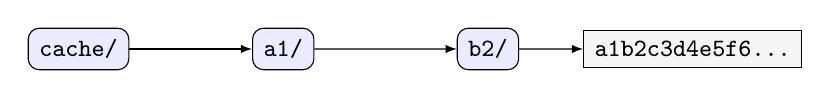
\begin{tikzpicture}[
        every node/.style={font=\ttfamily\small},
        grow=right, level distance=26mm,
        edge from parent/.style={draw, -latex},
        dir/.style={draw, rounded corners, fill=blue!8, inner sep=4pt},
        file/.style={draw, fill=gray!8, inner sep=4pt},
      ]
      \node[dir] {cache/}
        child { node[dir] {a1/}
          child { node[dir] {b2/}
            child { node[file] {a1b2c3d4e5f6\dots} }
          }
        };
    \end{tikzpicture}
    \caption{Sharded path for a cache key whose combined hash is \texttt{a1b2c3d4e5f6\dots}.}\label{dsn:shard-example}
  \end{figure}

  \reqdiaglink{global}{\textit{View complete diagram.}}

  \reqcover{verify}{TC}
  \reqcover{satisfy}{IMP}

  \refine{ADR-PERSISTENCE.MECHANISM-01}
  \satisfy{REQ-EFFICIENCY.DIRSCALE-01}
  \satisfy{FRE-COMPLIANCE.VARY-01}
  \satisfy{FRE-COMPLIANCE.VARYISOLATION-01}
  \trace{FDS-STORAGE.PUBLISH-01}
  \trace{ADR-EFFICIENCY.COMPACTION-01}
  \trace{FRE-COMPAT.STREAMING-01}

\end{requirement}

\begin{requirement}{FDS-LAYOUT.STARTUP-01}[draft][functionalRequirement]{Startup: shard directory cache}

  \localreqdiagram*{fdslayoutstartup01}{\reqid}{\reqdesc}

  \textbf{Two lifecycle moments, one cache.} The sharded tree of
  \reqref{SDS-LAYOUT.SHARDING-01} needs every shard directory to exist
  before an object's file can be created inside it. Checking that on every
  store, one file-system call at a time, is unnecessary: the tree is small
  and finite, so its existence can be established once, in memory, at
  construction, and consulted cheaply thereafter for the rest of the
  process's life, without depending on any state surviving a restart.

  \textbf{At construction.} Before the backend is handed to
  \texttt{HttpCache} as its \texttt{Storage} implementation, it shall
  ensure every first-level directory exists, creating any that are
  missing, and then, for each first-level directory, list its existing
  second-level subdirectories and record in an in-memory cache those named
  as \reqref{SDS-LAYOUT.SHARDING-01} names shards --- exactly two lowercase
  hexadecimal digits --- since anything else in the tree is not the
  backend's. This
  work is proportional only to the number of first- and second-level
  directories actually present --- at most 256 directory creations and 256
  directory listings --- never to the number of objects the cache holds,
  unlike \reqref{FDS-EVICTION.STARTUP-01}'s per-object scan. Because the
  cache is rebuilt this way at every start, it never depends on anything
  surviving a restart or a hot upgrade (\reqref{FRE-COMPAT.HOTUPGRADE-01}).

  \textbf{On each store.} A store already knows which shard its object
  belongs to (\reqref{SDS-LAYOUT.SHARDING-01}); the first-level directory
  is guaranteed to exist by construction, so only the second-level
  directory needs a decision. The backend shall consult the in-memory
  cache before creating an object's file: if the shard is already known,
  it proceeds directly; if not, it creates the second-level directory ---
  tolerating a concurrent store that reaches the same new shard first ---
  and adds it to the cache before proceeding. Because
  \reqref{SDS-LAYOUT.SHARDING-01} never removes a shard directory once
  created, the cache is purely additive: entries are only ever added, so
  none ever needs to be invalidated or re-checked against the file system.
  Something outside the backend may still remove a directory: IF creating a
  store's temporary fails because a shard directory the cache records as
  existing is missing, THEN the backend shall create that directory again
  and retry the creation once, and return a second failure as the store's
  error (\reqref{FRE-COMPAT.WRITEFAIL-01}).

  \textbf{Concurrency.} \texttt{Storage} is called from multiple threads at
  once (\reqref{FRE-COMPAT.CONCURRENT-01}), so the cache shall be safe for
  concurrent reads and inserts. Inserting an already-present shard shall be
  a harmless no-op --- two stores racing to create the same new shard both
  succeed, and both insertions land safely. The whole
  second-level namespace is small enough to track exactly, without
  approximation: a bitset over all 65,536 possible shards
  (\reqref{SDS-LAYOUT.SHARDING-01}) needs only 8~KiB.

  \begin{figure}[H]
    \centering
    \begin{adjustbox}{max width=\textwidth}
    \begin{sequencediagram}
      \newinst[0.0]{Integrator}{\guillemotleft actor\guillemotright\ Integrator}
      \newinst[0.5]{Storage}{Storage}
      \newinst[2.2]{DirectoryCache}{DirectoryCache}
      \newinst[0.5]{FileSystem}{File System}
      \begin{sdalt}{strict}{[at construction]}
        \begin{call}{Integrator}{new()}{Storage}{}
          \begin{call}{Storage}{mkdir() (each of 256 first-level dirs)}{FileSystem}{}
          \end{call}
          \begin{call}{Storage}{readdir() (each first-level dir)}{FileSystem}{existing shards}
          \end{call}
          \begin{call}{Storage}{insert(existing shards)}{DirectoryCache}{}
          \end{call}
        \end{call}
      \sdpart{[on each store, once traffic begins]}
        \begin{call}{Storage}{contains(shard)?}{DirectoryCache}{known / unknown}
        \end{call}
        \begin{call}{Storage}{mkdir(shard) if unknown (tolerate EEXIST)}{FileSystem}{}
        \end{call}
        \begin{call}{Storage}{insert(shard) if unknown}{DirectoryCache}{}
        \end{call}
      \end{sdalt}
    \end{sequencediagram}
    \end{adjustbox}
    \caption{Shard-directory cache: built once at construction by scanning
    the existing tree, then consulted (and grown) on each store. The
    \emph{strict} fragment marks its two regions as strictly sequential ---
    construction always completes before the backend is handed to
    \texttt{HttpCache}.}\label{fig:fds-layout-startup-seq}
  \end{figure}

  \reqdiaglink{global}{\textit{View complete diagram.}}

  \reqexpect{verify}{TC-LAYOUT.DIRCACHE-01}{Verify the cache is rebuilt
  accurately from disk at every construction, and that concurrent
  first-time stores into the same shard never fail or double-create.}
  \reqcover{satisfy}{IMP}

  \refine{SDS-LAYOUT.SHARDING-01}
\end{requirement}

\begin{requirement}{SDS-LAYOUT.OBJECTFILE-01}[draft][structuralRequirement]{Object-file record layout}

  \localreqdiagram*{dsn2}{\reqid}{\reqdesc}

  Each cache object is persisted as one self-describing \emph{record} --- the
  internal layout of the single file of \reqref{ADR-STORAGE.OBJECTFILE-01}. The
  record has four parts, in file order
  (Figure~\ref{dsn:singlefile-strip}): a fixed-size \emph{record header}, the
  object's serialised
  \texttt{CompactCacheKey}\footnote{\pgsrc{pingora-cache/src/key.rs}{153}{\texttt{struct CompactCacheKey}}.},
  a \emph{metadata region} of
  recorded capacity holding the object's two metadata segments plus free
  headroom for their growth, and the body bytes.

  \textbf{Metadata exactly as \texttt{pingora-cache} hands it over.} A
  \texttt{CacheMeta} serialises to two opaque byte segments --- the
  \emph{internal metadata} (the framework's created/updated instants,
  freshness deadline, and variance hash, MessagePack-encoded) and the
  \emph{header metadata} (status, protocol version, and header fields in the
  framework's own header encoding) --- and is rebuilt by
  \texttt{CacheMeta::deserialize(internal, header)}; the stock
  \texttt{MemCache} keeps precisely this pair per object. The record stores
  the same two segments byte for byte and never parses or edits them, so the
  round-trip fidelity duties on header fields and freshness inputs
  (\reqref{FRE-COMPLIANCE.HEADERS-01}, \reqref{FRE-COMPLIANCE.FRESHNESS-01})
  are met by construction: lookup returns what store received.

  \textbf{Record header: one aligned block.} The record header is a single
  44-byte block at offset~0, written and read as one unit: every field is a
  fixed-width little-endian integer at a naturally aligned offset (the
  \texttt{u64} at offset~8, every other field a \texttt{u32} at a multiple
  of four), so the block is saved by writing an
  in-memory \texttt{\#[repr(C)]} struct's bytes verbatim and read back by
  reading the block straight into that struct --- no field-by-field parsing,
  and byte swapping only on a big-endian host, as each field is read or
  written. No byte is spent on
  alignment filler: \texttt{version} and \texttt{key\_len} are each a
  \texttt{u32} rather than the \texttt{u16} their own range would need, so
  they close the gap that natural alignment would otherwise leave before
  \texttt{body\_len} and \texttt{internal\_len} respectively, instead of
  leaving it as unnamed padding. A future format revision that needs more
  header fields is free to define a different layout under a new
  \texttt{version}; nothing here is reserved against that in advance.
  Figure~\ref{dsn:singlefile-header} shows the byte placement; the fields are:
  \begin{itemize}
    \item \texttt{magic} (u32, offset 0) and \texttt{version} (u32, offset 4):
      identify the record format and its revision, so a scan can recognise
      records and a later revision can evolve the layout. \texttt{magic} is
      the four bytes \texttt{PDCR} (the little-endian value
      \texttt{0x52434450}); this layout is \texttt{version}~1. The version is
      the backend's own: it changes whenever records written before would no
      longer be read back exactly --- a change to this layout, or a
      \texttt{pingora-cache} release whose metadata encoding differs
      (\reqref{FRE-COMPAT.FORMATUPGRADE-01}) --- and a reader treats a record
      of any other version as a miss. Version~0 marks a record
      \emph{withdrawn} because its metadata outgrew the region (below), and
      is never a format version.
    \item \texttt{body\_len} (u64, offset 8): the body's exact byte length,
      patched at store completion.
    \item \texttt{meta\_capacity} (u32, offset 16): the byte size of the
      metadata region as allocated in \emph{this} record.
    \item \texttt{key\_len} (u32, offset 20): the length of the serialised
      \texttt{CompactCacheKey}, which is not constant across records: only
      \texttt{primary} (16 bytes) is
      fixed-size,\footnote{\pgsrc{pingora-cache/src/key.rs}{154}{\texttt{primary:
      HashBinary}} is a \texttt{[u8; 16]}.} while
      \texttt{variance}\footnote{\pgsrc{pingora-cache/src/key.rs}{156}{\texttt{variance:
      Option<Box<HashBinary>>}}: absent for a key with no \texttt{Vary}
      variant, 16 bytes when present.} is present or absent per key and
      \texttt{user\_tag}\footnote{\pgsrc{pingora-cache/src/key.rs}{157}{\texttt{user\_tag:
      Box<str>}}, ``the len should be small to keep memory usage bounded''
      per its own source comment --- guidance, not a fixed width.} is an
      arbitrary-length string; \texttt{key\_len} is what lets a reader
      locate the metadata region without assuming a size. The key segment's
      encoding is \reqref{SDS-LAYOUT.KEYSEGMENT-01}'s.
    \item \texttt{internal\_len} (u32, offset 24) and \texttt{header\_len}
      (u32, offset 28): the current lengths of the two metadata segments.
    \item \texttt{meta\_crc} (u32, offset 32): CRC-32C over the key and the
      two metadata segments.
    \item \texttt{body\_crc} (u32, offset 36): CRC-32C over the body's
      \texttt{body\_len} bytes, recorded at store completion
      (\reqref{ADR-PERSISTENCE.DURABILITY-01}); zero in a build without the
      \texttt{body-crc} feature. A reader never checks a stored zero.
    \item \texttt{header\_crc} (u32, offset 40): CRC-32C over header bytes
      0--39.
  \end{itemize}
  Every checksum in the record uses CRC-32C (the Castagnoli polynomial).

  \textbf{Segment placement.} The key segment starts immediately after the
  header, at offset 44, and the metadata region immediately after the key,
  with no padding: every segment is read into its own buffer, never
  interpreted in place, so none needs alignment. The region holds the
  internal and header segments back-to-back, followed by free headroom. Its capacity is fixed when the
  record is created --- the combined size of the segments actually presented
  (there is no fixed cap, so an arbitrarily large header set simply yields a
  larger region, \reqref{FRE-COMPLIANCE.HEADERS-01}) plus the configured
  growth headroom (\reqref{FDS-STORAGE.METAUPDATE-01}), a deployment setting
  defaulting to 512 bytes. The capacity is
  \emph{recorded} in \texttt{meta\_capacity}, so a reader computes the body
  offset (44 + \texttt{key\_len} + \texttt{meta\_capacity}) from the record
  alone and records written under
  different configurations coexist. The body follows, to the end of the file.

  \textbf{Why the key is stored.} The file is \emph{named} by the combined
  hash (\reqref{SDS-LAYOUT.SHARDING-01}), which cannot be inverted back to the
  key, while eviction admissions and purges are keyed by the
  \texttt{CompactCacheKey}.\footnote{\pgsrc{pingora-cache/src/eviction/mod.rs}{252}{\texttt{EvictionManager::admit}}
  takes a \pgsrc{pingora-cache/src/eviction/mod.rs}{53}{\texttt{CacheEntryKey}} and
  \pgsrc{pingora-cache/src/storage.rs}{194}{\texttt{Storage::purge}} a
  \pgsrc{pingora-cache/src/storage.rs}{51}{\texttt{PurgeTarget}}; both are thin
  wrappers that carry a \texttt{CompactCacheKey} and, for a backend that assigns
  them, an entry identifier this backend does not
  (\reqref{ADR-COMPAT.ENTRYID-01}). The key each needs is therefore the same
  \texttt{CompactCacheKey}.} The key segment is what lets the startup scan of
  \reqref{FDS-EVICTION.STARTUP-01} recover \texttt{admit(key, size,
  fresh\_until)} for every persisted entry --- the key from the key segment,
  the size as the record's file length (the record size
  \reqref{FRE-COMPAT.EVICTION-01} defines), the freshness deadline from the
  deserialised metadata --- reading only the header, key, and metadata region,
  never the body (\reqref{FRE-COMPAT.EVICTION-01}). It also lets any
  reader confirm a record matches the key it looked up, catching a
  wrong-shard read caused by a software defect or on-disk corruption, and
  lets the restart scan reclaim a record found anywhere but at its own key's
  path (\reqref{FDS-STORAGE.RECLAIM-01}).

  \textbf{A weaker collision guard than it looks.} That confirmation is not
  a defence against a genuine hash collision for every key: a key with
  neither a variance nor a user tag has \texttt{CompactCacheKey}'s
  \texttt{primary} field exactly equal to the combined hash that named its
  file (\reqref{SDS-LAYOUT.SHARDING-01}), so two different keys
  colliding there would carry identical stored keys too and go undetected.
  Only a varianced key gets a real check, because its stored
  \texttt{primary} and \texttt{variance} survive as the separate values
  they were before \texttt{combined\_bin} folded them together
  (\reqref{SDS-LAYOUT.SHARDING-01}) --- a collision in that folding step is
  independent of a collision in either value alone. No comparable cache
  pays for a stronger guarantee across the board: the stock
  \texttt{MemCache} trusts the combined hash as its map key with no
  comparison at
  all,\footnote{\pgsrc{pingora-cache/src/memory.rs}{313}{\texttt{MemCache::lookup}}
  looks an object up by \texttt{key.combined()} alone --- whatever is
  stored under that hash is returned unconditionally.} and Traffic
  Server's on-disk record stores only hashes of the key, never the
  original URL, so its own read-time check is exactly as hash-bound as
  this one.\footnote{\texttt{first\_key} and \texttt{key} are both a
  \texttt{CryptoHash}, never the request URL itself.
  \href{https://github.com/apache/trafficserver/blob/10.1.4/src/iocore/cache/P_CacheDoc.h\#L45-L49}{Apache
  Traffic Server source (release 10.1.4):
  \texttt{src/iocore/cache/P\_CacheDoc.h}, lines 45--49}.} Keying storage
  on the full, unhashed request string instead --- as Caddy's Souin-based
  cache module does\footnote{\href{https://github.com/darkweak/souin/blob/v1.7.8/context/key.go\#L147}{Souin
  source (release v1.7.8): \texttt{context/key.go}, line 147} builds the
  storage key by concatenating the method, scheme, host, path, query, and
  varied header values verbatim, never folding them into a fixed-size
  hash.} --- would remove the question entirely, at the cost of storing,
  and comparing on every lookup, a full request string that is typically
  far longer than the 16-byte hashes this record carries.

  \textbf{Write, publication, and integrity.} The header, key, and metadata
  region are written when the store's miss handler
  opens\footnote{\pgsrc{pingora-cache/src/storage.rs}{176}{\texttt{Storage::get\_miss\_handler}}
  hands the backend the \texttt{CacheMeta} directly, before any body bytes
  arrive.} --- the
  \texttt{CacheMeta} is available then; body
  chunks are appended as they stream in, each folded into a running CRC-32C
  kept in memory unless the build leaves out the \texttt{body-crc} feature.
  While the per-writer temporary grows
  (\reqref{SDS-LAYOUT.SHARDING-01}), the valid length lives in the in-memory
  in-flight registry that backs streaming partial hits
  (\reqref{FDS-STORAGE.PARTIAL-01}); the on-disk header is \emph{not}
  the source of truth for readers of an in-flight write. At completion the
  backend patches \texttt{body\_len} and \texttt{body\_crc}, recomputes
  \texttt{header\_crc}, synchronises the file's data to stable storage, and
  renames the temporary to the canonical name
  (\reqref{FDS-STORAGE.PUBLISH-01}, \reqref{ADR-PERSISTENCE.DURABILITY-01}).

  A reader accepts a published record only if, in this order: the magic and
  \texttt{version} match this layout's; \texttt{header\_crc} verifies; the
  metadata segments fit within \texttt{meta\_capacity}; the computed body
  offset lies within the file; \texttt{meta\_crc} verifies (with the
  re-reads described under in-place updates below); the stored key equals the
  looked-up key; and the file's length is \emph{exactly} the computed body
  offset plus \texttt{body\_len}. The two bounds come before the reader
  sizes any read by a length the header carries, so no header, however
  forged, makes it allocate or read beyond the file. Any failure --- a truncated
  file, a torn or foreign record --- makes the lookup report a miss, so a
  damaged record is never served (\reqref{FRE-COMPLIANCE.INCOMPLETE-01}). The
  reader does not remove the file: a later store of the same key replaces it,
  and the restart-time scan reclaims it (\reqref{FDS-STORAGE.RECLAIM-01}),
  so a lookup never unlinks a path whose content may have changed since it
  opened it. A reader does not check the body against \texttt{body\_crc}:
  integrity at rest is the storage layer's
  (\reqref{ADR-PERSISTENCE.DURABILITY-01}). A build with the
  \texttt{body-crc-verify} feature can switch a check on in its
  configuration: a reader that streams the whole body from its start then
  computes CRC-32C over the bytes it delivers and, at the end, compares it
  with \texttt{body\_crc}; on a mismatch it logs an error naming the file and
  still ends the stream normally, since every byte has already been
  delivered. A published record supports seeking: its hit handler reports
  \texttt{can\_seek}, and a seeked read delivers exactly the requested slice
  (\reqref{FRE-COMPLIANCE.BODY-01}) and is never checked, since the checksum
  covers only a whole body. Figure~\ref{fig:sds-objectfile-lookup-seq}
  shows the read path this validation belongs to.

  \begin{figure}[H]
    \centering
    \begin{adjustbox}{max width=\textwidth}
    \begin{sequencediagram}
      \newinst[0.0]{HttpCache}{HttpCache}
      \newinst[3.7]{Storage}{Storage}
      \begin{call}{HttpCache}{lookup(key)}{Storage}{(CacheMeta, HitHandler) / None}
        \postlevel
        \postlevel
        \postlevel
        \begin{callself}{Storage}{{\small \shortstack{no in-flight write for the key (\reqref{FDS-STORAGE.PARTIAL-01});\\compute combined hash (\reqref{SDS-LAYOUT.SHARDING-01});\\open file at shard path; read 44-byte header}}}{}
        \end{callself}
        \begin{sdalt}{alt}{[magic, version, CRCs, key, and length all valid]}
          \postlevel
          \begin{callself}{Storage}{{\small \shortstack{deserialise CacheMeta from internal + header segments}}}{}
          \end{callself}
        \sdpart{[any single check fails --- damaged, incomplete, or foreign]}
          \postlevel
          \begin{callself}{Storage}{{\small treat as a miss; leave the file}}{}
          \end{callself}
        \end{sdalt}
      \end{call}
      \begin{sdalt}{loop}{[on a hit: read\_body() until exhausted]}
        \begin{call}{HttpCache}{read\_body()}{Storage}{chunk / None at EOF / error}
          \postlevel
          \postlevel
          \begin{callself}{Storage}{{\small \shortstack{read the next slice from the validated body offset}}}{}
          \end{callself}
        \end{call}
      \end{sdalt}
    \end{sequencediagram}
    \end{adjustbox}
    \caption{Lookup/read sequence for a published record (an in-flight write
    of the key is served first, as \reqref{FDS-STORAGE.PARTIAL-01}
    specifies): the reader recomputes the file's own path from the key,
    opens it, and validates the record before trusting it. Any single
    validation failure --- a bad magic or version, a CRC mismatch, a
    different stored key, or a length that is not exactly
    the computed body offset plus \texttt{body\_len} --- is indistinguishable
    from any other: the lookup reports a miss and leaves the file for a later
    store or the restart-time scan
    (\reqref{FRE-COMPLIANCE.INCOMPLETE-01}, verified by
    \reqref{TC-LAYOUT.OBJECTFILE-01}). On a hit, the already-validated file
    stays open and every \texttt{read\_body} call simply advances through
    it; unlike Figure~\ref{fig:fds-publish-seq}'s concurrent
    \texttt{Follower}, this reader never races a body append, since the
    file it opened was already published at open time (an in-place
    metadata update may still race the metadata read, handled by the
    re-reads described below).}\label{fig:sds-objectfile-lookup-seq}
  \end{figure}

  \textbf{Metadata updates in place.} A metadata update
  (\reqref{FRE-COMPLIANCE.REVALIDATION-01}) whose new segments fit
  \texttt{meta\_capacity} --- the reserved headroom decided in
  \reqref{FDS-STORAGE.METAUPDATE-01} --- is applied in place: the segments
  are rewritten in the region, then \texttt{internal\_len},
  \texttt{header\_len}, and the CRCs are updated --- the body is never
  touched --- and nothing is synchronised to stable storage
  (\reqref{ADR-PERSISTENCE.DURABILITY-01}). A reader that catches the update
  mid-write sees a CRC mismatch and re-reads the header and metadata region,
  up to three more times, yielding to other tasks between attempts. If all
  four reads mismatch --- the updater may have been stopped between its two
  writes --- the lookup reads once more holding the key's publication lock
  (\reqref{FDS-STORAGE.METAUPDATE-01}), which every metadata update holds
  from its first write to its last, so that this read finds the record
  whole. Only if that read mismatches too does the lookup report a miss and
  leave the file, as for any damaged record; the restart scan reads such a
  record once more in the same way before it reclaims it
  (\reqref{FDS-STORAGE.RECLAIM-01}). A reader therefore observes
  the pre- or post-update set, never a mixture, and an update in progress
  never turns a hit into a miss. This assumes nothing about the write itself being atomic ---
  no POSIX filesystem or disk interface guarantees that a multi-byte write
  lands as one indivisible unit, even for a single nominal sector or
  page,\footnote{\href{https://www.sqlite.org/atomiccommit.html}{SQLite
  documentation: ``Atomic Commit In SQLite''}: ``SQLite has traditionally
  assumed that a sector write is not atomic.''} the metadata region can
  exceed any one write unit once the header set is large enough (there is
  no fixed cap on it), and the update spans two separate byte ranges ---
  the metadata region and the header block's own length fields --- that no
  single write covers together regardless. Treating this as a live, not
  theoretical, risk matches established practice: PostgreSQL's
  \texttt{full\_page\_writes} exists because ``a page write that is in
  process during an operating system crash might be only partially
  completed, leading to an on-disk page that contains a mix of old and new
  data,''\footnote{\href{https://www.postgresql.org/docs/18/runtime-config-wal.html\#GUC-FULL-PAGE-WRITES}{PostgreSQL
  18 documentation: \texttt{full\_page\_writes}}.} and MySQL's InnoDB
  doublewrite buffer exists for the identical reason, recovering a good
  copy when a crash lands ``in the middle of a page
  write.''\footnote{\href{https://dev.mysql.com/doc/refman/8.0/en/innodb-doublewrite-buffer.html}{MySQL
  8.0 Reference Manual: ``Doublewrite Buffer''}.} A cheaper-looking
  alternative --- marking the record \emph{writing} before the update and
  \emph{done} after, so only the rare writer pays a check instead of every
  reader --- does not remove the requirement: without an explicit ordering
  barrier between the status write and the payload write, the file system
  is free to persist them out of order --- \texttt{fsync} only flushes
  ``modified in-core data\ldots{} to the disk device,'' so anything not yet
  flushed simply sits reorderable in the page cache until it
  is,\footnote{\href{https://man7.org/linux/man-pages/man2/fsync.2.html}{Linux
  manual page: \texttt{fsync(2)}}.} and a crash could therefore leave a
  durable \emph{done} status covering a payload that never actually
  landed. Enforcing that ordering costs at least one synchronous flush per
  write --- PostgreSQL's own documentation calls exactly this delay ``a
  major component of the total transaction time'' for short transactions,
  the reason its asynchronous-commit mode exists at
  all,\footnote{\href{https://www.postgresql.org/docs/current/wal-async-commit.html}{PostgreSQL
  documentation: ``Asynchronous Commit''}.} typically millisecond-scale on
  hardware without power-loss
  protection\footnote{\href{https://smalldatum.blogspot.com/2026/01/ssds-power-loss-protection-and-fsync.html}{Mark
  Callaghan, ``Small Datum'': ``SSDs, power loss protection and fsync
  latency''}: consumer SSDs measured at roughly 1--5~ms per
  \texttt{fsync}, versus under 0.1~ms for enterprise drives with
  power-loss protection.} --- far more than the microsecond-scale check it
  would replace. Nor is the read-side check adding a separate cost to
  shift in the first place: \texttt{CacheMeta::deserialize} already needs
  the whole internal and header byte range in memory to decode it, so the
  CRC recompute is one more pass over bytes already resident from the read
  that just happened, not a second read or a meaningfully separate
  computation.

  \textbf{Metadata that outgrows the region.} When the new metadata no
  longer fits \texttt{meta\_capacity}, the record is \emph{withdrawn}
  instead (\reqref{FDS-STORAGE.METAUPDATE-01}): only its header is
  rewritten, with \texttt{version}~0 and \texttt{header\_crc} resealed.
  Every reader then treats the key as holding no object, so the next request
  fetches it again, and its store, sized for the new metadata, replaces the
  file; until then the file keeps its length, and the space the eviction
  manager counts for it. The body is neither read nor moved, and a reader
  that catches the header write midway sees a checksum or version mismatch
  and ends with the record whole or a miss, never a mixture. The reserved
  headroom is what makes the common freshening after a \texttt{304}
  (\texttt{Date}- and \texttt{Age}-scale changes) an in-place write rather
  than a withdrawal and a fetch from the origin. Moving outgrown metadata
  after the body instead, which would spare that fetch, is deferred to a
  later version (\reqref{ADR-STORAGE.METAMOVE-01}).

  \textbf{Self-delimiting for future reuse.} The record is self-delimiting ---
  header, key length, capacity, and body length define its exact extent.
  Object compaction into shared aggregate files is not implemented for this
  version (\reqref{ADR-EFFICIENCY.COMPACTION-01}); this property is what
  would let a future version move a completed record verbatim, back-to-back
  with others, into an aggregate without redesigning it, and let such an
  aggregate be re-scanned sequentially --- for recovery or startup
  enumeration --- without a separate index.

  \begin{figure}[H]
    \centering
    \begin{subfigure}{\textwidth}
      \centering
      \begin{adjustbox}{max width=\textwidth}
      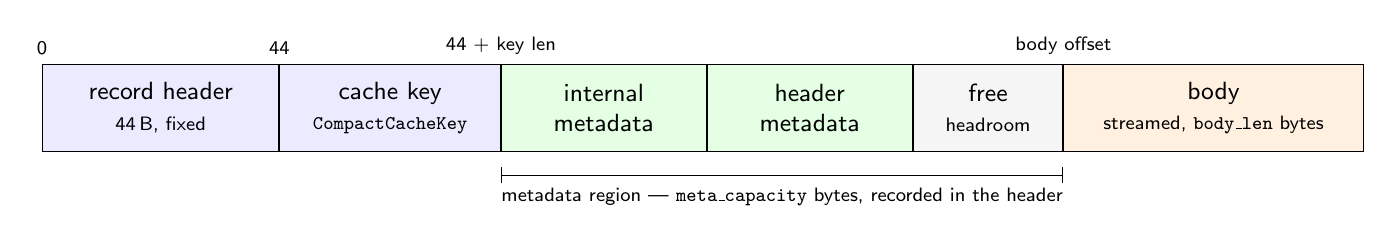
\begin{tikzpicture}[
          font=\small,
          seg/.style={draw, minimum height=11mm, align=center, anchor=west, inner sep=3pt},
        ]
        \node[seg, fill=blue!8,    minimum width=30mm] (hdr) at (0,0)      {record header\\{\scriptsize 44\,B, fixed}};
        \node[seg, fill=blue!8,    minimum width=28mm] (key) at (hdr.east) {cache key\\{\scriptsize\ttfamily CompactCacheKey}};
        \node[seg, fill=green!10,  minimum width=26mm] (im)  at (key.east) {internal\\metadata};
        \node[seg, fill=green!10,  minimum width=26mm] (hm)  at (im.east)  {header\\metadata};
        \node[seg, fill=gray!8,    minimum width=19mm] (fr)  at (hm.east)  {free\\{\scriptsize headroom}};
        \node[seg, fill=orange!12, minimum width=38mm] (bd)  at (fr.east)  {body\\{\scriptsize streamed, \texttt{body\_len} bytes}};
        \node[font=\scriptsize, anchor=south] at (hdr.north west) {0};
        \node[font=\scriptsize, anchor=south] at (key.north west) {44};
        \node[font=\scriptsize, anchor=south] at (im.north west)  {44 + key len};
        \node[font=\scriptsize, anchor=south] at (bd.north west)  {body offset};
        \draw[{Bar}-{Bar}] ([yshift=-3mm]im.south west) -- node[below=1pt, font=\scriptsize]{metadata region --- \texttt{meta\_capacity} bytes, recorded in the header} ([yshift=-3mm]fr.south east);
      \end{tikzpicture}
      \end{adjustbox}
      \caption{The record's segments in file order.}\label{dsn:singlefile-strip}
    \end{subfigure}

    \medskip

    \begin{subfigure}{\textwidth}
      \centering
      \begin{adjustbox}{max width=0.85\textwidth}
      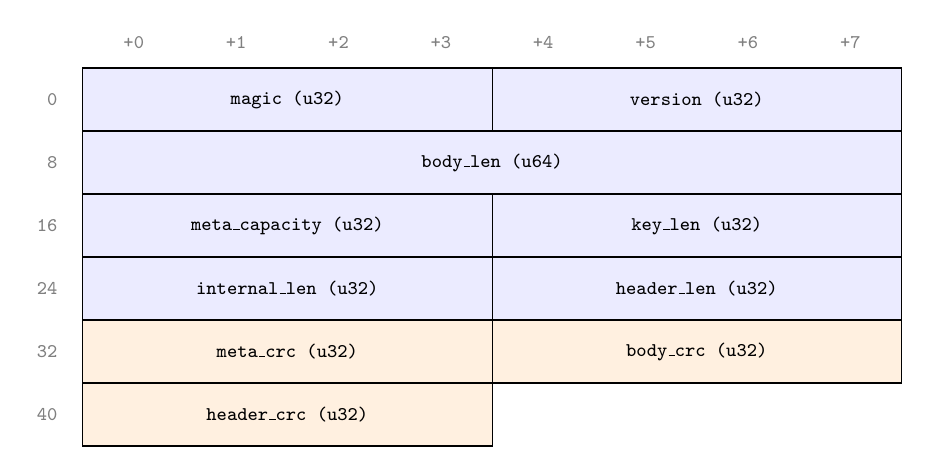
\begin{tikzpicture}[x=13mm, y=8mm, font=\ttfamily\scriptsize]
        \foreach \c in {0,...,7} {\node[gray] at (\c+0.5, 0.4) {+\c};}
        \foreach \r/\o in {0/0, 1/8, 2/16, 3/24, 4/32, 5/40}
          {\node[gray, anchor=east] at (-0.15, -\r-0.5) {\o};}
        \draw[fill=blue!8]    (0,-1) rectangle (4,0);   \node at (2,-0.5) {magic (u32)};
        \draw[fill=blue!8]    (4,-1) rectangle (8,0);   \node at (6,-0.5) {version (u32)};
        \draw[fill=blue!8]    (0,-2) rectangle (8,-1);  \node at (4,-1.5) {body\_len (u64)};
        \draw[fill=blue!8]    (0,-3) rectangle (4,-2);  \node at (2,-2.5) {meta\_capacity (u32)};
        \draw[fill=blue!8]    (4,-3) rectangle (8,-2);  \node at (6,-2.5) {key\_len (u32)};
        \draw[fill=blue!8]    (0,-4) rectangle (4,-3);  \node at (2,-3.5) {internal\_len (u32)};
        \draw[fill=blue!8]    (4,-4) rectangle (8,-3);  \node at (6,-3.5) {header\_len (u32)};
        \draw[fill=orange!12] (0,-5) rectangle (4,-4);  \node at (2,-4.5) {meta\_crc (u32)};
        \draw[fill=orange!12] (4,-5) rectangle (8,-4);  \node at (6,-4.5) {body\_crc (u32)};
        \draw[fill=orange!12] (0,-6) rectangle (4,-5);  \node at (2,-5.5) {header\_crc (u32)};
      \end{tikzpicture}
      \end{adjustbox}
      \caption{The 44-byte record header: fixed-width little-endian fields at
        naturally aligned offsets (row offsets left, byte positions above), so
        the block round-trips between disk and a \texttt{\#[repr(C)]} struct
        without repacking.}\label{dsn:singlefile-header}
    \end{subfigure}
    \caption{Object-file record layout: the on-disk structure of one cache
      object. Its self-delimiting fields are also what would let a future
      version reuse it, unchanged, inside an aggregate file
      (\reqref{ADR-EFFICIENCY.COMPACTION-01}).}\label{dsn:singlefile-layout}
  \end{figure}

  \textit{Basis: \pgsrc{pingora-cache/src/memory.rs}{38}{\texttt{MemCache}'s
  per-object metadata pair \texttt{BinaryMeta = (Vec<u8>, Vec<u8>)}} and its
  \pgsrc{pingora-cache/src/memory.rs}{45}{\texttt{TempObject}} (in-memory
  tracking of an in-flight write's valid length);
  \pgsrc{pingora-cache/src/meta.rs}{890}{\texttt{CacheMeta::serialize}} /
  \pgsrc{pingora-cache/src/meta.rs}{898}{\texttt{deserialize(internal,
  header)}}; internal-metadata fields per
  \pgsrc{pingora-cache/src/meta.rs}{83}{\texttt{InternalMetaV2}}.}

  \reqdiaglink{global}{\textit{View complete diagram.}}

  \reqexpect{refine}{SDS-LAYOUT.KEYSEGMENT-01}{Specify the key segment's
  byte encoding --- its fields' order and sizes, how the presence of a
  variance hash is marked, and how the tag is delimited --- so that each key
  has exactly one encoding.}
  \reqexpect{verify}{TC-LAYOUT.OBJECTFILE-01}{Verify that a reader accepts a
  record only when its magic, version, header and metadata CRCs, and stored
  key all validate, its metadata segments fit its capacity, its body offset
  lies within the file, and the file's length is exactly the
  computed body offset plus body_len; that any single violation is a miss
  and leaves the file in place; that a body whose checksum mismatches is read
  to a normal end, and is logged when the read-time check is on; and that a
  metadata read racing an in-place update returns one complete version.}
  \reqcover{satisfy}{IMP}

  \refine{ADR-STORAGE.OBJECTFILE-01}
  \refine{ADR-PERSISTENCE.DURABILITY-01}
  \satisfy{FRE-COMPAT.FORMATUPGRADE-01}
  \satisfy{FRE-COMPLIANCE.INCOMPLETE-01}
  \satisfy{FRE-COMPLIANCE.HEADERS-01}
  \satisfy{FRE-COMPLIANCE.FRESHNESS-01}
  \satisfy{FRE-COMPLIANCE.VALIDATORS-01}
  \satisfy{FRE-COMPLIANCE.BODY-01}
  \satisfy{FRE-COMPLIANCE.TRAILERS-01}
  \trace{FDS-STORAGE.PUBLISH-01}
  \trace{FDS-STORAGE.METAUPDATE-01}
  \trace{ADR-EFFICIENCY.COMPACTION-01}
  \trace{FRE-COMPLIANCE.REVALIDATION-01}
  \trace{FRE-COMPAT.EVICTION-01}
  \trace{FRE-COMPAT.STREAMING-01}
  \trace{FDS-EVICTION.STARTUP-01}
  \trace{SDS-LAYOUT.SHARDING-01}

\end{requirement}

\begin{requirement}{SDS-LAYOUT.KEYSEGMENT-01}[draft][structuralRequirement]{Key segment encoding}

  \localreqdiagram*{dsn3}{\reqid}{\reqdesc}

  The key segment of a record (\reqref{SDS-LAYOUT.OBJECTFILE-01}) holds the
  object's
  \texttt{CompactCacheKey}\footnote{\pgsrc{pingora-cache/src/key.rs}{153}{\texttt{CompactCacheKey}}.}
  as these fields, in this order, with no padding between them:
  \begin{itemize}
    \item \texttt{primary} (16 bytes): the key's primary hash.
    \item The \emph{variance flag} (1 byte): 1 when a variance hash follows,
      0 when none does.
    \item \texttt{variance} (16 bytes): the key's variance hash, present
      exactly when the variance flag is 1.
    \item \texttt{user\_tag}: the tag's UTF-8 bytes, filling the rest of the
      segment.
  \end{itemize}
  Both hashes are
  \texttt{HashBinary}\footnote{\pgsrc{pingora-cache/src/key.rs}{26}{\texttt{HashBinary}}
  is a \texttt{[u8; 16]}.} values. The tag carries no length of its own: the
  header's \texttt{key\_len} bounds the segment, so whatever follows the
  fixed fields is the tag. Each key therefore has exactly one encoding, which
  is what lets a reader compare a stored key with the key it looked up byte
  for byte.

  Only the restart-time scan decodes a stored key, to rebuild the
  \texttt{CompactCacheKey} it admits to the eviction manager
  (\reqref{FDS-EVICTION.STARTUP-01}). IF a key segment is shorter than the
  fields its variance flag announces, carries a variance flag other than 0 or
  1, or holds a tag that is not valid UTF-8, THEN the restart-time scan shall
  reclaim the record as damaged (\reqref{FDS-STORAGE.RECLAIM-01}).

  The field sizes are part of the record format: a \texttt{pingora-cache}
  release that changed the size of \texttt{HashBinary} would change what is
  stored, and so would require a new format version
  (\reqref{FRE-COMPAT.FORMATUPGRADE-01}).

  \reqdiaglink{global}{\textit{View complete diagram.}}

  \reqexpect{verify}{TC-LAYOUT.KEYSEGMENT-01}{Verify that keys with and
  without a variance hash, and with an empty and a non-empty tag, encode to
  the specified layout and decode back to themselves; that a segment too
  short for its fields, a variance flag other than 0 or 1, and a tag that is
  not UTF-8 are each rejected; and that the restart-time scan reclaims a
  record whose key does not decode.}
  \reqcover{satisfy}{IMP}

  \refine{SDS-LAYOUT.OBJECTFILE-01}
  \trace{FDS-EVICTION.STARTUP-01}
  \trace{FDS-STORAGE.RECLAIM-01}
  \trace{FRE-COMPAT.FORMATUPGRADE-01}
\end{requirement}


\begin{requirement}{FDS-EVICTION.STARTUP-01}[draft][functionalRequirement]{Startup: reconstruction procedure}

  \localreqdiagram*{fdsstartup01}{\reqid}{\reqdesc}

  \textbf{A dedicated API, not raw primitives.} The \texttt{Storage} trait
  has no startup lifecycle hook, so this reconstruction is orchestrated by
  \emph{Eviction Recovery}: a distinct API surface in the same crate as the
  \texttt{Storage} implementation, additional to it rather than folded into
  it, and --- unlike \texttt{CacheLock} or the \texttt{EvictionManager}
  itself --- never invoked \emph{per request}: it is called once per process
  start, possibly after serving has already begun. Exposing only primitives
  instead (enumerate persisted entries, an \texttt{admit} passthrough) would
  force every integrator to reimplement the same scan-and-reconcile
  sequencing below, and doing so from outside the crate would mean exposing
  the private on-disk object-record format this specification keeps
  internal everywhere else (\reqref{SDS-LAYOUT.OBJECTFILE-01}); folding it
  into a custom \texttt{EvictionManager} was already ruled out by
  \reqref{ADR-COMPAT.EVICTION-01}, which adopted the stock manager
  specifically to avoid building one. The cost is a second public API
  surface beyond \texttt{Storage}, with its own contract to document and
  version --- but a single one, safe to call unconditionally whether a
  first launch, a post-crash restart, or the new side of a hot upgrade
  (\reqref{FRE-COMPAT.HOTUPGRADE-01}): with no shutdown hook and no
  snapshot, there is nothing to call at the wrong time or to poison during
  a drain.

  \textbf{The procedure.} At process start, Eviction Recovery's
  \texttt{recover()} shall reconstruct the eviction manager from the published
  records, per \reqref{ADR-COMPAT.EVICTION-01}. On the incoming side of a hot
  upgrade the integrator calls it only once its server holds the listening
  sockets and the upgrade's close timeout has elapsed
  (\reqref{FDS-COMPAT.READONLY-01}). \texttt{recover()} enumerates the tree
  (\reqref{ADR-PERSISTENCE.MECHANISM-01}), classifying each entry as
  \reqref{FDS-STORAGE.RECLAIM-01} specifies, and admits every record it keeps
  with \texttt{admit(entry key, size, fresh\_until)}, where the entry key is the
  record's own \texttt{CompactCacheKey} carried in a \texttt{CacheEntryKey} with
  no entry identifier (\reqref{ADR-COMPAT.ENTRYID-01}) --- the same shape
  \texttt{HttpCache} builds for a live admission, so the two paths address one
  entry rather than two --- and \texttt{size} is the
  record size --- the file's length --- the same size a completed store
  reports (\reqref{FDS-STORAGE.PUBLISH-01}). Each \texttt{admit} may return
  eviction victims --- the manager deducts their sizes immediately and
  expects the caller to remove them from storage --- so the procedure shall
  purge every returned victim from \texttt{Storage} as an eviction, naming it by
  the exact entry the manager returned (\texttt{PurgeTarget::Exact}), exactly
  as \texttt{HttpCache} does after a live admission; a store found over its
  budget at startup is thereby brought back under it. Once the backend is
  read-only (\reqref{FDS-COMPAT.READONLY-01}), the procedure shall stop: it
  reads no further entry, and skips its remaining admissions and ghost-entry
  checks, since the eviction manager they would update is discarded when the
  process exits. It shall stop the same way, run by the hot-upgrade
  helper's recovery service, once the server starts shutting down
  (\reqref{FDS-COMPAT.READONLY-01}). \texttt{recover()}
  returns once enumeration and the reconciliation below have completed; that
  return is the backend reporting its restart procedure complete
  (\reqref{FRE-COMPAT.EVICTION-01}).

  \textbf{Running alongside live traffic.} Whether the integrator starts
  serving before \texttt{recover()} returns is its own choice
  (\reqref{ADR-COMPAT.EVICTION-01}). The manager keys entries by
  \texttt{CacheEntryKey}, which for this backend carries the
  \texttt{CompactCacheKey} and nothing more, so the scan and live traffic
  admitting the same object update one entry rather than duplicating it. The procedure shall
  close the races the decision identifies, each by acting while holding the
  key's publication lock (\reqref{FDS-STORAGE.METAUPDATE-01}), which a live
  store's rename also takes before that store is admitted:
  \begin{itemize}
    \item \emph{Stale size.} Immediately before admitting a record, the
      procedure re-checks its path under the lock. If the path is gone or
      now refers to a different file than the one read, it skips the record
      --- live traffic removed it, or published and will admit its
      replacement; otherwise it admits the record with the file's current
      length while still holding the lock.
    \item \emph{Ghost entries.} After enumeration, for every key it admitted,
      the procedure checks under the lock whether the canonical path still
      exists, and calls the manager's \texttt{remove} --- which takes the
      borrowed \pgsrc{pingora-cache/src/eviction/mod.rs}{169}{\texttt{CacheEntryKeyRef}}
      form of the same identity --- for any that does not.
      A key live traffic republishes after that check is admitted by the live
      path afterwards.
  \end{itemize}
  An object live traffic has just read may still come back from an
  \texttt{admit} as a victim; it is purged like any other, and accounting
  stays exact.

  \begin{figure}[H]
    \centering
    \begin{adjustbox}{max width=\textwidth}
    \begin{sequencediagram}
      \newinst[0.0]{Startup}{\guillemotleft actor\guillemotright\ Startup}
      \newinst[0.5]{EvictionRecovery}{Eviction Recovery}
      \newinst[5.4]{EvictionManager}{EvictionManager}
      \newinst[0.5]{Storage}{Storage}
      \newinst[0.5]{HttpCache}{HttpCache}
      \begin{sdalt}{par}{[timing is the integrator's choice]}
        \begin{call}{Startup}{recover()}{EvictionRecovery}{}
          \begin{call}{EvictionRecovery}{enumerate()}{Storage}{entries}
          \end{call}
          \begin{call}{EvictionRecovery}{admit(entry key, size, fresh\_until)}{EvictionManager}{victims}
          \end{call}
          \begin{call}{EvictionRecovery}{purge(Exact(victim), Eviction) (for each victim)}{Storage}{}
          \end{call}
          \begin{call}{EvictionRecovery}{remove(entry key) for each admitted key now absent}{EvictionManager}{}
          \end{call}
        \end{call}
      \sdpart{[begin serving, whenever chosen]}
        \begin{call}{Startup}{begin serving}{HttpCache}{}
          \begin{call}{HttpCache}{admit / access (live)}{EvictionManager}{}
          \end{call}
        \end{call}
      \end{sdalt}
    \end{sequencediagram}
    \end{adjustbox}
    \caption{Startup reconstruction, carried out by Eviction Recovery (\texttt{Storage} and the \texttt{EvictionManager} never call each other). \texttt{Startup} --- the integrator's own code --- independently calls \texttt{recover()} and, on its own schedule, tells \texttt{HttpCache} to begin serving; if serving starts before reconstruction finishes, live \texttt{HttpCache} traffic touches the \texttt{EvictionManager} in parallel with the scan.}\label{fig:fds-startup-seq}
  \end{figure}

  \reqdiaglink{global}{\textit{View complete diagram.}}

  \reqexpect{verify}{TC-EVICTION.RECONSTRUCT-01}{Verify that when recover()
  returns the manager holds exactly the published set with record sizes,
  including when stores, replacements, and purges run during the scan, and
  that no snapshot or delta log is read or written at any point.}
  \reqcover{satisfy}{IMP}

  \refine{ADR-COMPAT.EVICTION-01}
  \trace{ADR-PERSISTENCE.MECHANISM-01}
  \trace{FDS-COMPAT.READONLY-01}
  \trace{FDS-STORAGE.RECLAIM-01}
  \satisfy{FRE-COMPAT.EVICTION-01}
  \satisfy{FRE-COMPAT.HOTUPGRADE-01}
\end{requirement}

\begin{requirement}{FDS-COMPAT.READONLY-01}[draft][functionalRequirement]{Read-only on the upgrade signal}

  \localreqdiagram*{fdsreadonly01}{\reqid}{\reqdesc}

  \textbf{The read-only operation.} The backend shall expose a
  \texttt{set\_read\_only} operation, callable from any thread and
  idempotent, which the integrator calls when its server's execution-phase
  broadcast announces
  \texttt{GracefulUpgradeTransferringFds}.\footnote{\pgsrc{pingora-core/src/server/mod.rs}{235}{\texttt{Server::watch\_execution\_phase}}
  subscribes to the broadcast, which sends that phase when the upgrade signal
  arrives (\pgsrc{pingora-core/src/server/mod.rs}{279}{L279}).} A graceful
  terminate, which announces \texttt{GracefulTerminate} instead, does not
  call it: no incoming process will take over the cache, so stores that
  complete while sessions drain should still be published.

  \textbf{The read-only gate.} The backend shall keep a process-wide
  \emph{read-only} flag behind a read--write gate. Every durable change ---
  a store's final rename (\reqref{FDS-STORAGE.PUBLISH-01}), a purge's unlink
  (\reqref{FDS-STORAGE.PURGE-01}), either path of a metadata update
  (\reqref{FDS-STORAGE.METAUPDATE-01}) or of an expiry
  (\reqref{FDS-STORAGE.EXPIRE-01}), and a reclaim unlink
  (\reqref{FDS-STORAGE.RECLAIM-01}) --- holds the gate shared from the moment
  it checks the flag until the change is done. So does each of the restart
  scan's admission checks (\reqref{FDS-EVICTION.STARTUP-01}), which changes
  no file but takes a key's publication lock
  (\reqref{FDS-STORAGE.METAUPDATE-01}): every taker of that lock enters the
  gate first. \texttt{set\_read\_only} takes the gate exclusively to set the
  flag, so when it returns, nothing that entered the gate before it is still
  running, and nothing can enter afterwards.

  \textbf{Once read-only.} The process keeps draining its sessions; only its
  backend's changes to the shared cache stop. From then on the backend
  shall:
  \begin{itemize}
    \item keep opening stores and accepting their body writes, since failing
      to open a store would fail the client request that triggered
      it,\footnote{The proxy propagates the error from
      \pgsrc{pingora-proxy/src/proxy_cache.rs}{689}{\texttt{set\_miss\_handler}}
      with \texttt{?}.} and partial-hit readers inside this process
      (\reqref{FDS-STORAGE.PARTIAL-01}) keep streaming;
    \item in \texttt{finish}, remove the temporary instead of renaming it,
      while reporting the store created with its record size, so the request
      completes normally --- the entry this adds to the process's own
      eviction manager is discarded when the process exits;
    \item fail \texttt{purge} (of either purge type and either target kind),
      \texttt{expire}, and \texttt{update\_meta} with an error, changing nothing
      on disk;
    \item stop the restart scan, skipping any reclaim unlink and any
      admission check still pending --- the eviction manager the checks would
      update is discarded when the process exits;
    \item serve \texttt{lookup} and body reads unchanged.
  \end{itemize}

  \textbf{Ordering with the incoming process.} In the incoming process,
  Eviction Recovery's \texttt{recover()} (\reqref{FDS-EVICTION.STARTUP-01})
  shall start only after the server has taken over the listening sockets and a
  further \texttt{CLOSE\_TIMEOUT} (5~s) has elapsed, as
  \reqref{ADR-COMPAT.READONLY-01} decides. That wait is the one the outgoing
  process takes after handing over its listening sockets; since 0.9.0 the
  outgoing process skips it entirely when it had no sockets to send, which is
  not the hot-upgrade case this ordering is about. The takeover is complete once
  \texttt{Server::bootstrap} returns, or --- when bootstrap runs as a
  service --- once that service reports ready;\footnote{\pgsrc{pingora-core/src/server/mod.rs}{604}{\texttt{Server::bootstrap}}
  ``will try to get all its listening sockets in order to take them over'';
  \pgsrc{pingora-core/src/server/mod.rs}{612}{\texttt{bootstrap\_as\_a\_service}}
  runs the same work as a service, and a service started with dependencies
  waits for them to report ready
  (\pgsrc{pingora-core/src/server/mod.rs}{735}{L735}).} the server's
  \texttt{Running} phase is not a substitute, since the main loop announces it
  without waiting for a bootstrap service. The deliverable shall therefore
  run \texttt{recover()} as a background service that waits the close
  timeout before starting and, when bootstrap runs as a service, depends on
  that service; a direct \texttt{bootstrap} call takes the sockets over
  before any service starts. In a process started without the Pingora upgrade
  flag, which takes the sockets over from none, the service shall not wait.
  It shall provide that service and the
  \texttt{set\_read\_only} subscription together, as a helper that adds both
  to the integrator's server and takes the bootstrap service's handle when
  there is one, and document that hot upgrades require it. Once the server
  starts shutting down, the eviction manager the service fills is about to
  be discarded, so the service shall start no scan, and stop a running one
  at its next entry, as it stops for a read-only backend.

  \reqdiaglink{global}{\textit{View complete diagram.}}

  \reqcover{verify}{TC}
  \reqcover{satisfy}{IMP}

  \refine{ADR-COMPAT.READONLY-01}
  \satisfy{FRE-COMPAT.HOTUPGRADE-01}
  \trace{FRE-COMPLIANCE.PURGEDURABLE-01}
  \trace{FRE-COMPLIANCE.REVALIDATION-01}
\end{requirement}



\chapter{Test Case Specifications}
% =====================================================================
% Stage 5 -- Test Case Specifications.
%
% The final stage of the refinement flow. Every verifiable artifact in the
% preceding stages carries a verify obligation -- \reqcover{verify}{TC}, or a
% \reqexpect naming the specific TC; each is discharged here by a test-case
% specification that \verify's it.
%
% These specifications are drafts -- the objective and the shape of each
% test are fixed, but the concrete fixtures, sample responses, and exact
% assertions are left to be filled in when the tests are implemented (an
% IMP artifact \satisfy-ing each TC).
% =====================================================================

We assume the compliance tests will be driven by
\href{https://github.com/http-tests/cache-tests}{\texttt{http-tests/cache-tests}},
an existing, actively maintained test suite for HTTP caches (Appendix~\ref{app:cache-tests}
details it fully). It ships its own controllable origin server, so the ``mocked
upstream'' needed for the test scenarios does not need to be built: each test
case addresses the origin with a unique ID and receives back exactly the
headers, timing, and body that scenario requires.

What remains to be built is the \emph{test subject}: a minimal Pingora proxy
that enables \texttt{pingora-cache} with a single upstream peer pointed at the
cache-tests origin and the file-system backend as its only \texttt{Storage}
implementation. This proxy is a disposable test fixture, not a project
deliverable --- it exists solely to host the storage backend under test for
the duration of a compliance run and ships nothing.\footnote{Running it also
introduces a Node.js/npm dependency into the test or CI environment, since the
cache-tests CLI client is JavaScript-based.} \reqref{TC-COMPLIANCE.RFC-01}
runs the cache-tests CLI against that proxy twice --- once with the stock
\texttt{MemCache} as its \texttt{Storage} and once with the file-system
backend --- and compares the two result sets test by test. Because
\texttt{pingora-cache} does not itself claim full RFC~9111 conformance, the
stock run is the reference: a test that fails on both runs is a limitation of
\texttt{pingora-cache}, not of this backend, which is exactly what
\reqref{HLR-COMPLIANCE.RFC-01} requires to be distinguished
(Appendix~\ref{app:cache-tests}).

% ---------------------------------------------------------------------
% Standards compliance.
% ---------------------------------------------------------------------
\begin{requirement}{TC-COMPLIANCE.RFC-01}[draft][verify]{No regression against MemCache}

  \localreqdiagram*{tc01}{\reqid}{\reqdesc}

  \textbf{Objective:} Show that the file-system backend adds no RFC 9111/9110
  deviation to the proxy's observable caching behaviour, by comparing it with
  the same proxy using the stock \texttt{MemCache}.

  \textbf{Setup:} One proxy build whose \texttt{Storage} implementation is
  selectable at start --- the stock \texttt{MemCache} or the file-system
  backend --- with its upstream peer pointed at the \texttt{cache-tests}
  origin server, and all other configuration identical. \texttt{cache-tests}
  supplies its own corpus of per-test-case responses and expected outcomes;
  Appendix~\ref{app:cache-tests} (\S~\ref{app:cache-tests-mapping}) lists
  which \texttt{cache-tests} files exercise each \texttt{FRE-COMPLIANCE.*}
  requirement, and which requirements it does not reach.

  \textbf{Steps:}
  \begin{enumerate}
    \item Start the proxy with \texttt{MemCache}; run the \texttt{cache-tests}
      CLI against it, exporting the results as JSON.
    \item Start the proxy with the file-system backend on an empty cache
      directory; run the CLI again the same way.
    \item Compare the two result sets test by test, ranking outcomes pass,
      then suboptimal, then fail. Re-run against both backends every test
      whose outcome differs, to separate a reproducible difference from a
      timing-dependent one.
  \end{enumerate}

  \textbf{Expected result:} No test has a reproducibly lower-ranked outcome
  with the file-system backend than with \texttt{MemCache}. Tests that fail on
  both runs are recorded as \texttt{pingora-cache} limitations, outside this
  requirement. Observation-only results that differ are listed for review.
  (Restart scenarios are outside this test --- \texttt{cache-tests} cannot
  restart the process under test --- and are covered by the per-requirement
  test cases.)

  \reqdiaglink{overview}{\textit{View the domain overview.}}

  \reqcover{satisfy}{IMP}

  \verify{HLR-COMPLIANCE.RFC-01}
\end{requirement}

\begin{requirement}{TC-COMPLIANCE.HEADERS-01}[draft][verify]{Header fields round-trip faithfully}

  \localreqdiagram*{tc02}{\reqid}{\reqdesc}

  \textbf{Objective:} A stored response returns the exact response head it was
  given --- status code, version, and every header field.

  \textbf{Setup:} The backend driven directly through the \texttt{Storage}
  interface by a test harness; a ``restart'' constructs a new backend instance
  over the same cache directory.

  \textbf{Steps:}
  \begin{enumerate}
    \item Store a response whose head exercises each shape fidelity must not
      depend on: repeated field names in a deliberate order, an unrecognised
      field, an empty-valued field, a field value carrying opaque non-ASCII
      octets (obs-text), a \texttt{Set-Cookie}-style field repeated across
      lines, a non-\texttt{200} status code, header sets of eight consecutive
      serialised sizes stored with no metadata headroom, so that each
      metadata region ends exactly where the body begins
      (\reqref{SDS-LAYOUT.OBJECTFILE-01}), and a header set many times the
      default headroom.
    \item Look the object up; then restart the process and look it up again.
  \end{enumerate}

  \textbf{Expected result:} Both lookups return the status code and version
  unchanged and every field with its name and value intact byte for byte, the
  relative order of same-named fields preserved; nothing is dropped, added,
  reordered, or normalised, regardless of the size of the header set. Where
  the metadata region is exactly full, the body that follows it is intact.

  \reqdiaglink{overview}{\textit{View the domain overview.}}

  \reqcover{satisfy}{IMP}

  \verify{FRE-COMPLIANCE.HEADERS-01}
\end{requirement}

\begin{requirement}{TC-COMPLIANCE.TRAILERS-01}[draft][verify]{Trailer fields kept distinct}

  \localreqdiagram*{tc03}{\reqid}{\reqdesc}

  \textbf{Objective:} Show, by inspection, that trailer fields are never
  returned as header fields. No test can present a trailer through the
  targeted interface (\reqref{FRE-COMPLIANCE.TRAILERS-01}), so this
  specification records an inspection procedure rather than a test.

  \textbf{Steps (inspection):}
  \begin{enumerate}
    \item Inspect the \texttt{Storage} and \texttt{HandleMiss} signatures of
      the targeted \texttt{pingora-cache} version: confirm that a store
      receives header metadata only as a \texttt{CacheMeta} and body bytes
      only through \texttt{write\_body}, with no trailer parameter.
    \item Inspect the on-disk record format
      (\reqref{SDS-LAYOUT.OBJECTFILE-01}) and its implementation: confirm
      that the stored header segment is written only from the
      \texttt{CacheMeta} handed to the store or metadata update, and that no
      other section could supply fields to it.
  \end{enumerate}

  \textbf{Expected result:} The interface offers no trailer channel, and
  the record format has no path by which a trailer-originated field could
  enter the stored header segment. Repeat the inspection whenever the
  targeted \texttt{pingora-cache} version changes.

  \reqdiaglink{overview}{\textit{View the domain overview.}}

  \reqcover{satisfy}{IMP}

  \verify{FRE-COMPLIANCE.TRAILERS-01}
\end{requirement}

\begin{requirement}{TC-COMPLIANCE.BODY-01}[draft][verify]{Body round-trips byte for byte}

  \localreqdiagram*{tc04}{\reqid}{\reqdesc}

  \textbf{Objective:} The served body equals the stored body exactly, for full
  and for seeked (partial) reads.

  \textbf{Setup:} The backend driven directly through the \texttt{Storage}
  interface by a test harness; a ``restart'' constructs a new backend instance
  over the same cache directory.

  \textbf{Steps:}
  \begin{enumerate}
    \item Store responses with random binary bodies at boundary sizes: empty,
      one byte, exactly at and one byte either side of the backend's
      write-chunk and file-system block sizes, and a large multi-chunk body.
    \item Retrieve each, including after a restart, and compare to the bytes
      written.
    \item Where the hit handler advertises seek support, read sub-ranges of the
      large body --- the start, an interior slice spanning a chunk boundary,
      and the tail --- and compare each against the corresponding slice of the
      stored bytes.
  \end{enumerate}

  \textbf{Expected result:} Each full read is identical byte for byte and in
  order --- no truncation, padding, or re-encoding; each seeked read delivers
  exactly the requested slice, so range responses built from the reader carry
  precisely the stored bytes.

  \reqdiaglink{overview}{\textit{View the domain overview.}}

  \reqcover{satisfy}{IMP}

  \verify{FRE-COMPLIANCE.BODY-01}
\end{requirement}

\begin{requirement}{TC-COMPLIANCE.FRESHNESS-01}[draft][verify]{Freshness and age inputs preserved}

  \localreqdiagram*{tc05}{\reqid}{\reqdesc}

  \textbf{Objective:} Freshness and age computed from a retrieved object match
  those computed before it was stored.

  \textbf{Setup:} The backend driven directly through the \texttt{Storage}
  interface by a test harness; a ``restart'' constructs a new backend instance
  over the same cache directory, with freshness and age evaluated by
  the functions of \texttt{pingora-cache} itself over the returned \texttt{CacheMeta}.

  \textbf{Steps:}
  \begin{enumerate}
    \item Store responses exercising \texttt{Date}, \texttt{Expires}, \texttt{Age},
      and \texttt{max-age}/\texttt{s-maxage}, including boundary and degenerate
      values: \texttt{Age: 0}, delta-seconds at the overflow cap
      (\texttt{2147483648}), \texttt{max-age=0}, an already-past
      \texttt{Expires}, and a syntactically invalid \texttt{Expires}.
    \item Evaluate freshness lifetime and current age before storing and after
      retrieving (including across a restart), using the same clock reference.
    \item Apply a metadata update carrying new freshness fields
      (\reqref{FRE-COMPLIANCE.REVALIDATION-01}) and re-evaluate from a fresh
      lookup.
  \end{enumerate}

  \textbf{Expected result:} The pre-store and post-retrieve evaluations agree,
  including the internal created/updated instants of \texttt{pingora-cache}; boundary and invalid
  values round-trip as opaque bytes, un-normalised; after the update, evaluation
  reflects the updated field set and the new updated-at instant.

  \reqdiaglink{overview}{\textit{View the domain overview.}}

  \reqcover{satisfy}{IMP}

  \verify{FRE-COMPLIANCE.FRESHNESS-01}
\end{requirement}

\begin{requirement}{TC-COMPLIANCE.VALIDATORS-01}[draft][verify]{Validator fields preserved}

  \localreqdiagram*{tc06}{\reqid}{\reqdesc}

  \textbf{Objective:} \texttt{ETag} and \texttt{Last-Modified} survive storage
  unchanged, including the weak indicator.

  \textbf{Setup:} The backend driven directly through the \texttt{Storage}
  interface by a test harness; a ``restart'' constructs a new backend instance
  over the same cache directory.

  \textbf{Steps:}
  \begin{enumerate}
    \item Store responses with a strong \texttt{ETag}, a weak (\texttt{W/})
      \texttt{ETag}, an empty entity tag (\texttt{ETag: ""}), a
      \texttt{Last-Modified} date, and one response carrying both validators.
    \item Retrieve and compare the validator fields to those stored, including
      after a restart.
    \item Apply a metadata update that changes the validators
      (\reqref{FRE-COMPLIANCE.REVALIDATION-01}); retrieve and compare again.
  \end{enumerate}

  \textbf{Expected result:} The validators are returned byte-exactly, with the
  \texttt{W/} marker retained and the empty tag intact, so conditional
  revalidation can be issued and matched; after the update, every lookup
  returns the updated validators.

  \reqdiaglink{overview}{\textit{View the domain overview.}}

  \reqcover{satisfy}{IMP}

  \verify{FRE-COMPLIANCE.VALIDATORS-01}
  \verify{FRE-COMPLIANCE.REVALIDATION-01}
\end{requirement}

\begin{requirement}{TC-COMPLIANCE.REVALIDATION-01}[draft][verify]{Metadata freshened atomically}

  \localreqdiagram*{tc07}{\reqid}{\reqdesc}

  \textbf{Objective:} A metadata update after a \texttt{304} replaces metadata
  while leaving the body intact, applies only to the object it validated, is
  observed atomically and is visible to lookups when \texttt{update\_meta}
  returns; an update that outgrows the record's reserved space withdraws the
  object, observably, so that the next request fetches it again.

  \textbf{Setup:} The backend driven directly through the \texttt{Storage}
  interface, with a test hook able to make a withdrawal's header write fail,
  and log and metric capture.

  \textbf{Steps:}
  \begin{enumerate}
    \item Store an object, then apply a metadata update with a newer header set;
      repeat with an update whose header set is large enough that it no longer
      fits the space the layout reserved ahead of the body
      (\reqref{FDS-STORAGE.METAUPDATE-01}), while a client reads the object
      through a hit opened before that update.
    \item Run lookups concurrently with each update.
    \item As each \texttt{update\_meta} call returns, immediately look the
      object up, before any other task runs, and inspect the record on disk.
    \item Restart the process and look the object up again.
    \item Apply a metadata update to a key with no stored object.
    \item Configure zero reserved headroom and repeat the small-update case
      from step 1.
    \item After an update has withdrawn a record, store the object again, as
      the next request's fetch does, and look it up.
    \item Apply sixteen updates that each outgrow the reserved space, all at
      once. With a store of the key from the origin in flight, apply an
      update that outgrows the record, then let the store finish.
    \item Make the backend read-only (\reqref{FDS-COMPAT.READONLY-01}) and
      apply an update that fits and one that does not.
    \item Make the header write of a withdrawal fail; then apply the update
      again.
    \item Read the counter
      \texttt{pingora\_durable\_meta\_headroom\_exceeded\_total} once the
      backend is built. Then, for every withdrawal above, and for the one
      whose header write failed, read the captured log and the counter.
    \item In a build without the backend's \texttt{metrics} feature, apply one
      update that withdraws the record; read the captured log and the
      registry.
    \item Store an object, then a newer object of the same key, created later;
      then apply the update a \texttt{304} for the first object brings: new
      header fields under the first object's creation time.
  \end{enumerate}

  \textbf{Expected result:} The body is unchanged and still retrievable under the
  same key; every concurrent lookup sees either the pre-update or post-update
  metadata, never a mixture, and never a body mismatched to its metadata;
  when each call that fits returns, a lookup answers with the update and the
  record on disk holds it; after the restart, lookups return the updated
  metadata, never the superseded set; the missing-key update reports an
  error and materialises no object; the update that outgrows the reserved
  space reports \texttt{false} and withdraws the record in place, the file
  keeping its length: the client already reading it gets the whole body, and
  every later lookup misses, after the restart too; with zero headroom even
  the small update withdraws the record; the store made after a withdrawal
  replaces the withdrawn file, with a region sized for its own header set,
  and lookups hit it; of the sixteen updates, one withdraws the record and
  the others report that the key holds no object; the update made during
  the store from the origin withdraws the record, and that store then lands
  and replaces it; the updates once the backend is read-only fail with an
  error and change nothing; the withdrawal whose header write fails reports
  an error and leaves the record as it was, served with its old metadata,
  and the next attempt withdraws it; the counter reads zero once the
  backend is built; each withdrawal logs one warning naming
  the key's hash and the headroom shortfall, and raises the counter by one,
  while the failed one is neither logged nor counted; in the build without
  the \texttt{metrics} feature the warning is still logged and the counter
  is not registered; and the update for the replaced object is reported not
  applied, and the newer object stands whole.

  \reqdiaglink{overview}{\textit{View the domain overview.}}

  \reqcover{satisfy}{IMP}

  \verify{FRE-COMPLIANCE.REVALIDATION-01}
  \verify{FRE-COMPLIANCE.METAATOMIC-01}
  \verify{FRE-COMPLIANCE.METAPERSIST-01}
  \verify{FRE-COMPLIANCE.METAABSENT-01}
  \verify{FDS-STORAGE.METAUPDATE-01}
  \verify{FDS-OBSERVABILITY.HEADROOM-01}
\end{requirement}

\begin{requirement}{TC-COMPLIANCE.VARY-01}[draft][verify]{Vary variants stored and selected}

  \localreqdiagram*{tc08}{\reqid}{\reqdesc}

  \textbf{Objective:} Multiple variants of one primary key are stored and
  correctly selected.

  \textbf{Setup:} The backend behind a \texttt{pingora-cache}
  \texttt{HttpCache} driven by a test harness, so that lookups, variant
  selection, and purges follow the framework's own call sequence; a
  ``restart'' constructs new instances over the same cache directory.

  \textbf{Steps:}
  \begin{enumerate}
    \item Store two responses under the same primary key with different variance
      keys derived from \texttt{Vary}.
    \item Look up with requests matching each variant, and with one matching
      neither.
    \item Replace one variant with a newer response and apply a metadata update
      to it; look both variants up again. Then purge that variant's own
      variance-augmented key through the backend's purge operation, and look
      the other variant up again.
    \item Restart the process and look each variant up once more.
  \end{enumerate}

  \textbf{Expected result:} Each matching lookup returns its own variant; the
  non-matching lookup reports a miss; one variant is never served for another;
  mutating one variant leaves the other byte-identical; the full variant set
  survives the restart, each variant still retrievable under its
  variance-augmented key.

  \reqdiaglink{overview}{\textit{View the domain overview.}}

  \reqcover{satisfy}{IMP}

  \verify{FRE-COMPLIANCE.VARY-01}
  \verify{FRE-COMPLIANCE.VARYISOLATION-01}
\end{requirement}

\begin{requirement}{TC-COMPLIANCE.PURGE-01}[draft][verify]{Purge makes all variants unreachable}

  \localreqdiagram*{tc09}{\reqid}{\reqdesc}

  \textbf{Objective:} After a purge of a key, neither the response nor any of its
  variants is ever served again.

  \textbf{Setup:} The backend behind a \texttt{pingora-cache}
  \texttt{HttpCache} driven by a test harness, so that lookups, variant
  selection, and purges follow the framework's own call sequence; a
  ``restart'' constructs new instances over the same cache directory.

  \textbf{Steps:}
  \begin{enumerate}
    \item Store several \texttt{Vary} variants under one key.
    \item Issue a purge for that key (the proxy's purge path addresses the primary
      slot), then look the primary and each variant up again, through
      the primary-slot-first lookup in \texttt{pingora-cache}.
    \item Purge the same key a second time, and purge a key that was never
      stored.
    \item Restart the process, once cleanly and once after killing it, and
      look the primary and each variant up again. (Purge durability across a
      host crash is exercised by \reqref{TC-PERSISTENCE.CRASHSAFE-01}.)
    \item Repeat the purge while a reader is mid-stream on one variant and
      while a same-key store is in flight; let both run to completion.
    \item Restart the process once more, letting Eviction Recovery's scan run
      (\reqref{FDS-EVICTION.STARTUP-01}), and inspect the cache directory and
      the eviction manager for the variant records.
  \end{enumerate}

  \textbf{Expected result:} Every lookup --- primary and variants --- reports a
  miss after the purge; an invalidated response is never served; the repeated
  and never-stored purges are harmless no-ops that report nothing found; no
  purged object reappears after the restart or crash; the mid-stream reader
  runs to completion or fails cleanly --- never another object's bytes --- and
  its storage is not reused while referenced; the racing store publishes
  nothing, since the purge ended it; after the final restart, the variant
  records the purge orphaned are still in the cache directory, each admitted
  to the eviction manager with its record size, so that eviction removes them
  like any other object.

  \reqdiaglink{overview}{\textit{View the domain overview.}}

  \reqcover{satisfy}{IMP}

  \verify{FRE-COMPLIANCE.PURGE-01}
  \verify{FRE-COMPLIANCE.PURGEABSENT-01}
  \verify{FRE-COMPLIANCE.PURGEDURABLE-01}
  \verify{FRE-COMPLIANCE.READERISOLATION-01}
\end{requirement}

\begin{requirement}{TC-COMPLIANCE.INCOMPLETE-01}[draft][verify]{Incomplete responses never served}

  \localreqdiagram*{tc10}{\reqid}{\reqdesc}

  \textbf{Objective:} A store that does not run to completion is not later served
  as if complete.

  \textbf{Setup:} The backend behind a \texttt{pingora-cache}
  \texttt{HttpCache} driven by a test harness, so that lookups, variant
  selection, and purges follow the framework's own call sequence; a
  ``restart'' constructs new instances over the same cache directory.

  \textbf{Steps:}
  \begin{enumerate}
    \item Begin storing a response and, while the store is in flight, attach a
      follower streaming the partial hit
      (\reqref{FRE-COMPAT.STREAMING-01}, \reqref{FRE-COMPLIANCE.PARTIALABORT-01}).
    \item Abort the store before the body is fully written (simulating an
      upstream disconnect), then drop its miss handler; inspect the cache
      directory.
    \item Look the key up, including after a restart.
    \item Repeat, but instead of an orderly abort kill the process mid-write
      (no abort path runs); restart, look the key up, and inspect the cache
      directory for the per-writer temporary left behind.
  \end{enumerate}

  \textbf{Expected result:} Every lookup reports a miss --- the only observable
  the \texttt{Storage} interface permits for an incomplete entry --- and a
  partial body is never returned as a complete response; the follower's
  in-flight stream terminates with an error, never as a clean end of body; the
  orderly-aborted store's temporary is gone by the time its handler is dropped;
  the crash-orphaned temporary is never served or promoted, and is gone once
  the restarted process's restart-time scan has run. States a real host crash
  can leave behind are exercised by \reqref{TC-PERSISTENCE.CRASHSAFE-01}.

  \reqdiaglink{overview}{\textit{View the domain overview.}}

  \reqcover{satisfy}{IMP}

  \verify{FRE-COMPLIANCE.INCOMPLETE-01}
  \verify{FRE-COMPLIANCE.PARTIALABORT-01}
  \verify{FRE-COMPAT.STARTRECLAIM-01}
\end{requirement}

\begin{requirement}{TC-COMPLIANCE.REPLACE-01}[draft][verify]{Stores replace atomically}

  \localreqdiagram*{tc17}{\reqid}{\reqdesc}

  \textbf{Objective:} Storing a new response under an occupied key replaces the
  old object atomically; readers and racing writers are never torn.

  \textbf{Setup:} The backend driven directly through the \texttt{Storage}
  interface by a test harness; a ``restart'' constructs a new backend instance
  over the same cache directory.

  \textbf{Steps:}
  \begin{enumerate}
    \item Store object A under a key and attach a reader mid-stream on A's body.
    \item Store object B --- different metadata and a different, larger body ---
      under the same key; run lookups while B's store is in flight, then let it
      complete and look up again, including after a restart.
    \item Drain the reader attached in step 1 and compare what it received.
    \item Race two same-key stores (C and D) to completion and look up.
  \end{enumerate}

  \textbf{Expected result:} In-process lookups during B's store return a
  partial hit of B (\reqref{FRE-COMPAT.STREAMING-01}), and a lookup that
  cannot see B's in-flight write returns A whole; after B's
  store completes, every lookup --- also after the restart --- returns B in its
  entirety, never A's metadata with B's body or any other mixture; the reader
  of A receives exactly A's bytes to a clean end of body (or a clean error),
  never bytes of B, and A's space is reclaimed only once no reader references
  it; after the race, lookups return exactly one winner (the last published),
  intact.

  \reqdiaglink{overview}{\textit{View the domain overview.}}

  \reqcover{satisfy}{IMP}

  \verify{FRE-COMPLIANCE.REPLACE-01}
  \verify{FRE-COMPLIANCE.READERISOLATION-01}
\end{requirement}

% ---------------------------------------------------------------------
% Persistence.
% ---------------------------------------------------------------------
\begin{requirement}{TC-PERSISTENCE.CRASHSAFE-01}[draft][verify]{Host crash serves no bad content}

  \localreqdiagram*{tc27}{\reqid}{\reqdesc}

  \textbf{Objective:} In every state a host crash or power loss could leave on
  disk, the restarted cache serves no object whose content differs from what
  was stored and no object whose purge it had acknowledged; objects that did
  not survive are misses.

  \textbf{Setup:} The cache directory on an ext4 file system whose block device
  is a device-mapper \texttt{log-writes} target, which logs every write with its
  flush and FUA ordering so that the device can be replayed to any point a power
  failure could have left it;\footnote{\href{https://docs.kernel.org/admin-guide/device-mapper/log-writes.html}{Linux
  kernel documentation: ``dm-log-writes''}, with its replay tool at
  \url{https://github.com/josefbacik/log-writes}.} the backend driven directly
  through the \texttt{Storage} interface, with the log marked after each
  operation the backend acknowledges.

  \textbf{Steps:}
  \begin{enumerate}
    \item Store a set of objects of known content and varied sizes, including
      bodies spanning many file-system blocks; leave one further store
      unfinished.
    \item Purge a subset of the stored objects, and apply metadata updates to
      another subset, both in place and withdrawing the record.
    \item Replay the log to each flush and FUA point in turn. For each replayed
      state: mount the file system (replaying its journal), construct the
      backend and let its restart procedure complete, look up every key, and
      read every hit's body in full.
    \item Repeat steps 1 to 3 with stores unsynchronised
      (\reqref{ADR-PERSISTENCE.UNSYNCED-01}), constructing the backend in
      each replayed state as after a host restart: under a boot identity
      other than the one the stores ran under.
  \end{enumerate}

  \textbf{Expected result:} In every replayed state: every hit's metadata and
  body are exactly one version the backend stored --- for an updated object,
  the version before or after an update, never a mixture; no object
  whose purge was acknowledged before that state's point is served; the
  unfinished store and every temporary are never served; every other object is
  either served as stored or a miss.

  \reqdiaglink{overview}{\textit{View the domain overview.}}

  \reqcover{satisfy}{IMP}

  \verify{HLR-PERSISTENCE.CRASHSAFE-01}
  \verify{FRE-COMPLIANCE.INCOMPLETE-01}
  \verify{FRE-COMPLIANCE.PURGEDURABLE-01}
  \verify{FRE-COMPLIANCE.METAPERSIST-01}
\end{requirement}

\begin{requirement}{TC-PERSISTENCE.CRASHDISCARD-01}[draft][verify]{Discard after a host restart}

  \localreqdiagram*{tccrashdiscard01}{\reqid}{\reqdesc}

  \textbf{Objective:} A cache that published stores without synchronising
  them serves none of its records after a host restart it was not flushed
  for, and all of them after a process restart or a host restart it was
  flushed for.

  \textbf{Setup:} The backend driven directly through the \texttt{Storage}
  interface on Linux, with a test hook that sets the boot identity the
  backend reads, and another that makes synchronising a store's temporary
  fail.

  \textbf{Steps:}
  \begin{enumerate}
    \item With stores unsynchronised and the synchronisation of a temporary
      made to fail, store objects, and leave one further store unfinished.
    \item Construct a second backend on the same cache root, with the same
      boot identity, and look up every key.
    \item Construct a third with a different boot identity, look up every key,
      and inspect the cache root.
    \item Store objects again, flush the backend, construct another with yet
      another boot identity, and look up every key.
    \item With stores strict, store objects, construct another backend with a
      different boot identity, and look up every key.
    \item Construct a backend with stores unsynchronised and the boot identity
      made unreadable.
  \end{enumerate}

  \textbf{Expected result:} In step 1 every finished store is published
  without reaching the failing synchronisation, and the instance's marker
  holds the boot identity. In step 2 every finished store is a hit. In step 3
  every key is a miss, no marker remains, and the discarded tree is gone once
  its background removal ends. In step 4 every object stored before the flush
  is a hit. In step 5 no marker is written and every object is a hit. In
  step 6 construction fails with an error naming the boot identity's source.

  \reqdiaglink{global}{\textit{View complete diagram.}}

  \reqcover{satisfy}{IMP}

  \verify{FDS-PERSISTENCE.CRASHDISCARD-01}
\end{requirement}

\begin{requirement}{TC-PERSISTENCE.RESTART-01}[draft][verify]{Objects survive a process exit}

  \localreqdiagram*{tc28}{\reqid}{\reqdesc}

  \textbf{Objective:} Every cached object whose storage completed before the
  cache process exited --- in an orderly way or by crashing --- is served by
  the process that starts next.

  \textbf{Setup:} The test-subject proxy with the file-system backend, its
  upstream pointed at an origin that counts the requests it receives.

  \textbf{Steps:}
  \begin{enumerate}
    \item Through the proxy, cache a set of objects: varied body sizes,
      \texttt{Vary} variants, and objects whose metadata was then updated by
      revalidation.
    \item Stop the proxy gracefully; start it again on the same cache
      directory; request every object.
    \item Cache a further set; as soon as the last store completes, kill the
      proxy; start it again; request every object from both sets.
  \end{enumerate}

  \textbf{Expected result:} After each restart every object is served from the
  cache, byte for byte and with its latest metadata, and the origin receives
  no request for any of them.

  \reqdiaglink{overview}{\textit{View the domain overview.}}

  \reqcover{satisfy}{IMP}

  \verify{HLR-PERSISTENCE.DURABLE-01}
\end{requirement}

\begin{requirement}{TC-PERSISTENCE.CAPACITY-01}[draft][verify]{Cache larger than host RAM}

  \localreqdiagram*{tc29}{\reqid}{\reqdesc}

  \textbf{Objective:} The cache holds, and serves, a set of objects whose total
  size exceeds the RAM installed on its host.

  \textbf{Setup:} The test-subject proxy with the file-system backend in a
  virtual machine with little RAM (e.g.\ 1~GiB) and ample disk, its eviction
  budget configured above the total the test stores.

  \textbf{Steps:}
  \begin{enumerate}
    \item Cache objects through the proxy until their total size is at least
      four times the machine's RAM, sampling the proxy's resident memory
      throughout.
    \item Restart the proxy and request every object.
  \end{enumerate}

  \textbf{Expected result:} Every store succeeds and no object is evicted;
  after the restart every object is served from the cache intact; the proxy is
  never killed for lack of memory, and its resident memory stays well below
  the machine's RAM.

  \reqdiaglink{overview}{\textit{View the domain overview.}}

  \reqcover{satisfy}{IMP}

  \verify{HLR-PERSISTENCE.CAPACITY-01}
\end{requirement}

% ---------------------------------------------------------------------
% Efficiency.
% ---------------------------------------------------------------------
\begin{requirement}{TC-EFFICIENCY.SPACE-01}[draft][verify]{Space overhead measured}

  \localreqdiagram*{tc33}{\reqid}{\reqdesc}

  \textbf{Objective:} Measure the cache's on-disk space overhead as
  \reqref{HLR-EFFICIENCY.SPACE-01} defines it and compare it with the 25\,\%
  target.

  \textbf{Setup:} The test-subject proxy with the file-system backend on a
  dedicated file system, its upstream an origin serving three stated loads:
  (a) a mix of object sizes recorded from, or modelled on, the intended
  deployment; (b) only objects below 4~KiB; (c) only objects of 1~MiB and
  more. A tool that walks the cache directory and sums, per record, the
  metadata segments and body lengths the record header gives.

  \textbf{Steps:}
  \begin{enumerate}
    \item For each load, fill the cache through the proxy until it holds at
      least $10^5$ objects, then let it settle (no store in flight).
    \item Measure the blocks the cache directory tree occupies (e.g.\
      \texttt{du} in bytes), and the objects' own metadata and body bytes with
      the tool; compute the overhead as their difference over the latter.
  \end{enumerate}

  \textbf{Expected result:} The overhead for each load is recorded. For the
  deployment load (a) it is at most 25\,\%. While
  \reqref{ADR-EFFICIENCY.COMPACTION-01}'s conflict stands, a result above the
  target for loads dominated by small objects is known non-conformance, to be
  reported with its measured value rather than treated as a regression.

  \reqdiaglink{overview}{\textit{View the domain overview.}}

  \reqcover{satisfy}{IMP}

  \verify{HLR-EFFICIENCY.SPACE-01}
\end{requirement}

\begin{requirement}{TC-PERFORMANCE.LOOKUP-01}[draft][verify]{Lookup latency flat with size}

  \localreqdiagram*{tcperflookup01}{\reqid}{\reqdesc}

  \textbf{Objective:} The 99th-percentile lookup latency with $10^7$ objects
  cached is no more than 25\,\% above that with $10^4$ objects cached, as
  \reqref{HLR-PERFORMANCE.LOOKUP-01} requires.

  \textbf{Setup:} A dedicated test host with the cache directory on an SSD and
  the file system a deployment would use, idle apart from the test. The
  backend is driven directly through the \texttt{Storage} interface, and the
  time from calling \texttt{lookup} to its return --- a hit with its metadata
  read, or a miss --- is recorded per call; the rest of the lookup path in
  \texttt{pingora-cache} does not depend on how many objects are stored. Objects carry
  uniformly distributed cache-key hashes and small bodies.

  \textbf{Steps:}
  \begin{enumerate}
    \item Store $10^4$ objects.
    \item \emph{Cold measurement:} drop the operating system's page cache,
      then perform at least $10^5$ lookups of uniformly chosen keys, half of
      them stored (hits) and half never stored (misses), recording each
      latency.
    \item \emph{Warm measurement:} repeat the same lookups immediately, so
      that the looked-up records and directories are in the page cache.
    \item Store further objects into the same cache directory until it holds
      $10^7$ objects, then repeat steps 2 and 3 with a fresh uniform key
      sample.
    \item For each of the four runs, compute the 99th-percentile latency
      separately for hits and for misses.
  \end{enumerate}

  \textbf{Expected result:} For hits and for misses, in both the cold and the
  warm condition, the 99th-percentile lookup latency at $10^7$ objects is no
  more than 1.25 times the corresponding value at $10^4$ objects.

  \reqdiaglink{overview}{\textit{View the domain overview.}}

  \reqcover{satisfy}{IMP}

  \verify{HLR-PERFORMANCE.LOOKUP-01}
\end{requirement}

\begin{requirement}{TC-PERFORMANCE.HITRATE-01}[draft][verify]{Hit throughput near in-memory}

  \localreqdiagram*{tcperfhitrate01}{\reqid}{\reqdesc}

  \textbf{Objective:} Cache hits on objects the host keeps in memory run at
  no less than 60\,\% of the request rate of the in-memory backend, for 1~KiB,
  64~KiB and 1~MiB bodies, as \reqref{HLR-PERFORMANCE.HITRATE-01} requires.

  \textbf{Setup:} A dedicated test host, idle apart from the test, with the
  cache directory on an SSD and the file system a deployment would use. One
  origin serves fixed bodies, marked cacheable. The fixture proxy runs once on
  this backend, in its default configuration, and once on \texttt{MemCache},
  each with one worker thread per processor it is given; both get the same
  processors, and the load generator gets other physical cores.
  \texttt{cargo xtask bench} is this harness.

  \textbf{Steps:}
  \begin{enumerate}
    \item For each body size --- 1~KiB, 64~KiB and 1~MiB --- and each
      backend, start the proxy with an empty cache, request each of 100
      objects of that size until every one is stored, then request them in
      random order over 64 concurrent connections for 10~s, recording the
      number of requests completed per second.
    \item Repeat for three rounds, changing the order of the backends each
      round, and take the median rate of each backend for each size.
  \end{enumerate}

  \textbf{Expected result:} For each body size, this backend's median rate is
  at least 0.60 times that of \texttt{MemCache}; no request fails, and the
  origin receives no request during the measured runs.

  \reqdiaglink{global}{\textit{View complete diagram.}}

  \reqcover{satisfy}{IMP}

  \verify{HLR-PERFORMANCE.HITRATE-01}
\end{requirement}

\begin{requirement}{TC-PERFORMANCE.STORERATE-01}[draft][verify]{Store rate with host-crash loss}

  \localreqdiagram*{tcperfstorerate01}{\reqid}{\reqdesc}

  \textbf{Objective:} With stores unsynchronised, storing new objects runs at
  no less than 40\,\% of the request rate of the in-memory backend, for 4~KiB
  and 64~KiB bodies, as \reqref{HLR-PERFORMANCE.STORERATE-01} requires.

  \textbf{Setup:} As for \reqref{TC-PERFORMANCE.HITRATE-01}, with this backend
  configured for unsynchronised stores (\reqref{ADR-PERSISTENCE.UNSYNCED-01}).

  \textbf{Steps:}
  \begin{enumerate}
    \item For each body size --- 4~KiB and 64~KiB --- and each backend, start
      the proxy with an empty cache and request objects never requested
      before over 64 concurrent connections, 20{,}000 of 4~KiB or 10{,}000 of
      64~KiB, recording the number of requests completed per second.
    \item Repeat for three rounds, changing the order of the backends each
      round, and take the median rate of each backend for each size.
  \end{enumerate}

  \textbf{Expected result:} For each body size, this backend's median rate is
  at least 0.40 times that of \texttt{MemCache}; no request fails, and the
  origin receives every request once.

  \reqdiaglink{global}{\textit{View complete diagram.}}

  \reqcover{satisfy}{IMP}

  \verify{HLR-PERFORMANCE.STORERATE-01}
\end{requirement}

% ---------------------------------------------------------------------
% Pingora compatibility.
% ---------------------------------------------------------------------
\begin{requirement}{TC-COMPAT.EVICTION-01}[draft][verify]{Exact eviction state after restart}

  \localreqdiagram*{tc11}{\reqid}{\reqdesc}

  \textbf{Objective:} Once the backend reports its restart procedure
  complete, the eviction manager's view of admitted objects is consistent
  with the durably published objects.

  \textbf{Setup:} The backend with the stock \texttt{simple\_lru} eviction
  manager and Eviction Recovery, driven by a test harness that can read the
  manager's entries and totals.

  \textbf{Steps:}
  \begin{enumerate}
    \item Populate the cache with a known set of objects, including
      \texttt{Vary} variants and objects of very different sizes.
    \item Before restarting, also leave on disk: an object purged during the
      previous run, a record damaged out of band, and a crash-orphaned
      per-writer temporary; and remove one variant's primary.
    \item Restart the process and wait until the backend reports its restart
      procedure complete.
    \item Inspect the manager's \texttt{total\_items} and \texttt{total\_size} and
      its per-entry view; compare each entry's size with the length of the
      file that stores the object.
    \item Store one more object; confirm the size it is admitted with is also
      its record file length.
  \end{enumerate}

  \textbf{Expected result:} Every durably published object, the variant whose
  primary was removed included, is represented exactly once with its record
  size and freshness deadline; no entry exists for the purged object, the
  damaged record, the temporary, or the removed primary; the reported totals
  equal the count and aggregate record size of the
  published set; a store completed after the restart is admitted with the same
  size definition.

  \reqdiaglink{overview}{\textit{View the domain overview.}}

  \reqcover{satisfy}{IMP}

  \verify{FRE-COMPAT.EVICTION-01}
\end{requirement}

\begin{requirement}{TC-COMPAT.HOTUPGRADE-01}[draft][verify]{Cache consistent across hot upgrade}

  \localreqdiagram*{tc12}{\reqid}{\reqdesc}

  \textbf{Objective:} Once the outgoing process receives the Pingora upgrade
  signal, its backend makes no further durable change and refuses purges and
  metadata updates; the incoming process's activity never makes unreadable an
  object the outgoing process holds open; and the hot-upgrade helper starts
  the incoming process's restart scan only once the server has taken over
  the listening sockets and the close timeout has elapsed.

  \textbf{Setup:} Two builds of the test-subject proxy with the file-system
  backend and its hot-upgrade helper installed, run as real Pingora server
  processes sharing one cache directory. From step 6 on, a Pingora server
  run inside the test harness with the helper installed, the harness
  standing in for the outgoing process.

  \textbf{Steps:}
  \begin{enumerate}
    \item Run an old process serving normally, with streaming responses in
      progress against existing objects and a store of a slow upstream
      response in flight.
    \item Start a new process and send the old one the Pingora upgrade signal
      (\texttt{SIGQUIT}), letting the listening sockets transfer.
    \item Through the old process, while it still accepts or drains: let the
      in-flight store complete, and request a purge and trigger a
      revalidation metadata update for existing keys.
    \item Through the new process: purge an object the old process is
      streaming, and drive stores, metadata updates, and eviction.
    \item Let the old process finish draining and exit; restart nothing, and
      inspect the cache directory and the new process's lookups.
    \item Start a server that takes over its listening sockets from an
      outgoing process, bootstrapping as a service, with the helper given
      that service's handle; hand a listening socket over only some time
      after the server has started. Then start an ordinary server, taking
      over no socket, with the helper installed.
    \item Send one server with the helper installed the upgrade signal,
      though it has no socket to hand over, and another a graceful
      terminate.
    \item Start the helper's recovery service, and shut its server down
      while the service waits to scan; then, over other caches, once the
      scan has admitted its first record, and once its walk is done, with
      a record removed meanwhile.
  \end{enumerate}

  \textbf{Expected result:} The store the old process completed after the
  signal is not durably published; its purge and metadata update fail with an
  error and change nothing on disk; every response it was streaming completes
  byte for byte, including the one whose object the new process purged; the
  new process's lookups see only objects published before the signal or by
  the new process; the restart scan of step 6's first server begins no
  sooner than the close timeout after the hand-over, and the ordinary
  server's without waiting for it; in step 7, the upgrade signal makes
  its server's backend read-only, and the terminate leaves the other's
  writable; in step 8, the first service starts no scan and says so, the
  second scan admits no further record, and the third skips its ghost-entry
  checks, keeping the removed record's entry, both summary lines saying the
  server was shutting down.

  \reqdiaglink{overview}{\textit{View the domain overview.}}

  \reqcover{satisfy}{IMP}

  \verify{FRE-COMPAT.HOTUPGRADE-01}
  \verify{FDS-COMPAT.READONLY-01}
\end{requirement}

\begin{requirement}{TC-COMPAT.STREAMING-01}[draft][verify]{Followers stream a partial hit}

  \localreqdiagram*{tc16}{\reqid}{\reqdesc}

  \textbf{Objective:} The backend advertises streaming partial writes
  (\reqref{FRE-COMPAT.STREAMFLAG-01}), and while a leader writes an object,
  concurrent requests are served by partial hits bound to the most recently
  opened writer when several are in flight (\reqref{FRE-COMPAT.STREAMING-01}),
  streamed within the chunk-delivery latency bound
  (\reqref{FRE-COMPAT.STREAMDELIVERY-01}) and ending normally when the store
  completes (\reqref{FRE-COMPAT.STREAMEND-01}), from a single upstream fetch.

  \textbf{Setup:} A proxy with the file-system backend and no
  \texttt{CacheLock} configured, so that a second same-key store can open
  while the first is still in flight (with a lock configured, the same
  overlap needs the lock's age timeout to expire), on a test host that is not
  CPU-saturated, with at least ten followers and a body of at least a
  thousand chunks, so the delivery percentile rests on enough samples.

  \textbf{Steps:}
  \begin{enumerate}
    \item Query the backend's \texttt{support\_streaming\_partial\_write}.
    \item On a second proxy instance identical but for a \texttt{CacheLock}
      being configured, drive a cache miss from a slow upstream; once the
      miss handler opens, and before the body is written, record whether
      the cache lock for the key is still held.
    \item Drive a cache miss from an upstream that emits a large body in
      throttled chunks; let the miss handler open.
    \item While that store is still in flight, start a second store under
      the same key from a distinct upstream response, staggered so both
      writers' write windows overlap; let its miss handler open too.
    \item Issue a lookup for the key now that both writers are open; confirm
      the returned partial hit is backed by the second writer's --- the most
      recently opened --- temporary object, not the first's.
    \item Issue further concurrent lookups for the same key while the second
      store is in flight; confirm each returns a partial hit backed by that
      same temporary object.
    \item Observe the followers' streams as the second writer appends,
      timestamping each chunk's \texttt{write\_body} return and each
      follower's \texttt{read\_body} return with that chunk, before that
      store completes.
    \item Let the second store complete; drain the followers' streams
      (across the concluding atomic rename) and compare the received bodies
      to its upstream body.
    \item Count upstream fetches: exactly one for each writer, including the
      first, whose output was superseded before ever being streamed to a
      follower.
  \end{enumerate}

  \textbf{Expected result:} \texttt{support\_streaming\_partial\_write}
  returns \texttt{true}, and the cache lock is released once the leader's
  miss handler opens, before its body is written. A lookup issued while
  several same-key writes are in flight resolves to the most recently opened one, never an earlier
  writer. Followers receive body chunks as that writer writes them, with at
  least 99\,\% of all chunk deliveries, across every follower, within 10~ms
  of the chunk's \texttt{write\_body} return --- no follower waits for the
  whole object; every follower's body is
  byte-identical to its upstream response and ends with a normal end of
  body, including for followers still reading when the object is renamed to
  its canonical name; each writer's upstream is fetched exactly
  once.

  \reqdiaglink{overview}{\textit{View the domain overview.}}

  \reqcover{satisfy}{IMP}

  \verify{FRE-COMPAT.STREAMFLAG-01}
  \verify{FRE-COMPAT.STREAMING-01}
  \verify{FRE-COMPAT.STREAMDELIVERY-01}
  \verify{FRE-COMPAT.STREAMEND-01}
  \verify{FDS-STORAGE.PARTIAL-01}
\end{requirement}

\begin{requirement}{TC-COMPAT.UNSIZED-01}[draft][verify]{Unsized body accepted and persisted}

  \localreqdiagram*{tc19}{\reqid}{\reqdesc}

  \textbf{Objective:} A body whose total length is not declared when the
  store begins is persisted completely, and every chunk is in the store's
  temporary before its \texttt{write\_body} call returns, so the backend
  holds no body bytes beyond the chunk being written, as
  \reqref{FRE-COMPAT.UNSIZED-01} requires.

  \textbf{Setup:} The backend driven directly through the \texttt{Storage}
  interface by a test harness that can read the store's temporary in the
  cache directory.

  \textbf{Steps:}
  \begin{enumerate}
    \item Open a store and stream a body in irregular, unevenly-sized chunks
      without declaring its length, so the total length is unknowable when
      the store opens.
    \item After each \texttt{write\_body} call returns, compare the
      temporary's length with the length of its header, key, and metadata
      region plus the body bytes streamed so far.
    \item Once the stream ends, retrieve the object and compare its persisted
      length and bytes to the total streamed.
    \item Repeat with a body whose size happens to be zero (empty), and with
      bodies large enough to span multiple write chunks and file-system block
      boundaries.
  \end{enumerate}

  \textbf{Expected result:} Every store succeeds; after every
  \texttt{write\_body} call the temporary holds exactly the header, key,
  metadata region, and the body bytes streamed so far; the persisted
  object's length and bytes equal exactly what was streamed in every case,
  including the empty-body and multi-chunk boundary cases.

  \reqdiaglink{overview}{\textit{View the domain overview.}}

  \reqcover{satisfy}{IMP}

  \verify{FRE-COMPAT.UNSIZED-01}
\end{requirement}

\begin{requirement}{TC-COMPAT.CONCURRENT-01}[draft][verify]{Same-key writes stay isolated}

  \localreqdiagram*{tc20}{\reqid}{\reqdesc}

  \textbf{Objective:} Concurrent writes of the same key never interleave
  their bytes, and each is durably published as a complete object or not
  at all, while in-process lookups may see a partial hit of one in-flight
  writer. (Convergence on a single winner is covered separately by
  \reqref{TC-COMPLIANCE.REPLACE-01}.)

  \textbf{Setup:} The backend driven directly through the \texttt{Storage}
  interface by a test harness; a ``restart'' constructs a new backend instance
  over the same cache directory, with a second backend instance in a separate
  process for the cross-process case.

  \textbf{Steps:}
  \begin{enumerate}
    \item Start two concurrent stores under the same key, each with a
      distinctive, easily distinguishable byte pattern and a different
      length, staggered so their write windows overlap.
    \item While both stores are in flight, issue concurrent lookups for the
      key.
    \item Let both stores run to completion.
    \item Repeat with same-key writers started within the same process (not
      only across processes), exercising the same-process race the cache
      lock's age timeout permits.
  \end{enumerate}

  \textbf{Expected result:} No lookup ever observes a body mixing bytes from
  more than one writer; every lookup either returns one writer's object whole
  (or a partial hit of one in-flight writer, per
  \reqref{FRE-COMPAT.STREAMING-01}) or reports a miss --- never a torn
  or interleaved result. Once both stores complete, the backend has converged
  on exactly one whole, uncorrupted object.

  \reqdiaglink{overview}{\textit{View the domain overview.}}

  \reqcover{satisfy}{IMP}

  \verify{FRE-COMPAT.CONCURRENT-01}
\end{requirement}

\begin{requirement}{TC-COMPAT.FORMATUPGRADE-01}[draft][verify]{Foreign records are misses}

  \localreqdiagram*{tc30}{\reqid}{\reqdesc}

  \textbf{Objective:} A record written under another record format version is
  reported as a miss and never decoded, while a record written under the
  current one is returned exactly; and the \texttt{pingora-cache} release in
  use encodes metadata exactly as the current format version relies on.

  \textbf{Setup:} The backend driven directly through the \texttt{Storage}
  interface, instrumentation recording every metadata decode, and a fixed
  \texttt{CacheMeta} together with the bytes \texttt{pingora-cache} 0.9.0
  encodes it to.

  \textbf{Steps:}
  \begin{enumerate}
    \item Construct the backend; store a set of objects.
    \item Construct it again over the same directory; look every object up.
    \item Store a fresh set; rewrite each record's \texttt{version} field to
      another value, resealing its \texttt{header\_crc}; construct the backend
      again; look every object up; inspect the cache directory once its
      restart procedure completes.
    \item Encode the fixed \texttt{CacheMeta} with the \texttt{pingora-cache}
      in use and compare the result with the fixed bytes; decode the fixed
      bytes and compare every field with the fixed \texttt{CacheMeta}.
  \end{enumerate}

  \textbf{Expected result:} Step 2 returns every object exactly as stored.
  Step 3 reports every rewritten object as a miss, and the instrumentation
  shows no attempt to decode their metadata; the foreign records are
  reclaimed by the restart procedure (\reqref{FDS-STORAGE.RECLAIM-01}). In
  step 4 both comparisons are equal. A difference means the release in use
  changed the encoding the current format relies on, and the format version
  must be reconsidered before that release is adopted.

  \reqdiaglink{overview}{\textit{View the domain overview.}}

  \reqcover{satisfy}{IMP}

  \verify{FRE-COMPAT.FORMATUPGRADE-01}
\end{requirement}

\begin{requirement}{TC-COMPAT.WRITEFAIL-01}[draft][verify]{Write failures fail the store}

  \localreqdiagram*{tc31}{\reqid}{\reqdesc}

  \textbf{Objective:} A failure writing or synchronising a store's data is
  returned as an error from the call during which it occurred, and nothing is
  published.

  \textbf{Setup:} The backend driven directly through the \texttt{Storage}
  interface, with its cache directory on a small file system (e.g.\ a
  loop-mounted image of a few megabytes) over a device-mapper
  \texttt{flakey} target able to fail writes on demand.

  \textbf{Steps:}
  \begin{enumerate}
    \item Stream a body larger than the file system's free space.
    \item On a file system with space, stream a complete body, switch the
      device to failing writes, and call \texttt{finish}.
    \item Remove, from outside the backend, a shard directory the backend has
      already created; store an object into that shard.
    \item Remove that shard directory again and make its first-level parent
      directory read-only, so it cannot be recreated; store another object
      into it.
    \item After each case, look the key up.
  \end{enumerate}

  \textbf{Expected result:} Step 1's \texttt{write\_body} and step 2's
  \texttt{finish} each return an error; step 3's store succeeds after the
  backend recreates the directory once; step 4's store returns an error; no
  failed store is ever published, so each such lookup reports a miss.

  \reqdiaglink{overview}{\textit{View the domain overview.}}

  \reqcover{satisfy}{IMP}

  \verify{FRE-COMPAT.WRITEFAIL-01}
  \verify{FDS-LAYOUT.STARTUP-01}
\end{requirement}

\begin{requirement}{TC-COMPAT.ABORTSPACE-01}[draft][verify]{Aborted stores release space}

  \localreqdiagram*{tc32}{\reqid}{\reqdesc}

  \textbf{Objective:} A store that ends without being published loses its
  temporary no later than when its miss handler is dropped, and the storage
  it consumed is freed without a restart, however it ended.

  \textbf{Setup:} The backend driven directly through the \texttt{Storage}
  interface, as in \reqref{TC-COMPAT.WRITEFAIL-01}.

  \textbf{Steps:}
  \begin{enumerate}
    \item Stream part of a large body, then drop the miss handler without
      finishing, as \texttt{HttpCache} does after an upstream failure or a
      cancellation; inspect the cache directory and free space.
    \item Repeat with a partial-hit reader attached to the store before the
      handler is dropped; read its stream to the end.
    \item Repeat with a store ended by a write failure.
    \item Repeat step 1 a thousand times in a row.
  \end{enumerate}

  \textbf{Expected result:} After each dropped handler the store's temporary is
  gone at once, and the free space it held is available again once the
  backend has closed the file, without a restart; the attached reader's
  stream ends with an error; after the thousand aborts the cache directory's
  disk usage is back to what it was before them.

  \reqdiaglink{overview}{\textit{View the domain overview.}}

  \reqcover{satisfy}{IMP}

  \verify{FRE-COMPAT.ABORTSPACE-01}
\end{requirement}

% ---------------------------------------------------------------------
% Eviction-state reconstruction mechanism.
% ---------------------------------------------------------------------
\begin{requirement}{TC-EVICTION.RECONSTRUCT-01}[draft][verify]{Reconstruction converges exactly}

  \localreqdiagram*{tc13}{\reqid}{\reqdesc}

  \textbf{Objective:} When \texttt{recover()} returns, the manager reflects
  the published set exactly, with record sizes --- whether serving waited for
  it or ran alongside it --- with no snapshot or delta log involved.

  \textbf{Setup:} The backend with the stock \texttt{simple\_lru} eviction
  manager and Eviction Recovery behind an \texttt{HttpCache}, driven by a test
  harness with hooks that pause \texttt{recover()} at chosen points.

  \textbf{Steps:}
  \begin{enumerate}
    \item Populate a large known set of objects and restart the process;
      call \texttt{recover()} without serving, and let it return.
    \item Restart again, and this time begin serving at once. With test
      hooks pausing \texttt{recover()} at chosen points, drive live traffic
      that: replaces an object after the scan has read it but before it is
      admitted; removes an object's record after the scan admitted it,
      leaving its entry in the manager, as a live eviction's purge does when
      it lands after the scan admitted its victim again; republishes a key
      after the scan admitted it and a purge removed it;
      and stores objects the scan never reaches.
    \item Let \texttt{recover()} return; compare the manager's entries,
      sizes, \texttt{total\_items} and \texttt{total\_size} with the files on
      disk.
    \item Trace file-system activity throughout both runs.
    \item Make the backend read-only, then call \texttt{recover()}, with a
      test hook pausing it after it reads any record.
  \end{enumerate}

  \textbf{Expected result:} After each run, every published object is
  represented exactly once with its current record size, no entry exists for
  a removed object, and the totals equal the count and aggregate record size
  of the published set --- including after each interleaving in step 2; no
  snapshot file or append-only log is read or written at any point; a scan of
  a read-only backend returns without reading any record or admitting
  anything.

  \reqdiaglink{overview}{\textit{View the domain overview.}}

  \reqcover{satisfy}{IMP}

  \verify{FDS-EVICTION.STARTUP-01}
\end{requirement}

\begin{requirement}{TC-STORAGE.PUBLISH-01}[draft][verify]{Atomic same-directory publication}

  \localreqdiagram*{tc21}{\reqid}{\reqdesc}

  \textbf{Objective:} The per-writer temporary and rename publish atomically,
  keep concurrent writers isolated, never reuse another writer's file,
  synchronise before publishing, report the record size, and publish nothing
  once the backend is read-only.

  \textbf{Setup:} The backend driven directly through the \texttt{Storage}
  interface, with system calls traced (e.g.\ with \texttt{strace}).

  \textbf{Steps:}
  \begin{enumerate}
    \item Start two concurrent same-key writers; confirm each writes its own
      temporary, named with the writer identity and counter
      \reqref{FDS-STORAGE.PUBLISH-01} specifies, and neither's bytes appear in
      the other's file.
    \item Before a store opens, create a file at exactly the temporary name
      its counter will produce next; open the store.
    \item Let a store run to completion; confirm the object becomes visible
      under its canonical name only at the rename, and inspect the traced
      system-call order and the size \texttt{finish} reports.
    \item Crash a writer mid-store, before rename; confirm the abandoned
      temporary is never served or promoted under the canonical name; restart
      the process and confirm the temporary is gone after its restart-time
      scan.
    \item Trigger a replacement store under an existing key; confirm a
      reader already streaming the outgoing object completes undisturbed
      while the new object publishes, and subsequent lookups return only
      the new object.
    \item Make the backend read-only (\reqref{FDS-COMPAT.READONLY-01}) while a
      store is in flight; let it complete.
    \item Inspect the implementation and the tree layout: every temporary is
      created in the directory of its canonical name, and no code path
      publishes by copying.
  \end{enumerate}

  \textbf{Expected result:} Concurrent writers' bytes are never interleaved;
  the pre-existing file at the temporary name is left untouched and the store
  uses the next counter value; the temporary's data is synchronised before the
  rename, and \texttt{finish} reports the published file's full length; a
  crash leaves no promoted incomplete object; the rename is the sole point of
  visibility; replacement converges to a single winner without disturbing
  in-flight readers of the old object; the store completing once the backend
  is read-only
  reports success, publishes nothing, and leaves no temporary; the inspection
  finds no cross-directory staging and no copy-based publication.

  \reqdiaglink{overview}{\textit{View the domain overview.}}

  \reqcover{satisfy}{IMP}

  \verify{FDS-STORAGE.PUBLISH-01}
\end{requirement}

% ---------------------------------------------------------------------
% Purge: canonical-name unlink only.
% ---------------------------------------------------------------------
\begin{requirement}{TC-STORAGE.PURGE-01}[draft][verify]{Purge unlinks canonical name only}

  \localreqdiagram*{tc25}{\reqid}{\reqdesc}

  \textbf{Objective:} Purge resolves and unlinks only the canonical path
  derived from the presented target key's combined hash, reports the outcome
  the framework distinguishes, is idempotent and a harmless no-op
  on an absent key, ends a same-key store in flight when it invalidates and
  leaves it alone when it evicts, and disturbs no reader already streaming
  the file.

  \textbf{Setup:} The backend driven directly through the \texttt{Storage}
  interface by a test harness; a ``restart'' constructs a new backend instance
  over the same cache directory.

  \textbf{Steps:}
  \begin{enumerate}
    \item Store an object together with a \texttt{Vary} variant under the
      same primary key; purge the primary; confirm only the primary's
      canonical file is removed from disk and the variant's own file is
      untouched.
    \item Store a primary and a variant again; purge using the variant's
      own (varianced) \texttt{CompactCacheKey}, as
      \texttt{HttpCache::spawn\_async\_purge} can present it; confirm only
      the variant's canonical file is removed and the primary's is
      untouched.
    \item Purge the same key a second time, and purge a key that was never
      stored; confirm both report \texttt{NotFound}, with no error and no
      side effect on any other object.
    \item Purge a stored key through each target kind in turn --- an
      \texttt{Active} target, and an \texttt{Exact} target holding a
      \texttt{KeyOnly} entry key --- and confirm each removes that key's
      canonical file and reports \texttt{Purged(None)}, never an entry
      identifier (\reqref{ADR-COMPAT.ENTRYID-01}).
    \item Purge a stored key through an \texttt{Exact} target holding an
      \texttt{Identified} entry key; confirm it reports \texttt{NotFound}
      and the file is still on disk.
    \item Start a same-key store and let it reach the point of holding an
      open per-writer temporary, and attach a partial-hit reader to it;
      invalidate the key; look the key up, with and without the store's
      streaming write tag; let the store complete; look the key up; then
      store the key afresh. Invalidate a key that holds nothing but a store
      in flight. Repeat the first case with a purge made to evict instead of
      the invalidation.
    \item Attach a reader mid-stream on an already-published object; purge
      its key while the read is in progress; confirm the reader runs to
      the end of the body it already opened, never an error and never
      another object's bytes, and a subsequent lookup reports a miss.
    \item Race an invalidation, and then a purge made to evict, against a
      same-key store's completion, from both orderings: the purge before the
      store's rename, and after it.
    \item With system calls traced, purge an existing object; then, with
      directory synchronisation made to fail (e.g.\ over a device-mapper
      \texttt{flakey} target), purge another. With synchronisation still
      failing, evict an existing object, then invalidate the evicted key,
      and invalidate a key whose shard directory does not exist.
    \item Make the backend read-only (\reqref{FDS-COMPAT.READONLY-01}) and
      purge an existing object.
    \item Put a directory where a key's record would be, so that the
      \texttt{unlink} fails whatever the test's privileges, and purge the
      key.
  \end{enumerate}

  \textbf{Expected result:} Only the presented target key's canonical path is
  ever named or opened by purge; a primary purge never touches a \texttt{Vary}
  variant, a variant purge never touches its primary, and a purge never
  touches a writer's own temporary; an \texttt{Active} and a
  \texttt{KeyOnly} \texttt{Exact} target resolve identically and report
  \texttt{Purged(None)}, while an \texttt{Identified} \texttt{Exact} target
  reports \texttt{NotFound} without touching the file; repeated and
  never-stored purges report \texttt{NotFound} harmlessly; a concurrent reader completes or fails cleanly, never
  crossing into another object's bytes; an invalidation ends a same-key
  store in flight: an untagged lookup then misses while a tagged one still
  finds the store, the reader attached to it gets the whole body, and the
  store's completion publishes nothing and reports an error, its temporary
  removed, while a store begun after the purge publishes as usual; the
  invalidation of a key holding only a store in flight reports
  \texttt{Purged(None)}; a purge made to evict leaves the store to publish;
  racing a store, an invalidation leaves the key absent in either order,
  and a purge made to evict leaves whichever of the two landed last; an
  invalidation
  synchronises the shard directory after the unlink, or after finding
  nothing, before it reports, and fails with an error when the
  synchronisation does, while a purge made to evict does not synchronise and
  so still removes its record, and an invalidation whose shard directory does
  not exist has nothing to synchronise and reports \texttt{NotFound};
  the purge once the backend is read-only fails with an error and leaves
  the file in place; and the purge whose \texttt{unlink} fails reports an
  error and leaves the path as it was.

  \reqdiaglink{overview}{\textit{View the domain overview.}}

  \reqcover{satisfy}{IMP}

  \verify{FDS-STORAGE.PURGE-01}
\end{requirement}

% ---------------------------------------------------------------------
% Reclaim: crash-orphaned temporaries, and damaged and withdrawn records.
% ---------------------------------------------------------------------
\begin{requirement}{TC-STORAGE.EXPIRE-01}[draft][verify]{Expire keeps the body readable}

  \localreqdiagram*{tc34}{\reqid}{\reqdesc}

  \textbf{Objective:} An expiry stops the object being served as a fresh hit
  while leaving its body byte-identical and readable for the revalidation that
  follows, takes the in-place metadata path whatever headroom the record has
  left, and reports the outcome each case calls for.

  \textbf{Setup:} The backend driven directly through the \texttt{Storage}
  interface by a test harness, with the record's file checked so a write in
  place can be told from a new file, and with the metadata headroom
  configurable per instance (\reqref{SDS-LAYOUT.OBJECTFILE-01}).

  \textbf{Steps:}
  \begin{enumerate}
    \item Store an object with a known body and a freshness lifetime well in
      the future; expire its key; look the key up and read the body to the
      end.
    \item Expire the same key a second time, and expire a key that was never
      stored.
    \item Expire a stored key through an \texttt{Exact} target holding an
      \texttt{Identified} entry key.
    \item With headroom configured, expire an object and compare the file's
      identity (device and inode) and length before and after; then repeat
      against an instance configured with zero headroom, for an object whose
      freshness deadline falls on a whole second, expired at an instant well
      inside a second.
    \item Store an object whose response sets a
      \texttt{stale-while-revalidate} window; expire it; inspect the metadata
      the next lookup returns.
    \item Start a same-key store and let it reach the point of holding an open
      per-writer temporary; expire the key concurrently; let the store
      complete; look the key up.
    \item Attach a reader mid-stream on an already-published object; expire its
      key while the read is in progress.
    \item Pause an expiry between reading the record's metadata and writing it
      back; from another task, run a metadata update on the same key; resume the
      expiry; inspect the resulting metadata.
    \item Make the backend read-only (\reqref{FDS-COMPAT.READONLY-01}) and
      expire an existing object.
    \item Expire a stored key whose record has been damaged, truncated,
      rewritten under another format version, or withdrawn
      (\reqref{SDS-LAYOUT.OBJECTFILE-01}), comparing the record's bytes
      before and after; look the key up.
  \end{enumerate}

  \textbf{Expected result:} After an expiry the lookup still finds the record
  and its body reads back byte-identical, while the metadata it returns is no
  longer fresh at any instant after the expiry; a second expiry is
  idempotent and a never-stored key reports \texttt{NotFound}, neither an error
  nor a side effect; an \texttt{Identified} \texttt{Exact} target reports
  \texttt{NotFound} and leaves the record untouched; the expiry writes the
  metadata in place, leaving the file's device, inode and length unchanged,
  with headroom and without, the whole-second deadline included; the
  object's serve-stale window is still open after the expiry, so the stored
  body remains servable while the revalidation runs; the concurrent store's
  completing rename replaces the expired record with its fresh object; a
  reader streaming the object completes its body undisturbed; the paused
  expiry and the concurrent metadata update serialise on the publication
  lock, so the record ends carrying one of the two complete metadata sets
  and never a mixture;
  the expiry once the backend is read-only fails with an error, leaving the
  stored metadata unchanged; and each unreadable record is reported
  \texttt{NotFound} and left byte for byte as it was, and a lookup of it
  misses.

  \reqdiaglink{overview}{\textit{View the domain overview.}}

  \reqcover{satisfy}{IMP}

  \verify{FRE-COMPAT.EXPIRE-01}
  \verify{FDS-STORAGE.EXPIRE-01}
\end{requirement}

\begin{requirement}{TC-STORAGE.EXECUTOR-01}[draft][verify]{Storage never blocks the worker}

  \localreqdiagram*{tc35}{\reqid}{\reqdesc}

  \textbf{Objective:} No \texttt{Storage} call, hit-handler read, or
  miss-handler write holds the executor thread that polls it for the
  operation's duration, nor does the restart scan, so a request sharing that
  worker is not delayed by another request's file I/O.

  \textbf{Setup:} The backend driven directly through the \texttt{Storage}
  interface on a \emph{single-worker} runtime --- the Pingora default for a
  service --- with a second task on the same worker ticking on a short timer
  and recording the longest gap between its ticks. That gap is what a
  co-resident request would have waited.

  \textbf{Steps:}
  \begin{enumerate}
    \item Start the ticking task and let it settle.
    \item Drive a sequence of complete cache operations against bodies large
      enough that reads and writes are real work: store, look up and read the
      body to its end, update the metadata, expire, and purge.
    \item Open a store and attach a partial-hit reader to it, then alternate
      \texttt{write\_body} and \texttt{read\_body} so the write and read
      paths are both active, and finish the store.
    \item Read the longest inter-tick gap after each scenario.
    \item Repeat both scenarios against a build whose blocking work runs
      inline on the worker instead of on the blocking pool.
    \item Run Eviction Recovery (\reqref{FDS-EVICTION.STARTUP-01}) on a
      single worker over a damaged record, a stopped writer's temporary, and
      a record the eviction manager evicts as soon as it is admitted. With a
      test hook holding each removal where it frees its file, ask another
      task on that worker to answer.
    \item Run Eviction Recovery on a single worker beside another task that
      notes each turn it gets, over records whose files are all removed
      between the walk and the ghost-entry check, and note each call the
      scan makes into the eviction manager.
  \end{enumerate}

  \textbf{Expected result:} In both scenarios the longest gap stays within a
  bound far below what one operation's file I/O costs, showing the worker was
  free throughout; the inline build exceeds it in both, so the measurement is
  shown to detect the condition it exists to rule out. While the restart
  scan frees a file it removed, the other task on its worker answers, and it
  gets a turn between any two calls the scan makes into the eviction manager
  --- one admission and one removal per record. The bound is a
  \emph{stall} bound, not a latency figure for the operations themselves,
  which \reqref{TC-PERFORMANCE.LOOKUP-01} measures.

  \reqdiaglink{overview}{\textit{View the domain overview.}}

  \reqcover{satisfy}{IMP}

  \verify{FDS-STORAGE.EXECUTOR-01}
\end{requirement}

\begin{requirement}{TC-STORAGE.PAGECACHE-01}[draft][verify]{Page-cache reads on the worker}

  \localreqdiagram*{tcpagecache01}{\reqid}{\reqdesc}

  \textbf{Objective:} On Linux, the lookup and the body reads of a published
  record the page cache holds complete on the worker, without a handoff to
  the blocking pool; each falls back to the pool when a call would wait, and
  the answer is the same either way.

  \textbf{Setup:} The backend driven directly through the \texttt{Storage}
  interface on Linux, with test hooks that count the operations handed to the
  blocking pool, and that make the worker's open, or a given read, report
  that it would wait.

  \textbf{Steps:}
  \begin{enumerate}
    \item Store records with bodies of 1~KiB and of 200~KiB, the second
      spanning several chunks; look each up and read its body to the end,
      counting handoffs.
    \item Make the worker's open report a wait, and repeat step 1.
    \item Make the second body read of the larger record report a wait, and
      repeat step 1.
    \item Look up a key never stored, and a record whose metadata checksum
      does not match.
    \item Switch page-cache reads off in the configuration, and repeat
      step 1.
  \end{enumerate}

  \textbf{Expected result:} In step 1 no operation is handed to the pool. In
  step 2 each lookup is handed over once, and in step 3 the larger record's
  second chunk once. In step 4 both lookups are misses, the damaged record's
  reached through the pool's locked re-read. In step 5 every lookup and every
  chunk is handed over once, as \reqref{FDS-STORAGE.EXECUTOR-01} specifies.
  In every step, each hit's metadata and body are exactly those stored.

  \reqdiaglink{global}{\textit{View complete diagram.}}

  \reqcover{satisfy}{IMP}

  \verify{FDS-STORAGE.PAGECACHE-01}
\end{requirement}

\begin{requirement}{TC-STORAGE.RECLAIM-01}[draft][verify]{Orphan reclaim at restart}

  \localreqdiagram*{tc26}{\reqid}{\reqdesc}

  \textbf{Objective:} The restart-time scan reclaims a temporary exactly when
  its writer is not running, with that writer's lease, and a damaged, foreign
  or withdrawn record --- never admitting what it reclaims, never reclaiming a
  \texttt{Vary} variant, whatever its primary holds, never unlinking a record
  a live store has just replaced, and reporting what it reclaimed.

  \textbf{Setup:} The backend with the stock \texttt{simple\_lru} eviction
  manager and Eviction Recovery, driven by a test harness with a hook that
  pauses the scan between classifying and unlinking an entry.

  \textbf{Steps:}
  \begin{enumerate}
    \item Leave temporaries named after writers that are not running: one
      whose lease does not exist, and one whose lease exists but is not
      locked, as a crashed writer leaves it. Construct the backend (running
      its restart procedure); confirm both temporaries are unlinked, and so
      is the unlocked lease.
    \item Leave a temporary named after a lease the harness holds locked, as
      a live peer would; construct the backend; confirm the temporary and
      its lease are left untouched, then confirm a later scan reclaims both
      once the harness releases the lease.
    \item Leave a record damaged out of band (as in
      \reqref{TC-LAYOUT.OBJECTFILE-01}), a record of another format version,
      and a withdrawn record (\reqref{FDS-STORAGE.METAUPDATE-01}); also copy
      one key's record to the path of a key never stored, and another's,
      under its own name, into a shard directory that name does not select;
      construct the backend; confirm all five are unlinked, the withdrawn one
      counted under its own class and the others as damaged, none is
      admitted, and the records at their own paths are.
    \item Store four primaries, each with a \texttt{Vary} variant. Remove the
      first primary's file out of band (simulating a completed purge or
      eviction), damage the second's (as in
      \reqref{TC-LAYOUT.OBJECTFILE-01}), store the third variant with an
      artificially earlier \texttt{created} timestamp than its primary's
      own, and the fourth with one at or after it; construct the backend;
      confirm every variant is admitted, with the same size a directly
      stored object would receive, and only the damaged primary is
      reclaimed.
    \item With a test hook pausing the scan between classifying a damaged
      record and unlinking it, publish a fresh record at that path through
      a live store; resume the scan. Then, with a metadata update paused
      between its two writes (\reqref{FDS-STORAGE.METAUPDATE-01}), run the
      scan over that record and let the update finish.
    \item Read the reclaim counters once the backend is built; then read
      them and the scan's log summary after the scan.
    \item Repeat steps 1 and 3 in a build without the backend's
      \texttt{metrics} feature; read the log and the registry.
    \item Make the backend read-only, run the scan, and read its log summary.
    \item Make one shard directory unlistable and one record unreadable, run
      the scan, and read what it returns and logs.
  \end{enumerate}

  \textbf{Expected result:} A temporary is reclaimed exactly when its writer
  is not running, and a running writer's is never touched; a stopped
  writer's lease is removed and a running writer's kept; damaged, foreign,
  misplaced and withdrawn records are reclaimed; every variant is admitted, whatever
  its primary holds; no reclaimed entry, of any class, is ever admitted into the
  eviction manager; the fresh record published during the pause survives the
  resumed scan; the record read in the middle of a metadata update is
  admitted once the update finishes, not reclaimed; once the backend is
  built the counters read zero for every class, and after the scan they and
  the log summary report each class's reclaimed files and bytes; without
  the \texttt{metrics} feature the log summary is still written while no
  reclaim counter is registered; a scan
  of a read-only backend says in its summary that it stopped; the
  unlistable directory and the unreadable record are each skipped, named in
  a warning, and counted in what the scan returns and in its summary, and
  every other record is admitted;
  the scan requires no second pass over the tree beyond
  \reqref{TC-EVICTION.RECONSTRUCT-01}'s own.

  \reqdiaglink{overview}{\textit{View the domain overview.}}

  \reqcover{satisfy}{IMP}

  \verify{FDS-STORAGE.RECLAIM-01}
\end{requirement}

% ---------------------------------------------------------------------
% Directory sharding: shard-path derivation.
% ---------------------------------------------------------------------
\begin{requirement}{TC-LAYOUT.SHARDING-01}[draft][verify]{Shard layout and directory bound}

  \localreqdiagram*{tc22}{\reqid}{\reqdesc}

  \textbf{Objective:} The sharded path derived from an object's full
  \texttt{CacheKey} (used on lookup and store) is identical to the path
  derived from its \texttt{CompactCacheKey} (used on purge), for keys with and
  without a variance; the two-level split always falls on hex characters
  one-two and three-four of the object's name; the layout keeps every
  directory within the bound \reqref{REQ-EFFICIENCY.DIRSCALE-01} sets; and
  keys that differ only in their user tag are separate objects.

  \textbf{Setup:} The backend driven through the \texttt{Storage} interface,
  with a test hook that lets a test choose the name a key resolves to (a real
  hash cannot be steered to a chosen value).

  \textbf{Steps:}
  \begin{enumerate}
    \item Store an object under its \texttt{CacheKey}; record the shard
      path the store resolves to.
    \item Purge the same object using only its \texttt{CompactCacheKey};
      confirm the purge resolves to the identical shard path recorded in
      step~1.
    \item Repeat steps 1--2 for a variant: a key carrying a variance, purged
      through its own varianced \texttt{CompactCacheKey}.
    \item Through the hash hook, repeat with combined hashes that probe the
      split boundary (e.g.\ a hash whose first four characters repeat, and one
      where characters two and three differ sharply); confirm the first-level
      directory is always exactly characters one-two and the second-level
      directory always exactly characters three-four, for both key forms.
    \item Analysis: from the layout's fan-out, compute the expected and the
      high-percentile maximum entries per leaf directory for $10^8$ uniformly
      hashed objects, adding the temporaries a leaf can hold at peak
      concurrency.
    \item Store a large sample of objects with real hashes (e.g.\ $10^6$);
      count the entries in every first- and second-level directory and compare
      the distribution per leaf with the analysis scaled to the sample.
    \item Store two objects under keys for the same URL that differ only in
      their user tag; look both up; run the restart-time scan over the cache
      directory; then purge one and look both up again.
  \end{enumerate}

  \textbf{Expected result:} The path derived from the \texttt{CacheKey} and
  from the \texttt{CompactCacheKey} never diverge for the same object, with or
  without a variance; the shard boundary is exactly hex characters one-two
  (first level) and three-four (second level); the analysis shows fewer than
  2,000 entries in every directory at $10^8$ objects; the sample shows at most
  256 entries in every first-level directory and a per-leaf distribution
  consistent with the analysis; in step 7 each tagged key has a file of its
  own, each lookup returns its own body, the scan admits one eviction entry
  for each key, and after the purge only the purged key is a miss.

  \reqdiaglink{overview}{\textit{View the domain overview.}}

  \reqcover{satisfy}{IMP}

  \verify{SDS-LAYOUT.SHARDING-01}
  \verify{REQ-EFFICIENCY.DIRSCALE-01}
\end{requirement}

% ---------------------------------------------------------------------
% Shard-directory cache: startup rebuild and on-demand growth.
% ---------------------------------------------------------------------
\begin{requirement}{TC-LAYOUT.DIRCACHE-01}[draft][verify]{Shard cache matches disk at start}

  \localreqdiagram*{tc23}{\reqid}{\reqdesc}

  \textbf{Objective:} After construction, all 256 first-level directories
  exist and the in-memory cache exactly matches the second-level
  directories actually present on disk; concurrent first-time stores into
  the same new shard all succeed and leave it cached exactly once.

  \textbf{Setup:} The backend driven directly through the \texttt{Storage}
  interface by a test harness; a ``restart'' constructs a new backend instance
  over the same cache directory.

  \textbf{Steps:}
  \begin{enumerate}
    \item Pre-populate a subset of second-level directories directly on
      disk (bypassing the backend), then construct the backend; confirm
      all 256 first-level directories exist and the cache contains exactly
      the pre-populated second-level directories --- no more, no fewer.
    \item From multiple threads concurrently, store objects that resolve
      to the same, previously-unseen shard; confirm every store succeeds,
      the directory is created exactly once, and the cache ends up with
      exactly one entry for that shard.
    \item Restart the backend (a fresh construction) with objects now
      present under previously-created shards; confirm the newly built
      cache reflects them and that no second-level directory creation is
      attempted for them (first-level directories are always ensured at
      construction, per \reqref{FDS-LAYOUT.STARTUP-01}).
  \end{enumerate}

  \textbf{Expected result:} The in-memory cache never diverges from what
  is actually on disk; concurrent first-time stores into the same shard
  never fail or double-create; a restart always rebuilds an accurate cache
  from scratch.

  \reqdiaglink{overview}{\textit{View the domain overview.}}

  \reqcover{satisfy}{IMP}

  \verify{FDS-LAYOUT.STARTUP-01}
\end{requirement}

% ---------------------------------------------------------------------
% Object-file record layout: damage and truncation detection.
% ---------------------------------------------------------------------
\begin{requirement}{TC-LAYOUT.OBJECTFILE-01}[draft][verify]{Damaged records treated as a miss}

  \localreqdiagram*{tc24}{\reqid}{\reqdesc}

  \textbf{Objective:} A reader accepts a published record only when its
  magic, version, header and metadata CRCs, and stored key all validate, its
  header's lengths fit the record and the file, and its length is exactly
  the computed body offset plus \texttt{body\_len}; any single violation is a miss that leaves the file in
  place; a corrupted body is read to a normal end, and logged when the
  read-time body check is on; and a metadata read racing an in-place update
  sees one complete version.

  \textbf{Setup:} The backend driven directly through the \texttt{Storage}
  interface by a test harness; a ``restart'' constructs a new backend instance
  over the same cache directory. The steps run in the default build and again
  in a build with the \texttt{body-crc-verify} feature.

  \textbf{Steps:}
  \begin{enumerate}
    \item Store an object normally, then flip a byte in its on-disk
      \texttt{magic} or \texttt{version} field; look it up.
    \item Store an object, then flip a byte within the header or metadata
      region without updating the corresponding CRC; look it up.
    \item Store an object, then overwrite its \texttt{version} with another
      value and a matching \texttt{header\_crc}, as a record written by
      another format revision would carry; look it up.
    \item Store an object, then copy its file over another key's canonical
      path, so the stored key differs from the looked-up one; look up that
      other key.
    \item Store an object, then truncate its file short of, and separately
      extend it past, the computed body offset plus \texttt{body\_len}; look
      it up.
    \item Store an object whose body spans several read chunks, then flip a
      byte within its body without changing its length; look it up and read
      the whole body. In the \texttt{body-crc-verify} build, repeat with the
      read-time body check switched on, and with it on also read an intact
      body whole and the corrupted body from a sought position.
    \item Repeatedly apply in-place metadata updates to one object while
      concurrent lookups read it.
    \item Store an object, then rewrite one of its header's lengths with a
      matching \texttt{header\_crc}: \texttt{meta\_capacity} so small that
      the metadata segments no longer fit, and, separately,
      \texttt{key\_len} so large that the key and the body would lie past
      the end of the file; look it up after each.
  \end{enumerate}

  \textbf{Expected result:} Each lookup in steps 1--5 and 8 reports a miss, and the
  damaged file is still present afterwards; every body read in step 6 ends
  normally, and the backend logs an error naming the file for the whole read
  of the corrupted body with the check on, and for no other read; every
  lookup in step 7 returns
  either the metadata before an update or after it, never a mixture and never
  a miss while no update is running. A store that never
  reaches completion is covered separately
  (\reqref{TC-COMPLIANCE.INCOMPLETE-01}): it is never visible under the
  canonical name at all, so this test case's scope is damage to an
  already-published record, not incompleteness.

  \reqdiaglink{overview}{\textit{View the domain overview.}}

  \reqcover{satisfy}{IMP}

  \verify{SDS-LAYOUT.OBJECTFILE-01}
\end{requirement}

\begin{requirement}{TC-LAYOUT.KEYSEGMENT-01}[draft][verify]{Key segment round trip}

  \localreqdiagram*{tc36}{\reqid}{\reqdesc}

  \textbf{Objective:} A key is stored in exactly the encoding
  \reqref{SDS-LAYOUT.KEYSEGMENT-01} specifies and decodes back to the same
  key; a key segment that does not follow the encoding is rejected, and the
  restart-time scan reclaims its record.

  \textbf{Setup:} For steps 1 and 2, the key segment's encoder and decoder
  driven directly by unit tests. For step 3, the backend driven through the
  \texttt{Storage} interface, and its restart-time scan run over the same
  cache directory.

  \textbf{Steps:}
  \begin{enumerate}
    \item Encode keys with and without a variance hash, each with an empty
      and a non-empty tag; inspect each encoding, then decode it.
    \item Decode a segment shorter than the primary hash and the variance
      flag; a segment whose flag is 1 but which ends before the variance hash
      does; a segment whose flag is 2; and a segment whose tag is not valid
      UTF-8.
    \item Store an object, then set its stored key's variance flag to 2 and
      reseal the record's metadata and header checksums over the change; run
      the restart-time scan.
  \end{enumerate}

  \textbf{Expected result:} In step 1 every field lies at the offset the
  encoding specifies, the tag runs to the end of the segment, and every key
  decodes to itself; every decode in step 2 fails; in step 3 the scan
  reclaims the record as damaged and does not admit it.

  \reqdiaglink{overview}{\textit{View the domain overview.}}

  \reqcover{satisfy}{IMP}

  \verify{SDS-LAYOUT.KEYSEGMENT-01}
\end{requirement}


\chapter{Traceability Analysis}

At this stage of the specification some coverage obligations are intentionally
open. Each \textsf{IMP} obligation --- on the functional designs, the
structural designs, and the test cases alike --- awaits the implementation
itself, and closes automatically once that implementation exists:
\texttt{reqman-report.py} scans the source tree for
\texttt{// IMP-<SLUG>-<NN>: satisfy <TARGET-ID>} marker comments at every build
and links each one back to the requirement it satisfies, alongside a pointer to
the exact file and line. \reqref{REQ-EFFICIENCY.FRAGMENTATION-01}'s satisfy
obligation stays open for this version by the conflict
\reqref{ADR-EFFICIENCY.COMPACTION-01} declares. Forward-declared expectations on
artifacts not yet written, when there are any, are tracked in
\textbf{Planned Requirements} below.

The retarget of this document from Pingora 0.8.1 to 0.9.0 --- the revision of
\reqref{HLR-COMPAT.PINGORA-01} that release calls for --- landed one revision
ahead of the implementation, and the implementation has since followed. The
artifacts that retarget added --- \reqref{FRE-COMPAT.EXPIRE-01},
\reqref{ADR-COMPAT.ENTRYID-01}, \reqref{ADR-STORAGE.EXPIRE-01},
\reqref{FDS-STORAGE.EXPIRE-01} and \reqref{TC-STORAGE.EXPIRE-01} --- are
closed by code built against 0.9.0, as are the ones it rewrote to match that
release's interfaces, chiefly \reqref{FDS-STORAGE.PURGE-01},
\reqref{FDS-EVICTION.STARTUP-01} and \reqref{ADR-OBSERVABILITY.METRICS-01}.
No \textsf{IMP} link in the report below is stale on that account, and the one
gap it reports is \reqref{REQ-EFFICIENCY.FRAGMENTATION-01}'s, deliberately
left open by \reqref{ADR-EFFICIENCY.COMPACTION-01}'s declared conflict.

\includetracingreport

\appendix

\chapter{Storage Backend Alternatives}
\label{app:alternatives}
% =====================================================================
% Appendix: Storage Backend Alternatives.
%
% Expands the alternatives weighed by ADR-PERSISTENCE.MECHANISM-01: how
% each design organises bytes on disk, what storing a streamed HTTP
% response looks like in it, and why it lost to the plain file system
% for a first version.
% =====================================================================

This appendix expands the alternatives weighed by
\reqref{ADR-PERSISTENCE.MECHANISM-01}: how each design organises bytes on
disk, what storing a streamed HTTP response looks like in it, and why it
lost to the plain file system for a first version
(\reqref{HLR-SCOPE.V1-01}).

\section{Raw Device / Cyclone Store: Apache Traffic Server}
\label{app:alt-ats}

Traffic Server's cache runs directly on raw disk spans (or span files),
bypassing the file system. Each storage stripe is treated as a circular
buffer: a \emph{write cursor} advances through it, everything written
lands at the cursor through a multi-megabyte \emph{aggregation buffer}
flushed sequentially, and objects larger than the target fragment size
(1\,MB by default) are split into \emph{fragments} chained through
directory entries --- the design the documentation calls a \emph{cyclone
cache}.\footnote{\href{https://docs.trafficserver.apache.org/en/latest/developer-guide/cache-architecture/architecture.en.html\#cyclone-buffer}{Apache Traffic Server documentation: ``Cache Architecture'' (Cyclone Buffer)}}
Eviction is implicit: as the cursor wraps, it overwrites the
least recently written data, and the directory entries pointing there die
with it.

\emph{Example.} A 2.5\,MB response arriving chunk by chunk accumulates in
the aggregation buffer and is cut into three fragments, each appended at
the cursor; the directory chains them under the object's key. A crash
between the second and third fragment leaves a truncated chain and a
stale directory; on restart the directory is rebuilt by scanning the
stripe, and the incomplete chain is simply never resurrected.

That machinery --- aggregation buffer, fragment chaining, directory
persistence, recovery scan --- is what makes the model work, and none of
it exists outside Traffic Server's own process: the cache is already its
own internal library
target,\footnote{\href{https://github.com/apache/trafficserver/blob/10.1.4/src/iocore/cache/CMakeLists.txt\#L18-L39}{Apache
Traffic Server source (release 10.1.4): \texttt{src/iocore/cache/CMakeLists.txt}, lines 18--39}}
but its core object is an EventSystem continuation, not a caller of
one,\footnote{\href{https://github.com/apache/trafficserver/blob/10.1.4/src/iocore/cache/CacheVC.h\#L45}{Apache
Traffic Server source (release 10.1.4): \texttt{src/iocore/cache/CacheVC.h}, line 45}}
so adopting it means adopting Traffic Server's own cooperative-threading
runtime alongside it, not just relinking a self-contained module.
Squid's Rock store, which formally replaced its earlier COSS store in
Squid~3.5,\footnote{\href{https://www.squid-cache.org/Versions/v3/3.5/RELEASENOTES.html}{Squid~3.5
release notes}: ``COSS storage type is formally replaced by Rock storage
type.''} solves the same duties with different trade-offs: a single
database file of fixed-size slots of at most 32\,KB, with a larger object
spread across several slots.\footnote{\href{https://www.squid-cache.org/Versions/v3/3.5/RELEASENOTES.html}{Squid~3.5
release notes}: the rock slot size defaults to, and is at most, 32\,KB, with
``new support for larger than 32KB objects in both rock type cache and
shared memory cache.''} Rebuilding machinery of either class from scratch is
the largest bespoke surface among the alternatives
(\reqref{HLR-SCOPE.V1-01}).

\section{Embeddable Cache Engine: Meta's CacheLib}
\label{app:alt-cachelib}

CacheLib is a C++ library combining a slab-allocated RAM cache with the
\emph{Navy} flash engine: small items go to
BigHash,\footnote{\href{https://cachelib.org/docs/Cache_Library_Architecture_Guide/navy_overview/\#block-cache}{CacheLib documentation: ``Navy Overview'' (Block Cache)}}
effectively a giant fixed-bucket hash map on the device, while larger
items go to BlockCache, which divides the device into equally sized
append-only regions (16\,MB by default) and reclaims whole regions to
make space. Allocation is size-first: \texttt{allocate} returns a
writable buffer of the requested length, and data that exceeds the
maximum allocation --- or arrives as a stream --- is stored as a parent
item plus chained child
items\footnote{\href{https://cachelib.org/docs/Cache_Library_User_Guides/chained_items/\#chained-allocations}{CacheLib documentation: ``Chained items'' (Chained allocations)}}
added one at a time, so the total size need not be known in advance.
This eviction and region-reclaim machinery is compatible with
\texttt{pingora-cache}: the \texttt{EvictionManager} \texttt{pingora-cache}
drives is optional,\footnote{\pgsrc{pingora-cache/src/lib.rs}{571}{\texttt{HttpCache::enable}}
takes it as an \texttt{Option}.} so a backend can leave it unset and let
CacheLib manage capacity on its own (\reqref{FRE-COMPAT.EVICTION-01}).

\emph{Example.} Caching a streamed response means allocating a parent
item for the metadata, then, per arriving chunk, allocating a chained
child of that chunk's size, copying the bytes in, and linking it ---
workable, with every chunk boundary being the application's bookkeeping.
Across a hot upgrade the model stops fitting: its persistence is a
shutdown-and-reattach protocol over shared memory with one active cache
instance per
path,\footnote{\href{https://cachelib.org/docs/Cache_Library_User_Guides/Cache_persistence/\#common-failure-scenarios}{CacheLib documentation: ``Cache persistence'' (Common failure scenarios)}}
so the old and new process cannot serve one store concurrently
(\reqref{FRE-COMPAT.HOTUPGRADE-01}).

The FFI boundary between Rust and C++, together with the
one-active-instance-per-path persistence model above, is what rules
CacheLib out for a first version: the integration surface outweighs
the engine's maturity.

\section{Embedded Database: libmdbx/LMDB, RocksDB}
\label{app:alt-embdb}

These engines store \emph{records} transactionally --- copy-on-write
B-trees in the LMDB family, a log-structured merge tree in RocksDB ---
so a cached object becomes a metadata record plus body-chunk records
written as they arrive.

\emph{Example.} A body that streams for minutes either holds a write
transaction open for its whole duration or is committed
chunk-record by chunk-record; a reader streaming a partial hit must
discover freshly committed chunks and wait for the next
(\reqref{FRE-COMPAT.STREAMING-01}) --- coordination the store does
not provide, so the in-memory machinery exists beside it anyway.
Cross-process use during a hot upgrade is engine-specific: RocksDB
admits no multi-process
writers,\footnote{\href{https://github.com/facebook/rocksdb/wiki/RocksDB-FAQ\#basic-readwrite}{RocksDB wiki: ``RocksDB FAQ'' (Basic Read/Write)}}
so the incoming process could not write while the outgoing one still holds
the database open, while the LMDB family permits multi-process access with
no more than one write transaction at a
time\footnote{\href{https://github.com/erthink/libmdbx\#gotchas}{libmdbx README (GitHub mirror), ``Gotchas''}}
--- no obstacle once the outgoing process stops writing
(\reqref{ADR-COMPAT.READONLY-01}). Pure-Rust engines such as \texttt{redb} and
\texttt{fjall} remove the FFI boundary but not the record chunking or the
streaming coordination above.

What the engine genuinely buys --- record packing and crash-consistent
commits --- is ground the file-system design cedes knowingly: packing
returns as a derived efficiency requirement
(\reqref{REQ-EFFICIENCY.FRAGMENTATION-01}), deferred for the first version
(\reqref{ADR-EFFICIENCY.COMPACTION-01}), and object-level crash safety is
recovered with file-system idioms: same-directory rename publication
(\reqref{ADR-STORAGE.ATOMICPUBLISH-01}), selective synchronisation with
checksums (\reqref{ADR-PERSISTENCE.DURABILITY-01}), and a restart-time
cleanup scan (\reqref{ADR-STORAGE.RECLAIM-01}).


\chapter{The \texttt{http-tests/cache-tests} Test Suite}
\label{app:cache-tests}
This appendix details
\href{https://github.com/http-tests/cache-tests}{\texttt{http-tests/cache-tests}},
the external test suite the compliance test-case chapter's opening note
relies on for \reqref{TC-COMPLIANCE.RFC-01}. It covers what the suite is, how
it is structured, and exactly which parts of it cover which
\texttt{FRE-COMPLIANCE.*} requirement --- and which parts do not, so its
adoption is not mistaken for retiring the hand-written test cases it
complements. Citations below are pinned to commit
\texttt{b55b8bd}\footnote{\href{https://github.com/http-tests/cache-tests/commit/b55b8bda3dbb8c927c04e85bd8d496a8caa3e4ba}{\texttt{http-tests/cache-tests}, commit \texttt{b55b8bd} (2026-07-20), the suite's \texttt{main} branch as of this writing}}
rather than \texttt{main}, matching this document's practice elsewhere of
citing a fixed revision (e.g.\ \texttt{\textbackslash pgsrc} pinning to
Pingora tag \texttt{0.9.0}) rather than a moving branch.

\section{What It Is}

\texttt{cache-tests} evaluates the behaviour of HTTP caches --- browsers,
proxy caches, and CDNs alike --- against RFC 9111 and RFC 9110, publishing
results at \href{https://cache-tests.fyi}{cache-tests.fyi} interleaved with
the specification text itself. It is distributed under the BSD-3-Clause
licence and has seen continuous, active maintenance (over 1,100 commits as of
this writing). The project is explicit that it is \emph{not} a conformance
test suite in the formal sense --- it is a tool to assess how a cache
behaves, with results including not just pass/fail but ``suboptimal'' and
observation-only outcomes where the specification leaves room for
implementation choice. That framing matters here: a reported failure does not,
on its own, distinguish a deviation the file-system backend introduced from a
pre-existing gap in the (admittedly incomplete) RFC~9111 conformance of
\texttt{pingora-cache} itself. \reqref{TC-COMPLIANCE.RFC-01} therefore never takes the
suite's verdict on its own: it runs the suite against the same proxy with the
stock \texttt{MemCache} as a reference, and counts only outcomes that are
worse with the file-system backend.

\section{Architecture}

The suite has four moving parts:

\begin{itemize}
    \item \textbf{Origin server} (\texttt{test-engine/server}) --- a Node.js
          HTTP server, listening on port 8000 by default, that every test
          case addresses with a unique identifier and that answers with
          exactly the headers, timing, and body bytes that test needs. This
          \emph{is} the ``mocked upstream'' the compliance test-case
          chapter's opening note calls for --- it does not need to be built.
    \item \textbf{CLI client} (\texttt{test-engine/cli.mjs}) --- drives
          requests through a cache-under-test and records, per test ID, a
          pass, fail, ``suboptimal'', or observation-only result. Invoked as
          \texttt{npm run cli --base=<proxy-url>} against a reverse proxy or
          CDN, or with \texttt{HTTP\_PROXY} set against a forward proxy.
          Results can be exported to JSON, which is the mechanism the ``run
          cache-tests once per backend, diff the two result sets''
          comparison in the compliance test-case chapter depends on.
    \item \textbf{Browser harness} (\texttt{test-browser.html}) --- runs the
          same tests against a browser's own cache; not applicable to this
          project.
    \item \textbf{Docker harness} (\texttt{docker/}, image
          \texttt{mnot/proxy-cache-tests}) --- pre-wires configurations for
          Squid, nginx, Apache Traffic Server, Apache httpd, Varnish, Caddy,
          and HAProxy that each point their upstream at the origin server on
          the Docker host, then exposes each proxy on its own mapped port for
          the CLI client to target. This is a directly-imitable pattern for
          how the Pingora test-subject proxy should be wired: origin fixed,
          proxy configuration the only variable.
\end{itemize}

Each topic under \texttt{tests/*.mjs} exports a named suite of
individually-identified cases (e.g.\ \texttt{freshness-max-age},
\texttt{vary-no-match}).

\section{Mapping to \texttt{FRE-COMPLIANCE.*}}
% Test IDs and file names below are long identifiers set with \path so
% they can wrap: within this group, a line may also break after a hyphen.
\begingroup
\sloppy
\expandafter\def\expandafter\UrlBreaks\expandafter{\UrlBreaks\do\-}
\label{app:cache-tests-mapping}

\begin{itemize}
    \item \reqref{FRE-COMPLIANCE.HEADERS-01} ---
          \path{tests/headers.mjs}\footnote{\href{https://github.com/http-tests/cache-tests/blob/b55b8bda3dbb8c927c04e85bd8d496a8caa3e4ba/tests/headers.mjs}{\texttt{tests/headers.mjs}}}
          (its per-header round-trip cases; its omission cases, such as
          dropping fields listed in \texttt{Connection}, exercise
          the header handling in \path{pingora-cache} itself, which both runs share)
          and
          \path{tests/cc-response.mjs}/\path{cc-parse.mjs}\footnote{\href{https://github.com/http-tests/cache-tests/blob/b55b8bda3dbb8c927c04e85bd8d496a8caa3e4ba/tests/cc-response.mjs}{\texttt{tests/cc-response.mjs}}}
          for \path{Cache-Control} field-parsing fidelity.
    \item \reqref{FRE-COMPLIANCE.FRESHNESS-01} ---
          \path{tests/cc-freshness.mjs}\footnote{\href{https://github.com/http-tests/cache-tests/blob/b55b8bda3dbb8c927c04e85bd8d496a8caa3e4ba/tests/cc-freshness.mjs}{\texttt{tests/cc-freshness.mjs}}},
          \path{tests/expires-freshness.mjs},
          \path{tests/age-parse.mjs}\footnote{\href{https://github.com/http-tests/cache-tests/blob/b55b8bda3dbb8c927c04e85bd8d496a8caa3e4ba/tests/age-parse.mjs}{\texttt{tests/age-parse.mjs}}},
          and \path{tests/heuristic-freshness.mjs}, including
          \path{freshness-max-age-max}/\path{-max-minus-1}/\path{-max-plus}
          (the \texttt{2147483648}-second overflow cap
          \reqref{FRE-COMPLIANCE.FRESHNESS-01} calls out by name),
          \path{age-parse-large}/\path{-large-minus-one}, and the
          \path{freshness-max-age-s-maxage-*} shared-vs-private precedence
          cases.
    \item \reqref{FRE-COMPLIANCE.VALIDATORS-01} ---
          \path{tests/conditional-etag.mjs}\footnote{\href{https://github.com/http-tests/cache-tests/blob/b55b8bda3dbb8c927c04e85bd8d496a8caa3e4ba/tests/conditional-etag.mjs}{\texttt{tests/conditional-etag.mjs}}}
          and \path{tests/conditional-lm.mjs}, covering weak/strong,
          quoted/unquoted, and obs-text \texttt{ETag} variants and
          \path{If-Modified-Since} matching.
    \item \reqref{FRE-COMPLIANCE.REVALIDATION-01} ---
          \path{tests/update304.mjs}\footnote{\href{https://github.com/http-tests/cache-tests/blob/b55b8bda3dbb8c927c04e85bd8d496a8caa3e4ba/tests/update304.mjs}{\texttt{tests/update304.mjs}}}
          (\path{304-lm-use-stored-*}, \path{304-etag-update-response-*})
          and \path{tests/updateHead.mjs} (\path{head-200-update},
          \path{head-200-freshness-update}).
    \item \reqref{FRE-COMPLIANCE.VARY-01} ---
          \path{tests/vary.mjs}\footnote{\href{https://github.com/http-tests/cache-tests/blob/b55b8bda3dbb8c927c04e85bd8d496a8caa3e4ba/tests/vary.mjs}{\texttt{tests/vary.mjs}}}
          and \path{tests/vary-parse.mjs} (\path{vary-match},
          \path{vary-no-match}, \path{vary-omit-stored},
          \path{vary-cache-key}, and the two-way \texttt{Vary} cases).
    \item \reqref{FRE-COMPLIANCE.BODY-01}'s seek fidelity ---
          \path{tests/partial.mjs}\footnote{\href{https://github.com/http-tests/cache-tests/blob/b55b8bda3dbb8c927c04e85bd8d496a8caa3e4ba/tests/partial.mjs}{\texttt{tests/partial.mjs}}}
          through its cases that serve a range from a complete stored
          response (\path{partial-store-complete-reuse-partial} and its
          \path{-no-last}/\path{-suffix} variants). Its cases that store a
          \texttt{206 (Partial Content)} response and reuse it
          (\path{partial-store-partial-reuse-partial},
          \path{partial-use-stored-headers}) exercise combining partial
          content, which neither backend does
          (\reqref{FRE-COMPLIANCE.INCOMPLETE-01}), so both runs report them
          alike.
    \item Cacheable non-\texttt{200} status codes, whose faithful round trip
          \reqref{FRE-COMPLIANCE.HEADERS-01} requires ---
          \path{tests/status.mjs}\footnote{\href{https://github.com/http-tests/cache-tests/blob/b55b8bda3dbb8c927c04e85bd8d496a8caa3e4ba/tests/status.mjs}{\texttt{tests/status.mjs}}}
          (\path{status-<code>-fresh}/\path{-stale},
          \path{status-599-must-understand},
          \path{status-200-must-understand}).
\end{itemize}

\section{Coverage Gaps}

cache-tests does not cover every \path{FRE-COMPLIANCE.*} requirement; the
following remain the sole responsibility of the corresponding hand-written
\path{TC-COMPLIANCE.*} test case:

\begin{itemize}
    \item \reqref{FRE-COMPLIANCE.TRAILERS-01} --- cache-tests drives requests
          over plain HTTP clients that never expose trailer fields.
    \item \reqref{FRE-COMPLIANCE.PURGE-01}, with
          \reqref{FRE-COMPLIANCE.PURGEABSENT-01} and
          \reqref{FRE-COMPLIANCE.PURGEDURABLE-01} ---
          \path{tests/invalidation.mjs}\footnote{\href{https://github.com/http-tests/cache-tests/blob/b55b8bda3dbb8c927c04e85bd8d496a8caa3e4ba/tests/invalidation.mjs}{\texttt{tests/invalidation.mjs}}}
          tests RFC~9111 \S4.4 \emph{automatic} invalidation on unsafe
          methods (\texttt{PUT}, \texttt{POST}, \texttt{DELETE}), which this
          specification places explicitly out of scope: \path{pingora-cache}
          invalidates only on an explicit purge request, never on an unsafe
          method, leaving that RFC~9111 duty to the proxy application. Same
          name, different feature --- not real coverage of \emph{explicit}
          purge.
    \item \reqref{FRE-COMPLIANCE.REPLACE-01}'s concurrent-writer race
          behaviour, \reqref{FRE-COMPLIANCE.READERISOLATION-01},
          \reqref{FRE-COMPLIANCE.METAATOMIC-01},
          \reqref{FRE-COMPLIANCE.PARTIALABORT-01}, and
          \reqref{FRE-COMPLIANCE.INCOMPLETE-01}'s crash/torn-write handling
          --- cache-tests treats the cache as an HTTP black box; it cannot
          orchestrate concurrent same-key access, pause a store mid-body, or
          kill the process under test mid-store.
    \item \reqref{FRE-COMPLIANCE.METAABSENT-01} and
          \reqref{FRE-COMPLIANCE.VARYISOLATION-01} --- reaching them needs
          direct \texttt{Storage} calls, or a per-variant mutation sequence,
          that an HTTP client cannot drive.
    \item Every restart-survival assertion, including all of
          \reqref{FRE-COMPLIANCE.METAPERSIST-01}, across the
          \path{FRE-COMPLIANCE.*} requirements --- cache-tests cannot
          restart the process under test between requests.
\end{itemize}
\endgroup


\chapter{Storage I/O Without the Blocking Pool}
\label{app:executor}
% =====================================================================
% Appendix: Storage I/O Without the Blocking Pool.
%
% Records an investigation this version leaves open: whether the
% backend's file I/O could run on the Pingora workers instead of Tokio's
% blocking pool, what that costs when the kernel holds writes back, and
% what io_uring and the choice of file system could change. Nothing here
% is normative; it is the starting point for a later version.
% =====================================================================

This appendix records an investigation that this version leaves open:
whether the backend could do its file I/O on the worker threads that poll
it, instead of handing each operation to Tokio's blocking pool as
\reqref{ADR-STORAGE.EXECUTOR-01} decides. It collects what was measured,
what the kernel allows, and the directions a later version could take.
Nothing here is normative: no requirement, decision or test case of this
version depends on it. A later version that takes the work up would
complement \reqref{ADR-STORAGE.EXECUTOR-01} and
\reqref{FDS-STORAGE.EXECUTOR-01}, as \reqref{ADR-STORAGE.PAGECACHE-01} does
for reads, and each mechanism it adds would have to meet
\reqref{HLR-SCOPE.V1-01}: improve, by at least 20\,\%, a figure that a
performance test case measures.

All the measurements were made in October 2026 on one host: an Intel Core
i7-4770HQ processor (four cores, eight hardware threads), 16~GB of memory,
and an Apple SM0256G SSD holding an ext4 file system mounted with
\texttt{relatime}, under Linux 6.12. They guide the work; they do not set
its targets. What the kernel does is cited from the Linux 6.12 source.

\section{What the Blocking Pool Still Costs}
\label{app:executor-cost}

A handoff to the blocking pool wakes a pool thread, which runs the
operation and then wakes the worker. Measured on 23~October~2026, one
handoff took 8 to 11~microseconds, from the call to its return, on an idle
runtime, and about 20~microseconds of processor time under load, shared
between the worker and the pool thread.

On Linux, the reads that the page cache answers no longer pay it
(\reqref{ADR-STORAGE.PAGECACHE-01}); stores still do. A store makes at
least three handoffs: one to create its temporary and write the record's
fixed part, one per body chunk, and one to publish it
(\reqref{FDS-STORAGE.EXECUTOR-01}). A synchronised store is dominated by its
\texttt{fdatasync}, which held a pool thread for 16 to 25~ms on this host.
Without it (\reqref{ADR-PERSISTENCE.UNSYNCED-01}), the handoffs are a large
share of what a store costs.

Two earlier attempts to cut what the pool costs failed:
\begin{itemize}
  \item \emph{Capping the pool} (\texttt{ServerConf::max\_blocking\_threads}),
    on 22~October~2026, as \reqref{ADR-STORAGE.PAGECACHE-01} reports among
    its alternatives: a cap small enough to speed hits up starved the
    synchronised stores, each of whose syncs holds a pool thread.
  \item \emph{Threads of the backend's own}, beside Tokio's pool, which the
    backend fed directly, on 23~October~2026. Without spinning, stores ran
    as fast as on Tokio's pool. Spinning for 20 to 100~microseconds on an
    empty queue, so that a thread would take the next operation before
    falling asleep, made them 3 to 9\,\% slower, since the server's
    processors were already busy. A handoff costs much the same whichever
    pool it goes to.
\end{itemize}

\section{The Experiment: File I/O on the Workers}
\label{app:executor-experiment}

The idea tested on 30~October~2026: give the server more worker threads,
and run each storage operation on the worker that polls it, with no handoff
at all. A worker blocked in a system call then stalls only the tasks it
holds, and with work stealing on, the Pingora default, the other workers
take over the tasks queued on it.

A prototype changed only the function through which every operation
reaches the pool, and the close of a removed file
(\reqref{FDS-STORAGE.EXECUTOR-01}). An environment variable, read once,
chose among three executors:
\begin{itemize}
  \item \emph{pool}: \reqref{ADR-STORAGE.EXECUTOR-01} as specified, the
    reference;
  \item \emph{inline}: each operation runs on the worker that polls it;
  \item \emph{block in place}: each operation runs on the worker too,
    inside Tokio's \texttt{block\_in\_place}, which first hands the
    worker's other tasks to another thread.
\end{itemize}
Page-cache reads (\reqref{ADR-STORAGE.PAGECACHE-01}) were on unless stated
otherwise.

\textbf{Method.} The setup of \reqref{TC-PERFORMANCE.HITRATE-01}, run by a
script of its own: the fixture proxy on four of the eight hardware threads,
the load generator and the origin (nginx) on the other four; 64 client
connections; 10~seconds per scenario; three rounds, in a different order
each round, reporting the medians. Hit scenarios first stored 100 objects
and then requested them at random, so every hit was on an object the page
cache held. Store scenarios requested a new URL every time, so every request
was a miss that the proxy fetched and stored. Each configuration started
with an empty cache. Unsynchronised stores were measured with
\texttt{Durability::NoStoreSync} (\reqref{ADR-PERSISTENCE.UNSYNCED-01}),
synchronised ones with the default.

\textbf{Hits} ran within 5\,\% of the reference with every executor and
every number of workers, for 1~KiB, 64~KiB and 1~MiB bodies, since they
already stay on the worker. The inline executor with page-cache reads
switched off ran as fast: a read that the page cache answers does not
block, whichever call makes it.

\textbf{Unsynchronised stores} ran 24 to 32\,\% faster inline, with 4, 16
or 64 workers alike (Table~\ref{tab:executor-unsynced}): above the 20\,\%
that \reqref{HLR-SCOPE.V1-01} asks of a new mechanism, on the figure
\reqref{TC-PERFORMANCE.STORERATE-01} measures. With four workers, the
server's threads fell from about 90 to 8. More workers did not help the
pool: with 64, its rate stayed within 3\,\% of its rate with 4.

\begin{table}[tb]
\centering\small\renewcommand{\arraystretch}{1.3}%
\caption{Unsynchronised stores by executor: stores per second (median of
three rounds) and change against the pool with four workers; the 99th
percentile of latency (p99) and the server's threads for 4~KiB bodies}%
\label{tab:executor-unsynced}
\begin{tabular}{|l|r|r|r|r|}
\hline
\textbf{Executor, workers} & \textbf{4~KiB} & \textbf{64~KiB} &
\textbf{p99} & \textbf{Threads} \\
\hline
Pool, 4 & 8,883 & 7,158 & 12~ms & 88 \\
\hline
Pool, 64 & 9,092 ($+2$\,\%) & 6,990 ($-2$\,\%) & 36~ms & 385 \\
\hline
Inline, 4 & 11,612 ($+31$\,\%) & 8,948 ($+25$\,\%) & 10~ms & 8 \\
\hline
Inline, 16 & 11,652 ($+31$\,\%) & 8,991 ($+26$\,\%) & 21~ms & 20 \\
\hline
Inline, 64 & 11,723 ($+32$\,\%) & 8,889 ($+24$\,\%) & 42~ms & 68 \\
\hline
Block in place, 4 & 9,043 ($+2$\,\%) & 7,054 ($-1$\,\%) & 37~ms & 473 \\
\hline
\end{tabular}
\end{table}

\textbf{Synchronised stores} collapsed inline with few workers
(Table~\ref{tab:executor-strict}). A worker waiting in \texttt{fdatasync}
can do nothing else, so stores complete only as fast as the workers' syncs
do: 4 workers made 229 stores of 4~KiB a second, one per worker every
17.5~ms, and 16 workers made 802, one every 20~ms --- the time an
\texttt{fdatasync} takes on this host. With 64 workers, as many as there
were connections, the rate matched the pool's, which had grown to 150
threads and so never ran short of them, and the server used 10 to 14\,\%
less processor time than on the pool.

\begin{table}[tb]
\centering\small\renewcommand{\arraystretch}{1.3}%
\caption{Synchronised stores by executor: stores per second (median of
three rounds) and change against the pool with four workers; the 99th
percentile of latency (p99) and the processor time used, in processors, for
4~KiB bodies}%
\label{tab:executor-strict}
\begin{tabular}{|l|r|r|r|r|}
\hline
\textbf{Executor, workers} & \textbf{4~KiB} & \textbf{64~KiB} &
\textbf{p99} & \textbf{Processors} \\
\hline
Pool, 4 & 2,642 & 1,749 & 37~ms & 1.46 \\
\hline
Inline, 4 & 229 ($-91$\,\%) & 198 ($-89$\,\%) & 519~ms & 0.24 \\
\hline
Inline, 16 & 802 ($-70$\,\%) & 668 ($-62$\,\%) & 135~ms & 0.50 \\
\hline
Inline, 64 & 2,613 ($-1$\,\%) & 1,663 ($-5$\,\%) & 35~ms & 1.26 \\
\hline
Inline, 128 & 2,646 ($0$\,\%) & 1,720 ($-2$\,\%) & 34~ms & 1.28 \\
\hline
Block in place, 4 & 2,727 ($+3$\,\%) & 1,744 ($0$\,\%) & 33~ms & 1.53 \\
\hline
\end{tabular}
\end{table}

\textbf{More workers cost latency.} With 64 workers sharing four hardware
threads, the 99th percentile of 1~KiB hits rose from 2.3~ms to 14~ms, on the
pool as inline; with 16 workers, to 6.3~ms. A server that needs one worker
per concurrent sync to keep synchronised stores inline pays this on every
request.

\textbf{\texttt{block\_in\_place} saves nothing.} It ran as fast as the
pool, with a worse tail --- the 99th percentile of unsynchronised 4~KiB
stores rose from 12~ms to 37~ms --- and the server ran 473 threads. Before
each operation, it sends the worker's queue to a thread that it starts
through the blocking
pool:\footnote{\href{https://github.com/tokio-rs/tokio/blob/tokio-1.53.3/tokio/src/runtime/scheduler/multi_thread/worker.rs\#L477-L489}{Tokio
source (release 1.53.3):
\texttt{tokio/src/runtime/scheduler/multi\_thread/worker.rs}, lines
477--489}.} a handoff on every call, in another form.

\textbf{The test suite.} Inline, seven tests failed and two never ended.
The seven check that work leaves the worker, or the thread that drops a
handler: four of \reqref{TC-STORAGE.EXECUTOR-01}, and three others, for
aborted stores, purged records and published stores. The two that never
ended pause an update between its writes, to check that a lookup waits it
out (\reqref{TC-LAYOUT.OBJECTFILE-01}, \reqref{TC-STORAGE.RECLAIM-01}); the
test's runtime has one thread, which the paused update then holds. These
tests check \reqref{FDS-STORAGE.EXECUTOR-01}, which the inline executor
sets aside by design: a mode that runs work on the workers needs a
functional design and test cases of its own.

\section{Why a Write on the Worker Can Stall}
\label{app:executor-stalls}

The inline gain on unsynchronised stores rests on their writes not
blocking: a write to the page cache copies the bytes and returns. Two
mechanisms of the kernel can make it wait regardless, and on a worker that
wait stalls every task the worker holds.

\textbf{Dirty-page throttling.} Linux lets \emph{dirty} data --- written to
the page cache but not yet to the device --- grow up to a threshold, and
then makes the writers themselves wait for the device. Background
write-back starts at \texttt{vm.dirty\_background\_ratio} of the memory
available for the page cache, 10\,\% by default, and writers are throttled
once dirty data passes the midpoint between that and
\texttt{vm.dirty\_ratio}, 20\,\% by
default.\footnote{\href{https://www.kernel.org/doc/html/latest/admin-guide/sysctl/vm.html\#dirty-ratio}{Linux
kernel documentation: ``Documentation for /proc/sys/vm/''},
\texttt{dirty\_background\_ratio} and \texttt{dirty\_ratio}, both percentages
``of total available memory that contains free pages and reclaimable
pages''; the midpoint:
\href{https://github.com/torvalds/linux/blob/v6.12/mm/page-writeback.c\#L837-L841}{Linux
source (release 6.12): \texttt{mm/page-writeback.c}, lines 837--841}.} On this
host, at the time of writing, the kernel put the two thresholds at about
0.7 and 1.4~GiB, so writers would be throttled from about 1~GiB of dirty
data. A throttled writer sleeps for up to 200~ms at a time and, while dirty
data stays above the upper threshold, sleeps again; only a fatal signal
ends the sleep
early.\footnote{\href{https://github.com/torvalds/linux/blob/v6.12/mm/page-writeback.c\#L48}{Linux
source (release 6.12): \texttt{mm/page-writeback.c}, line 48}
(\texttt{MAX\_PAUSE}, a fifth of a second), and
\href{https://github.com/torvalds/linux/blob/v6.12/mm/page-writeback.c\#L2005-L2007}{lines
2005--2007} (the sleep, \texttt{TASK\_KILLABLE}).} The throttle applies to
every task that dirties pages while the threshold is exceeded. Under a burst
of writes --- fills of large objects arriving faster than the device writes
them --- every worker that writes stalls at once, and more workers help only
while some of them are not writing.

In a memory cgroup, as in most containers, the kernel applies the same
ratios to the memory the cgroup may use, and enforces whichever limit is the
more
restrictive:\footnote{\href{https://www.kernel.org/doc/html/latest/admin-guide/cgroup-v2.html\#writeback}{Linux
kernel documentation: ``Control Group v2''}, Writeback.} a container limited
to 2~GiB of memory throttles its writers from at most about 300~MiB of dirty
data.

Whether the store runs of Section~\ref{app:executor-experiment} reached the
throttle is not known. They may well have: the 64~KiB runs wrote bodies at
about 560~MiB a second for 10~seconds, several times the threshold, but the
script recorded no dirty-data figures.

\textbf{The ext4 journal.} On ext4, a write that changes a file's timestamps
marks its inode dirty, which starts a journal handle, and so does every
create and
rename.\footnote{\href{https://github.com/torvalds/linux/blob/v6.12/fs/ext4/inode.c\#L5977-L5981}{Linux
source (release 6.12): \texttt{fs/ext4/inode.c}, lines 5977--5981}
(\texttt{ext4\_dirty\_inode}).} While the journal commits its running
transaction, starting a handle waits for the commit to end, and that wait
cannot be
interrupted.\footnote{\href{https://github.com/torvalds/linux/blob/v6.12/fs/jbd2/transaction.c\#L142-L150}{Linux
source (release 6.12): \texttt{fs/jbd2/transaction.c}, lines 142--150}
(\texttt{wait\_transaction\_locked}, \texttt{TASK\_UNINTERRUPTIBLE}).}
Commits follow \texttt{fdatasync} calls, such as synchronised stores make,
and the journal's periodic commit, every 5~seconds by
default;\footnote{\href{https://www.kernel.org/doc/html/latest/admin-guide/ext4.html}{Linux
kernel documentation: ``ext4 General Information''},
\texttt{commit=nrsec}.} in the default \texttt{data=ordered} mode, a commit
first writes out the data of the files it covers. A synchronised store on
one worker can thus hold up an unsynchronised store's write on another for
as long as the device takes.

\textbf{No non-blocking writes on ext4.} \texttt{preadv2} with
\texttt{RWF\_NOWAIT} lets a read fail rather than wait
(\reqref{ADR-STORAGE.PAGECACHE-01}); \texttt{pwritev2} takes the same flag,
although its manual page documents it for reads
only.\footnote{\href{https://man7.org/linux/man-pages/man2/pwritev2.2.html}{Linux
manual page: \texttt{pwritev2(2)}}: ``Currently, this flag is meaningful
only for preadv2().''} In Linux 6.12, ext4 refuses it for buffered writes,
with
\texttt{EOPNOTSUPP},\footnote{\href{https://github.com/torvalds/linux/blob/v6.12/fs/ext4/file.c\#L291-L292}{Linux
source (release 6.12): \texttt{fs/ext4/file.c}, lines 291--292}.} as this host
confirmed; so does tmpfs. On ext4, then, a write on the worker can neither
be kept from stalling nor be cut short once it has.
Section~\ref{app:executor-fs} lists the file systems that accept the flag.

\section{Directions for a Later Version}
\label{app:executor-directions}

\subsection{Bounded inline writes}
\label{app:executor-bounded}

Of the directions in this section, this is the one the investigation
favours, as a mode chosen by configuration beside today's. The backend
keeps a fixed number $K$ of
\emph{inline slots}, fewer than the workers. The operations of an
unsynchronised store that do not wait for the device by nature --- creating
its temporary, writing it, renaming it --- take a slot, with one atomic
operation, and run on the worker; when every slot is taken, they go to the
pool, as today. \texttt{fdatasync}, and the reads that the page cache cannot
answer, always go to the pool.
\begin{itemize}
  \item In normal operation, writes take microseconds and the slots are
    rarely all taken: most stores make no handoff, and keep most of the gain
    measured above.
  \item Under a burst of writes, at most $K$ workers stall. The others go on
    serving hits, and further writes queue on the pool. The server slows
    down during the burst, but does not stop.
  \item The cost falls on the tasks that a stalled worker holds: they wait
    out the stall, up to 200~ms for each throttle pause. That includes the
    task in the worker's \emph{LIFO slot}, the one it is to poll next, which
    other workers cannot
    steal.\footnote{\href{https://github.com/tokio-rs/tokio/blob/tokio-1.53.3/tokio/src/runtime/builder.rs\#L1310-L1313}{Tokio
    source (release 1.53.3): \texttt{tokio/src/runtime/builder.rs}, lines
    1310--1313}: ``this slot cannot be stolen by other worker threads''.}
  \item With $K = 0$, the backend behaves as this version does.
\end{itemize}
Open questions:
\begin{itemize}
  \item The backend does not see \texttt{ServerConf::threads}, so it cannot
    check that $K$ is below the number of workers. The option could take
    both numbers, or the backend could read the number of workers from the
    runtime, once.
  \item With work stealing off, each Pingora worker runs a runtime of its
    own, and nothing takes over the tasks of a stalled worker: the mode
    needs work stealing on.
  \item The deviation \reqref{ADR-STORAGE.EXECUTOR-01} records --- an
    upstream \texttt{103 Early Hints} lost while a sole worker was blocked
    --- came from a stalled worker: \reqref{TC-COMPLIANCE.RFC-01}'s
    differential would have to pass in this mode too.
  \item \reqref{FDS-STORAGE.EXECUTOR-01} and its test cases describe the mode
    with $K = 0$; the others need a functional design and test cases of their
    own.
\end{itemize}

\subsection{Early write-back}
\label{app:executor-writeback}

After publishing an unsynchronised store, the backend could ask the kernel
to start writing its data to the device, without waiting for it:
\texttt{sync\_file\_range} with \texttt{SYNC\_FILE\_RANGE\_WRITE}. The call
can still block when the device's queue is
full,\footnote{\href{https://man7.org/linux/man-pages/man2/sync_file_range.2.html}{Linux
manual page: \texttt{sync\_file\_range(2)}}: ``Note that even this may block
if you attempt to write more than request queue size.''} so it would run on
the pool, with nothing waiting for it. The cache's own dirty data would then
stay small, so the cache alone would rarely push the host towards the
throttle, and a host crash would lose fewer stores. The cost: the device
writes each store sooner, including stores that are evicted or replaced
before the kernel would have written them, and a store makes one more
handoff. It does nothing against the dirty data that other programs on the
host make.

\subsection{Non-blocking writes where the file system has them}
\label{app:executor-nowait-writes}

Writes could follow \reqref{ADR-STORAGE.PAGECACHE-01}: write on the worker
with \texttt{pwritev2} and \texttt{RWF\_NOWAIT}, and run the store on the
pool from the first call that reports it would wait. On XFS, such a write
returns \texttt{EAGAIN} instead of waiting for the file's I/O
lock,\footnote{\href{https://github.com/torvalds/linux/blob/v6.12/fs/xfs/xfs_file.c\#L194-L196}{Linux
source (release 6.12): \texttt{fs/xfs/xfs\_file.c}, lines 194--196}.} for the
dirty-page
throttle,\footnote{\href{https://github.com/torvalds/linux/blob/v6.12/fs/iomap/buffered-io.c\#L918}{Linux
source (release 6.12): \texttt{fs/iomap/buffered-io.c}, line 918} and
\href{https://github.com/torvalds/linux/blob/v6.12/fs/iomap/buffered-io.c\#L932-L933}{lines
932--933}; \href{https://github.com/torvalds/linux/blob/v6.12/mm/page-writeback.c\#L2001-L2003}{\texttt{mm/page-writeback.c},
lines 2001--2003}.} or to update the file's
timestamps.\footnote{\href{https://github.com/torvalds/linux/blob/v6.12/fs/inode.c\#L2310-L2314}{Linux
source (release 6.12): \texttt{fs/inode.c}, lines 2310--2314}.} The last will
matter most: a write that would change the file's modification time fails,
and on a file being written that is any write made after the clock has
moved since the previous one. How often stores would fall back to the pool
needs measuring. Creating the temporary and renaming it stay blocking calls
on every file system: \texttt{openat2} refuses \texttt{RESOLVE\_CACHED} for
a
create,\footnote{\href{https://github.com/torvalds/linux/blob/v6.12/fs/open.c\#L1331-L1334}{Linux
source (release 6.12): \texttt{fs/open.c}, lines 1331--1334}.} and no flag makes a
rename fail rather than wait.

As with page-cache reads, this would be an option, checked once when the
cache is constructed --- a file system that refuses the flag then makes the
construction fail, naming the option --- and never a silent detour at run
time.

\subsection{io\_uring}
\label{app:executor-iouring}

\texttt{io\_uring} submits operations through a ring of memory shared with
the kernel, and reports their completions through another, with no thread
of the process waiting on them. The kernel first tries each operation
without blocking, and hands one that would block to worker threads of its
own. What that means for the backend's operations, in Linux 6.12:
\begin{itemize}
  \item A read that misses the page cache needs no thread on ext4, XFS or
    btrfs: the kernel completes it when the device delivers the
    data.\footnote{\href{https://github.com/torvalds/linux/blob/v6.12/io_uring/rw.c\#L752-L753}{Linux
    source (release 6.12): \texttt{io\_uring/rw.c}, lines 752--753}: the file
    system must declare \texttt{FOP\_BUFFER\_RASYNC}, as those three do.}
    This is the case \reqref{HLR-PERSISTENCE.CAPACITY-01} makes common, and
    today it costs a failed page-cache read and a handoff.
  \item A buffered write runs without blocking on XFS, as above. On ext4, it
    always goes to the kernel's
    threads.\footnote{\href{https://github.com/torvalds/linux/blob/v6.12/io_uring/rw.c\#L1055-L1059}{Linux
    source (release 6.12): \texttt{io\_uring/rw.c}, lines 1055--1059}.}
  \item \texttt{fdatasync}, \texttt{sync\_file\_range}, renames and unlinks
    always go to the kernel's
    threads.\footnote{\href{https://github.com/torvalds/linux/blob/v6.12/io_uring/sync.c\#L76-L77}{Linux
    source (release 6.12): \texttt{io\_uring/sync.c}, lines 76--77} and
    \href{https://github.com/torvalds/linux/blob/v6.12/io_uring/sync.c\#L45-L46}{45--46};
    \href{https://github.com/torvalds/linux/blob/v6.12/io_uring/fs.c\#L77}{\texttt{io\_uring/fs.c},
    line 77} and \href{https://github.com/torvalds/linux/blob/v6.12/io_uring/fs.c\#L126}{126}.}
\end{itemize}
On ext4, then, \texttt{io\_uring} would move stores from Tokio's pool to the
kernel's, at a cost not measured; its clear gain is on reads from the
device.

Integration is the larger task, and Tokio offers two starting points.
\texttt{tokio-uring} drives \texttt{io\_uring} from a runtime of its
own,\footnote{\href{https://github.com/tokio-rs/tokio-uring\#getting-started}{\texttt{tokio-uring}
README}: ``Using \texttt{tokio-uring} requires starting a
\texttt{tokio-uring} runtime.''} which Pingora does not use. Tokio itself
has experimental support: built with \texttt{-{}-cfg tokio\_unstable} and
its \texttt{io-uring} feature, a runtime that enables all its drivers ---
as the Pingora runtimes
do\footnote{\texttt{pingora-runtime} calls
\pgsrc{pingora-runtime/src/lib.rs}{470}{\texttt{enable\_all}} on a
work-stealing runtime (\pgsrc{pingora-runtime/src/lib.rs}{627}{L627} on the
others).} --- also drives a ring, which \texttt{tokio::fs} uses
to open, read, write and rename
files.\footnote{\href{https://github.com/tokio-rs/tokio/blob/tokio-1.53.3/tokio/src/lib.rs\#L481-L482}{Tokio
source (release 1.53.3): \texttt{tokio/src/lib.rs}, lines 481--482}, and
\href{https://github.com/tokio-rs/tokio/blob/tokio-1.53.3/tokio/src/runtime/builder.rs\#L384-L391}{\texttt{tokio/src/runtime/builder.rs},
lines 384--391}.} It offers no positional reads or writes, which this
layout depends on, and the opt-in to unstable features belongs to the
integrator's build, not to this backend. Short of either, the backend would
drive a ring itself, through the \texttt{io-uring} crate, and wake each task
when its completion arrives. Two constraints follow:
\begin{itemize}
  \item The kernel owns a buffer until the operation that uses it
    completes. A handler that Pingora drops --- its client gone --- cannot
    free its buffer before then: buffers must belong to the operation in
    flight, and an abandoned operation must be cancelled or awaited.
  \item Every operation the backend makes needs its own opcode: renames and
    unlinks exist since Linux 5.11, \texttt{openat2} and plain writes since
    5.6,\footnote{\href{https://man7.org/linux/man-pages/man2/io_uring_enter.2.html}{Linux
    manual page: \texttt{io\_uring\_enter(2)}}, \texttt{IORING\_OP\_RENAMEAT},
    \texttt{IORING\_OP\_UNLINKAT}, \texttt{IORING\_OP\_OPENAT2},
    \texttt{IORING\_OP\_WRITE}.} so the mode would need Linux 5.11 or later.
\end{itemize}

Deployment limits it further. The default seccomp profile of Docker Engine
has blocked the \texttt{io\_uring} system calls since release~25, so in a
default container \texttt{io\_uring\_setup}
fails.\footnote{\href{https://github.com/moby/moby/pull/46762}{moby/moby
pull request 46762}, ``seccomp: block io\_uring\_* syscalls in default
profile'', merged on 2~November~2023: \texttt{profiles/seccomp/default.json}
allows the calls at tag \texttt{v24.0.0} and no longer at \texttt{v25.0.0}.}
Google disabled it on its production servers after 60\,\% of the
submissions to its kernel exploit reward programme, in the year to
June~2023, used
it,\footnote{\href{https://security.googleblog.com/2023/06/learnings-from-kctf-vrps-42-linux.html}{Google
Security Blog, ``Learnings from kCTF VRP's 42 Linux kernel exploits
submissions''}, 14~June~2023.} and Linux 6.6 added a setting that disables
it for the whole
host.\footnote{\href{https://www.kernel.org/doc/html/latest/admin-guide/sysctl/kernel.html\#io-uring-disabled}{Linux
kernel documentation: ``Documentation for /proc/sys/kernel/''},
\texttt{io\_uring\_disabled};
\href{https://kernelnewbies.org/Linux_6.6}{Linux 6.6 release notes
(kernelnewbies.org)}.} \texttt{io\_uring} can therefore only be an option
beside the pool, checked when the cache is constructed, as page-cache reads
are. It is the largest of the mechanisms in this appendix, and
\reqref{HLR-SCOPE.V1-01} would weigh it accordingly.

\subsection{Not pursued}
\label{app:executor-not-pursued}

\begin{itemize}
  \item \emph{A lazy handoff.} The Go runtime lets a goroutine make a
    blocking system call on its own thread. A monitor thread, which checks
    every 20~microseconds while it finds work to do and backs off to every
    10~milliseconds while it finds none, hands the thread's queue of
    goroutines to another thread if the call is still running at its next
    check.\footnote{\href{https://github.com/golang/go/blob/go1.25.0/src/runtime/proc.go\#L6226-L6233}{Go
    source (release 1.25.0): \texttt{src/runtime/proc.go}, lines
    6226--6233} (the monitor's period),
    \href{https://github.com/golang/go/blob/go1.25.0/src/runtime/proc.go\#L6413}{line
    6413} and
    \href{https://github.com/golang/go/blob/go1.25.0/src/runtime/proc.go\#L6441}{line
    6441} (the handoff).} A short call costs nothing, and a long one a
    single handoff. Tokio has no such monitor, and adding one is a change to
    Tokio, out of this backend's reach.
  \item \emph{Routing writes by the host's dirty data}, read from
    \texttt{/proc/vmstat} before each store. It would detect the host's
    state on the hot path, which this project avoids: its features are
    chosen by configuration and checked once, as page-cache reads are. The
    reading would also be stale by the time the write runs.
\end{itemize}

\section{File Systems for the Cache}
\label{app:executor-fs}

What the investigation suggests for the file system that holds the cache
directory. Only ext4 has been measured with this backend; a later version
should confirm the rest.
\begin{itemize}
  \item \emph{XFS}, on Linux 6.0 or later, is the one to evaluate first. Of
    ext4, XFS and btrfs, it is the only one whose ordinary files accept
    non-blocking buffered
    writes,\footnote{\href{https://github.com/torvalds/linux/blob/v6.12/fs/xfs/xfs_file.c\#L1597-L1598}{Linux
    source (release 6.12): \texttt{fs/xfs/xfs\_file.c}, lines 1597--1598}
    (\texttt{FOP\_BUFFER\_WASYNC}); since Linux 6.0, per its
    \href{https://kernelnewbies.org/Linux_6.0}{release notes
    (kernelnewbies.org)}.} which the direction of
    Section~\ref{app:executor-nowait-writes} needs, and page-cache reads
    should work on it as on ext4. How it compares with ext4 on synchronised
    stores, which their \texttt{fdatasync} dominates, is not measured.
  \item \emph{ext4}, on which every figure in this specification was
    measured, serves both kinds of store, with page-cache reads. A write on
    it cannot avoid the waits of Section~\ref{app:executor-stalls}. When
    stores are unsynchronised, keep its default \texttt{data=ordered} mode
    (\reqref{ADR-PERSISTENCE.UNSYNCED-01}).
  \item \emph{btrfs} accepts non-blocking buffered writes only for files
    that do not use copy-on-write; for the others, the default, it returns
    \texttt{EAGAIN} at
    once.\footnote{\href{https://github.com/torvalds/linux/blob/v6.12/fs/btrfs/file.c\#L1159-L1161}{Linux
    source (release 6.12): \texttt{fs/btrfs/file.c}, lines 1159--1161}.} A file
    without copy-on-write also has no data
    checksums,\footnote{\href{https://btrfs.readthedocs.io/en/latest/Administration.html}{btrfs
    documentation: ``Administration''}, mount options: ``Nodatacow implies
    nodatasum, and disables compression.''} which are the reason to choose
    btrfs (\reqref{ADR-PERSISTENCE.DURABILITY-01}). It serves today's modes,
    and offers nothing to the directions above.
  \item \emph{tmpfs} does not suit: it refuses \texttt{RWF\_NOWAIT} for
    reads and writes alike, so page-cache reads cannot be used on it; it
    loses its contents when the host restarts; and it holds no more than
    memory, against \reqref{HLR-PERSISTENCE.CAPACITY-01}.
  \item \emph{Network file systems} are ruled out already: the cache
    directory must be on a local file system
    (\reqref{ADR-STORAGE.WRITERID-01}).
\end{itemize}

Two choices help whatever the file system:
\begin{itemize}
  \item \emph{A file system of its own.} On a file system it does not
    share, the cache's stores wait on no other program's journal commits,
    and other programs wait on none of the cache's. The dirty-data limits
    remain the host's, or the container's, so throttling stays shared.
  \item \emph{\texttt{noatime}.} Under \texttt{relatime}, the Linux default,
    the first read of a record after it is written updates its access time.
    On ext4 that is a journalled inode update, and a page-cache read
    (\reqref{ADR-STORAGE.PAGECACHE-01}) makes it on the worker. Mounting the
    file system \texttt{noatime} removes those updates.
\end{itemize}

\section{What a Later Version Should Measure}
\label{app:executor-measure}

\begin{itemize}
  \item \emph{Hits during a burst of writes}: the latency of hits while
    unsynchronised stores of large objects keep dirty data above the
    throttle, with the pool, with bounded inline writes for several values
    of $K$, and with non-blocking writes on XFS; on the host, and in a
    container with a memory limit; recording the dirty and write-back
    figures of \texttt{/proc/meminfo} throughout. The script used so far
    runs one load at a time, and would need a second load generator.
  \item \emph{Reads from the device}: every hit measured so far was on an
    object the page cache held. Reads that miss it, the normal case for a
    cache larger than memory, should be measured on the pool and, if it is
    prototyped, with \texttt{io\_uring}.
  \item \emph{Synchronised stores on XFS}, against ext4 on the same device.
  \item \emph{Early write-back}: store rate, dirty data and device writes,
    with and without it.
\end{itemize}

No performance requirement of this version bounds the latency of hits while
stores run: \reqref{HLR-PERFORMANCE.LOOKUP-01} bounds lookup latency against
the size of the cache, and \reqref{HLR-PERFORMANCE.HITRATE-01} and
\reqref{HLR-PERFORMANCE.STORERATE-01} bound rates. A later version that keeps
writes on the workers would need one, so that the gain on stores, which
\reqref{HLR-SCOPE.V1-01} counts, is weighed against the stalls it risks.


\end{document}